\documentclass[a4paper]{report}
\usepackage{amsmath}
\usepackage{graphicx} % required for pdf transparency
\usepackage{xcolor} % required for pdf transparency
\usepackage{amsthm}
\usepackage{amssymb}
\usepackage{booktabs}
\usepackage{tabularx}
\usepackage{subfigure}
\usepackage{mathrsfs}
\usepackage{textcomp}
\usepackage{siunitx}
\usepackage{fullpage}
\usepackage[multiple]{footmisc}
\usepackage{hyperref}
\usepackage{multirow}
\usepackage{empheq}
\usepackage{calc}
\usepackage[version=3]{mhchem}
\usepackage{tikz}
\usepackage{pgfplots}
\usepackage{xcolor}
\usepackage[section]{placeins}
\pgfplotsset{compat=newest}


%\hypersetup{
% colorlinks=false,
% linkbordercolor={1 1 1},
% citebordercolor={1 1 1},
% urlbordercolor={1 1 1} 
%}

\sisetup{ 
% load-configurations=abbreviations
% round-mode = places,
}%

% New definition of square root:
% it renames \sqrt as \oldsqrt
% This definition puts a little vertical guy at the end so it's more
% obvious where the square root actually ends.
\let\oldsqrt\sqrt
% it defines the new \sqrt in terms of the old one
\def\sqrt{\mathpalette\DHLhksqrt}
\def\DHLhksqrt#1#2{%
\setbox0=\hbox{$#1\oldsqrt{#2\,}$}\dimen0=\ht0
\advance\dimen0-0.2\ht0
\setbox2=\hbox{\vrule height\ht0 depth -\dimen0}%
{\box0\lower0.4pt\box2}}

% integrals with infinity bounds
\newcommand{\intinfty}{\int_{-\infty}^{\infty}}

% consistent formatting of object labels
\newcommand{\Figure}[1]{Figure \ref{#1}}
\newcommand{\Equation}[1]{Equation \ref{#1}}
\newcommand{\Table}[1]{Table \ref{#1}}
\newcommand{\Section}[1]{Section \ref{#1}}
\newcommand{\Chapter}[1]{Chapter \ref{#1}}
\newcommand{\Appendix}[1]{Appendix \ref{#1}}

% missing mathematical operators
\DeclareMathOperator{\sinc}{sinc}
\DeclareMathOperator{\sech}{sech}
\DeclareMathOperator{\sgn}{sgn}
\DeclareMathOperator{\erf}{erf}
\DeclareMathOperator{\inverf}{inverf}
\DeclareMathOperator{\arcsinh}{arcsinh}
\DeclareMathOperator{\arccosh}{arccosh}
\DeclareMathOperator{\arctanh}{arctanh}
%\DeclareMathOperator{\Re}{Re}
%\DeclareMathOperator{\Im}{Im}

% use roman type for natural base e and sqrt(-1)
\newcommand{\me}{{\mathrm{e}}}
\newcommand{\mi}{{\mathrm{i}}}

% roman type for the derivative, plus a space
\newcommand{\md}{\,\mathrm{d}}

% fourier transform and the reverse
\newcommand{\ff}[1]{{\mathscr{F}^{+}\bigl(#1\bigr)}}
\newcommand{\fr}[1]{{\mathscr{F}^{-}\bigl(#1\bigr)}}

% hilbert transform and the reverse
\newcommand{\hf}[1]{{\mathscr{H}^{+}\bigl(#1\bigr)}}
\newcommand{\hr}[1]{{\mathscr{H}^{-}\bigl(#1\bigr)}}

% custom lengths for figures

% width for side by side figures
\newlength{\twoupwidth}
\setlength{\twoupwidth}{7.5cm}

% width and height for default single figure
\newlength{\oneupwidth}
\setlength{\oneupwidth}{0.90\textwidth}
\newlength{\oneupheight}
\setlength{\oneupheight}{0.55623059\textwidth}

% custom colors for 2D plots - these are the same ones mathematica uses by
% default
\definecolor{colora}{RGB}{63,61,153}
\definecolor{colorb}{RGB}{153,61,113}
\definecolor{colorc}{RGB}{153,139,61}
\definecolor{colord}{RGB}{61,153,86}
\definecolor{colore}{RGB}{61,90,153}
\definecolor{colorf}{RGB}{153,61,144}
\definecolor{colorg}{RGB}{153,109,61}
\definecolor{colorh}{RGB}{67,153,61}
\definecolor{colori}{RGB}{61,121,153}
\definecolor{colorj}{RGB}{132,61,153}

% hilight text... a "work in progress" type thing
\tikzstyle{todobox} = [draw=red, fill=blue!10, very thick,
rectangle, rounded corners, inner sep=10pt, inner ysep=20pt]
\tikzstyle{todotitle} =[fill=red, text=white]

\newcommand{\todo}[1]{%
\begin{center}
\begin{tikzpicture}
\node [todobox] (box){%
 \begin{minipage}{0.9\textwidth}
 #1
 \end{minipage}
};
\node[todotitle, right=10pt] at (box.north west) {To Do:};
\end{tikzpicture}
\end{center}

}

\pgfplotsset{
 /pgfplots/colormap={jet}{rgb255(0cm)=(0,0,128) rgb255(1cm)=(0,0,255)
 rgb255(3cm)=(0,255,255) rgb255(5cm)=(255,255,0) rgb255(7cm)=(255,0,0)
 rgb255(8cm)=(128,0,0)}
}
\usepgfplotslibrary{units}
\usetikzlibrary{pgfplots.units} 


\pdfpageattr {/Group << /S /Transparency /I true /CS /DeviceRGB>>} 

\begin{document}

%%%%% TITLE PAGE %%%%%
\begin{titlepage}
\begin{center}
\hfill\\[4cm]
{ \Huge {\bfseries {Interference and Scattering in Surface Plasmon Resonance}} \par}
\vspace{3.0cm}
\begin{tabular}{lr}
\includegraphics[height=2cm,keepaspectratio]{logo/Logo_MPL_englisch_kompakt_cmyk_110915}
\hspace{1.0cm}
%

\includegraphics[height=2cm,keepaspectratio]{logo/Logo_IMPRS_4c_042012}
\end{tabular}
\vspace{3cm}
\\
{\Large Aaron Webster}\\
\vspace{1cm}
{\large A DISSERTATION}\\
\vspace{0.5cm}
Presented to the Max Planck Institute for the Science of Light\\
and the University of Erlangen-N\"urnberg\\
in partial fulfillment of the requirements\\
for the degree of\\
Doctor of Philosophy\\
\vspace{0.5cm}
\today
\end{center}
\end{titlepage}

%%%%% DECLARATION OF ORIGINALITY %%%%%
\chapter*{Declaration of Originality}
I affirm that the work presented in this dissertation is, to the best of my
knowledge, original and my own, except as acknowledged in the
text. \\
\hfill\\[1cm]
Signed\hspace{0.25cm}\makebox[5cm]{\hrulefill}\hspace{0.25cm}(Aaron Webster)
\hfill\\[1cm]
Date\hspace{0.51cm}\makebox[5cm]{\hrulefill}\hspace{0.25cm}
\vspace{2cm}

%%%%% ADVISOR, CO-ADVISOR %%%%%
\section*{Evaluation Committee}
\subsection*{First Advisor}
Dr. Frank Vollmer\\
Laboratory of Biophotonics and Biosensing\\
Max Planck Institute for the Science of Light\\
G\"unther-Scharowsky-Str.1 / Bau 24\\
91058 Erlangen
\subsection*{Second Advisor}
Prof. Dr. Ulf Peschel\\
Institute of Optics, Information and Photonics\\
University Erlangen-N\"urnberg\\
G\"unther-Scharowsky-Str.1 / Bau 24\\
91058 Erlangen

\newpage
\chapter*{Acknowledgements}
Special thanks to X, Y, and Z for supporting me.  And thank god for
nothing, because I paid for this myself.

%%%%% TABLE OF CONTENTS &&&&&
\pagenumbering{roman}
\tableofcontents

%%%%% ABSTRACT %%%%%
\begin{abstract}
(abstract is written last)
\end{abstract}
% the first part is in roman numbering, switch now to arabic
\pagenumbering{arabic}

% first thing I want to do is talk about preliminaries

foundations
 historical perspective
 kretschmann configuration
 fresnel equations
 tmm method
 specular and conically scattered light

multiple scattering
 speckle
  statisics of speckle
  single scattering speckle
  multiple scattering speckle
 coherent backscattering cone
 the moving scatterer problem
 the add one scatterer problem

bulk sensitivity of the cone
bulk sensitivity of the wiggles

long range surface plasmons

weirdospace

protocols
 sputtering
 functionalizing nanoparticles
 microfluidics

reference data
 physical properties of SPP propagation
 three layer fresnel equations
 complex permittivities and permiabilities of metals


\import{}

%\begin{figure}
%\import{tmp/}{drawing.pdf_tex}
%\end{figure}

%\begin{figure}[ht]
\centering
\includegraphics[width=9cm,keepaspectratio]{speckle/figures/spk_ersatzinfo.pdf}
% ~/getvortex/specklefield.m
% make the colorbars below
\caption{Example speckle field produced by the Fourier transform method and
its embedded vorticies.}
\end{figure}

When coherent waves with randomly distributed phases and amplutudes
interfere, the result exhibits seemingly random intensity fluctuations
known as \textit{speckle}.  


%\newcommand{\fresnelpropzA}{}
%\newcommand{\fresnelpropzB}{}
%\newcommand{\fresnelpropzC}{}
%\newcommand{\fresnelpropzD}{}
%\newcommand{\fresnelpropzE}{}
%\newcommand{\fresnelpropzF}{}
%\newcommand{\fresnelpropzG}{}
%\newcommand{\fresnelpropzH}{}
%\newcommand{\fresnelpropbasedir}{}

\section{}
% whatever you've been doing with gregory

\section{}
% long range surface plasmons

\section{}
% wiggles, fourier optics

%\section{Bulk Index Sensitivity}
% We show experimentally and theoretically that the wiggles don't have
% really that much to offer in terms of bulk sensitivity

\section{}
% Motion of a single scatterer

\subsection{Microfluidics}
% fabrication methods

\chapter{Outlook}
\label{ch:outlook}

\bibliographystyle{plain}
\bibliography{bibliography}

\appendix
\section{Physical Properties of SPP Propagation at a Metal-Air Interface at $\lambda_0=\SI{632.8}{\nano\meter}$}

%\begin{table}
  \sisetup{%
    round-mode = figures,
    round-precision = 8,
  }%
  \begin{tabularx}{\textwidth}{lllllll}
    \toprule
    metal & model & permittivity                                                 & $\lambda_\text{sp}$         & $1/(2 k_x)$                 & $1/k_{z,2}$                 & $1/k_{z,1}$                 \\
    \midrule
    \multirow{3}{*}{Ag}
          & LD    & \complexnum{-14.482393640216667308+1.0945548544552969883i}   & \num{610.69773663262276386} & \num{17445.210431591880479} & \num{25.519442863192477233} & \num{370.71458834326284659} \\
          & D     & \complexnum{-16.858544219836005595+0.43750947302633563796i}  & \num{613.75881925148655682} & \num{59734.457234373221581} & \num{23.788479449446406022} & \num{401.1826703205257445}  \\
          & BB    & \complexnum{-14.450239807763432864+1.1928708187898817705i}   & \num{610.67374412141373341} & \num{15951.923119463852345} & \num{25.542790547775389598} & \num{370.44792616582236633} \\
    \midrule
    \multirow{3}{*}{Au}
          & LD    & \complexnum{-9.8001417660154466205+1.9648780045450582321i}   & \num{601.0685993758610266}  & \num{4387.3400605935721615} & \num{30.374436198256290709} & \num{304.25559309440831157} \\
          & D     & \complexnum{-15.131388920027497136+0.43636288213944929293i}  & \num{611.55136993383507615} & \num{47737.089113776841259} & \num{25.018551523178910401} & \num{378.73394864922698844} \\
          & BB    & \complexnum{-10.564933676629095771+1.2740573715299496893i}   & \num{602.59332443152845826} & \num{7729.3254599240390235} & \num{29.441776470583967296} & \num{313.53764804208157102} \\
    \midrule
    \multirow{3}{*}{Cu}
          & LD    & \complexnum{-12.39652684258414439+2.4145493333716290252i}    & \num{607.77370876765940011} & \num{5893.7230323202229556} & \num{27.323572914174345527} & \num{345.6295617380971521}  \\
          & D     & \complexnum{-16.563994453718034805+0.26893338361912622059i}  & \num{613.40642406135293641} & \num{93612.063746043175342} & \num{23.986659270826407919} & \num{397.3706194157928735}  \\
          & BB    & \complexnum{-11.70283381729212735+2.1037740651380825163i}    & \num{606.10434335299294162} & \num{5946.5877325303854377} & \num{28.065616318072532209} & \num{334.19513542113918447} \\
    \midrule
    \multirow{3}{*}{Al}
          & LD    & \complexnum{-51.48940819368333166+19.557449805308333879i}    & \num{627.41696143280944398} & \num{15226.507322391251364} & \num{13.671516084348438014} & \num{753.91489062846869729} \\
          & D     & \complexnum{-29.554544896388971864+0.73294915303824959008i}  & \num{622.00911748623684616} & \num{114056.22880846841144} & \num{18.208284353173350922} & \num{538.30881110289635672} \\
          & BB    & \complexnum{-51.407135782086868403+18.436833640456043781i}   & \num{627.33225436078737403} & \num{15873.827245506914551} & \num{13.705678672394880024} & \num{749.33123952527591882} \\
    \midrule
    \multirow{3}{*}{Be}
          & LD    & \complexnum{1.6713774473717268876+21.837379481280162707i}    & \num{634.3904514695693706}  & \num{2226.6292793784859896} & \num{30.988049927934955718} & \num{712.7303600025193191}  \\
          & D     & \complexnum{-6.494693887412333666+0.1338819760077697707i}    & \num{582.07366944362013328} & \num{24705.734415409708163} & \num{36.348566343216319297} & \num{236.13208964935373047} \\
          & BB    & \complexnum{1.4494223885240540284+21.656671587538273371i}    & \num{634.27146693823908663} & \num{2203.8901308072377105} & \num{30.96211516677081832}  & \num{705.77365106241688864} \\
    \midrule
    \multirow{3}{*}{Cr}
          & LD    & \complexnum{-7.0181432300565189664+29.847831042912378763i}   & \num{630.675468165340817}   & \num{3138.8179062659523879} & \num{22.835981399376482415} & \num{718.15732865899315129} \\
          & D     & \complexnum{-4.0544826952447978741+0.12124804421367750551i}  & \num{549.34688013146376306} & \num{8941.0965896332618286} & \num{43.412899725174497689} & \num{176.12128173395578301} \\
          & BB    & \complexnum{-7.170752602123531716+28.466736537581464717i}    & \num{630.42385835625429991} & \num{3013.0091036700250697} & \num{23.177307042108409973} & \num{698.28307893071871604} \\
    \midrule
    \multirow{3}{*}{Ni}
          & LD    & \complexnum{-9.5076370076869984871+14.842248819650812663i}   & \num{623.60924060260538226} & \num{2015.2194703714492334} & \num{26.58766134382839752}  & \num{481.44049250964468456} \\
          & D     & \complexnum{-5.3342780374432354762+0.15518099415325858903i}  & \num{570.47512337973842023} & \num{13541.529440339487337} & \num{39.305372567281068541} & \num{209.77494050588956043} \\
          & BB    & \complexnum{-9.4712322187005710816+14.848816865610180216i}   & \num{623.63348865181751535} & \num{2011.3378735881044577} & \num{26.611947383455149208} & \num{481.55105903433747017} \\
    \midrule
    \multirow{3}{*}{Pd}
          & LD    & \complexnum{-14.242110714627109758+15.286524853996523277i}   & \num{622.69699161360051676} & \num{2738.5717348955276975} & \num{23.460428084586474995} & \num{497.93639994455264741} \\
          & D     & \complexnum{-7.1215620995403678961+0.033161160941418882375i} & \num{586.69289759753382896} & \num{122757.9927918798785}  & \num{34.989824803824241428} & \num{249.18535291312448976} \\
          & BB    & \complexnum{-14.313594990707592558+15.284643849211908773i}   & \num{622.68920649745234641} & \num{2751.2693811245462712} & \num{23.422021103950680043} & \num{498.18595509035344548} \\
    \midrule
    \multirow{3}{*}{Pt}
          & LD    & \complexnum{-11.949432860425986291+19.298242480668985621i}   & \num{625.76328314622980997} & \num{2598.1598808500057203} & \num{23.675349826526652208} & \num{548.98662536810934398} \\
          & D     & \complexnum{-6.9644968954448591703+0.32519847799012108203i}  & \num{585.73021145994505332} & \num{11938.332869812194986} & \num{35.311409468769738851} & \num{246.23901538208389184} \\
          & BB    & \complexnum{-12.039470923577166417+19.390875327601026612i}   & \num{625.78546132916460465} & \num{2614.8775107829683293} & \num{23.604599280395760275} & \num{550.29719415469321575} \\
    \midrule
    \multirow{3}{*}{Ti}
          & LD    & \complexnum{-5.8179384262032662889+12.945914643794955268i}   & \num{624.61761205315667667} & \num{1503.8533991419162703} & \num{30.769871373152462013} & \num{455.80554060965914687} \\
          & D     & \complexnum{-1.0453002872560821501+0.085599475134401012411i} & \num{219.25753180835766898} & \num{31.849444863765626224} & \num{33.355927731132887004} & \num{36.586356972153630807} \\
          & BB    & \complexnum{-5.651775038402902851+12.898779928522792204i}    & \num{624.76468214401450041} & \num{1486.9156150929773048} & \num{30.977773742769436183} & \num{455.74341532091557383} \\
    \midrule
    \multirow{3}{*}{W}
          & LD    & \complexnum{5.1796609248482425869+21.23181642531190505i}     & \num{636.68311757849744481} & \num{2305.3247826714855364} & \num{34.138264152482221903} & \num{789.0326579240808087}  \\
          & D     & \complexnum{-8.3684410835066138645+0.30601835334898985774i}  & \num{593.84806743198214463} & \num{19073.47903514835707}  & \num{32.664872935955443722} & \num{273.56154797160900216} \\
          & BB    & \complexnum{5.4200719219360706802+20.345820585128890912i}    & \num{637.14691471286880642} & \num{2237.750478645799376}  & \num{35.229112486378092228} & \num{786.83191845447663582} \\
    \midrule
    \bottomrule
  \end{tabularx}
  \begin{tabularx}{\textwidth}{ll}
    \toprule
    \multicolumn{2}{l}{Table Abbreviations}                                                                              \\
    \midrule
    metal               & atomic symbol for the metal                                                                    \\
    model               & theoretical model: D $\mapsto$ Drude, LD $\mapsto$ Lorentz-Drude, BB $\mapsto$ Brendel-Bormann \\
    permittivity        & complex permittivity $\epsilon$, in farads per meter                                           \\
    $\lambda_\text{sp}$ & \gls{spp} wavelength normal to the interface, in nanometers                                    \\
    $1/k_x$             & $1/\me$ \gls{spp} propagation distance normal to the interface, in nanometers                  \\
    $1/k_{z,2}$         & $1/\me$ distance of evanescent decay into the metal, in nanometers                             \\
    $1/k_{z,1}$         & $1/\me$ distance of evanescent decay into air, in nanometers                                   \\
    \bottomrule
  \end{tabularx}
  \caption{Physical properties of a vacuum-metal interface for various metals at
    $\lambda_0=\SI{632.8}{\nano\meter}$. }%
  \label{tbl:sptable_632}
\end{table}

%\section{Material Parameters for Metal Films}
%\label{sec:drudemetals}
%\newpage
\subsection{Ag}
\begin{figure}[h!]
	\centering
	\begin{tabular}{l}
		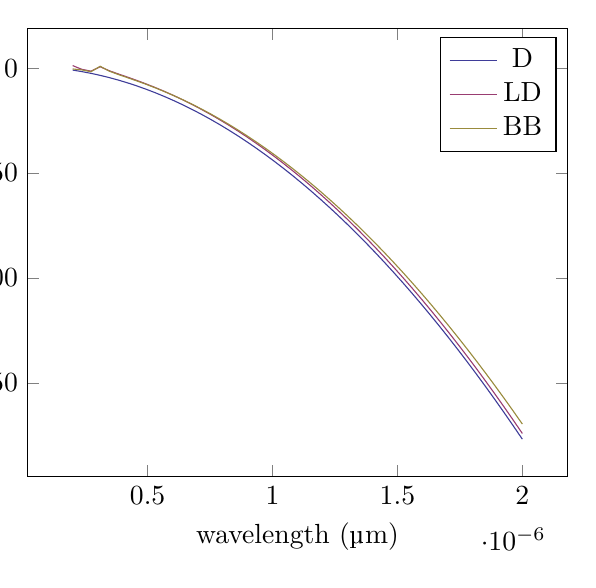
\begin{tikzpicture}[baseline,trim axis left]
			\begin{axis}[xlabel=wavelength (\si{\micro\meter}),ylabel=permittivity $\epsilon'$]
				\addplot[color=colora] coordinates {
						(2e-07, -0.7848740217446666)
						(2.3673469387755102e-07, -1.500696310342145)
						(2.7346938775510205e-07, -2.336893707274946)
						(3.1020408163265303e-07, -3.293445923443576)
						(3.4693877551020406e-07, -4.37032975161251)
						(3.836734693877551e-07, -5.567519067817526)
						(4.2040816326530607e-07, -6.8849848329496925)
						(4.571428571428571e-07, -8.32269509451583)
						(4.938775510204081e-07, -9.8806149885752)
						(5.306122448979591e-07, -11.558706741852301)
						(5.673469387755102e-07, -13.356929674025409)
						(6.040816326530612e-07, -15.275240200190702)
						(6.408163265306121e-07, -17.313591833501636)
						(6.775510204081632e-07, -19.47193518798332)
						(7.142857142857142e-07, -21.750217981521512)
						(7.510204081632653e-07, -24.148385039025932)
						(7.877551020408163e-07, -26.66637829576758)
						(8.244897959183672e-07, -29.304136800889573)
						(8.612244897959183e-07, -32.061596721091234)
						(8.979591836734693e-07, -34.93869134448486)
						(9.346938775510204e-07, -37.935351084624955)
						(9.714285714285713e-07, -41.05150348470918)
						(1.0081632653061223e-06, -44.28707322195098)
						(1.0448979591836734e-06, -47.64198211212275)
						(1.0816326530612245e-06, -51.11614911426981)
						(1.1183673469387754e-06, -54.70949033559387)
						(1.1551020408163265e-06, -58.42191903650631)
						(1.1918367346938776e-06, -62.25334563584963)
						(1.2285714285714284e-06, -66.20367771628757)
						(1.2653061224489795e-06, -70.27282002986261)
						(1.3020408163265306e-06, -74.46067450372047)
						(1.3387755102040815e-06, -78.76714024600066)
						(1.3755102040816325e-06, -83.19211355189331)
						(1.4122448979591836e-06, -87.7354879098602)
						(1.4489795918367345e-06, -92.39715400802062)
						(1.4857142857142856e-06, -97.17699974070077)
						(1.5224489795918367e-06, -102.07491021514564)
						(1.5591836734693875e-06, -107.0907677583933)
						(1.5959183673469386e-06, -112.2244519243105)
						(1.6326530612244897e-06, -117.47583950078872)
						(1.6693877551020408e-06, -122.84480451709986)
						(1.7061224489795917e-06, -128.3312182514113)
						(1.7428571428571427e-06, -133.93494923845853)
						(1.7795918367346938e-06, -139.65586327737546)
						(1.8163265306122447e-06, -145.49382343968065)
						(1.8530612244897958e-06, -151.44869007741977)
						(1.8897959183673469e-06, -157.52032083146185)
						(1.9265306122448977e-06, -163.70857063994956)
						(1.963265306122449e-06, -170.01329174690287)
						(2e-06, -176.43433371097328)
					};
				\addlegendentry{D}
				\addplot[color=colorb] coordinates {
						(2e-07, 1.359050982328245)
						(2.3673469387755102e-07, -0.42355364928957706)
						(2.7346938775510205e-07, -1.281143987206665)
						(3.1020408163265303e-07, 0.7882374791044482)
						(3.4693877551020406e-07, -1.1046110525286434)
						(3.836734693877551e-07, -2.647675306796513)
						(4.2040816326530607e-07, -4.153887245848895)
						(4.571428571428571e-07, -5.71060703393885)
						(4.938775510204081e-07, -7.34997666334408)
						(5.306122448979591e-07, -9.086621921820388)
						(5.673469387755102e-07, -10.928209257037828)
						(6.040816326530612e-07, -12.87917381057434)
						(6.408163265306121e-07, -14.942271468428904)
						(6.775510204081632e-07, -17.119307932279042)
						(7.142857142857142e-07, -19.411514295633282)
						(7.510204081632653e-07, -21.81975513257755)
						(7.877551020408163e-07, -24.344650785889158)
						(8.244897959183672e-07, -26.98665280867592)
						(8.612244897959183e-07, -29.746092434779854)
						(8.979591836734693e-07, -32.62321280900693)
						(9.346938775510204e-07, -35.618191056699644)
						(9.714285714285713e-07, -38.731153782608736)
						(1.0081632653061223e-06, -41.96218819670814)
						(1.0448979591836734e-06, -45.31135025543474)
						(1.0816326530612245e-06, -48.778670720383666)
						(1.1183673469387754e-06, -52.36415973511977)
						(1.1551020408163265e-06, -56.067810328987875)
						(1.1918367346938776e-06, -59.889601131789966)
						(1.2285714285714284e-06, -63.82949849992716)
						(1.2653061224489795e-06, -67.88745819803795)
						(1.3020408163265306e-06, -72.0634267410558)
						(1.3387755102040815e-06, -76.3573424741287)
						(1.3755102040816325e-06, -80.76913644825014)
						(1.4122448979591836e-06, -85.29873313528849)
						(1.4489795918367345e-06, -89.94605101574413)
						(1.4857142857142856e-06, -94.71100306489483)
						(1.5224489795918367e-06, -99.5934971572582)
						(1.5591836734693875e-06, -104.59343640497228)
						(1.5959183673469386e-06, -109.71071944239652)
						(1.6326530612244897e-06, -114.94524066670337)
						(1.6693877551020408e-06, -120.2968904422684)
						(1.7061224489795917e-06, -125.76555527513895)
						(1.7428571428571427e-06, -131.35111796265775)
						(1.7795918367346938e-06, -137.0534577223714)
						(1.8163265306122447e-06, -142.87245030359725)
						(1.8530612244897958e-06, -148.80796808441963)
						(1.8897959183673469e-06, -154.85988015640075)
						(1.9265306122448977e-06, -161.02805239889992)
						(1.963265306122449e-06, -167.31234754457728)
						(2e-06, -173.71262523739603)
					};
				\addlegendentry{LD}
				\addplot[color=colorc] coordinates {
						(2e-07, -0.24721746795050648)
						(2.3673469387755102e-07, -0.6914818429999761)
						(2.7346938775510205e-07, -1.5450619559511596)
						(3.1020408163265303e-07, 1.0336346694821135)
						(3.4693877551020406e-07, -1.31713668689564)
						(3.836734693877551e-07, -2.923708420943084)
						(4.2040816326530607e-07, -4.4267033331918615)
						(4.571428571428571e-07, -5.951889712102661)
						(4.938775510204081e-07, -7.545203403730973)
						(5.306122448979591e-07, -9.227710013998756)
						(5.673469387755102e-07, -11.010090574337369)
						(6.040816326530612e-07, -12.898215890134514)
						(6.408163265306121e-07, -14.895531768019898)
						(6.775510204081632e-07, -17.00416640958628)
						(7.142857142857142e-07, -19.225485365419015)
						(7.510204081632653e-07, -21.560389217670092)
						(7.877551020408163e-07, -24.009482744551715)
						(8.244897959183672e-07, -26.573175761323956)
						(8.612244897959183e-07, -29.251745654095693)
						(8.979591836734693e-07, -32.045377453396554)
						(9.346938775510204e-07, -34.954190235428904)
						(9.714285714285713e-07, -37.978254932663106)
						(1.0081632653061223e-06, -41.117606598818874)
						(1.0448979591836734e-06, -44.372253009336326)
						(1.0816326530612245e-06, -47.742180790374995)
						(1.1183673469387754e-06, -51.227359850548254)
						(1.1551020408163265e-06, -54.82774662807375)
						(1.1918367346938776e-06, -58.54328649900327)
						(1.2285714285714284e-06, -62.37391558339307)
						(1.2653061224489795e-06, -66.3195621141182)
						(1.3020408163265306e-06, -70.38014748440193)
						(1.3387755102040815e-06, -74.55558705687118)
						(1.3755102040816325e-06, -78.84579079389522)
						(1.4122448979591836e-06, -83.25066375278384)
						(1.4489795918367345e-06, -87.77010647793784)
						(1.4857142857142856e-06, -92.40401531380387)
						(1.5224489795918367e-06, -97.15228265651444)
						(1.5591836734693875e-06, -102.01479715772858)
						(1.5959183673469386e-06, -106.99144389096483)
						(1.6326530612244897e-06, -112.08210448832276)
						(1.6693877551020408e-06, -117.28665725369122)
						(1.7061224489795917e-06, -122.60497725718547)
						(1.7428571428571427e-06, -128.03693641452114)
						(1.7795918367346938e-06, -133.5824035542448)
						(1.8163265306122447e-06, -139.24124447512997)
						(1.8530612244897958e-06, -145.0133219955777)
						(1.8897959183673469e-06, -150.89849599648855)
						(1.9265306122448977e-06, -156.8966234587899)
						(1.963265306122449e-06, -163.00755849657028)
						(2e-06, -169.2311523865946)
					};
				\addlegendentry{BB}
			\end{axis}
		\end{tikzpicture}%
		\\
		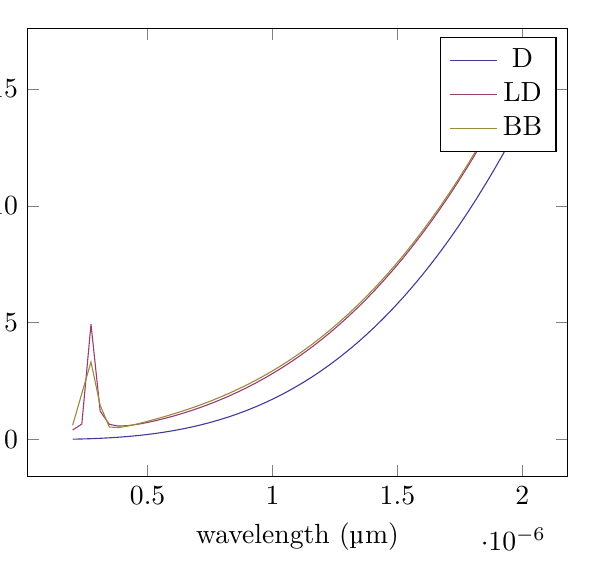
\begin{tikzpicture}[baseline,trim axis left]
			\begin{axis}[xlabel=wavelength (\si{\micro\meter}),ylabel=permittivity $\epsilon''$]
				\addplot[color=colora] coordinates {
						(2e-07, 0.013820140651214206)
						(2.3673469387755102e-07, 0.02291911064761145)
						(2.7346938775510205e-07, 0.035328564407303344)
						(3.1020408163265303e-07, 0.05156183964931969)
						(3.4693877551020406e-07, 0.0721321194793111)
						(3.836734693877551e-07, 0.09755241166003459)
						(4.2040816326530607e-07, 0.12833552789672326)
						(4.571428571428571e-07, 0.16499406313909548)
						(4.938775510204081e-07, 0.20804037490175553)
						(5.306122448979591e-07, 0.2579865626047377)
						(5.673469387755102e-07, 0.3153444469359391)
						(6.040816326530612e-07, 0.3806255492371874)
						(6.408163265306121e-07, 0.45434107091568154)
						(6.775510204081632e-07, 0.5370018728825463)
						(7.142857142857142e-07, 0.6291184550202302)
						(7.510204081632653e-07, 0.7312009356804758)
						(7.877551020408163e-07, 0.8437590312145905)
						(8.244897959183672e-07, 0.9673020355377348)
						(8.612244897959183e-07, 1.1023387997289422)
						(8.979591836734693e-07, 1.2493777116685787)
						(9.346938775510204e-07, 1.408926675714957)
						(9.714285714285713e-07, 1.5814930924217858)
						(1.0081632653061223e-06, 1.7675838382981686)
						(1.0448979591836734e-06, 1.9677052456128112)
						(1.0816326530612245e-06, 2.1823630822441547)
						(1.1183673469387754e-06, 2.4120625315780586)
						(1.1551020408163265e-06, 2.657308172454767)
						(1.1918367346938776e-06, 2.918603959166735)
						(1.2285714285714284e-06, 3.196453201509046)
						(1.2653061224489795e-06, 3.4913585448840165)
						(1.3020408163265306e-06, 3.8038219504616424)
						(1.3387755102040815e-06, 4.134344675397497)
						(1.3755102040816325e-06, 4.483427253109756)
						(1.4122448979591836e-06, 4.851569473616868)
						(1.4489795918367345e-06, 5.239270363937568)
						(1.4857142857142856e-06, 5.647028168554792)
						(1.5224489795918367e-06, 6.075340329945033)
						(1.5591836734693875e-06, 6.524703469174802)
						(1.5959183673469386e-06, 6.995613366565686)
						(1.6326530612244897e-06, 7.4885649424296075)
						(1.6693877551020408e-06, 8.004052237875781)
						(1.7061224489795917e-06, 8.542568395690992)
						(1.7428571428571427e-06, 9.1046056412946)
						(1.7795918367346938e-06, 9.690655263769909)
						(1.8163265306122447e-06, 10.301207596973283)
						(1.8530612244897958e-06, 10.93675200072266)
						(1.8897959183673469e-06, 11.59777684206675)
						(1.9265306122448977e-06, 12.284769476636546)
						(1.963265306122449e-06, 12.998216230080592)
						(2e-06, 13.738602379585318)
					};
				\addlegendentry{D}
				\addplot[color=colorb] coordinates {
						(2e-07, 0.4048352105427265)
						(2.3673469387755102e-07, 0.6641336946861055)
						(2.7346938775510205e-07, 4.934632098078845)
						(3.1020408163265303e-07, 1.212783069063026)
						(3.4693877551020406e-07, 0.6490640670957781)
						(3.836734693877551e-07, 0.5750569237442578)
						(4.2040816326530607e-07, 0.5932442217518595)
						(4.571428571428571e-07, 0.6457958076564755)
						(4.938775510204081e-07, 0.7172949477371516)
						(5.306122448979591e-07, 0.8022264754618131)
						(5.673469387755102e-07, 0.8983147685547268)
						(6.040816326530612e-07, 1.0045982261350381)
						(6.408163265306121e-07, 1.120734083220734)
						(6.775510204081632e-07, 1.2467043967645695)
						(7.142857142857142e-07, 1.3826760234490958)
						(7.510204081632653e-07, 1.52892752802846)
						(7.877551020408163e-07, 1.6858081802242904)
						(8.244897959183672e-07, 1.8537136015500706)
						(8.612244897959183e-07, 2.033070626473662)
						(8.979591836734693e-07, 2.2243275397490847)
						(9.346938775510204e-07, 2.427947590105134)
						(9.714285714285713e-07, 2.644404573841871)
						(1.0081632653061223e-06, 2.874179765885631)
						(1.0448979591836734e-06, 3.117759750256305)
						(1.0816326530612245e-06, 3.3756348636852804)
						(1.1183673469387754e-06, 3.6482980647869283)
						(1.1551020408163265e-06, 3.9362441031411093)
						(1.1918367346938776e-06, 4.23996890254476)
						(1.2285714285714284e-06, 4.55996909896015)
						(1.2653061224489795e-06, 4.896741691318022)
						(1.3020408163265306e-06, 5.25078377536813)
						(1.3387755102040815e-06, 5.622592339107126)
						(1.3755102040816325e-06, 6.012664104166902)
						(1.4122448979591836e-06, 6.4214954017040204)
						(1.4489795918367345e-06, 6.8495820743159)
						(1.4857142857142856e-06, 7.297419397672424)
						(1.5224489795918367e-06, 7.765502017133128)
						(1.5591836734693875e-06, 8.2543238957853)
						(1.5959183673469386e-06, 8.76437827120281)
						(1.6326530612244897e-06, 9.296157618871376)
						(1.6693877551020408e-06, 9.85015362071103)
						(1.7061224489795917e-06, 10.426857137493363)
						(1.7428571428571427e-06, 11.02675818422916)
						(1.7795918367346938e-06, 11.650345907814637)
						(1.8163265306122447e-06, 12.298108566386865)
						(1.8530612244897958e-06, 12.970533509964264)
						(1.8897959183673469e-06, 13.668107162044162)
						(1.9265306122448977e-06, 14.391315001904445)
						(1.963265306122449e-06, 15.140641547414042)
						(2e-06, 15.916570338202005)
					};
				\addlegendentry{LD}
				\addplot[color=colorc] coordinates {
						(2e-07, 0.6102901232609813)
						(2.3673469387755102e-07, 1.9701145952419097)
						(2.7346938775510205e-07, 3.317004579724485)
						(3.1020408163265303e-07, 1.4595320972902277)
						(3.4693877551020406e-07, 0.5353229068723269)
						(3.836734693877551e-07, 0.5115280150626041)
						(4.2040816326530607e-07, 0.5743575874075902)
						(4.571428571428571e-07, 0.6633639854437718)
						(4.938775510204081e-07, 0.7625109516321108)
						(5.306122448979591e-07, 0.8679150462185126)
						(5.673469387755102e-07, 0.9790656583302688)
						(6.040816326530612e-07, 1.0963972807342148)
						(6.408163265306121e-07, 1.2205966853369872)
						(6.775510204081632e-07, 1.3523967239212713)
						(7.142857142857142e-07, 1.492514885073333)
						(7.510204081632653e-07, 1.6416375204404225)
						(7.877551020408163e-07, 1.8004188808309958)
						(8.244897959183672e-07, 1.9694846912210204)
						(8.612244897959183e-07, 2.149436702594483)
						(8.979591836734693e-07, 2.340856999961308)
						(9.346938775510204e-07, 2.5443117027881543)
						(9.714285714285713e-07, 2.7603540109977462)
						(1.0081632653061223e-06, 2.989526660216237)
						(1.0448979591836734e-06, 3.2323638798162078)
						(1.0816326530612245e-06, 3.489392946314058)
						(1.1183673469387754e-06, 3.761135413114617)
						(1.1551020408163265e-06, 4.0481080836967465)
						(1.1918367346938776e-06, 4.350823782283239)
						(1.2285714285714284e-06, 4.669791964874221)
						(1.2653061224489795e-06, 5.0055192043921375)
						(1.3020408163265306e-06, 5.358509576396205)
						(1.3387755102040815e-06, 5.7292649660815265)
						(1.3755102040816325e-06, 6.118285312787323)
						(1.4122448979591836e-06, 6.526068804739895)
						(1.4489795918367345e-06, 6.953112034033628)
						(1.4857142857142856e-06, 7.3999101197344235)
						(1.5224489795918367e-06, 7.866956805338521)
						(1.5591836734693875e-06, 8.35474453553042)
						(1.5959183673469386e-06, 8.863764516173827)
						(1.6326530612244897e-06, 9.394506760677157)
						(1.6693877551020408e-06, 9.947460125250796)
						(1.7061224489795917e-06, 10.523112335080363)
						(1.7428571428571427e-06, 11.121950003049054)
						(1.7795918367346938e-06, 11.744458642331512)
						(1.8163265306122447e-06, 12.3911226739333)
						(1.8530612244897958e-06, 13.06242543005178)
						(1.8897959183673469e-06, 13.758849153974042)
						(1.9265306122448977e-06, 14.480874997099562)
						(1.963265306122449e-06, 15.228983013570835)
						(2e-06, 16.003652152910867)
					};
				\addlegendentry{BB}
			\end{axis}
		\end{tikzpicture}%
		\\
		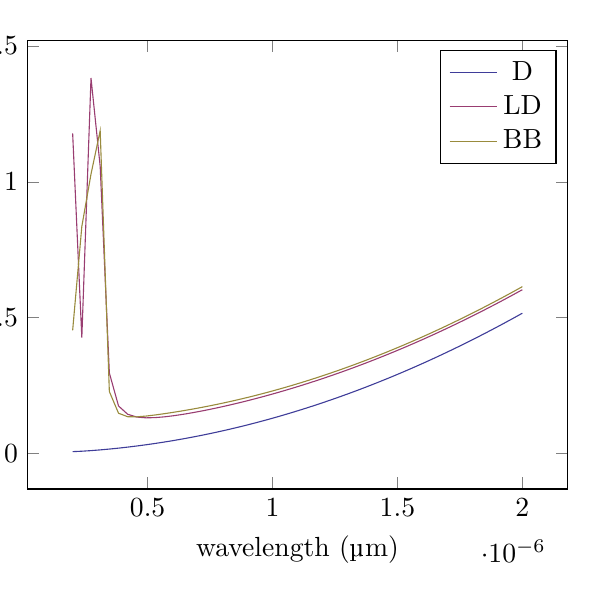
\begin{tikzpicture}[baseline,trim axis left]
			\begin{axis}[xlabel=wavelength (\si{\micro\meter}),ylabel=refractive index $n'$]
				\addplot[color=colora] coordinates {
						(2e-07, 0.0077994802114394555)
						(2.3673469387755102e-07, 0.009354244069745549)
						(2.7346938775510205e-07, 0.011554844593555885)
						(3.1020408163265303e-07, 0.01420560828378247)
						(3.4693877551020406e-07, 0.01725149781042338)
						(3.836734693877551e-07, 0.020670952712057537)
						(4.2040816326530607e-07, 0.024453811066897316)
						(4.571428571428571e-07, 0.02859466397532551)
						(4.938775510204081e-07, 0.03309036675830158)
						(5.306122448979591e-07, 0.03793896062896816)
						(5.673469387755102e-07, 0.04313915359836002)
						(6.040816326530612e-07, 0.04869004974191256)
						(6.408163265306121e-07, 0.054590998777817895)
						(6.775510204081632e-07, 0.060841508088546874)
						(7.142857142857142e-07, 0.06744118902543195)
						(7.510204081632653e-07, 0.07438972293768238)
						(7.877551020408163e-07, 0.08168683900842261)
						(8.244897959183672e-07, 0.08933229940319612)
						(8.612244897959183e-07, 0.09732588908341566)
						(8.979591836734693e-07, 0.10566740867365086)
						(9.346938775510204e-07, 0.1143566693751254)
						(9.714285714285713e-07, 0.1233934892781885)
						(1.0081632653061223e-06, 0.13277769064948905)
						(1.0448979591836734e-06, 0.14250909790920815)
						(1.0816326530612245e-06, 0.15258753610471756)
						(1.1183673469387754e-06, 0.16301282974612302)
						(1.1551020408163265e-06, 0.1737848019088628)
						(1.1918367346938776e-06, 0.18490327353607738)
						(1.2285714285714284e-06, 0.1963680628916576)
						(1.2653061224489795e-06, 0.2081789851284019)
						(1.3020408163265306e-06, 0.22033585194454175)
						(1.3387755102040815e-06, 0.23283847130926064)
						(1.3755102040816325e-06, 0.2456866472421145)
						(1.4122448979591836e-06, 0.25888017963473087)
						(1.4489795918367345e-06, 0.27241886410672744)
						(1.4857142857142856e-06, 0.2863024918883639)
						(1.5224489795918367e-06, 0.3005308497251957)
						(1.5591836734693875e-06, 0.3151037198005309)
						(1.5959183673469386e-06, 0.33002087967209787)
						(1.6326530612244897e-06, 0.3452821022207534)
						(1.6693877551020408e-06, 0.3608871556090487)
						(1.7061224489795917e-06, 0.37683580324766563)
						(1.7428571428571427e-06, 0.3931278037689519)
						(1.7795918367346938e-06, 0.40976291100596496)
						(1.8163265306122447e-06, 0.4267408739762741)
						(1.8530612244897958e-06, 0.4440614368700694)
						(1.8897959183673469e-06, 0.46172433904150867)
						(1.9265306122448977e-06, 0.4797293150031158)
						(1.963265306122449e-06, 0.49807609442275286)
						(2e-06, 0.5167644021228207)
					};
				\addlegendentry{D}
				\addplot[color=colorb] coordinates {
						(2e-07, 1.1783711132618022)
						(2.3673469387755102e-07, 0.4267003225643034)
						(2.7346938775510205e-07, 1.3814998252140789)
						(3.1020408163265303e-07, 1.0570401946414625)
						(3.4693877551020406e-07, 0.29713607868819564)
						(3.836734693877551e-07, 0.1756838191685956)
						(4.2040816326530607e-07, 0.1451701340329712)
						(4.571428571428571e-07, 0.1349065812926932)
						(4.938775510204081e-07, 0.13213248427563817)
						(5.306122448979591e-07, 0.13293638299108437)
						(5.673469387755102e-07, 0.13575572345069098)
						(6.040816326530612e-07, 0.13985849945992782)
						(6.408163265306121e-07, 0.14486368120723764)
						(6.775510204081632e-07, 0.1505577305100302)
						(7.142857142857142e-07, 0.15681435553626238)
						(7.510204081632653e-07, 0.16355578655906217)
						(7.877551020408163e-07, 0.17073263218512186)
						(8.244897959183672e-07, 0.17831276712276337)
						(8.612244897959183e-07, 0.18627490791197487)
						(8.979591836734693e-07, 0.19460475478299935)
						(9.346938775510204e-07, 0.20329260084273568)
						(9.714285714285713e-07, 0.21233181132673626)
						(1.0081632653061223e-06, 0.22171783478642199)
						(1.0448979591836734e-06, 0.23144754805703618)
						(1.0816326530612245e-06, 0.24151881539402542)
						(1.1183673469387754e-06, 0.25193018770648107)
						(1.1551020408163265e-06, 0.26268069498529734)
						(1.1918367346938776e-06, 0.2737697016427112)
						(1.2285714285714284e-06, 0.28519680486991983)
						(1.2653061224489795e-06, 0.2969617627447383)
						(1.3020408163265306e-06, 0.30906444311833714)
						(1.3387755102040815e-06, 0.3215047871416539)
						(1.3755102040816325e-06, 0.3342827831840542)
						(1.4122448979591836e-06, 0.3473984481767801)
						(1.4489795918367345e-06, 0.36085181428970464)
						(1.4857142857142856e-06, 0.3746429194562909)
						(1.5224489795918367e-06, 0.38877180068389705)
						(1.5591836734693875e-06, 0.40323848938518864)
						(1.5959183673469386e-06, 0.41804300817716267)
						(1.6326530612244897e-06, 0.433185368745762)
						(1.6693877551020408e-06, 0.448665570482642)
						(1.7061224489795917e-06, 0.4644835996791444)
						(1.7428571428571427e-06, 0.48063942912005225)
						(1.7795918367346938e-06, 0.4971330179612433)
						(1.8163265306122447e-06, 0.5139643118060373)
						(1.8530612244897958e-06, 0.5311332429179383)
						(1.8897959183673469e-06, 0.5486397305238192)
						(1.9265306122448977e-06, 0.5664836811739009)
						(1.963265306122449e-06, 0.5846649891346085)
						(2e-06, 0.6031835367963474)
					};
				\addlegendentry{LD}
				\addplot[color=colorc] coordinates {
						(2e-07, 0.45345520472678824)
						(2.3673469387755102e-07, 0.8356014018642134)
						(2.7346938775510205e-07, 1.0281383273141127)
						(3.1020408163265303e-07, 1.1878778056487425)
						(3.4693877551020406e-07, 0.22872440042735057)
						(3.836734693877551e-07, 0.14901480143606538)
						(4.2040816326530607e-07, 0.13620842625815055)
						(4.571428571428571e-07, 0.13574480611862905)
						(4.938775510204081e-07, 0.13862076719748326)
						(5.306122448979591e-07, 0.14269921867384255)
						(5.673469387755102e-07, 0.14738672469106795)
						(6.040816326530612e-07, 0.15250424569472135)
						(6.408163265306121e-07, 0.15799763075810228)
						(6.775510204081632e-07, 0.16385279709061343)
						(7.142857142857142e-07, 0.17006838332623225)
						(7.510204081632653e-07, 0.1766464562650421)
						(7.877551020408163e-07, 0.18358937301672035)
						(8.244897959183672e-07, 0.19089884144062455)
						(8.612244897959183e-07, 0.19857576567587595)
						(8.979591836734693e-07, 0.20662035055881225)
						(9.346938775510204e-07, 0.21503226791707408)
						(9.714285714285713e-07, 0.22381081463298666)
						(1.0081632653061223e-06, 0.23295504175622783)
						(1.0448979591836734e-06, 0.2424638525751642)
						(1.0816326530612245e-06, 0.25233607383168893)
						(1.1183673469387754e-06, 0.2625705056664088)
						(1.1551020408163265e-06, 0.273165955493376)
						(1.1918367346938776e-06, 0.28412126008520894)
						(1.2285714285714284e-06, 0.29543529919225536)
						(1.2653061224489795e-06, 0.3071070031918654)
						(1.3020408163265306e-06, 0.31913535660329234)
						(1.3387755102040815e-06, 0.3315193987986799)
						(1.3755102040816325e-06, 0.34425822286274427)
						(1.4122448979591836e-06, 0.3573509732771731)
						(1.4489795918367345e-06, 0.3707968429035332)
						(1.4857142857142856e-06, 0.38459506959361356)
						(1.5224489795918367e-06, 0.39874493265120675)
						(1.5591836734693875e-06, 0.41324574929570534)
						(1.5959183673469386e-06, 0.4280968712250534)
						(1.6326530612244897e-06, 0.44329768133838204)
						(1.6693877551020408e-06, 0.4588475906533129)
						(1.7061224489795917e-06, 0.4747460354350706)
						(1.7428571428571427e-06, 0.49099247454234335)
						(1.7795918367346938e-06, 0.5075863869871761)
						(1.8163265306122447e-06, 0.5245272697009496)
						(1.8530612244897958e-06, 0.5418146354954317)
						(1.8897959183673469e-06, 0.5594480112062957)
						(1.9265306122448977e-06, 0.5774269360056727)
						(1.963265306122449e-06, 0.5957509598703211)
						(2e-06, 0.6144196421922116)
					};
				\addlegendentry{BB}
			\end{axis}
		\end{tikzpicture}%
		\\
		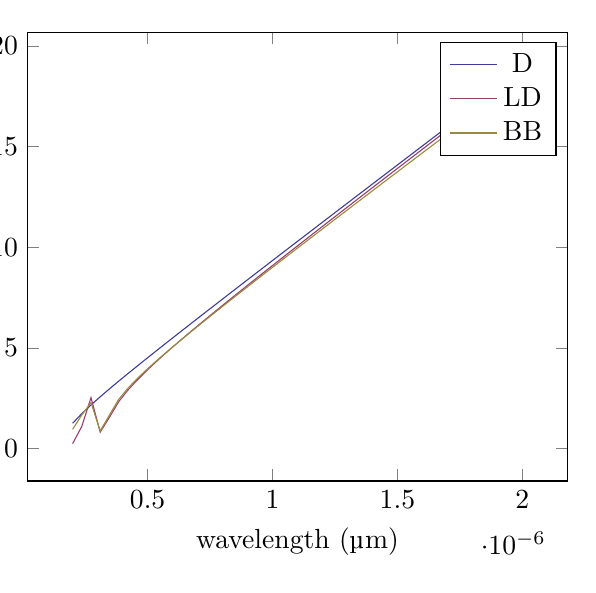
\begin{tikzpicture}[baseline,trim axis left]
			\begin{axis}[xlabel=wavelength (\si{\micro\meter}),ylabel=refractive index $n''$]
				\addplot[color=colora] coordinates {
						(2e-07, 1.2529444150769302)
						(2.3673469387755102e-07, 1.7325032826660165)
						(2.7346938775510205e-07, 2.1619561613078684)
						(3.1020408163265303e-07, 2.566572704113518)
						(3.4693877551020406e-07, 2.9565613018468646)
						(3.836734693877551e-07, 3.3370485031247448)
						(4.2040816326530607e-07, 3.7109521209051963)
						(4.571428571428571e-07, 4.080076653525934)
						(4.938775510204081e-07, 4.445606811436972)
						(5.306122448979591e-07, 4.808356498136532)
						(5.673469387755102e-07, 5.168905234302248)
						(6.040816326530612e-07, 5.527677798340741)
						(6.408163265306121e-07, 5.884993119902384)
						(6.775510204081632e-07, 6.241095557206252)
						(7.142857142857142e-07, 6.596175603408186)
						(7.510204081632653e-07, 6.950383999449913)
						(7.877551020408163e-07, 7.3038415967810755)
						(8.244897959183672e-07, 7.656646401735714)
						(8.612244897959183e-07, 8.008878704260304)
						(8.979591836734693e-07, 8.360604875933399)
						(9.346938775510204e-07, 8.711880225583398)
						(9.714285714285713e-07, 9.062751175874292)
						(1.0081632653061223e-06, 9.413256942959244)
						(1.0448979591836734e-06, 9.763430847310758)
						(1.0816326530612245e-06, 10.113301347279663)
						(1.1183673469387754e-06, 10.462892861752499)
						(1.1551020408163265e-06, 10.812226430655327)
						(1.1918367346938776e-06, 11.161320249541626)
						(1.2285714285714284e-06, 11.510190105503156)
						(1.2653061224489795e-06, 11.858849735089125)
						(1.3020408163265306e-06, 12.207311120092957)
						(1.3387755102040815e-06, 12.55558473347397)
						(1.3755102040816325e-06, 12.903679744981769)
						(1.4122448979591836e-06, 13.251604194003676)
						(1.4489795918367345e-06, 13.59936513558937)
						(1.4857142857142856e-06, 13.946968764399113)
						(1.5224489795918367e-06, 14.294420520383621)
						(1.5591836734693875e-06, 14.641725179269375)
						(1.5959183673469386e-06, 14.988886930344764)
						(1.6326530612244897e-06, 15.335909443583885)
						(1.6693877551020408e-06, 15.68279592777917)
						(1.7061224489795917e-06, 16.02954918106062)
						(1.7428571428571427e-06, 16.37617163494293)
						(1.7795918367346938e-06, 16.72266539285)
						(1.8163265306122447e-06, 17.06903226391014)
						(1.8530612244897958e-06, 17.41527379268755)
						(1.8897959183673469e-06, 17.761391285410337)
						(1.9265306122448977e-06, 18.1073858331689)
						(1.963265306122449e-06, 18.453258332486342)
						(2e-06, 18.79900950360282)
					};
				\addlegendentry{D}
				\addplot[color=colorb] coordinates {
						(2e-07, 0.24293002384066908)
						(2.3673469387755102e-07, 1.1005696839056196)
						(2.7346938775510205e-07, 2.525741773924324)
						(3.1020408163265303e-07, 0.8112909391620408)
						(3.4693877551020406e-07, 1.5446040928256284)
						(3.836734693877551e-07, 2.3145367187038435)
						(4.2040816326530607e-07, 2.889623371190109)
						(4.571428571428571e-07, 3.384909694398045)
						(4.938775510204081e-07, 3.8386027814153763)
						(5.306122448979591e-07, 4.267152212833084)
						(5.673469387755102e-07, 4.6790252988175745)
						(6.040816326530612e-07, 5.0791208314915135)
						(6.408163265306121e-07, 5.4705131303309775)
						(6.775510204081632e-07, 5.855249877246124)
						(7.142857142857142e-07, 6.2347582210917425)
						(7.510204081632653e-07, 6.610068929730537)
						(7.877551020408163e-07, 6.981948212008167)
						(8.244897959183672e-07, 7.350979288719959)
						(8.612244897959183e-07, 7.717615017101782)
						(8.979591836734693e-07, 8.082213040942571)
						(9.346938775510204e-07, 8.445059968793242)
						(9.714285714285713e-07, 8.806388428942938)
						(1.0081632653061223e-06, 9.16638936495396)
						(1.0448979591836734e-06, 9.525221070708685)
						(1.0816326530612245e-06, 9.883015942370324)
						(1.1183673469387754e-06, 10.239885600395894)
						(1.1551020408163265e-06, 10.595924827640657)
						(1.1918367346938776e-06, 10.951214634124153)
						(1.2285714285714284e-06, 11.30582466850032)
						(1.2653061224489795e-06, 11.659815134604015)
						(1.3020408163265306e-06, 12.01323832869854)
						(1.3387755102040815e-06, 12.366139882945179)
						(1.3755102040816325e-06, 12.718559779108908)
						(1.4122448979591836e-06, 13.07053318094439)
						(1.4489795918367345e-06, 13.422091122296875)
						(1.4857142857142856e-06, 13.77326107949701)
						(1.5224489795918367e-06, 14.124067450296689)
						(1.5591836734693875e-06, 14.474531956805645)
						(1.5959183673469386e-06, 14.824673986235402)
						(1.6326530612244897e-06, 15.174510880446775)
						(1.6693877551020408e-06, 15.524058183117257)
						(1.7061224489795917e-06, 15.873329851641707)
						(1.7428571428571427e-06, 16.222338439539634)
						(1.7795918367346938e-06, 16.571095254081346)
						(1.8163265306122447e-06, 16.919610492999386)
						(1.8530612244897958e-06, 17.267893363473853)
						(1.8897959183673469e-06, 17.615952186033542)
						(1.9265306122448977e-06, 17.963794485572155)
						(1.963265306122449e-06, 18.3114270713179)
						(2e-06, 18.65885610729973)
					};
				\addlegendentry{LD}
				\addplot[color=colorc] coordinates {
						(2e-07, 0.9516712569415133)
						(2.3673469387755102e-07, 1.6671601877428666)
						(2.7346938775510205e-07, 2.2812848906015315)
						(3.1020408163265303e-07, 0.8688141477563064)
						(3.4693877551020406e-07, 1.6549631646936986)
						(3.836734693877551e-07, 2.4273087286087502)
						(4.2040816326530607e-07, 2.9816961845820518)
						(4.571428571428571e-07, 3.4555220631594423)
						(4.938775510204081e-07, 3.8895807282609245)
						(5.306122448979591e-07, 4.300714610622026)
						(5.673469387755102e-07, 4.69719350696829)
						(6.040816326530612e-07, 5.083595860233075)
						(6.408163265306121e-07, 5.462690732477004)
						(6.775510204081632e-07, 5.836268353785782)
						(7.142857142857142e-07, 6.205547295835592)
						(7.510204081632653e-07, 6.571391509898203)
						(7.877551020408163e-07, 6.9344340507984334)
						(8.244897959183672e-07, 7.295151558259407)
						(8.612244897959183e-07, 7.653911155586986)
						(8.979591836734693e-07, 8.011001113801147)
						(9.346938775510204e-07, 8.366651553838544)
						(9.714285714285713e-07, 8.721048814610521)
						(1.0081632653061223e-06, 9.07434566790339)
						(1.0448979591836734e-06, 9.426668736000211)
						(1.0816326530612245e-06, 9.77812398004155)
						(1.1183673469387754e-06, 10.128800829416498)
						(1.1551020408163265e-06, 10.478775335631006)
						(1.1918367346938776e-06, 10.828112613880194)
						(1.2285714285714284e-06, 11.17686875644533)
						(1.2653061224489795e-06, 11.525092348916576)
						(1.3020408163265306e-06, 11.872825683908296)
						(1.3387755102040815e-06, 12.220105741657967)
						(1.3755102040816325e-06, 12.56696498904201)
						(1.4122448979591836e-06, 12.91343203574371)
						(1.4489795918367345e-06, 13.259532177014774)
						(1.4857142857142856e-06, 13.605287845639987)
						(1.5224489795918367e-06, 13.950718990634817)
						(1.5591836734693875e-06, 14.295843396389005)
						(1.5959183673469386e-06, 14.640676953072731)
						(1.6326530612244897e-06, 14.98523388690365)
						(1.6693877551020408e-06, 15.329526957159478)
						(1.7061224489795917e-06, 15.673567625486342)
						(1.7428571428571427e-06, 16.017366202005768)
						(1.7795918367346938e-06, 16.360931971895702)
						(1.8163265306122447e-06, 16.704273305462284)
						(1.8530612244897958e-06, 17.047397754191973)
						(1.8897959183673469e-06, 17.3903121348486)
						(1.9265306122448977e-06, 17.733022603336117)
						(1.963265306122449e-06, 18.075534719767305)
						(2e-06, 18.417853505949395)
					};
				\addlegendentry{BB}
			\end{axis}
		\end{tikzpicture}%
		\\
	\end{tabular}
	\caption{Complex permittivity $\epsilon = \epsilon' + \mi \epsilon''$ and refractive index $n = n' + \mi n''$ for Ag based on the Drude (D), Lorentz-Drude (LD), and Brendel-Bormann (BB) models.}
\end{figure}
\clearpage
\newpage
\subsection{Al}
\begin{figure}[h!]
	\centering
	\begin{tabular}{l}
		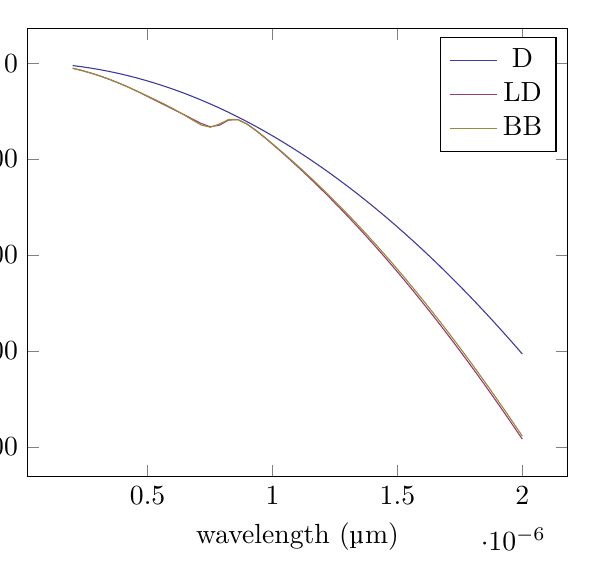
\begin{tikzpicture}[baseline,trim axis left]
			\begin{axis}[xlabel=wavelength (\si{\micro\meter}),ylabel=permittivity $\epsilon'$]
				\addplot[color=colora] coordinates {
						(2e-07, -2.0537091246449597)
						(2.3673469387755102e-07, -3.2784009504972405)
						(2.7346938775510205e-07, -4.7090441901649065)
						(3.1020408163265303e-07, -6.345605562070231)
						(3.4693877551020406e-07, -8.18804699758391)
						(3.836734693877551e-07, -10.236325643238496)
						(4.2040816326530607e-07, -12.490393863219678)
						(4.571428571428571e-07, -14.95019924213518)
						(4.938775510204081e-07, -17.61568458806089)
						(5.306122448979591e-07, -20.486787935863983)
						(5.673469387755102e-07, -23.563442550802627)
						(6.040816326530612e-07, -26.84557693240187)
						(6.408163265306121e-07, -30.333114818605306)
						(6.775510204081632e-07, -34.025975190202146)
						(7.142857142857142e-07, -37.92407227552903)
						(7.510204081632653e-07, -42.02731555544624)
						(7.877551020408163e-07, -46.33560976858776)
						(8.244897959183672e-07, -50.84885491688447)
						(8.612244897959183e-07, -55.56694627136013)
						(8.979591836734693e-07, -60.48977437819912)
						(9.346938775510204e-07, -65.6172250650859)
						(9.714285714285713e-07, -70.94917944781477)
						(1.0081632653061223e-06, -76.48551393716996)
						(1.0448979591836734e-06, -82.22610024607448)
						(1.0816326530612245e-06, -88.17080539700804)
						(1.1183673469387754e-06, -94.31949172969182)
						(1.1551020408163265e-06, -100.67201690904103)
						(1.1918367346938776e-06, -107.22823393338244)
						(1.2285714285714284e-06, -113.98799114293766)
						(1.2653061224489795e-06, -120.95113222857047)
						(1.3020408163265306e-06, -128.11749624079718)
						(1.3387755102040815e-06, -135.48691759905938)
						(1.3755102040816325e-06, -143.05922610125813)
						(1.4122448979591836e-06, -150.83424693354797)
						(1.4489795918367345e-06, -158.81180068039052)
						(1.4857142857142856e-06, -166.99170333486617)
						(1.5224489795918367e-06, -175.3737663092426)
						(1.5591836734693875e-06, -183.95779644579923)
						(1.5959183673469386e-06, -192.7435960279066)
						(1.6326530612244897e-06, -201.7309627913591)
						(1.6693877551020408e-06, -210.91968993596006)
						(1.7061224489795917e-06, -220.30956613735833)
						(1.7428571428571427e-06, -229.90037555913406)
						(1.7795918367346938e-06, -239.6918978651338)
						(1.8163265306122447e-06, -249.6839082320519)
						(1.8530612244897958e-06, -259.8761773622592)
						(1.8897959183673469e-06, -270.26847149687507)
						(1.9265306122448977e-06, -280.8605524290828)
						(1.963265306122449e-06, -291.6521775176882)
						(2e-06, -302.64309970091597)
					};
				\addlegendentry{D}
				\addplot[color=colorb] coordinates {
						(2e-07, -4.845612989503891)
						(2.3673469387755102e-07, -7.184061845921279)
						(2.7346938775510205e-07, -9.891461482901509)
						(3.1020408163265303e-07, -12.95236834932403)
						(3.4693877551020406e-07, -16.366606859582237)
						(3.836734693877551e-07, -20.145716783588284)
						(4.2040816326530607e-07, -24.285910259855086)
						(4.571428571428571e-07, -28.74414554747856)
						(4.938775510204081e-07, -33.43334029637763)
						(5.306122448979591e-07, -38.235153384078146)
						(5.673469387755102e-07, -43.03454620471178)
						(6.040816326530612e-07, -47.77939884193562)
						(6.408163265306121e-07, -52.53583350100591)
						(6.775510204081632e-07, -57.44519311054875)
						(7.142857142857142e-07, -62.37081504987511)
						(7.510204081632653e-07, -65.80706832114622)
						(7.877551020408163e-07, -64.13091317895577)
						(8.244897959183672e-07, -58.86050004933716)
						(8.612244897959183e-07, -58.377059943530114)
						(8.979591836734693e-07, -63.04105069972317)
						(9.346938775510204e-07, -69.93813633943626)
						(9.714285714285713e-07, -77.67791684144048)
						(1.0081632653061223e-06, -85.8129193507109)
						(1.0448979591836734e-06, -94.21200117169201)
						(1.0816326530612245e-06, -102.83964313547597)
						(1.1183673469387754e-06, -111.6886528646755)
						(1.1551020408163265e-06, -120.75975366802358)
						(1.1918367346938776e-06, -130.05535259153635)
						(1.2285714285714284e-06, -139.57770230353188)
						(1.2653061224489795e-06, -149.32844344262594)
						(1.3020408163265306e-06, -159.30856994614072)
						(1.3387755102040815e-06, -169.5185087842645)
						(1.3755102040816325e-06, -179.95821675379784)
						(1.4122448979591836e-06, -190.62726659949018)
						(1.4489795918367345e-06, -201.5249172229341)
						(1.4857142857142856e-06, -212.65016939276313)
						(1.5224489795918367e-06, -224.00180980183416)
						(1.5591836734693875e-06, -235.57844615784214)
						(1.5959183673469386e-06, -247.37853546161986)
						(1.6326530612244897e-06, -259.4004071025933)
						(1.6693877551020408e-06, -271.6422819783481)
						(1.7061224489795917e-06, -284.10228852885217)
						(1.7428571428571427e-06, -296.7784763455834)
						(1.7795918367346938e-06, -309.66882784965736)
						(1.8163265306122447e-06, -322.77126841297684)
						(1.8530612244897958e-06, -336.08367520903334)
						(1.8897959183673469e-06, -349.60388501571214)
						(1.9265306122448977e-06, -363.32970114462285)
						(1.963265306122449e-06, -377.2588996354249)
						(2e-06, -391.389234826111)
					};
				\addlegendentry{LD}
				\addplot[color=colorc] coordinates {
						(2e-07, -4.832847027277685)
						(2.3673469387755102e-07, -7.139090182726671)
						(2.7346938775510205e-07, -9.834067422586358)
						(3.1020408163265303e-07, -12.921462777468813)
						(3.4693877551020406e-07, -16.387681882556357)
						(3.836734693877551e-07, -20.19825368351809)
						(4.2040816326530607e-07, -24.29423114859795)
						(4.571428571428571e-07, -28.59716970188754)
						(4.938775510204081e-07, -33.03322572388798)
						(5.306122448979591e-07, -37.57290730057064)
						(5.673469387755102e-07, -42.263524154139695)
						(6.040816326530612e-07, -47.23032324799995)
						(6.408163265306121e-07, -52.62693575384632)
						(6.775510204081632e-07, -58.45622500528772)
						(7.142857142857142e-07, -63.94144018544523)
						(7.510204081632653e-07, -66.30160951690948)
						(7.877551020408163e-07, -62.89841535603955)
						(8.244897959183672e-07, -58.21172300096274)
						(8.612244897959183e-07, -58.308700231264915)
						(8.979591836734693e-07, -62.935401356751385)
						(9.346938775510204e-07, -69.7204598067243)
						(9.714285714285713e-07, -77.33998952679585)
						(1.0081632653061223e-06, -85.32713740888322)
						(1.0448979591836734e-06, -93.55001926604957)
						(1.0816326530612245e-06, -101.98211134528246)
						(1.1183673469387754e-06, -110.62604305531596)
						(1.1551020408163265e-06, -119.49038999906828)
						(1.1918367346938776e-06, -128.58313672232833)
						(1.2285714285714284e-06, -137.91023876379623)
						(1.2653061224489795e-06, -147.4756610686732)
						(1.3020408163265306e-06, -157.2817635589276)
						(1.3387755102040815e-06, -167.32969702719942)
						(1.3755102040816325e-06, -177.61972524121228)
						(1.4122448979591836e-06, -188.15146677096004)
						(1.4489795918367345e-06, -198.9240705123401)
						(1.4857142857142856e-06, -209.93634129291874)
						(1.5224489795918367e-06, -221.1868293648069)
						(1.5591836734693875e-06, -232.67389424524922)
						(1.5959183673469386e-06, -244.39575047852864)
						(1.6326530612244897e-06, -256.3505006868621)
						(1.6693877551020408e-06, -268.53615967767183)
						(1.7061224489795917e-06, -280.95067224188745)
						(1.7428571428571427e-06, -293.5919264854347)
						(1.7795918367346938e-06, -306.4577639842735)
						(1.8163265306122447e-06, -319.545987669492)
						(1.8530612244897958e-06, -332.85436808159824)
						(1.8897959183673469e-06, -346.3806484464048)
						(1.9265306122448977e-06, -360.12254889402755)
						(1.963265306122449e-06, -374.0777700504278)
						(2e-06, -388.24399616585475)
					};
				\addlegendentry{BB}
			\end{axis}
		\end{tikzpicture}%
		\\
		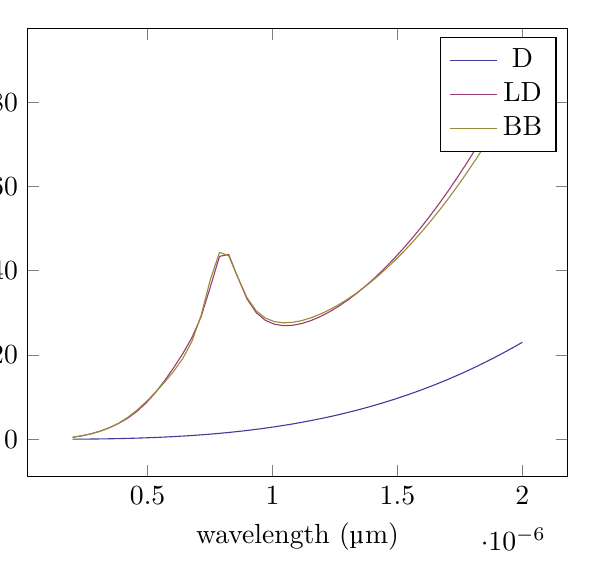
\begin{tikzpicture}[baseline,trim axis left]
			\begin{axis}[xlabel=wavelength (\si{\micro\meter}),ylabel=permittivity $\epsilon''$]
				\addplot[color=colora] coordinates {
						(2e-07, 0.023152035609705638)
						(2.3673469387755102e-07, 0.03839502109844504)
						(2.7346938775510205e-07, 0.05918390846317566)
						(3.1020408163265303e-07, 0.08637869360935765)
						(3.4693877551020406e-07, 0.12083912410040118)
						(3.836734693877551e-07, 0.16342466585903453)
						(4.2040816326530607e-07, 0.21499446989159476)
						(4.571428571428571e-07, 0.27640733903794396)
						(4.938775510204081e-07, 0.3485216947497107)
						(5.306122448979591e-07, 0.4321955438995547)
						(5.673469387755102e-07, 0.5282864456241453)
						(6.040816326530612e-07, 0.63765147820354)
						(6.408163265306121e-07, 0.7611472059796472)
						(6.775510204081632e-07, 0.8996296463164508)
						(7.142857142857142e-07, 1.0539542366046626)
						(7.510204081632653e-07, 1.224975801313472)
						(7.877551020408163e-07, 1.4135485190920498)
						(8.244897959183672e-07, 1.6205258899234587)
						(8.612244897959183e-07, 1.8467607023336103)
						(8.979591836734693e-07, 2.0931050006579044)
						(9.346938775510204e-07, 2.3604100523681932)
						(9.714285714285713e-07, 2.649526315462661)
						(1.0081632653061223e-06, 2.961303405921278)
						(1.0448979591836734e-06, 3.296590065229359)
						(1.0816326530612245e-06, 3.65623412797191)
						(1.1183673469387754e-06, 4.041082489501247)
						(1.1551020408163265e-06, 4.451981073680565)
						(1.1918367346938776e-06, 4.889774800705911)
						(1.2285714285714284e-06, 5.355307555009199)
						(1.2653061224489795e-06, 5.849422153244776)
						(1.3020408163265306e-06, 6.372960312362037)
						(1.3387755102040815e-06, 6.926762617766672)
						(1.3755102040816325e-06, 7.511668491572983)
						(1.4122448979591836e-06, 8.128516160949811)
						(1.4489795918367345e-06, 8.778142626562504)
						(1.4857142857142856e-06, 9.461383631113492)
						(1.5224489795918367e-06, 10.179073627983762)
						(1.5591836734693875e-06, 10.932045749977814)
						(1.5959183673469386e-06, 11.721131778174469)
						(1.6326530612244897e-06, 12.547162110885926)
						(1.6693877551020408e-06, 13.41096573272746)
						(1.7061224489795917e-06, 14.313370183800226)
						(1.7428571428571427e-06, 15.25520152898937)
						(1.7795918367346938e-06, 16.237284327379978)
						(1.8163265306122447e-06, 17.26044160179304)
						(1.8530612244897958e-06, 18.32549480844389)
						(1.8897959183673469e-06, 19.433263806725268)
						(1.9265306122448977e-06, 20.584566829117406)
						(1.963265306122449e-06, 21.780220451227414)
						(2e-06, 23.021039561960055)
					};
				\addlegendentry{D}
				\addplot[color=colorb] coordinates {
						(2e-07, 0.4740635710748971)
						(2.3673469387755102e-07, 0.8180482495376421)
						(2.7346938775510205e-07, 1.3028379745647714)
						(3.1020408163265303e-07, 1.941024543396323)
						(3.4693877551020406e-07, 2.743662144617627)
						(3.836734693877551e-07, 3.743573447987544)
						(4.2040816326530607e-07, 5.0046579225455865)
						(4.571428571428571e-07, 6.604474792287288)
						(4.938775510204081e-07, 8.606302872080615)
						(5.306122448979591e-07, 11.031929019107306)
						(5.673469387755102e-07, 13.842412095687271)
						(6.040816326530612e-07, 16.951953584755657)
						(6.408163265306121e-07, 20.31783932998107)
						(6.775510204081632e-07, 24.1362459553827)
						(7.142857142857142e-07, 29.093116224635796)
						(7.510204081632653e-07, 36.13170710767155)
						(7.877551020408163e-07, 43.401741501170775)
						(8.244897959183672e-07, 43.8649246812292)
						(8.612244897959183e-07, 38.4064093493792)
						(8.979591836734693e-07, 33.3050353862439)
						(9.346938775510204e-07, 30.067271392773392)
						(9.714285714285713e-07, 28.227737230313917)
						(1.0081632653061223e-06, 27.29254874448427)
						(1.0448979591836734e-06, 26.961308761478584)
						(1.0816326530612245e-06, 27.062266146915473)
						(1.1183673469387754e-06, 27.49459087067927)
						(1.1551020408163265e-06, 28.19629426012778)
						(1.1918367346938776e-06, 29.1274602111236)
						(1.2285714285714284e-06, 30.261327817168265)
						(1.2653061224489795e-06, 31.579357619389974)
						(1.3020408163265306e-06, 33.06837505652741)
						(1.3387755102040815e-06, 34.7188404439773)
						(1.3755102040816325e-06, 36.523756285075166)
						(1.4122448979591836e-06, 38.477950459730366)
						(1.4489795918367345e-06, 40.57758995670961)
						(1.4857142857142856e-06, 42.81984120144376)
						(1.5224489795918367e-06, 45.20262669011821)
						(1.5591836734693875e-06, 47.7244467652683)
						(1.5959183673469386e-06, 50.38424660900449)
						(1.6326530612244897e-06, 53.18131535081038)
						(1.6693877551020408e-06, 56.11520844980519)
						(1.7061224489795917e-06, 59.18568724918394)
						(1.7428571428571427e-06, 62.392671403185894)
						(1.7795918367346938e-06, 65.73620109101402)
						(1.8163265306122447e-06, 69.21640676674741)
						(1.8530612244897958e-06, 72.83348477879287)
						(1.8897959183673469e-06, 76.58767760868008)
						(1.9265306122448977e-06, 80.47925777997183)
						(1.963265306122449e-06, 84.50851470866704)
						(2e-06, 88.67574393020405)
					};
				\addlegendentry{LD}
				\addplot[color=colorc] coordinates {
						(2e-07, 0.5087482934413841)
						(2.3673469387755102e-07, 0.8456058558197407)
						(2.7346938775510205e-07, 1.2985502084983305)
						(3.1020408163265303e-07, 1.9097307453429375)
						(3.4693877551020406e-07, 2.7297983626038924)
						(3.836734693877551e-07, 3.8109177133725693)
						(4.2040816326530607e-07, 5.195642488492588)
						(4.571428571428571e-07, 6.8986935724115535)
						(4.938775510204081e-07, 8.891664090669897)
						(5.306122448979591e-07, 11.11172189692353)
						(5.673469387755102e-07, 13.506955172075338)
						(6.040816326530612e-07, 16.11321939519776)
						(6.408163265306121e-07, 19.162897126603717)
						(6.775510204081632e-07, 23.249547786362488)
						(7.142857142857142e-07, 29.417382084202693)
						(7.510204081632653e-07, 37.884647572119555)
						(7.877551020408163e-07, 44.33717382339692)
						(8.244897959183672e-07, 43.58425318852871)
						(8.612244897959183e-07, 38.411878247336986)
						(8.979591836734693e-07, 33.60180830643907)
						(9.346938775510204e-07, 30.497025681946297)
						(9.714285714285713e-07, 28.757703708356516)
						(1.0081632653061223e-06, 27.907032092295427)
						(1.0448979591836734e-06, 27.634538004543113)
						(1.0816326530612245e-06, 27.761729846001728)
						(1.1183673469387754e-06, 28.186517965020407)
						(1.1551020408163265e-06, 28.848853001495584)
						(1.1918367346938776e-06, 29.712123523876844)
						(1.2285714285714284e-06, 30.753209250865897)
						(1.2653061224489795e-06, 31.957047502692372)
						(1.3020408163265306e-06, 33.313569798800074)
						(1.3387755102040815e-06, 34.8159149595392)
						(1.3755102040816325e-06, 36.45935098895131)
						(1.4122448979591836e-06, 38.240602990438205)
						(1.4489795918367345e-06, 40.15742085549599)
						(1.4857142857142856e-06, 42.20829272208257)
						(1.5224489795918367e-06, 44.39224954826723)
						(1.5591836734693875e-06, 46.70872817217849)
						(1.5959183673469386e-06, 49.157472883561994)
						(1.6326530612244897e-06, 51.738462983472054)
						(1.6693877551020408e-06, 54.45185829895121)
						(1.7061224489795917e-06, 57.29795738557084)
						(1.7428571428571427e-06, 60.277164890502505)
						(1.7795918367346938e-06, 63.389965665211065)
						(1.8163265306122447e-06, 66.63690394718397)
						(1.8530612244897958e-06, 70.01856641684073)
						(1.8897959183673469e-06, 73.53556826604733)
						(1.9265306122448977e-06, 77.18854164273445)
						(1.963265306122449e-06, 80.97812599629509)
						(2e-06, 84.90495996278489)
					};
				\addlegendentry{BB}
			\end{axis}
		\end{tikzpicture}%
		\\
		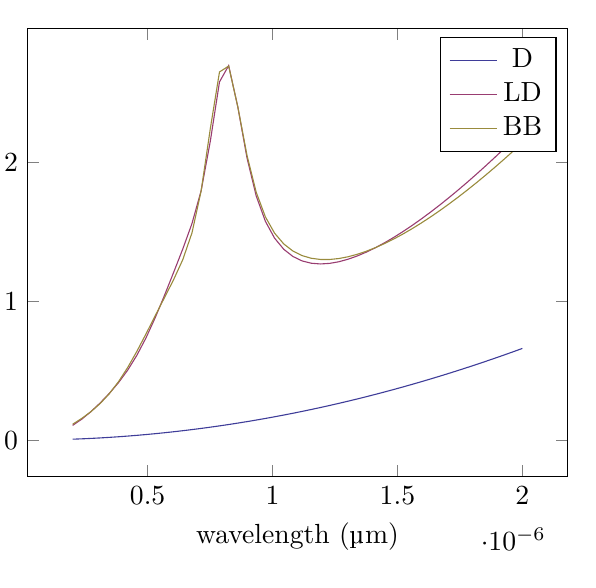
\begin{tikzpicture}[baseline,trim axis left]
			\begin{axis}[xlabel=wavelength (\si{\micro\meter}),ylabel=refractive index $n'$]
				\addplot[color=colora] coordinates {
						(2e-07, 0.00807760888470486)
						(2.3673469387755102e-07, 0.010602454951173408)
						(2.7346938775510205e-07, 0.01363636725397575)
						(3.1020408163265303e-07, 0.017144705945179688)
						(3.4693877551020406e-07, 0.021114246477395685)
						(3.836734693877551e-07, 0.025538872951795185)
						(4.2040816326530607e-07, 0.03041537283493616)
						(4.571428571428571e-07, 0.03574189131121932)
						(4.938775510204081e-07, 0.041517272261194935)
						(5.306122448979591e-07, 0.04774074551716951)
						(5.673469387755102e-07, 0.054411765857012684)
						(6.040816326530612e-07, 0.06152992461077136)
						(6.408163265306121e-07, 0.06909489853140525)
						(6.775510204081632e-07, 0.07710641890995092)
						(7.142857142857142e-07, 0.08556425222416096)
						(7.510204081632653e-07, 0.09446818762693947)
						(7.877551020408163e-07, 0.10381802863463928)
						(8.244897959183672e-07, 0.1136135874718724)
						(8.612244897959183e-07, 0.12385468114256998)
						(8.979591836734693e-07, 0.13454112864873458)
						(9.346938775510204e-07, 0.14567274898877072)
						(9.714285714285713e-07, 0.15724935969510057)
						(1.0081632653061223e-06, 0.16927077575150923)
						(1.0448979591836734e-06, 0.18173680878188936)
						(1.0816326530612245e-06, 0.19464726643569094)
						(1.1183673469387754e-06, 0.2080019519180098)
						(1.1551020408163265e-06, 0.2218006636271086)
						(1.1918367346938776e-06, 0.23604319487285458)
						(1.2285714285714284e-06, 0.25072933365633904)
						(1.2653061224489795e-06, 0.26585886249685203)
						(1.3020408163265306e-06, 0.28143155829507416)
						(1.3387755102040815e-06, 0.2974471922249937)
						(1.3755102040816325e-06, 0.31390552964800156)
						(1.4122448979591836e-06, 0.3308063300449911)
						(1.4489795918367345e-06, 0.3481493469625558)
						(1.4857142857142856e-06, 0.36593432797072684)
						(1.5224489795918367e-06, 0.38416101462993735)
						(1.5591836734693875e-06, 0.40282914246569657)
						(1.5959183673469386e-06, 0.4219384409492959)
						(1.6326530612244897e-06, 0.44148863348392)
						(1.6693877551020408e-06, 0.4614794373949235)
						(1.7061224489795917e-06, 0.48191056392365594)
						(1.7428571428571427e-06, 0.5027817182245544)
						(1.7795918367346938e-06, 0.5240925993645652)
						(1.8163265306122447e-06, 0.5458429003249223)
						(1.8530612244897958e-06, 0.5680323080048089)
						(1.8897959183673469e-06, 0.5906605032265706)
						(1.9265306122448977e-06, 0.6137271607425473)
						(1.963265306122449e-06, 0.6372319492429336)
						(2e-06, 0.6611745313649371)
					};
				\addlegendentry{D}
				\addplot[color=colorb] coordinates {
						(2e-07, 0.10755100665746994)
						(2.3673469387755102e-07, 0.15235734264018785)
						(2.7346938775510205e-07, 0.20667809943510118)
						(3.1020408163265303e-07, 0.26891648528199824)
						(3.4693877551020406e-07, 0.3379181738658425)
						(3.836734693877551e-07, 0.41525440623008475)
						(4.2040816326530607e-07, 0.5051236955234033)
						(4.571428571428571e-07, 0.6119595928148913)
						(4.938775510204081e-07, 0.7382199026544984)
						(5.306122448979591e-07, 0.883091362121921)
						(5.673469387755102e-07, 1.0419877789362308)
						(6.040816326530612e-07, 1.207918146795788)
						(6.408163265306121e-07, 1.3769589114076448)
						(6.775510204081632e-07, 1.5595810431581296)
						(7.142857142857142e-07, 1.7960544282240116)
						(7.510204081632653e-07, 2.1525216296153045)
						(7.877551020408163e-07, 2.5793470514644055)
						(8.244897959183672e-07, 2.696961036284092)
						(8.612244897959183e-07, 2.398012665349278)
						(8.979591836734693e-07, 2.0318602057633264)
						(9.346938775510204e-07, 1.7591590813838829)
						(9.714285714285713e-07, 1.5763746105557603)
						(1.0081632653061223e-06, 1.4552705979541485)
						(1.0448979591836734e-06, 1.3751262173951457)
						(1.0816326530612245e-06, 1.323087782902473)
						(1.1183673469387754e-06, 1.2912052126635658)
						(1.1551020408163265e-06, 1.2743832668183448)
						(1.1918367346938776e-06, 1.2692155118562278)
						(1.2285714285714284e-06, 1.2733331673467998)
						(1.2653061224489795e-06, 1.2850320034706078)
						(1.3020408163265306e-06, 1.3030501820844482)
						(1.3387755102040815e-06, 1.3264305551610356)
						(1.3755102040816325e-06, 1.3544320349039547)
						(1.4122448979591836e-06, 1.386470590902951)
						(1.4489795918367345e-06, 1.422078793866726)
						(1.4857142857142856e-06, 1.4608773576345206)
						(1.5224489795918367e-06, 1.5025546737784359)
						(1.5591836734693875e-06, 1.5468518095454236)
						(1.5959183673469386e-06, 1.5935513257589715)
						(1.6326530612244897e-06, 1.6424688192213979)
						(1.6693877551020408e-06, 1.6934464425887126)
						(1.7061224489795917e-06, 1.7463478818962512)
						(1.7428571428571427e-06, 1.8010544234572592)
						(1.7795918367346938e-06, 1.8574618450054905)
						(1.8163265306122447e-06, 1.9154779374517341)
						(1.8530612244897958e-06, 1.9750205140021049)
						(1.8897959183673469e-06, 2.036015799409814)
						(1.9265306122448977e-06, 2.0983971182378425)
						(1.963265306122449e-06, 2.162103820159757)
						(2e-06, 2.227080394528608)
					};
				\addlegendentry{LD}
				\addplot[color=colorc] coordinates {
						(2e-07, 0.11555063832595779)
						(2.3673469387755102e-07, 0.1579642818131787)
						(2.7346938775510205e-07, 0.20659591765720603)
						(3.1020408163265303e-07, 0.2649171600120164)
						(3.4693877551020406e-07, 0.33600900490993896)
						(3.836734693877551e-07, 0.422119520338419)
						(4.2040816326530607e-07, 0.5241025567045623)
						(4.571428571428571e-07, 0.6404465569688713)
						(4.938775510204081e-07, 0.7667380378192533)
						(5.306122448979591e-07, 0.8968391692749036)
						(5.673469387755102e-07, 1.026126689223065)
						(6.040816326530612e-07, 1.1560657367731466)
						(6.408163265306121e-07, 1.3000586117762924)
						(6.775510204081632e-07, 1.4922807576634578)
						(7.142857142857142e-07, 1.7947753084227291)
						(7.510204081632653e-07, 2.242805955036269)
						(7.877551020408163e-07, 2.6510458621067508)
						(8.244897959183672e-07, 2.6933465950472106)
						(8.612244897959183e-07, 2.399499850648453)
						(8.979591836734693e-07, 2.050421661799598)
						(9.346938775510204e-07, 1.7858098009734074)
						(9.714285714285713e-07, 1.6083409936510173)
						(1.0081632653061223e-06, 1.4912591531632862)
						(1.0448979591836734e-06, 1.4135497216567583)
						(1.0816326530612245e-06, 1.3621942121074528)
						(1.1183673469387754e-06, 1.3293561677858923)
						(1.1551020408163265e-06, 1.310191325143055)
						(1.1918367346938776e-06, 1.3015756893742743)
						(1.2285714285714284e-06, 1.3014026637173501)
						(1.2653061224489795e-06, 1.308190908073835)
						(1.3020408163265306e-06, 1.3208591809342896)
						(1.3387755102040815e-06, 1.3385924522985266)
						(1.3755102040816325e-06, 1.3607593377160798)
						(1.4122448979591836e-06, 1.3868593312236905)
						(1.4489795918367345e-06, 1.4164879186448542)
						(1.4857142857142856e-06, 1.4493127721437409)
						(1.5224489795918367e-06, 1.485057029516018)
						(1.5591836734693875e-06, 1.523487239036945)
						(1.5959183673469386e-06, 1.5644044632429954)
						(1.6326530612244897e-06, 1.6076375773825118)
						(1.6693877551020408e-06, 1.6530381291290657)
						(1.7061224489795917e-06, 1.7004763331264967)
						(1.7428571428571427e-06, 1.7498379065768048)
						(1.7795918367346938e-06, 1.8010215390751525)
						(1.8163265306122447e-06, 1.853936848216653)
						(1.8530612244897958e-06, 1.908502712420619)
						(1.8897959183673469e-06, 1.9646459002828731)
						(1.9265306122448977e-06, 2.0222999355743805)
						(1.963265306122449e-06, 2.0814041513255757)
						(2e-06, 2.14190289695206)
					};
				\addlegendentry{BB}
			\end{axis}
		\end{tikzpicture}%
		\\
		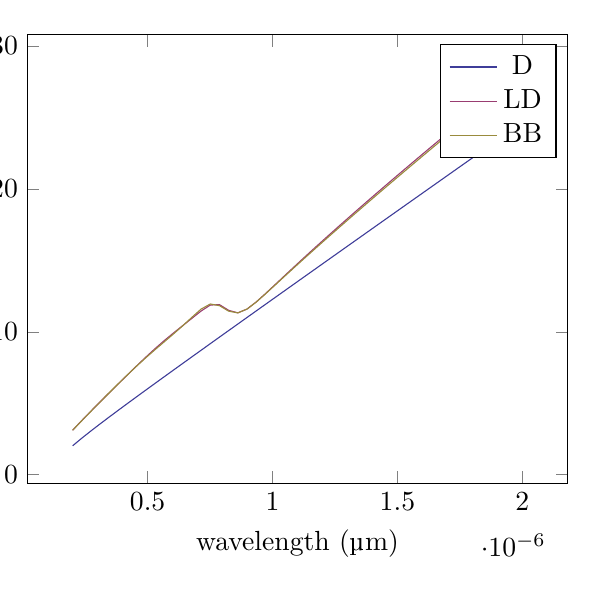
\begin{tikzpicture}[baseline,trim axis left]
			\begin{axis}[xlabel=wavelength (\si{\micro\meter}),ylabel=refractive index $n''$]
				\addplot[color=colora] coordinates {
						(2e-07, 2.026708845596848)
						(2.3673469387755102e-07, 2.5606691947802362)
						(2.7346938775510205e-07, 3.0689510066720818)
						(3.1020408163265303e-07, 3.5625551232260753)
						(3.4693877551020406e-07, 4.0468488503990905)
						(3.836734693877551e-07, 4.5248155492285305)
						(4.2040816326530607e-07, 4.998263490078203)
						(4.571428571428571e-07, 5.468359301459567)
						(4.938775510204081e-07, 5.935892228124918)
						(5.306122448979591e-07, 6.401416579890191)
						(5.673469387755102e-07, 6.865333668666994)
						(6.040816326530612e-07, 7.327941438633974)
						(6.408163265306121e-07, 7.789465825537508)
						(6.775510204081632e-07, 8.2500812832407)
						(7.142857142857142e-07, 8.709924628466966)
						(7.510204081632653e-07, 9.169104623017425)
						(7.877551020408163e-07, 9.62770875667283)
						(8.244897959183672e-07, 10.085808144530878)
						(8.612244897959183e-07, 10.543461125588793)
						(8.979591836734693e-07, 11.000715948836893)
						(9.346938775510204e-07, 11.457612806765976)
						(9.714285714285713e-07, 11.91418539464107)
						(1.0081632653061223e-06, 12.370462120122552)
						(1.0448979591836734e-06, 12.82646705166631)
						(1.0816326530612245e-06, 13.282220669401553)
						(1.1183673469387754e-06, 13.737740464988669)
						(1.1551020408163265e-06, 14.193041424826918)
						(1.1918367346938776e-06, 14.648136422304937)
						(1.2285714285714284e-06, 15.103036538503998)
						(1.2653061224489795e-06, 15.557751326161412)
						(1.3020408163265306e-06, 16.012289028293335)
						(1.3387755102040815e-06, 16.466656760327638)
						(1.3755102040816325e-06, 16.920860662673263)
						(1.4122448979591836e-06, 17.37490602918737)
						(1.4489795918367345e-06, 17.828797415876426)
						(1.4857142857142856e-06, 18.282538733297056)
						(1.5224489795918367e-06, 18.736133325443866)
						(1.5591836734693875e-06, 19.18958403737918)
						(1.5959183673469386e-06, 19.642893273438986)
						(1.6326530612244897e-06, 20.096063047515283)
						(1.6693877551020408e-06, 20.549095026647688)
						(1.7061224489795917e-06, 21.001990568942723)
						(1.7428571428571427e-06, 21.454750756665288)
						(1.7795918367346938e-06, 21.907376425206305)
						(1.8163265306122447e-06, 22.3598681885152)
						(1.8530612244897958e-06, 22.812226461491935)
						(1.8897959183673469e-06, 23.264451479755415)
						(1.9265306122448977e-06, 23.716543317141134)
						(1.963265306122449e-06, 24.168501901227728)
						(2e-06, 24.62032702714737)
					};
				\addlegendentry{D}
				\addplot[color=colorb] coordinates {
						(2e-07, 3.116786873861261)
						(2.3673469387755102e-07, 3.796649735168536)
						(2.7346938775510205e-07, 4.457393256083114)
						(3.1020408163265303e-07, 5.103858231843916)
						(3.4693877551020406e-07, 5.741218607893461)
						(3.836734693877551e-07, 6.374661246761554)
						(4.2040816326530607e-07, 7.005863288365583)
						(4.571428571428571e-07, 7.631335412719943)
						(4.938775510204081e-07, 8.24358040187064)
						(5.306122448979591e-07, 8.833459541757408)
						(5.673469387755102e-07, 9.393645164276139)
						(6.040816326530612e-07, 9.923554311968488)
						(6.408163265306121e-07, 10.433776818076074)
						(6.775510204081632e-07, 10.943261501099839)
						(7.142857142857142e-07, 11.453962332661845)
						(7.510204081632653e-07, 11.869323290492003)
						(7.877551020408163e-07, 11.898230489518506)
						(8.244897959183672e-07, 11.500791179790347)
						(8.612244897959183e-07, 11.32497458599406)
						(8.979591836734693e-07, 11.590470792464624)
						(9.346938775510204e-07, 12.085758314069635)
						(9.714285714285713e-07, 12.661980394412662)
						(1.0081632653061223e-06, 13.261276851342839)
						(1.0448979591836734e-06, 13.863835925562556)
						(1.0816326530612245e-06, 14.463070518858833)
						(1.1183673469387754e-06, 15.05694947629732)
						(1.1551020408163265e-06, 15.64505074320759)
						(1.1918367346938776e-06, 16.227523569976587)
						(1.2285714285714284e-06, 16.804706463285655)
						(1.2653061224489795e-06, 17.376981941210023)
						(1.3020408163265306e-06, 17.944721213948743)
						(1.3387755102040815e-06, 18.508264467633335)
						(1.3755102040816325e-06, 19.067915611884374)
						(1.4122448979591836e-06, 19.623942891219848)
						(1.4489795918367345e-06, 20.176581738188435)
						(1.4857142857142856e-06, 20.726038311593094)
						(1.5224489795918367e-06, 21.272493053214404)
						(1.5591836734693875e-06, 21.81610399125087)
						(1.5959183673469386e-06, 22.357009696712485)
						(1.6326530612244897e-06, 22.895331878996988)
						(1.6693877551020408e-06, 23.43117764143597)
						(1.7061224489795917e-06, 23.964641430801993)
						(1.7428571428571427e-06, 24.495806717960456)
						(1.7795918367346938e-06, 25.024747445491176)
						(1.8163265306122447e-06, 25.551529274853245)
						(1.8530612244897958e-06, 26.076210661818273)
						(1.8897959183673469e-06, 26.59884378506549)
						(1.9265306122448977e-06, 27.119475349292866)
						(1.963265306122449e-06, 27.63814728105248)
						(2e-06, 28.15489733278403)
					};
				\addlegendentry{LD}
				\addplot[color=colorc] coordinates {
						(2e-07, 3.1132616264282134)
						(2.3673469387755102e-07, 3.785245803658046)
						(2.7346938775510205e-07, 4.444490813530607)
						(3.1020408163265303e-07, 5.0973804800382805)
						(3.4693877551020406e-07, 5.744664295489672)
						(3.836734693877551e-07, 6.383798018886378)
						(4.2040816326530607e-07, 7.009838035010825)
						(4.571428571428571e-07, 7.6167370302802)
						(4.938775510204081e-07, 8.200135723575178)
						(5.306122448979591e-07, 8.76096202435741)
						(5.673469387755102e-07, 9.307680713956145)
						(6.040816326530612e-07, 9.855639120396077)
						(6.408163265306121e-07, 10.422772006323465)
						(6.775510204081632e-07, 11.016635318007069)
						(7.142857142857142e-07, 11.589879947020085)
						(7.510204081632653e-07, 11.944185871699723)
						(7.877551020408163e-07, 11.825942627886613)
						(8.244897959183672e-07, 11.442538082262619)
						(8.612244897959183e-07, 11.319567108730515)
						(8.979591836734693e-07, 11.587892849688282)
						(9.346938775510204e-07, 12.075560148662007)
						(9.714285714285713e-07, 12.643318415562758)
						(1.0081632653061223e-06, 13.232610571673037)
						(1.0448979591836734e-06, 13.823757960963109)
						(1.0816326530612245e-06, 14.410946146369538)
						(1.1183673469387754e-06, 14.992880368771463)
						(1.1551020408163265e-06, 15.569649405657689)
						(1.1918367346938776e-06, 16.141699786422645)
						(1.2285714285714284e-06, 16.70951152229932)
						(1.2653061224489795e-06, 17.273507143637058)
						(1.3020408163265306e-06, 17.834036701475412)
						(1.3387755102040815e-06, 18.39138530837468)
						(1.3755102040816325e-06, 18.94578534747999)
						(1.4122448979591836e-06, 19.49742780858861)
						(1.4489795918367345e-06, 20.04647143693907)
						(1.4857142857142856e-06, 20.593049740357436)
						(1.5224489795918367e-06, 21.13727625526628)
						(1.5591836734693875e-06, 21.679248493098537)
						(1.5959183673469386e-06, 22.21905091596593)
						(1.6326530612244897e-06, 22.75675720602891)
						(1.6693877551020408e-06, 23.292432021325137)
						(1.7061224489795917e-06, 23.82613237608701)
						(1.7428571428571427e-06, 24.357908743762376)
						(1.7795918367346938e-06, 24.88780595265425)
						(1.8163265306122447e-06, 25.415863924197716)
						(1.8530612244897958e-06, 25.942118289951388)
						(1.8897959183673469e-06, 26.46660091360064)
						(1.9265306122448977e-06, 26.98934033737956)
						(1.963265306122449e-06, 27.510362167430046)
						(2e-06, 28.029689409118554)
					};
				\addlegendentry{BB}
			\end{axis}
		\end{tikzpicture}%
		\\
	\end{tabular}
	\caption{Complex permittivity $\epsilon = \epsilon' + \mi \epsilon''$ and refractive index $n = n' + \mi n''$ for Al based on the Drude (D), Lorentz-Drude (LD), and Brendel-Bormann (BB) models.}
\end{figure}
\clearpage
\newpage
\subsection{Au}
\begin{figure}[h!]
	\centering
	\begin{tabular}{l}
		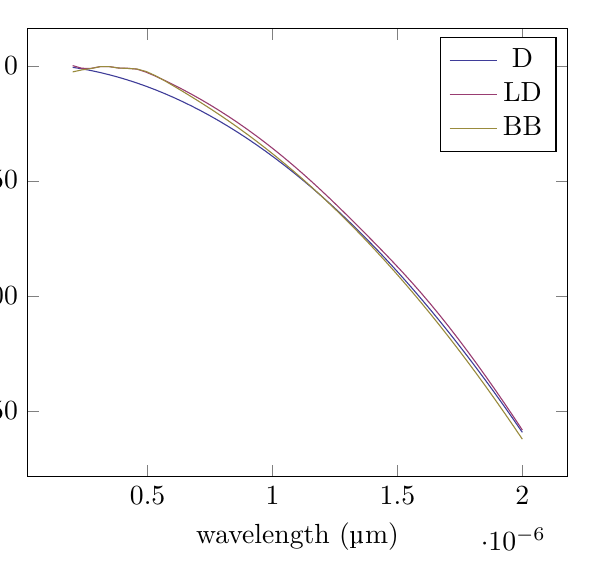
\begin{tikzpicture}[baseline,trim axis left]
			\begin{axis}[xlabel=wavelength (\si{\micro\meter}),ylabel=permittivity $\epsilon'$]
				\addplot[color=colora] coordinates {
						(2e-07, -0.6124440870620205)
						(2.3673469387755102e-07, -1.2591015845055509)
						(2.7346938775510205e-07, -2.0144945732194186)
						(3.1020408163265303e-07, -2.878600708855132)
						(3.4693877551020406e-07, -3.8513944341696016)
						(3.836734693877551e-07, -4.932846980914447)
						(4.2040816326530607e-07, -6.122926371962317)
						(4.571428571428571e-07, -7.421597423669896)
						(4.938775510204081e-07, -8.828821748477278)
						(5.306122448979591e-07, -10.34455775774336)
						(5.673469387755102e-07, -11.968760664816866)
						(6.040816326530612e-07, -13.701382488342535)
						(6.408163265306121e-07, -15.542372055802097)
						(6.775510204081632e-07, -17.49167500728948)
						(7.142857142857142e-07, -19.549233799519747)
						(7.510204081632653e-07, -21.714987710071235)
						(7.877551020408163e-07, -23.98887284186028)
						(8.244897959183672e-07, -26.37082212784798)
						(8.612244897959183e-07, -28.86076533597822)
						(8.979591836734693e-07, -31.458629074346355)
						(9.346938775510204e-07, -34.16433679659801)
						(9.714285714285713e-07, -36.97780880755685)
						(1.0081632653061223e-06, -39.89896226908101)
						(1.0448979591836734e-06, -42.927711206147016)
						(1.0816326530612245e-06, -46.06396651316063)
						(1.1183673469387754e-06, -49.307635960493464)
						(1.1551020408163265e-06, -52.65862420124499)
						(1.1918367346938776e-06, -56.11683277822824)
						(1.2285714285714284e-06, -59.682160131179)
						(1.2653061224489795e-06, -63.354501604187135)
						(1.3020408163265306e-06, -67.13374945334905)
						(1.3387755102040815e-06, -71.01979285464026)
						(1.3755102040816325e-06, -75.01251791200723)
						(1.4122448979591836e-06, -79.11180766567686)
						(1.4489795918367345e-06, -83.31754210068314)
						(1.4857142857142856e-06, -87.6295981556094)
						(1.5224489795918367e-06, -92.04784973154499)
						(1.5591836734693875e-06, -96.57216770125527)
						(1.5959183673469386e-06, -101.20241991856378)
						(1.6326530612244897e-06, -105.93847122794516)
						(1.6693877551020408e-06, -110.78018347432737)
						(1.7061224489795917e-06, -115.72741551310257)
						(1.7428571428571427e-06, -120.78002322034435)
						(1.7795918367346938e-06, -125.93785950323064)
						(1.8163265306122447e-06, -131.20077431067068)
						(1.8530612244897958e-06, -136.5686146441349)
						(1.8897959183673469e-06, -142.04122456868532)
						(1.9265306122448977e-06, -147.6184452242063)
						(1.963265306122449e-06, -153.3001148368336)
						(2e-06, -159.08606873057946)
					};
				\addlegendentry{D}
				\addplot[color=colorb] coordinates {
						(2e-07, 0.13724980083673177)
						(2.3673469387755102e-07, -1.0316335820904454)
						(2.7346938775510205e-07, -1.0785730911790823)
						(3.1020408163265303e-07, -0.32139109844480984)
						(3.4693877551020406e-07, -0.3059743533560173)
						(3.836734693877551e-07, -0.9205243107532715)
						(4.2040816326530607e-07, -1.0361088367581495)
						(4.571428571428571e-07, -1.4044940404284638)
						(4.938775510204081e-07, -2.71145605081699)
						(5.306122448979591e-07, -4.409012183837599)
						(5.673469387755102e-07, -6.258729570910543)
						(6.040816326530612e-07, -8.209485035235657)
						(6.408163265306121e-07, -10.254535872305912)
						(6.775510204081632e-07, -12.396255855423291)
						(7.142857142857142e-07, -14.638334496211437)
						(7.510204081632653e-07, -16.98410729288121)
						(7.877551020408163e-07, -19.436297340115978)
						(8.244897959183672e-07, -21.997068906765936)
						(8.612244897959183e-07, -24.66812296383482)
						(8.979591836734693e-07, -27.450768294812214)
						(9.346938775510204e-07, -30.345952473858638)
						(9.714285714285713e-07, -33.354247317950744)
						(1.0081632653061223e-06, -36.47578253406536)
						(1.0448979591836734e-06, -39.710117440206695)
						(1.0816326530612245e-06, -43.056037135612954)
						(1.1183673469387754e-06, -46.51125974276465)
						(1.1551020408163265e-06, -50.07205162074985)
						(1.1918367346938776e-06, -53.732779227016856)
						(1.2285714285714284e-06, -57.485496834356006)
						(1.2653061224489795e-06, -61.31979458767363)
						(1.3020408163265306e-06, -65.22329921808499)
						(1.3387755102040815e-06, -69.18333266704241)
						(1.3755102040816325e-06, -73.19005468632464)
						(1.4122448979591836e-06, -77.240658923633)
						(1.4489795918367345e-06, -81.34294911931384)
						(1.4857142857142856e-06, -85.51586289609517)
						(1.5224489795918367e-06, -89.78559024890014)
						(1.5591836734693875e-06, -94.17870687802456)
						(1.5959183673469386e-06, -98.71580002152633)
						(1.6326530612244897e-06, -103.40836895133995)
						(1.6693877551020408e-06, -108.25929354380743)
						(1.7061224489795917e-06, -113.26533136193986)
						(1.7428571428571427e-06, -118.41992455158265)
						(1.7795918367346938e-06, -123.71535471065097)
						(1.8163265306122447e-06, -129.14403371867664)
						(1.8530612244897958e-06, -134.69910131964843)
						(1.8897959183673469e-06, -140.374585899983)
						(1.9265306122448977e-06, -146.16533671547964)
						(1.963265306122449e-06, -152.06686049404675)
						(2e-06, -158.07513491191617)
					};
				\addlegendentry{LD}
				\addplot[color=colorc] coordinates {
						(2e-07, -2.6079132898496544)
						(2.3673469387755102e-07, -1.7427284926134858)
						(2.7346938775510205e-07, -1.135945664078756)
						(3.1020408163265303e-07, -0.33576677741036454)
						(3.4693877551020406e-07, -0.33008315153089507)
						(3.836734693877551e-07, -0.9166108095677457)
						(4.2040816326530607e-07, -1.0934293445980483)
						(4.571428571428571e-07, -1.3481116480664497)
						(4.938775510204081e-07, -2.411486764831185)
						(5.306122448979591e-07, -4.207796495696715)
						(5.673469387755102e-07, -6.381609412323868)
						(6.040816326530612e-07, -8.703779267322673)
						(6.408163265306121e-07, -11.08975638208813)
						(6.775510204081632e-07, -13.524918942748032)
						(7.142857142857142e-07, -16.01657689115116)
						(7.510204081632653e-07, -18.575199561118495)
						(7.877551020408163e-07, -21.20932023484167)
						(8.244897959183672e-07, -23.9250238082325)
						(8.612244897959183e-07, -26.726521092978125)
						(8.979591836734693e-07, -29.61676854492506)
						(9.346938775510204e-07, -32.597919509415036)
						(9.714285714285713e-07, -35.67161638130457)
						(1.0081632653061223e-06, -38.83917144209524)
						(1.0448979591836734e-06, -42.101676971638135)
						(1.0816326530612245e-06, -45.460072103434214)
						(1.1183673469387754e-06, -48.91518362234221)
						(1.1551020408163265e-06, -52.46775115560391)
						(1.1918367346938776e-06, -56.11844303851788)
						(1.2285714285714284e-06, -59.86786661710712)
						(1.2653061224489795e-06, -63.716575238283326)
						(1.3020408163265306e-06, -67.66507327082098)
						(1.3387755102040815e-06, -71.71381995528624)
						(1.3755102040816325e-06, -75.86323255323822)
						(1.4122448979591836e-06, -80.11368906922485)
						(1.4489795918367345e-06, -84.46553070157783)
						(1.4857142857142856e-06, -88.91906410853157)
						(1.5224489795918367e-06, -93.47456353578596)
						(1.5591836734693875e-06, -98.13227282874576)
						(1.5959183673469386e-06, -102.89240734022864)
						(1.6326530612244897e-06, -107.75515573813325)
						(1.6693877551020408e-06, -112.72068171477142)
						(1.7061224489795917e-06, -117.78912559871598)
						(1.7428571428571427e-06, -122.9606058701496)
						(1.7795918367346938e-06, -128.23522058128177)
						(1.8163265306122447e-06, -133.61304868411247)
						(1.8530612244897958e-06, -139.09415126850675)
						(1.8897959183673469e-06, -144.67857271411688)
						(1.9265306122448977e-06, -150.36634176013166)
						(1.963265306122449e-06, -156.1574724971304)
						(2e-06, -162.05196528549448)
					};
				\addlegendentry{BB}
			\end{axis}
		\end{tikzpicture}%
		\\
		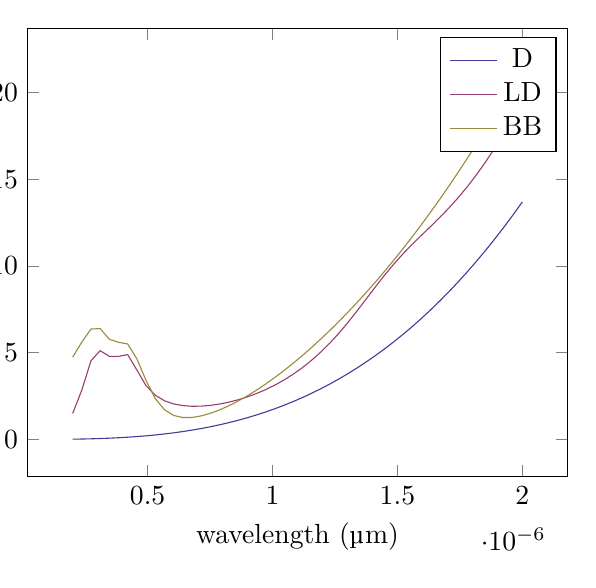
\begin{tikzpicture}[baseline,trim axis left]
			\begin{axis}[xlabel=wavelength (\si{\micro\meter}),ylabel=permittivity $\epsilon''$]
				\addplot[color=colora] coordinates {
						(2e-07, 0.01378555294856072)
						(2.3673469387755102e-07, 0.022861630455046047)
						(2.7346938775510205e-07, 0.03523974488248825)
						(3.1020408163265303e-07, 0.05143184588364701)
						(3.4693877551020406e-07, 0.07194969511133043)
						(3.836734693877551e-07, 0.09730484102314653)
						(4.2040816326530607e-07, 0.12800859370831505)
						(4.571428571428571e-07, 0.1645719997391384)
						(4.938775510204081e-07, 0.2075058170497265)
						(5.306122448979591e-07, 0.2573204898445665)
						(5.673469387755102e-07, 0.31452612353952164)
						(6.040816326530612e-07, 0.37963245973783727)
						(6.408163265306121e-07, 0.4531488512437293)
						(6.775510204081632e-07, 0.5355842371161191)
						(7.142857142857142e-07, 0.6274471177650759)
						(7.510204081632653e-07, 0.7292455300935146)
						(7.877551020408163e-07, 0.8414870226866985)
						(8.244897959183672e-07, 0.9646786310520771)
						(8.612244897959183e-07, 1.0993268529119877)
						(8.979591836734693e-07, 1.245937623551732)
						(9.346938775510204e-07, 1.4050162912255504)
						(9.714285714285713e-07, 1.5770675926229678)
						(1.0081632653061223e-06, 1.7625956283980215)
						(1.0448979591836734e-06, 1.9621038387638228)
						(1.0816326530612245e-06, 2.1760949791549424)
						(1.1183673469387754e-06, 2.4050710959600368)
						(1.1551020408163265e-06, 2.649533502327206)
						(1.1918367346938776e-06, 2.9099827540444427)
						(1.2285714285714284e-06, 3.1869186254976514)
						(1.2653061224489795e-06, 3.480840085708597)
						(1.3020408163265306e-06, 3.792245274455182)
						(1.3387755102040815e-06, 4.121631478476422)
						(1.3755102040816325e-06, 4.469495107764487)
						(1.4122448979591836e-06, 4.836331671946126)
						(1.4489795918367345e-06, 5.222635756755815)
						(1.4857142857142856e-06, 5.628901000602973)
						(1.5224489795918367e-06, 6.0556200712354595)
						(1.5591836734693875e-06, 6.5032846425017095)
						(1.5959183673469386e-06, 6.972385371213721)
						(1.6326530612244897e-06, 7.463411874113166)
						(1.6693877551020408e-06, 7.976852704942799)
						(1.7061224489795917e-06, 8.513195331625468)
						(1.7428571428571427e-06, 9.0729261135528)
						(1.7795918367346938e-06, 9.656530278985791)
						(1.8163265306122447e-06, 10.264491902569466)
						(1.8530612244897958e-06, 10.897293882963732)
						(1.8897959183673469e-06, 11.555417920592458)
						(1.9265306122448977e-06, 12.239344495512968)
						(1.963265306122449e-06, 12.949552845408052)
						(2e-06, 13.686520943702334)
					};
				\addlegendentry{D}
				\addplot[color=colorb] coordinates {
						(2e-07, 1.4956409650239693)
						(2.3673469387755102e-07, 2.8446555083130995)
						(2.7346938775510205e-07, 4.536361819952192)
						(3.1020408163265303e-07, 5.116870925793828)
						(3.4693877551020406e-07, 4.7855625923183505)
						(3.836734693877551e-07, 4.78683662136402)
						(4.2040816326530607e-07, 4.885628317932741)
						(4.571428571428571e-07, 3.9992228404186534)
						(4.938775510204081e-07, 3.096191547609063)
						(5.306122448979591e-07, 2.5471206724441298)
						(5.673469387755102e-07, 2.229480297777576)
						(6.040816326530612e-07, 2.0468277341576733)
						(6.408163265306121e-07, 1.9493124608876582)
						(6.775510204081632e-07, 1.9110500575696783)
						(7.142857142857142e-07, 1.9179061868245122)
						(7.510204081632653e-07, 1.9618662814793255)
						(7.877551020408163e-07, 2.038359077567133)
						(8.244897959183672e-07, 2.144910549543185)
						(8.612244897959183e-07, 2.2804332597106898)
						(8.979591836734693e-07, 2.4448403338344216)
						(9.346938775510204e-07, 2.638836119901088)
						(9.714285714285713e-07, 2.863807467234658)
						(1.0081632653061223e-06, 3.121771344796926)
						(1.0448979591836734e-06, 3.4153461525723445)
						(1.0816326530612245e-06, 3.7477129282885304)
						(1.1183673469387754e-06, 4.122520629030138)
						(1.1551020408163265e-06, 4.543666965018103)
						(1.1918367346938776e-06, 5.0148555235097)
						(1.2285714285714284e-06, 5.538803927383396)
						(1.2653061224489795e-06, 6.115992379706067)
						(1.3020408163265306e-06, 6.742968207423328)
						(1.3387755102040815e-06, 7.410548707975032)
						(1.3755102040816325e-06, 8.102792210028223)
						(1.4122448979591836e-06, 8.79803507222549)
						(1.4489795918367345e-06, 9.472933606897978)
						(1.4857142857142856e-06, 10.1088058723178)
						(1.5224489795918367e-06, 10.6974787778249)
						(1.5591836734693875e-06, 11.243440821504002)
						(1.5959183673469386e-06, 11.761338183056225)
						(1.6326530612244897e-06, 12.270759742564444)
						(1.6693877551020408e-06, 12.791221076535223)
						(1.7061224489795917e-06, 13.339089041727384)
						(1.7428571428571427e-06, 13.92656871835008)
						(1.7795918367346938e-06, 14.562023872542081)
						(1.8163265306122447e-06, 15.25084940514455)
						(1.8530612244897958e-06, 15.996396717451612)
						(1.8897959183673469e-06, 16.800732699041475)
						(1.9265306122448977e-06, 17.665183296365313)
						(1.963265306122449e-06, 18.59068751392105)
						(2e-06, 19.57800803540715)
					};
				\addlegendentry{LD}
				\addplot[color=colorc] coordinates {
						(2e-07, 4.743844285697897)
						(2.3673469387755102e-07, 5.609360205618437)
						(2.7346938775510205e-07, 6.360905065524743)
						(3.1020408163265303e-07, 6.388982980739583)
						(3.4693877551020406e-07, 5.769836321254253)
						(3.836734693877551e-07, 5.5975729801271905)
						(4.2040816326530607e-07, 5.501799277039835)
						(4.571428571428571e-07, 4.6444084198808575)
						(4.938775510204081e-07, 3.3962788100066628)
						(5.306122448979591e-07, 2.3594794319294783)
						(5.673469387755102e-07, 1.7129660315791286)
						(6.040816326530612e-07, 1.3834010169966606)
						(6.408163265306121e-07, 1.2602537917307235)
						(6.775510204081632e-07, 1.2657167439607457)
						(7.142857142857142e-07, 1.3551810078742443)
						(7.510204081632653e-07, 1.5045167339319772)
						(7.877551020408163e-07, 1.7004311480800345)
						(8.244897959183672e-07, 1.935115918125386)
						(8.612244897959183e-07, 2.203578761047619)
						(8.979591836734693e-07, 2.502355406658104)
						(9.346938775510204e-07, 2.828882386659837)
						(9.714285714285713e-07, 3.1811800346386416)
						(1.0081632653061223e-06, 3.557682314169244)
						(1.0448979591836734e-06, 3.957137982139722)
						(1.0816326530612245e-06, 4.378547832480757)
						(1.1183673469387754e-06, 4.821121199979041)
						(1.1551020408163265e-06, 5.284243468010818)
						(1.1918367346938776e-06, 5.7674503847299)
						(1.2285714285714284e-06, 6.270406962497942)
						(1.2653061224489795e-06, 6.792889714617063)
						(1.3020408163265306e-06, 7.334771482799015)
						(1.3387755102040815e-06, 7.896008371182828)
						(1.3755102040816325e-06, 8.476628446017926)
						(1.4122448979591836e-06, 9.076721942668271)
						(1.4489795918367345e-06, 9.696432772607281)
						(1.4857142857142856e-06, 10.335951157371124)
						(1.5224489795918367e-06, 10.995507241561143)
						(1.5591836734693875e-06, 11.675365556787415)
						(1.5959183673469386e-06, 12.375820224898163)
						(1.6326530612244897e-06, 13.09719080296662)
						(1.6693877551020408e-06, 13.839818684851519)
						(1.7061224489795917e-06, 14.604063985018668)
						(1.7428571428571427e-06, 15.39030283990316)
						(1.7795918367346938e-06, 16.198925070546395)
						(1.8163265306122447e-06, 17.03033215767527)
						(1.8530612244897958e-06, 17.884935486905373)
						(1.8897959183673469e-06, 18.763154827442147)
						(1.9265306122448977e-06, 19.66541701261329)
						(1.963265306122449e-06, 20.592154794874844)
						(2e-06, 21.543805851669305)
					};
				\addlegendentry{BB}
			\end{axis}
		\end{tikzpicture}%
		\\
		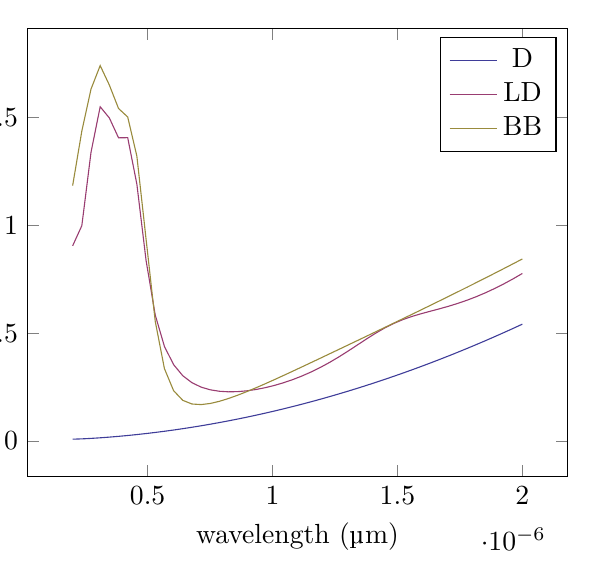
\begin{tikzpicture}[baseline,trim axis left]
			\begin{axis}[xlabel=wavelength (\si{\micro\meter}),ylabel=refractive index $n'$]
				\addplot[color=colora] coordinates {
						(2e-07, 0.008807111047271056)
						(2.3673469387755102e-07, 0.010186592293689144)
						(2.7346938775510205e-07, 0.01241375297018575)
						(3.1020408163265303e-07, 0.015156330742437347)
						(3.4693877551020406e-07, 0.01833036106343869)
						(3.836734693877551e-07, 0.021904558766988578)
						(4.2040816326530607e-07, 0.0258646072752396)
						(4.571428571428571e-07, 0.030203033567835796)
						(4.938775510204081e-07, 0.034915552927982985)
						(5.306122448979591e-07, 0.039999524303617986)
						(5.673469387755102e-07, 0.045453220071095264)
						(6.040816326530612e-07, 0.05127545035008038)
						(6.408163265306121e-07, 0.05746535647948646)
						(6.775510204081632e-07, 0.064022291246247)
						(7.142857142857142e-07, 0.07094574628839917)
						(7.510204081632653e-07, 0.07823530642648499)
						(7.877551020408163e-07, 0.0858906200092469)
						(8.244897959183672e-07, 0.09391137912329087)
						(8.612244897959183e-07, 0.10229730606548813)
						(8.979591836734693e-07, 0.11104814389960463)
						(9.346938775510204e-07, 0.12016364973938104)
						(9.714285714285713e-07, 0.12964358989047606)
						(1.0081632653061223e-06, 0.1394877362838591)
						(1.0448979591836734e-06, 0.1496958638216242)
						(1.0816326530612245e-06, 0.1602677483776921)
						(1.1183673469387754e-06, 0.171203165274974)
						(1.1551020408163265e-06, 0.18250188811397214)
						(1.1918367346938776e-06, 0.19416368786329125)
						(1.2285714285714284e-06, 0.20618833214806626)
						(1.2653061224489795e-06, 0.21857558468879457)
						(1.3020408163265306e-06, 0.2313252048562924)
						(1.3387755102040815e-06, 0.24443694731637217)
						(1.3755102040816325e-06, 0.25791056174512617)
						(1.4122448979591836e-06, 0.27174579259963555)
						(1.4489795918367345e-06, 0.28594237893278174)
						(1.4857142857142856e-06, 0.3005000542435581)
						(1.5224489795918367e-06, 0.3154185463556841)
						(1.5591836734693875e-06, 0.33069757731939636)
						(1.5959183673469386e-06, 0.3463368633320705)
						(1.6326530612244897e-06, 0.3623361146742997)
						(1.6693877551020408e-06, 0.3786950356588259)
						(1.7061224489795917e-06, 0.39541332458993883)
						(1.7428571428571427e-06, 0.4124906737318886)
						(1.7795918367346938e-06, 0.4299267692846302)
						(1.8163265306122447e-06, 0.4477212913659146)
						(1.8530612244897958e-06, 0.4658739139986474)
						(1.8897959183673469e-06, 0.48438430510288943)
						(1.9265306122448977e-06, 0.5032521264916152)
						(1.963265306122449e-06, 0.5224770338699256)
						(2e-06, 0.5420586768371869)
					};
				\addlegendentry{D}
				\addplot[color=colorb] coordinates {
						(2e-07, 0.905310729351851)
						(2.3673469387755102e-07, 0.9985764142731249)
						(2.7346938775510205e-07, 1.338702315633979)
						(3.1020408163265303e-07, 1.5500908349635405)
						(3.4693877551020406e-07, 1.4982255835993954)
						(3.836734693877551e-07, 1.4060616503181886)
						(4.2040816326530607e-07, 1.4068007065169357)
						(4.571428571428571e-07, 1.190416617481107)
						(4.938775510204081e-07, 0.8379057865004066)
						(5.306122448979591e-07, 0.584322210845525)
						(5.673469387755102e-07, 0.43888266078232163)
						(6.040816326530612e-07, 0.35448247829302476)
						(6.408163265306121e-07, 0.30301062204040863)
						(6.775510204081632e-07, 0.2705938674911046)
						(7.142857142857142e-07, 0.25010684685830303)
						(7.510204081632653e-07, 0.2376278256143967)
						(7.877551020408163e-07, 0.23086032458622024)
						(8.244897959183672e-07, 0.22839282386434515)
						(8.612244897959183e-07, 0.22932788387115507)
						(8.979591836734693e-07, 0.2330847807034149)
						(9.346938775510204e-07, 0.23928897679101788)
						(9.714285714285713e-07, 0.24770749567546946)
						(1.0081632653061223e-06, 0.25820951125002295)
						(1.0448979591836734e-06, 0.2707407855866582)
						(1.0816326530612245e-06, 0.2853048518559422)
						(1.1183673469387754e-06, 0.3019454965734636)
						(1.1551020408163265e-06, 0.3207252612215976)
						(1.1918367346938776e-06, 0.3416940803772931)
						(1.2285714285714284e-06, 0.3648418261683389)
						(1.2653061224489795e-06, 0.3900304883015105)
						(1.3020408163265306e-06, 0.4169095359397804)
						(1.3387755102040815e-06, 0.4448354927556877)
						(1.3755102040816325e-06, 0.472842324257376)
						(1.4122448979591836e-06, 0.4997258144235136)
						(1.4489795918367345e-06, 0.5242784543756518)
						(1.4857142857142856e-06, 0.5456220153268481)
						(1.5224489795918367e-06, 0.5634839634270618)
						(1.5591836734693875e-06, 0.5782601410320644)
						(1.5959183673469386e-06, 0.5908358890280877)
						(1.6326530612244897e-06, 0.6022866114097706)
						(1.6693877551020408e-06, 0.6136143307348517)
						(1.7061224489795917e-06, 0.6256027302978722)
						(1.7428571428571427e-06, 0.6387851185504552)
						(1.7795918367346938e-06, 0.6534790854464092)
						(1.8163265306122447e-06, 0.6698440842913972)
						(1.8530612244897958e-06, 0.6879362999263768)
						(1.8897959183673469e-06, 0.7077510059985891)
						(1.9265306122448977e-06, 0.7292514853623273)
						(1.963265306122449e-06, 0.7523870482063938)
						(2e-06, 0.7771032868901614)
					};
				\addlegendentry{LD}
				\addplot[color=colorc] coordinates {
						(2e-07, 1.184381897028384)
						(2.3673469387755102e-07, 1.4372045618638256)
						(2.7346938775510205e-07, 1.631807786099739)
						(3.1020408163265303e-07, 1.740981485773744)
						(3.4693877551020406e-07, 1.6506343057925608)
						(3.836734693877551e-07, 1.541997712908171)
						(4.2040816326530607e-07, 1.5026596357495186)
						(4.571428571428571e-07, 1.320605113472656)
						(4.938775510204081e-07, 0.9364410645982637)
						(5.306122448979591e-07, 0.5551493604715337)
						(5.673469387755102e-07, 0.33608094887054407)
						(6.040816326530612e-07, 0.23372519999153743)
						(6.408163265306121e-07, 0.1889162461295187)
						(6.775510204081632e-07, 0.17189581585240213)
						(7.142857142857142e-07, 0.16915890175546575)
						(7.510204081632653e-07, 0.1743994115326498)
						(7.877551020408163e-07, 0.18446652766317506)
						(8.244897959183672e-07, 0.19764986649062757)
						(8.612244897959183e-07, 0.21294099022975352)
						(8.979591836734693e-07, 0.22970140611092213)
						(9.346938775510204e-07, 0.247504028850814)
						(9.714285714285713e-07, 0.2660519197640433)
						(1.0081632653061223e-06, 0.28513341600606534)
						(1.0448979591836734e-06, 0.3045955157902352)
						(1.0816326530612245e-06, 0.32432705288903174)
						(1.1183673469387754e-06, 0.34424747666568356)
						(1.1551020408163265e-06, 0.3642990444213765)
						(1.1918367346938776e-06, 0.38444120665692544)
						(1.2285714285714284e-06, 0.404646467977259)
						(1.2653061224489795e-06, 0.4248972791743825)
						(1.3020408163265306e-06, 0.4451836719537119)
						(1.3387755102040815e-06, 0.46550144129318116)
						(1.3755102040816325e-06, 0.48585073908436643)
						(1.4122448979591836e-06, 0.5062349810204076)
						(1.4489795918367345e-06, 0.5266599946346)
						(1.4857142857142856e-06, 0.5471333545053427)
						(1.5224489795918367e-06, 0.567663863624745)
						(1.5591836734693875e-06, 0.5882611494347432)
						(1.5959183673469386e-06, 0.6089353501222277)
						(1.6326530612244897e-06, 0.6296968721240529)
						(1.6693877551020408e-06, 0.6505562038934808)
						(1.7061224489795917e-06, 0.671523774145618)
						(1.7428571428571427e-06, 0.6926098452637196)
						(1.7795918367346938e-06, 0.7138244344764291)
						(1.8163265306122447e-06, 0.7351772569339594)
						(1.8530612244897958e-06, 0.7566776860096569)
						(1.8897959183673469e-06, 0.7783347271040932)
						(1.9265306122448977e-06, 0.8001570019837252)
						(1.963265306122449e-06, 0.8221527412882775)
						(2e-06, 0.8443297833213023)
					};
				\addlegendentry{BB}
			\end{axis}
		\end{tikzpicture}%
		\\
		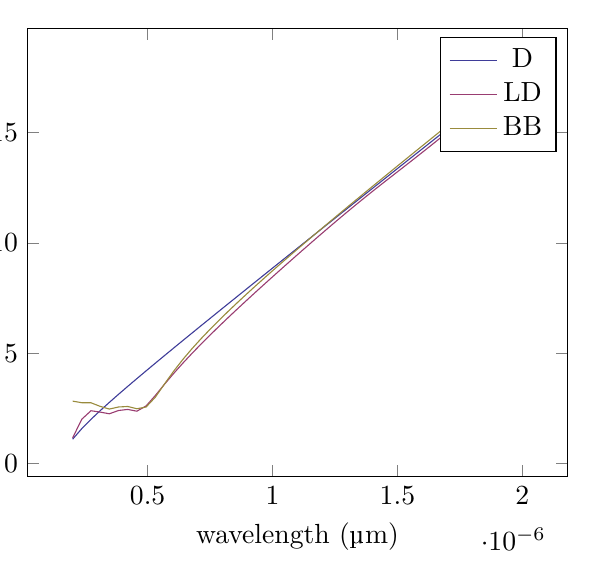
\begin{tikzpicture}[baseline,trim axis left]
			\begin{axis}[xlabel=wavelength (\si{\micro\meter}),ylabel=refractive index $n''$]
				\addplot[color=colora] coordinates {
						(2e-07, 1.1068167438804126)
						(2.3673469387755102e-07, 1.5869501259763072)
						(2.7346938775510205e-07, 2.0073109746535156)
						(3.1020408163265303e-07, 2.399512626854339)
						(3.4693877551020406e-07, 2.775510921004029)
						(3.836734693877551e-07, 3.1411229809127894)
						(4.2040816326530607e-07, 3.4995986483800734)
						(4.571428571428571e-07, 3.8529234736512987)
						(4.938775510204081e-07, 4.202389997207195)
						(5.306122448979591e-07, 4.548880679834958)
						(5.673469387755102e-07, 4.89302087876839)
						(6.040816326530612e-07, 5.235267263502626)
						(6.408163265306121e-07, 5.575961679028544)
						(6.775510204081632e-07, 5.915365392106543)
						(7.142857142857142e-07, 6.253681651385232)
						(7.510204081632653e-07, 6.5910710014750835)
						(7.877551020408163e-07, 6.927661949094492)
						(8.244897959183672e-07, 7.263558559683651)
						(8.612244897959183e-07, 7.598845974857824)
						(8.979591836734693e-07, 7.933594489840012)
						(9.346938775510204e-07, 8.267862613676728)
						(9.714285714285713e-07, 8.601699398137153)
						(1.0081632653061223e-06, 8.93514623245245)
						(1.0448979591836734e-06, 9.268238242275855)
						(1.0816326530612245e-06, 9.601005391554645)
						(1.1183673469387754e-06, 9.933473358729426)
						(1.1551020408163265e-06, 10.265664239630103)
						(1.1918367346938776e-06, 10.597597115942172)
						(1.2285714285714284e-06, 10.929288518425434)
						(1.2653061224489795e-06, 11.260752807020424)
						(1.3020408163265306e-06, 11.592002484795357)
						(1.3387755102040815e-06, 11.923048458834142)
						(1.3755102040816325e-06, 12.253900258274255)
						(1.4122448979591836e-06, 12.584566217512025)
						(1.4489795918367345e-06, 12.91505363091868)
						(1.4857142857142856e-06, 13.245368884120198)
						(1.5224489795918367e-06, 13.575517565892662)
						(1.5591836734693875e-06, 13.905504563941589)
						(1.5959183673469386e-06, 14.235334147217372)
						(1.6326530612244897e-06, 14.565010036930454)
						(1.6693877551020408e-06, 14.89453546804062)
						(1.7061224489795917e-06, 15.223913242682766)
						(1.7428571428571427e-06, 15.553145776739838)
						(1.7795918367346938e-06, 15.882235140569993)
						(1.8163265306122447e-06, 16.211183094728963)
						(1.8530612244897958e-06, 16.53999112139298)
						(1.8897959183673469e-06, 16.868660452075936)
						(1.9265306122448977e-06, 17.197192092142522)
						(1.963265306122449e-06, 17.525586842542825)
						(2e-06, 17.853845319130215)
					};
				\addlegendentry{D}
				\addplot[color=colorb] coordinates {
						(2e-07, 1.1681932338811492)
						(2.3673469387755102e-07, 2.014342789712326)
						(2.7346938775510205e-07, 2.396120606757039)
						(3.1020408163265303e-07, 2.334169100593518)
						(3.4693877551020406e-07, 2.2586076475155075)
						(3.836734693877551e-07, 2.4072946123184757)
						(4.2040816326530607e-07, 2.455686081165384)
						(4.571428571428571e-07, 2.3755360504962346)
						(4.938775510204081e-07, 2.6128689817393655)
						(5.306122448979591e-07, 3.082351255105427)
						(5.673469387755102e-07, 3.5920321715836323)
						(6.040816326530612e-07, 4.082926122930079)
						(6.408163265306121e-07, 4.548923237289287)
						(6.775510204081632e-07, 4.99389164811314)
						(7.142857142857142e-07, 5.42234044136973)
						(7.510204081632653e-07, 5.837906178826007)
						(7.877551020408163e-07, 6.243331455174237)
						(8.244897959183672e-07, 6.640667464759648)
						(8.612244897959183e-07, 7.031459911306562)
						(8.979591836734693e-07, 7.416885708949246)
						(9.346938775510204e-07, 7.7978473552990675)
						(9.714285714285713e-07, 8.175035941372315)
						(1.0081632653061223e-06, 8.54897124638577)
						(1.0448979591836734e-06, 8.920024440906737)
						(1.0816326530612245e-06, 9.28842677681269)
						(1.1183673469387754e-06, 9.654266499912424)
						(1.1551020408163265e-06, 10.017476360235198)
						(1.1918367346938776e-06, 10.37781615481617)
						(1.2285714285714284e-06, 10.734859700292114)
						(1.2653061224489795e-06, 11.088004181950721)
						(1.3020408163265306e-06, 11.436530311177645)
						(1.3387755102040815e-06, 11.779746286118186)
						(1.3755102040816325e-06, 12.11723025694682)
						(1.4122448979591836e-06, 12.449127263646576)
						(1.4489795918367345e-06, 12.776370143122527)
						(1.4857142857142856e-06, 13.100653898161305)
						(1.5224489795918367e-06, 13.424090615452474)
						(1.5591836734693875e-06, 13.748679330665253)
						(1.5959183673469386e-06, 14.075857847342018)
						(1.6326530612244897e-06, 14.406326257142965)
						(1.6693877551020408e-06, 14.740136776210091)
						(1.7061224489795917e-06, 15.076916802721703)
						(1.7428571428571427e-06, 15.41609360241849)
						(1.7795918367346938e-06, 15.757054904122587)
						(1.8163265306122447e-06, 16.099237548153443)
						(1.8530612244897958e-06, 16.44216273319327)
						(1.8897959183673469e-06, 16.785439963639618)
						(1.9265306122448977e-06, 17.128756197948686)
						(1.963265306122449e-06, 17.47186004776569)
						(2e-06, 17.814545990870027)
					};
				\addlegendentry{LD}
				\addplot[color=colorc] coordinates {
						(2e-07, 2.832198357410091)
						(2.3673469387755102e-07, 2.759813560824599)
						(2.7346938775510205e-07, 2.7563535023122445)
						(3.1020408163265303e-07, 2.5949116791202425)
						(3.4693877551020406e-07, 2.4717106477054247)
						(3.836734693877551e-07, 2.566853231558741)
						(4.2040816326530607e-07, 2.588982551315835)
						(4.571428571428571e-07, 2.4868090050490714)
						(4.938775510204081e-07, 2.5645306129181282)
						(5.306122448979591e-07, 3.0053243778762613)
						(5.673469387755102e-07, 3.604042124203765)
						(6.040816326530612e-07, 4.18530924459203)
						(6.408163265306121e-07, 4.717085059682472)
						(6.775510204081632e-07, 5.206624072132651)
						(7.142857142857142e-07, 5.664837442538714)
						(7.510204081632653e-07, 6.1001007722596565)
						(7.877551020408163e-07, 6.518181975776647)
						(8.244897959183672e-07, 6.923018023659372)
						(8.612244897959183e-07, 7.317358124118042)
						(8.979591836734693e-07, 7.703185221827967)
						(9.346938775510204e-07, 8.081977202852334)
						(9.714285714285713e-07, 8.454868420657379)
						(1.0081632653061223e-06, 8.822751555724386)
						(1.0448979591836734e-06, 9.186343712258719)
						(1.0816326530612245e-06, 9.546230684481692)
						(1.1183673469387754e-06, 9.902897550468035)
						(1.1551020408163265e-06, 10.256750455126637)
						(1.1918367346938776e-06, 10.608132548181485)
						(1.2285714285714284e-06, 10.957335933624886)
						(1.2653061224489795e-06, 11.304610823565145)
						(1.3020408163265306e-06, 11.65017268306313)
						(1.3387755102040815e-06, 11.994207897742331)
						(1.3755102040816325e-06, 12.336878332374608)
						(1.4122448979591836e-06, 12.678325041205843)
						(1.4489795918367345e-06, 13.018671318650483)
						(1.4857142857142856e-06, 13.35802522951232)
						(1.5224489795918367e-06, 13.696481723263922)
						(1.5591836734693875e-06, 14.03412441220898)
						(1.5959183673469386e-06, 14.371027075394238)
						(1.6326530612244897e-06, 14.707254936859977)
						(1.6693877551020408e-06, 15.042865756842724)
						(1.7061224489795917e-06, 15.377910766938319)
						(1.7428571428571427e-06, 15.712435474356345)
						(1.7795918367346938e-06, 16.046480355799982)
						(1.8163265306122447e-06, 16.380081457869824)
						(1.8530612244897958e-06, 16.7132709179868)
						(1.8897959183673469e-06, 17.046077417490107)
						(1.9265306122448977e-06, 17.37852657666669)
						(1.963265306122449e-06, 17.710641299915608)
						(2e-06, 18.042442077972584)
					};
				\addlegendentry{BB}
			\end{axis}
		\end{tikzpicture}%
		\\
	\end{tabular}
	\caption{Complex permittivity $\epsilon = \epsilon' + \mi \epsilon''$ and refractive index $n = n' + \mi n''$ for Au based on the Drude (D), Lorentz-Drude (LD), and Brendel-Bormann (BB) models.}
\end{figure}
\clearpage
\newpage
\subsection{Cu}
\begin{figure}[h!]
	\centering
	\begin{tabular}{l}
		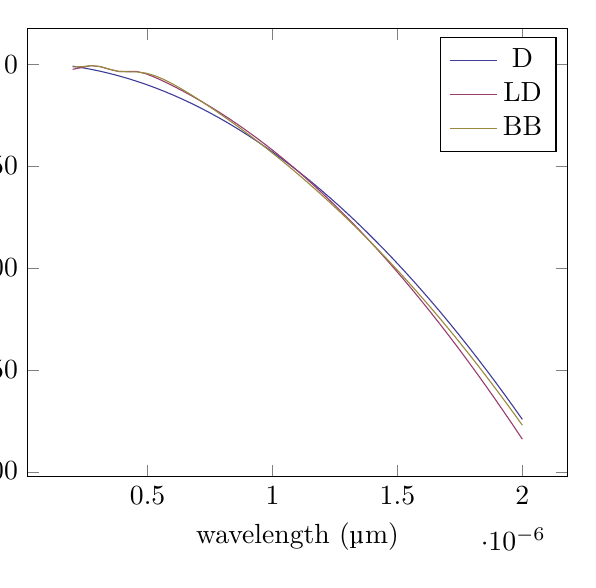
\begin{tikzpicture}[baseline,trim axis left]
			\begin{axis}[xlabel=wavelength (\si{\micro\meter}),ylabel=permittivity $\epsilon'$]
				\addplot[color=colora] coordinates {
						(2e-07, -0.754857682705983)
						(2.3673469387755102e-07, -1.458677966016431)
						(2.7346938775510205e-07, -2.280881178463082)
						(3.1020408163265303e-07, -3.221459525831647)
						(3.4693877551020406e-07, -4.280404092065389)
						(3.836734693877551e-07, -5.457704839476399)
						(4.2040816326530607e-07, -6.753350608983447)
						(4.571428571428571e-07, -8.167329120376376)
						(4.938775510204081e-07, -9.699626972607051)
						(5.306122448979591e-07, -11.350229644106825)
						(5.673469387755102e-07, -13.119121493130553)
						(6.040816326530612e-07, -15.00628575812705)
						(6.408163265306121e-07, -17.01170455813607)
						(6.775510204081632e-07, -19.135358893211784)
						(7.142857142857142e-07, -21.37722864487264)
						(7.510204081632653e-07, -23.73729257657767)
						(7.877551020408163e-07, -26.215528334229234)
						(8.244897959183672e-07, -28.811912446702145)
						(8.612244897959183e-07, -31.52642032639914)
						(8.979591836734693e-07, -34.35902626983264)
						(9.346938775510204e-07, -37.309703458232924)
						(9.714285714285713e-07, -40.3784239581825)
						(1.0081632653061223e-06, -43.56515872227685)
						(1.0448979591836734e-06, -46.869877589811175)
						(1.0816326530612245e-06, -50.292549287493635)
						(1.1183673469387754e-06, -53.83314143018444)
						(1.1551020408163265e-06, -57.49162052166145)
						(1.1918367346938776e-06, -61.26795195541146)
						(1.2285714285714284e-06, -65.16210001544782)
						(1.2653061224489795e-06, -69.17402787715406)
						(1.3020408163265306e-06, -73.30369760815343)
						(1.3387755102040815e-06, -77.55107016920435)
						(1.3755102040816325e-06, -81.91610541512203)
						(1.4122448979591836e-06, -86.39876209572557)
						(1.4489795918367345e-06, -90.99899785681122)
						(1.4857142857142856e-06, -95.71676924115125)
						(1.5224489795918367e-06, -100.5520316895188)
						(1.5591836734693875e-06, -105.50473954173796)
						(1.5959183673469386e-06, -110.57484603776004)
						(1.6326530612244897e-06, -115.76230331876515)
						(1.6693877551020408e-06, -121.06706242828918)
						(1.7061224489795917e-06, -126.4890733133769)
						(1.7428571428571427e-06, -132.02828482575987)
						(1.7795918367346938e-06, -137.68464472305993)
						(1.8163265306122447e-06, -143.45809967001833)
						(1.8530612244897958e-06, -149.34859523974984)
						(1.8897959183673469e-06, -155.3560759150222)
						(1.9265306122448977e-06, -161.48048508956072)
						(1.963265306122449e-06, -167.7217650693783)
						(2e-06, -174.07985707413005)
					};
				\addlegendentry{D}
				\addplot[color=colorb] coordinates {
						(2e-07, -2.2841480427359793)
						(2.3673469387755102e-07, -1.3934228186293052)
						(2.7346938775510205e-07, -0.44704457177167534)
						(3.1020408163265303e-07, -0.9600972004862669)
						(3.4693877551020406e-07, -2.2519207608982628)
						(3.836734693877551e-07, -3.3516577319948175)
						(4.2040816326530607e-07, -3.3460959887627864)
						(4.571428571428571e-07, -3.3547938819345324)
						(4.938775510204081e-07, -4.483028467438269)
						(5.306122448979591e-07, -6.27489908730486)
						(5.673469387755102e-07, -8.34789698737015)
						(6.040816326530612e-07, -10.573646963066864)
						(6.408163265306121e-07, -12.91755520291489)
						(6.775510204081632e-07, -15.372618144983484)
						(7.142857142857142e-07, -17.93943332461373)
						(7.510204081632653e-07, -20.6203473250144)
						(7.877551020408163e-07, -23.417766253080686)
						(8.244897959183672e-07, -26.333720114845544)
						(8.612244897959183e-07, -29.369805861358603)
						(8.979591836734693e-07, -32.52723604880905)
						(9.346938775510204e-07, -35.80690722982673)
						(9.714285714285713e-07, -39.20946258990308)
						(1.0081632653061223e-06, -42.73534302590544)
						(1.0448979591836734e-06, -46.38482700357496)
						(1.0816326530612245e-06, -50.15806111917075)
						(1.1183673469387754e-06, -54.05508339955671)
						(1.1551020408163265e-06, -58.07584106572452)
						(1.1918367346938776e-06, -62.22020411372305)
						(1.2285714285714284e-06, -66.48797574214501)
						(1.2653061224489795e-06, -70.8789003984668)
						(1.3020408163265306e-06, -75.39267002195294)
						(1.3387755102040815e-06, -80.02892891619692)
						(1.3755102040816325e-06, -84.78727757765314)
						(1.4122448979591836e-06, -89.66727572788045)
						(1.4489795918367345e-06, -94.66844473915496)
						(1.4857142857142856e-06, -99.79026960005581)
						(1.5224489795918367e-06, -105.03220053553258)
						(1.5591836734693875e-06, -110.39365437188822)
						(1.5959183673469386e-06, -115.87401571892904)
						(1.6326530612244897e-06, -121.47263802769524)
						(1.6693877551020408e-06, -127.18884457156682)
						(1.7061224489795917e-06, -133.0219293903125)
						(1.7428571428571427e-06, -138.97115823019763)
						(1.7795918367346938e-06, -145.03576950814687)
						(1.8163265306122447e-06, -151.21497532381542)
						(1.8530612244897958e-06, -157.5079625400143)
						(1.8897959183673469e-06, -163.913893949055)
						(1.9265306122448977e-06, -170.4319095400875)
						(1.963265306122449e-06, -177.06112788027943)
						(2e-06, -183.80064762064217)
					};
				\addlegendentry{LD}
				\addplot[color=colorc] coordinates {
						(2e-07, -1.0970571691085211)
						(2.3673469387755102e-07, -0.9466790347954035)
						(2.7346938775510205e-07, -0.4960950460808222)
						(3.1020408163265303e-07, -0.9078774038230311)
						(3.4693877551020406e-07, -2.2262238320577703)
						(3.836734693877551e-07, -3.271244296253267)
						(4.2040816326530607e-07, -3.4953781878675008)
						(4.571428571428571e-07, -3.5579420313938517)
						(4.938775510204081e-07, -4.156332360265321)
						(5.306122448979591e-07, -5.4772289174223125)
						(5.673469387755102e-07, -7.390946575076198)
						(6.040816326530612e-07, -9.707127578743414)
						(6.408163265306121e-07, -12.281493729982799)
						(6.775510204081632e-07, -15.027669279461865)
						(7.142857142857142e-07, -17.900045854746853)
						(7.510204081632653e-07, -20.87626407131636)
						(7.877551020408163e-07, -23.94579244552412)
						(8.244897959183672e-07, -27.103723179271974)
						(8.612244897959183e-07, -30.34775128795135)
						(8.979591836734693e-07, -33.67681784121103)
						(9.346938775510204e-07, -37.09053760376294)
						(9.714285714285713e-07, -40.58896366124825)
						(1.0081632653061223e-06, -44.17248210946251)
						(1.0448979591836734e-06, -47.841749935784286)
						(1.0816326530612245e-06, -51.59764426361508)
						(1.1183673469387754e-06, -55.44121411761314)
						(1.1551020408163265e-06, -59.37363418601594)
						(1.1918367346938776e-06, -63.396162212449795)
						(1.2285714285714284e-06, -67.51010154362392)
						(1.2653061224489795e-06, -71.71676964902699)
						(1.3020408163265306e-06, -76.0174727394952)
						(1.3387755102040815e-06, -80.41348612355455)
						(1.3755102040816325e-06, -84.90603966085189)
						(1.4122448979591836e-06, -89.49630755363225)
						(1.4489795918367345e-06, -94.1854017063323)
						(1.4857142857142856e-06, -98.97436793572531)
						(1.5224489795918367e-06, -103.86418439804619)
						(1.5591836734693875e-06, -108.8557616945617)
						(1.5959183673469386e-06, -113.94994421081574)
						(1.6326530612244897e-06, -119.14751233063994)
						(1.6693877551020408e-06, -124.44918524102646)
						(1.7061224489795917e-06, -129.85562410735997)
						(1.7428571428571427e-06, -135.36743545080628)
						(1.7795918367346938e-06, -140.98517460198033)
						(1.8163265306122447e-06, -146.70934913872006)
						(1.8530612244897958e-06, -152.5404222422678)
						(1.8897959183673469e-06, -158.4788159266839)
						(1.9265306122448977e-06, -164.52491411202863)
						(1.963265306122449e-06, -170.67906552371977)
						(2e-06, -176.94158640930547)
					};
				\addlegendentry{BB}
			\end{axis}
		\end{tikzpicture}%
		\\
		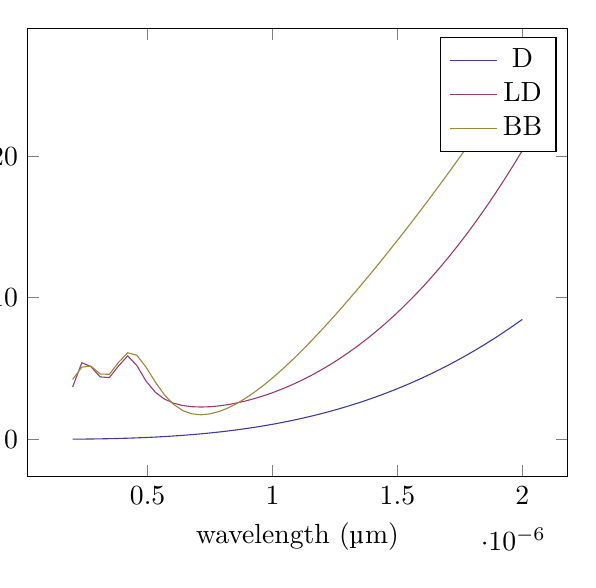
\begin{tikzpicture}[baseline,trim axis left]
			\begin{axis}[xlabel=wavelength (\si{\micro\meter}),ylabel=permittivity $\epsilon''$]
				\addplot[color=colora] coordinates {
						(2e-07, 0.008492329046195955)
						(2.3673469387755102e-07, 0.014083755421671174)
						(2.7346938775510205e-07, 0.021709715718046228)
						(3.1020408163265303e-07, 0.03168582751451724)
						(3.4693877551020406e-07, 0.044327671260961425)
						(3.836734693877551e-07, 0.059950785294117244)
						(4.2040816326530607e-07, 0.07887066085516178)
						(4.571428571428571e-07, 0.10140273710885016)
						(4.938775510204081e-07, 0.12786239616438214)
						(5.306122448979591e-07, 0.15856495809816146)
						(5.673469387755102e-07, 0.1938256759786118)
						(6.040816326530612e-07, 0.23395973089321484)
						(6.408163265306121e-07, 0.2792822269779346)
						(6.775510204081632e-07, 0.33010818644919354)
						(7.142857142857142e-07, 0.38675254463856346)
						(7.510204081632653e-07, 0.44953014503033567)
						(7.877551020408163e-07, 0.5187557343021351)
						(8.244897959183672e-07, 0.5947439573687431)
						(8.612244897959183e-07, 0.67780935242929)
						(8.979591836734693e-07, 0.7682663460179807)
						(9.346938775510204e-07, 0.866429248058523)
						(9.714285714285713e-07, 0.9726122469224112)
						(1.0081632653061223e-06, 1.08712940449124)
						(1.0448979591836734e-06, 1.2102946512231978)
						(1.0816326530612245e-06, 1.3424217812239154)
						(1.1183673469387754e-06, 1.4838244473218185)
						(1.1551020408163265e-06, 1.634816156148165)
						(1.1918367346938776e-06, 1.7957102632219017)
						(1.2285714285714284e-06, 1.9668199680395275)
						(1.2653061224489795e-06, 2.1484583091701124)
						(1.3020408163265306e-06, 2.340938159355632)
						(1.3387755102040815e-06, 2.544572220616777)
						(1.3755102040816325e-06, 2.7596730193644103)
						(1.4122448979591836e-06, 2.986552901516815)
						(1.4489795918367345e-06, 3.225524027622898)
						(1.4857142857142856e-06, 3.4768983679915237)
						(1.5224489795918367e-06, 3.740987697827108)
						(1.5591836734693875e-06, 4.018103592371654)
						(1.5959183673469386e-06, 4.30855742205338)
						(1.6326530612244897e-06, 4.612660347642103)
						(1.6693877551020408e-06, 4.930723315411503)
						(1.7061224489795917e-06, 5.263057052308507)
						(1.7428571428571427e-06, 5.609972061129829)
						(1.7795918367346938e-06, 5.971778615705932)
						(1.8163265306122447e-06, 6.348786756092502)
						(1.8530612244897958e-06, 6.741306283769636)
						(1.8897959183673469e-06, 7.14964675684883)
						(1.9265306122448977e-06, 7.5741174852879904)
						(1.963265306122449e-06, 8.01502752611463)
						(2e-06, 8.472685678657298)
					};
				\addlegendentry{D}
				\addplot[color=colorb] coordinates {
						(2e-07, 3.7032699526622768)
						(2.3673469387755102e-07, 5.410501017582086)
						(2.7346938775510205e-07, 5.132259000208603)
						(3.1020408163265303e-07, 4.408055589796272)
						(3.4693877551020406e-07, 4.3613358493574585)
						(3.836734693877551e-07, 5.18329464234179)
						(4.2040816326530607e-07, 5.894797741946914)
						(4.571428571428571e-07, 5.209722899172)
						(4.938775510204081e-07, 4.113137889542716)
						(5.306122448979591e-07, 3.3275185227786124)
						(5.673469387755102e-07, 2.8429415923346313)
						(6.040816326530612e-07, 2.5528728777845227)
						(6.408163265306121e-07, 2.38636489006107)
						(6.775510204081632e-07, 2.302991036182498)
						(7.142857142857142e-07, 2.2796844688613005)
						(7.510204081632653e-07, 2.3028575241516447)
						(7.877551020408163e-07, 2.364236233740703)
						(8.244897959183672e-07, 2.4586507392615786)
						(8.612244897959183e-07, 2.5828227891774933)
						(8.979591836734693e-07, 2.7346728519168275)
						(9.346938775510204e-07, 2.91290803948728)
						(9.714285714285713e-07, 3.1167677869679453)
						(1.0081632653061223e-06, 3.3458615176390327)
						(1.0448979591836734e-06, 3.6000618168625302)
						(1.0816326530612245e-06, 3.879432161521736)
						(1.1183673469387754e-06, 4.184176771713579)
						(1.1551020408163265e-06, 4.51460498444912)
						(1.1918367346938776e-06, 4.871105376015249)
						(1.2285714285714284e-06, 5.254126560352793)
						(1.2653061224489795e-06, 5.664162640741538)
						(1.3020408163265306e-06, 6.101741955800353)
						(1.3387755102040815e-06, 6.567418189611535)
						(1.3755102040816325e-06, 7.061763198423723)
						(1.4122448979591836e-06, 7.585361096188569)
						(1.4489795918367345e-06, 8.138803270867934)
						(1.4857142857142856e-06, 8.722684093507237)
						(1.5224489795918367e-06, 9.337597145586905)
						(1.5591836734693875e-06, 9.984131835630574)
						(1.5959183673469386e-06, 10.662870309069312)
						(1.6326530612244897e-06, 11.374384579688858)
						(1.6693877551020408e-06, 12.119233829170016)
						(1.7061224489795917e-06, 12.897961835023455)
						(1.7428571428571427e-06, 13.71109449783826)
						(1.7795918367346938e-06, 14.559137447066405)
						(1.8163265306122447e-06, 15.442573711159984)
						(1.8530612244897958e-06, 16.361861443200105)
						(1.8897959183673469e-06, 17.317431697516923)
						(1.9265306122448977e-06, 18.309686256426218)
						(1.963265306122449e-06, 19.338995509259863)
						(2e-06, 20.405696388463067)
					};
				\addlegendentry{LD}
				\addplot[color=colorc] coordinates {
						(2e-07, 4.230870917943947)
						(2.3673469387755102e-07, 5.09830236643376)
						(2.7346938775510205e-07, 5.170327464134542)
						(3.1020408163265303e-07, 4.612077672507162)
						(3.4693877551020406e-07, 4.592014233255544)
						(3.836734693877551e-07, 5.432942866124943)
						(4.2040816326530607e-07, 6.115333952795469)
						(4.571428571428571e-07, 5.937229517024417)
						(4.938775510204081e-07, 5.093677777315964)
						(5.306122448979591e-07, 4.056811413786518)
						(5.673469387755102e-07, 3.1415311399523294)
						(6.040816326530612e-07, 2.463763739448778)
						(6.408163265306121e-07, 2.027615421915652)
						(6.775510204081632e-07, 1.79740558139142)
						(7.142857142857142e-07, 1.7326251877642584)
						(7.510204081632653e-07, 1.7995632670444832)
						(7.877551020408163e-07, 1.9728370060081108)
						(8.244897959183672e-07, 2.2337867878970767)
						(8.612244897959183e-07, 2.5684972330000315)
						(8.979591836734693e-07, 2.9662497832951633)
						(9.346938775510204e-07, 3.418486308599724)
						(9.714285714285713e-07, 3.9181627821815104)
						(1.0081632653061223e-06, 4.459357180369349)
						(1.0448979591836734e-06, 5.037029617444837)
						(1.0816326530612245e-06, 5.646868914062635)
						(1.1183673469387754e-06, 6.2851866523128335)
						(1.1551020408163265e-06, 6.948837064430537)
						(1.1918367346938776e-06, 7.635151361776558)
						(1.2285714285714284e-06, 8.341880834799671)
						(1.2653061224489795e-06, 9.067146069012095)
						(1.3020408163265306e-06, 9.809391106211221)
						(1.3387755102040815e-06, 10.567342044527717)
						(1.3755102040816325e-06, 11.339969821767912)
						(1.4122448979591836e-06, 12.126456986098562)
						(1.4489795918367345e-06, 12.926168241867387)
						(1.4857142857142856e-06, 13.738624522369818)
						(1.5224489795918367e-06, 14.563480310060651)
						(1.5591836734693875e-06, 15.400503906389682)
						(1.5959183673469386e-06, 16.24956034888306)
						(1.6326530612244897e-06, 17.110596679990813)
						(1.6693877551020408e-06, 17.983629287415393)
						(1.7061224489795917e-06, 18.86873305611772)
						(1.7428571428571427e-06, 19.76603209549532)
						(1.7795918367346938e-06, 20.675691829483306)
						(1.8163265306122447e-06, 21.597912261243746)
						(1.8530612244897958e-06, 22.532922246835938)
						(1.8897959183673469e-06, 23.480974633300402)
						(1.9265306122448977e-06, 24.44234213569328)
						(1.963265306122449e-06, 25.41731384470205)
						(2e-06, 26.406192271592495)
					};
				\addlegendentry{BB}
			\end{axis}
		\end{tikzpicture}%
		\\
		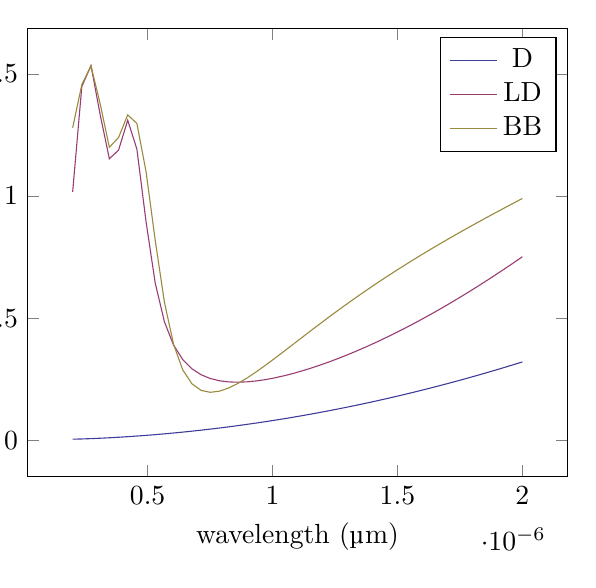
\begin{tikzpicture}[baseline,trim axis left]
			\begin{axis}[xlabel=wavelength (\si{\micro\meter}),ylabel=refractive index $n'$]
				\addplot[color=colora] coordinates {
						(2e-07, 0.004887169559408782)
						(2.3673469387755102e-07, 0.005830471904026147)
						(2.7346938775510205e-07, 0.007187335074675955)
						(3.1020408163265303e-07, 0.008826803665840682)
						(3.4693877551020406e-07, 0.010712645007780087)
						(3.836734693877551e-07, 0.012830787377628805)
						(4.2040816326530607e-07, 0.015174641214544838)
						(4.571428571428571e-07, 0.017740721818063576)
						(4.938775510204081e-07, 0.020527019466910313)
						(5.306122448979591e-07, 0.023532296027563043)
						(5.673469387755102e-07, 0.026755747322510223)
						(6.040816326530612e-07, 0.03019682742057901)
						(6.408163265306121e-07, 0.03385515117615388)
						(6.775510204081632e-07, 0.03773043730248556)
						(7.142857142857142e-07, 0.04182247366532046)
						(7.510204081632653e-07, 0.046131095344350545)
						(7.877551020408163e-07, 0.05065617032975707)
						(8.244897959183672e-07, 0.05539758994289019)
						(8.612244897959183e-07, 0.060355262268336284)
						(8.979591836734693e-07, 0.06552910755647985)
						(9.346938775510204e-07, 0.07091905494504315)
						(9.714285714285713e-07, 0.07652504008222019)
						(1.0081632653061223e-06, 0.08234700337775556)
						(1.0448979591836734e-06, 0.08838488869812218)
						(1.0816326530612245e-06, 0.0946386423811374)
						(1.1183673469387754e-06, 0.10110821248346352)
						(1.1551020408163265e-06, 0.10779354819980327)
						(1.1918367346938776e-06, 0.11469459941030608)
						(1.2285714285714284e-06, 0.1218113163249622)
						(1.2653061224489795e-06, 0.12914364920164817)
						(1.3020408163265306e-06, 0.13669154812114073)
						(1.3387755102040815e-06, 0.14445496280608738)
						(1.3755102040816325e-06, 0.15243384247450653)
						(1.4122448979591836e-06, 0.16062813572067197)
						(1.4489795918367345e-06, 0.16903779041725583)
						(1.4857142857142856e-06, 0.17766275363511283)
						(1.5224489795918367e-06, 0.18650297157666512)
						(1.5591836734693875e-06, 0.19555838952083518)
						(1.5959183673469386e-06, 0.2048289517767923)
						(1.6326530612244897e-06, 0.21431460164548208)
						(1.6693877551020408e-06, 0.2240152813871863)
						(1.7061224489795917e-06, 0.2339309321941804)
						(1.7428571428571427e-06, 0.2440614941677147)
						(1.7795918367346938e-06, 0.25440690629841184)
						(1.8163265306122447e-06, 0.26496710644968485)
						(1.8530612244897958e-06, 0.2757420313436365)
						(1.8897959183673469e-06, 0.2867316165491618)
						(1.9265306122448977e-06, 0.29793579647156954)
						(1.963265306122449e-06, 0.3093545043440346)
						(2e-06, 0.3209876722201777)
					};
				\addlegendentry{D}
				\addplot[color=colorb] coordinates {
						(2e-07, 1.0165852116995329)
						(2.3673469387755102e-07, 1.4480381615800753)
						(2.7346938775510205e-07, 1.533728709539404)
						(3.1020408163265303e-07, 1.3325359266692172)
						(3.4693877551020406e-07, 1.15249293847869)
						(3.836734693877551e-07, 1.187618288525839)
						(4.2040816326530607e-07, 1.3099958088083792)
						(4.571428571428571e-07, 1.1919825897663525)
						(4.938775510204081e-07, 0.8947076925389256)
						(5.306122448979591e-07, 0.6433069368083548)
						(5.673469387755102e-07, 0.4851886890091357)
						(6.040816326530612e-07, 0.3897528696438675)
						(6.408163265306121e-07, 0.33058812832487555)
						(6.775510204081632e-07, 0.2928735013870804)
						(7.142857142857142e-07, 0.2685771097769384)
						(7.510204081632653e-07, 0.2531716989305913)
						(7.877551020408163e-07, 0.24397027281925354)
						(8.244897959183672e-07, 0.23929799261977094)
						(8.612244897959183e-07, 0.23806494526776856)
						(8.979591836734693e-07, 0.23953506581711498)
						(9.346938775510204e-07, 0.24319519883809632)
						(9.714285714285713e-07, 0.24867767277030473)
						(1.0081632653061223e-06, 0.25571274118405896)
						(1.0448979591836734e-06, 0.2640983677616015)
						(1.0816326530612245e-06, 0.273680448044029)
						(1.1183673469387754e-06, 0.2843395148604756)
						(1.1551020408163265e-06, 0.29598158795275675)
						(1.1918367346938776e-06, 0.3085317408490872)
						(1.2285714285714284e-06, 0.3219294906337128)
						(1.2653061224489795e-06, 0.33612543612221063)
						(1.3020408163265306e-06, 0.3510787671129919)
						(1.3387755102040815e-06, 0.366755391822552)
						(1.3755102040816325e-06, 0.38312650986332997)
						(1.4122448979591836e-06, 0.40016751091104363)
						(1.4489795918367345e-06, 0.41785711456619573)
						(1.4857142857142856e-06, 0.4361766909958469)
						(1.5224489795918367e-06, 0.4551097185983096)
						(1.5591836734693875e-06, 0.4746413466193004)
						(1.5959183673469386e-06, 0.4947580389565752)
						(1.6326530612244897e-06, 0.515447281370754)
						(1.6693877551020408e-06, 0.5366973386752022)
						(1.7061224489795917e-06, 0.5584970516835007)
						(1.7428571428571427e-06, 0.5808356660775083)
						(1.7795918367346938e-06, 0.6037026871489286)
						(1.8163265306122447e-06, 0.6270877557239432)
						(1.8530612244897958e-06, 0.650980541616402)
						(1.8897959183673469e-06, 0.6753706517538974)
						(1.9265306122448977e-06, 0.7002475507398579)
						(1.963265306122449e-06, 0.7256004920988262)
						(2e-06, 0.7514184588319709)
					};
				\addlegendentry{LD}
				\addplot[color=colorc] coordinates {
						(2e-07, 1.279400757069054)
						(2.3673469387755102e-07, 1.4558108786651185)
						(2.7346938775510205e-07, 1.5326412090624544)
						(3.1020408163265303e-07, 1.377081671799203)
						(3.4693877551020406e-07, 1.199370217320229)
						(3.836734693877551e-07, 1.239055027219413)
						(4.2040816326530607e-07, 1.3319932141784574)
						(4.571428571428571e-07, 1.296868801631271)
						(4.938775510204081e-07, 1.099524713693161)
						(5.306122448979591e-07, 0.8181575970876614)
						(5.673469387755102e-07, 0.5656635855144341)
						(6.040816326530612e-07, 0.3922908251004459)
						(6.408163265306121e-07, 0.2883136668107545)
						(6.775510204081632e-07, 0.23141835324471333)
						(7.142857142857142e-07, 0.20452232059739797)
						(7.510204081632653e-07, 0.19674715656607714)
						(7.877551020408163e-07, 0.20140908377241068)
						(8.244897959183672e-07, 0.21435293862797883)
						(8.612244897959183e-07, 0.23291530290003537)
						(8.979591836734693e-07, 0.2553243643728722)
						(9.346938775510204e-07, 0.2803577745856178)
						(9.714285714285713e-07, 0.3071456588649082)
						(1.0081632653061223e-06, 0.3350543007782562)
						(1.0448979591836734e-06, 0.363614922844736)
						(1.0816326530612245e-06, 0.39247813763840156)
						(1.1183673469387754e-06, 0.42138343787960275)
						(1.1551020408163265e-06, 0.45013783841890537)
						(1.1918367346938776e-06, 0.4786003426308763)
						(1.2285714285714284e-06, 0.5066702962866437)
						(1.2653061224489795e-06, 0.5342784576478352)
						(1.3020408163265306e-06, 0.5613800429305562)
						(1.3387755102040815e-06, 0.5879492553085888)
						(1.3755102040816325e-06, 0.6139749551855993)
						(1.4122448979591836e-06, 0.6394572233967376)
						(1.4489795918367345e-06, 0.6644046309471401)
						(1.4857142857142856e-06, 0.6888320717769549)
						(1.5224489795918367e-06, 0.7127590460467699)
						(1.5591836734693875e-06, 0.7362083046685823)
						(1.5959183673469386e-06, 0.7592047836913378)
						(1.6326530612244897e-06, 0.7817747711842071)
						(1.6693877551020408e-06, 0.8039452604166104)
						(1.7061224489795917e-06, 0.8257434520750301)
						(1.7428571428571427e-06, 0.8471963754580963)
						(1.7795918367346938e-06, 0.8683306044082344)
						(1.8163265306122447e-06, 0.8891720484427115)
						(1.8530612244897958e-06, 0.9097458033539144)
						(1.8897959183673469e-06, 0.9300760486292337)
						(1.9265306122448977e-06, 0.9501859815323299)
						(1.963265306122449e-06, 0.9700977797017587)
						(2e-06, 0.9898325857497318)
					};
				\addlegendentry{BB}
			\end{axis}
		\end{tikzpicture}%
		\\
		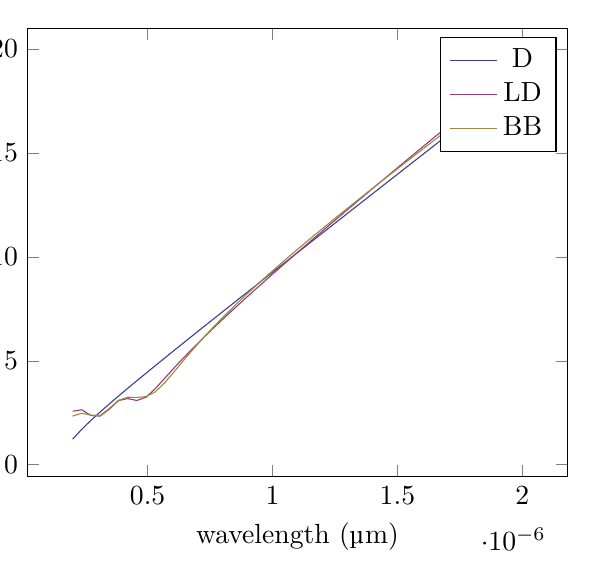
\begin{tikzpicture}[baseline,trim axis left]
			\begin{axis}[xlabel=wavelength (\si{\micro\meter}),ylabel=refractive index $n''$]
				\addplot[color=colora] coordinates {
						(2e-07, 1.2287241896636407)
						(2.3673469387755102e-07, 1.7080468145920678)
						(2.7346938775510205e-07, 2.1358524463307655)
						(3.1020408163265303e-07, 2.5383212713502608)
						(3.4693877551020406e-07, 2.925925102537128)
						(3.836734693877551e-07, 3.3038975373280355)
						(4.2040816326530607e-07, 3.675209076697389)
						(4.571428571428571e-07, 4.041693668151262)
						(4.938775510204081e-07, 4.404554082114385)
						(5.306122448979591e-07, 4.764616125788762)
						(5.673469387755102e-07, 5.122467640336119)
						(6.040816326530612e-07, 5.478539514599364)
						(6.408163265306121e-07, 5.833155360419818)
						(6.775510204081632e-07, 6.186563259049538)
						(7.142857142857142e-07, 6.538956761468319)
						(7.510204081632653e-07, 6.89048919229039)
						(7.877551020408163e-07, 7.2412836406015355)
						(8.244897959183672e-07, 7.591440092587654)
						(8.612244897959183e-07, 7.9410406224981145)
						(8.979591836734693e-07, 8.290153235467942)
						(9.346938775510204e-07, 8.638834755982687)
						(9.714285714285713e-07, 8.987133028941107)
						(1.0081632653061223e-06, 9.335088617816345)
						(1.0448979591836734e-06, 9.682736129665143)
						(1.0816326530612245e-06, 10.03010525967952)
						(1.1183673469387754e-06, 10.377221622459071)
						(1.1551020408163265e-06, 10.724107419332851)
						(1.1918367346938776e-06, 11.070781978392073)
						(1.2285714285714284e-06, 11.417262194784934)
						(1.2653061224489795e-06, 11.763562892192414)
						(1.3020408163265306e-06, 12.10969712152052)
						(1.3387755102040815e-06, 12.455676409210675)
						(1.3755102040816325e-06, 12.801510964839547)
						(1.4122448979591836e-06, 13.14720985560896)
						(1.4489795918367345e-06, 13.492781153742943)
						(1.4857142857142856e-06, 13.83823206158796)
						(1.5224489795918367e-06, 14.183569018263755)
						(1.5591836734693875e-06, 14.528797790970177)
						(1.5959183673469386e-06, 14.873923553470753)
						(1.6326530612244897e-06, 15.218950953810424)
						(1.6693877551020408e-06, 15.563884172955294)
						(1.7061224489795917e-06, 15.908726975745994)
						(1.7428571428571427e-06, 16.253482755317105)
						(1.7795918367346938e-06, 16.59815457194156)
						(1.8163265306122447e-06, 16.942745187101096)
						(1.8530612244897958e-06, 17.287257093454667)
						(1.8897959183673469e-06, 17.631692541270738)
						(1.9265306122448977e-06, 17.976053561801592)
						(1.963265306122449e-06, 18.320341988005367)
						(2e-06, 18.664559472960907)
					};
				\addlegendentry{D}
				\addplot[color=colorb] coordinates {
						(2e-07, 2.5758856866647495)
						(2.3673469387755102e-07, 2.6420587942063323)
						(2.7346938775510205e-07, 2.3661649672992295)
						(3.1020408163265303e-07, 2.339123423999023)
						(3.4693877551020406e-07, 2.6758777005466854)
						(3.836734693877551e-07, 3.0861286205328065)
						(4.2040816326530607e-07, 3.181881521319833)
						(4.571428571428571e-07, 3.0905068763038313)
						(4.938775510204081e-07, 3.2507015619790747)
						(5.306122448979591e-07, 3.65752454598752)
						(5.673469387755102e-07, 4.14326080552807)
						(6.040816326530612e-07, 4.631534143771908)
						(6.408163265306121e-07, 5.104281284079911)
						(6.775510204081632e-07, 5.560286509308349)
						(7.142857142857142e-07, 6.001927521806618)
						(7.510204081632653e-07, 6.431864929264886)
						(7.877551020408163e-07, 6.852340876970466)
						(8.244897959183672e-07, 7.265119908730674)
						(8.612244897959183e-07, 7.671568389778448)
						(8.979591836734693e-07, 8.07274588929505)
						(9.346938775510204e-07, 8.469480637508374)
						(9.714285714285713e-07, 8.862426662583735)
						(1.0081632653061223e-06, 9.252105925886204)
						(1.0448979591836734e-06, 9.638939251953952)
						(1.0816326530612245e-06, 10.023269138041973)
						(1.1183673469387754e-06, 10.405376721605787)
						(1.1551020408163265e-06, 10.785494533504854)
						(1.1918367346938776e-06, 11.16381618881594)
						(1.2285714285714284e-06, 11.540503831209856)
						(1.2653061224489795e-06, 11.915693912422821)
						(1.3020408163265306e-06, 12.289501724860166)
						(1.3387755102040815e-06, 12.662024990784676)
						(1.3755102040816325e-06, 13.033346730614758)
						(1.4122448979591836e-06, 13.403537575182844)
						(1.4489795918367345e-06, 13.772657645302054)
						(1.4857142857142856e-06, 14.140758091829722)
						(1.5224489795918367e-06, 14.507882367285394)
						(1.5591836734693875e-06, 14.87406728368598)
						(1.5959183673469386e-06, 15.23934389900308)
						(1.6326530612244897e-06, 15.603738265400874)
						(1.6693877551020408e-06, 15.967272065378472)
						(1.7061224489795917e-06, 16.329963156544576)
						(1.7428571428571427e-06, 16.69182604158007)
						(1.7795918367346938e-06, 17.0528722766939)
						(1.8163265306122447e-06, 17.413110829325948)
						(1.8530612244897958e-06, 17.772548393833535)
						(1.8897959183673469e-06, 18.131189672291526)
						(1.9265306122448977e-06, 18.489037626247868)
						(1.963265306122449e-06, 18.846093704235553)
						(2e-06, 19.202358048995734)
					};
				\addlegendentry{LD}
				\addplot[color=colorc] coordinates {
						(2e-07, 2.3383427748289556)
						(2.3673469387755102e-07, 2.4763135299210832)
						(2.7346938775510205e-07, 2.3854073538065754)
						(3.1020408163265303e-07, 2.3682193034549477)
						(3.4693877551020406e-07, 2.707291173942154)
						(3.836734693877551e-07, 3.100484367556452)
						(4.2040816326530607e-07, 3.24640851110422)
						(4.571428571428571e-07, 3.2372243419443087)
						(4.938775510204081e-07, 3.275755472036137)
						(5.306122448979591e-07, 3.5061690692533833)
						(5.673469387755102e-07, 3.927065537281812)
						(6.040816326530612e-07, 4.440950274479867)
						(6.408163265306121e-07, 4.972849987774146)
						(6.775510204081632e-07, 5.492034911338485)
						(7.142857142857142e-07, 5.990304705834153)
						(7.510204081632653e-07, 6.467607519776257)
						(7.877551020408163e-07, 6.926233906611898)
						(8.244897959183672e-07, 7.368808636621041)
						(8.612244897959183e-07, 7.797692072180892)
						(8.979591836734693e-07, 8.214865595036043)
						(9.346938775510204e-07, 8.621964751207644)
						(9.714285714285713e-07, 9.020343908854896)
						(1.0081632653061223e-06, 9.411136328194647)
						(1.0448979591836734e-06, 9.795301501015645)
						(1.0816326530612245e-06, 10.173660437830543)
						(1.1183673469387754e-06, 10.546921647507615)
						(1.1551020408163265e-06, 10.915700459392644)
						(1.1918367346938776e-06, 11.280533719679774)
						(1.2285714285714284e-06, 11.641891283873347)
						(1.2653061224489795e-06, 12.000185258514431)
						(1.3020408163265306e-06, 12.355777619566963)
						(1.3387755102040815e-06, 12.708986619740573)
						(1.3755102040816325e-06, 13.060092258973292)
						(1.4122448979591836e-06, 13.409341004999948)
						(1.4489795918367345e-06, 13.7569498959585)
						(1.4857142857142856e-06, 14.103110122156307)
						(1.5224489795918367e-06, 14.44799016166385)
						(1.5591836734693875e-06, 14.791738529491704)
						(1.5959183673469386e-06, 15.13448618978494)
						(1.6326530612244897e-06, 15.476348672959011)
						(1.6693877551020408e-06, 15.817427933945062)
						(1.7061224489795917e-06, 16.157813983086)
						(1.7428571428571427e-06, 16.497586317361435)
						(1.7795918367346938e-06, 16.836815176305304)
						(1.8163265306122447e-06, 17.175562644085453)
						(1.8530612244897958e-06, 17.513883616661833)
						(1.8897959183673469e-06, 17.851826650677385)
						(1.9265306122448977e-06, 18.189434708727436)
						(1.963265306122449e-06, 18.52674581387147)
						(2e-06, 18.863793624672503)
					};
				\addlegendentry{BB}
			\end{axis}
		\end{tikzpicture}%
		\\
	\end{tabular}
	\caption{Complex permittivity $\epsilon = \epsilon' + \mi \epsilon''$ and refractive index $n = n' + \mi n''$ for Cu based on the Drude (D), Lorentz-Drude (LD), and Brendel-Bormann (BB) models.}
\end{figure}
\clearpage
\newpage
\subsection{Cr}
\begin{figure}[h!]
	\centering
	\begin{tabular}{l}
		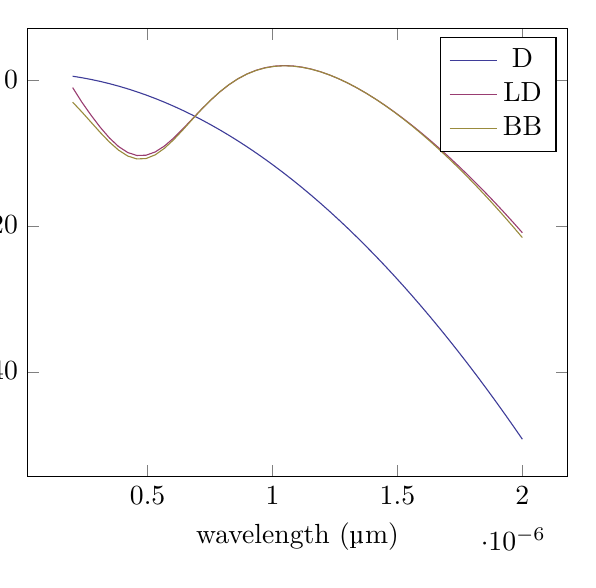
\begin{tikzpicture}[baseline,trim axis left]
			\begin{axis}[xlabel=wavelength (\si{\micro\meter}),ylabel=permittivity $\epsilon'$]
				\addplot[color=colora] coordinates {
						(2e-07, 0.4948404573143149)
						(2.3673469387755102e-07, 0.29224592803007465)
						(2.7346938775510205e-07, 0.05558190562390963)
						(3.1020408163265303e-07, -0.21514610430233705)
						(3.4693877551020406e-07, -0.5199318042492693)
						(3.836734693877551e-07, -0.8587681051860931)
						(4.2040816326530607e-07, -1.2316471269627391)
						(4.571428571428571e-07, -1.6385601987679048)
						(4.938775510204081e-07, -2.0794978596329607)
						(5.306122448979591e-07, -2.5544498589816795)
						(5.673469387755102e-07, -3.0634051572257155)
						(6.040816326530612e-07, -3.606351926405771)
						(6.408163265306121e-07, -4.18327755087839)
						(6.775510204081632e-07, -4.794168628048302)
						(7.142857142857142e-07, -5.43901096914622)
						(7.510204081632653e-07, -6.117789600052033)
						(7.877551020408163e-07, -6.830488762163285)
						(8.244897959183672e-07, -7.577091913308871)
						(8.612244897959183e-07, -8.357581728707812)
						(8.979591836734693e-07, -9.17194010197303)
						(9.346938775510204e-07, -10.020148146160043)
						(9.714285714285713e-07, -10.902186194860377)
						(1.0081632653061223e-06, -11.818033803339723)
						(1.0448979591836734e-06, -12.767669749720529)
						(1.0816326530612245e-06, -13.75107203620909)
						(1.1183673469387754e-06, -14.768217890366824)
						(1.1551020408163265e-06, -15.819083766425813)
						(1.1918367346938776e-06, -16.90364534664818)
						(1.2285714285714284e-06, -18.021877542729463)
						(1.2653061224489795e-06, -19.173754497245596)
						(1.3020408163265306e-06, -20.3592495851435)
						(1.3387755102040815e-06, -21.57833541527497)
						(1.3755102040816325e-06, -22.83098383197392)
						(1.4122448979591836e-06, -24.117165916676527)
						(1.4489795918367345e-06, -25.436851989584333)
						(1.4857142857142856e-06, -26.79001161137011)
						(1.5224489795918367e-06, -28.17661358492609)
						(1.5591836734693875e-06, -29.596625957154647)
						(1.5959183673469386e-06, -31.05001602080108)
						(1.6326530612244897e-06, -32.536750316328344)
						(1.6693877551020408e-06, -34.05679463383348)
						(1.7061224489795917e-06, -35.61011401500573)
						(1.7428571428571427e-06, -37.196672755125775)
						(1.7795918367346938e-06, -38.8164344051063)
						(1.8163265306122447e-06, -40.46936177357327)
						(1.8530612244897958e-06, -42.1554169289881)
						(1.8897959183673469e-06, -43.8745612018101)
						(1.9265306122448977e-06, -45.62675518669921)
						(1.963265306122449e-06, -47.4119587447588)
						(2e-06, -49.23013100581815)
					};
				\addlegendentry{D}
				\addplot[color=colorb] coordinates {
						(2e-07, -1.0600873812671048)
						(2.3673469387755102e-07, -3.051901968872664)
						(2.7346938775510205e-07, -4.839439850013817)
						(3.1020408163265303e-07, -6.490671222249466)
						(3.4693877551020406e-07, -7.950427678945559)
						(3.836734693877551e-07, -9.13323408483592)
						(4.2040816326530607e-07, -9.956563541753928)
						(4.571428571428571e-07, -10.361703376993622)
						(4.938775510204081e-07, -10.327553537346613)
						(5.306122448979591e-07, -9.87582596181)
						(5.673469387755102e-07, -9.066742134147507)
						(6.040816326530612e-07, -7.98714598704919)
						(6.408163265306121e-07, -6.735226434281427)
						(6.775510204081632e-07, -5.40634423878543)
						(7.142857142857142e-07, -4.08295924618483)
						(7.510204081632653e-07, -2.8295382959234496)
						(7.877551020408163e-07, -1.6916955663215436)
						(8.244897959183672e-07, -0.6980984698255792)
						(8.612244897959183e-07, 0.1363038552061102)
						(8.979591836734693e-07, 0.8067834284732509)
						(9.346938775510204e-07, 1.3156749872098672)
						(9.714285714285713e-07, 1.6698131234193223)
						(1.0081632653061223e-06, 1.8786029801979094)
						(1.0448979591836734e-06, 1.952652145132932)
						(1.0816326530612245e-06, 1.9028519059748898)
						(1.1183673469387754e-06, 1.739795141797977)
						(1.1551020408163265e-06, 1.4734342083650418)
						(1.1918367346938776e-06, 1.1129029924295075)
						(1.2285714285714284e-06, 0.6664469492482503)
						(1.2653061224489795e-06, 0.14142116971736485)
						(1.3020408163265306e-06, -0.45567101953966826)
						(1.3387755102040815e-06, -1.1191173068833429)
						(1.3755102040816325e-06, -1.843925437068929)
						(1.4122448979591836e-06, -2.6257495448613)
						(1.4489795918367345e-06, -3.4608182925915827)
						(1.4857142857142856e-06, -4.345867351271821)
						(1.5224489795918367e-06, -5.278077492648816)
						(1.5591836734693875e-06, -6.2550187603516285)
						(1.5959183673469386e-06, -7.2746007037278595)
						(1.6326530612244897e-06, -8.33502837944129)
						(1.6693877551020408e-06, -9.434763679916014)
						(1.7061224489795917e-06, -10.57249148512901)
						(1.7428571428571427e-06, -11.74709012261264)
						(1.7795918367346938e-06, -12.957605638653611)
						(1.8163265306122447e-06, -14.203229417945728)
						(1.8530612244897958e-06, -15.483278730777002)
						(1.8897959183673469e-06, -16.797179830920378)
						(1.9265306122448977e-06, -18.144453270620744)
						(1.963265306122449e-06, -19.524701139685824)
						(2e-06, -20.93759597283001)
					};
				\addlegendentry{LD}
				\addplot[color=colorc] coordinates {
						(2e-07, -3.0582826034650727)
						(2.3673469387755102e-07, -4.393158962091477)
						(2.7346938775510205e-07, -5.796688060965806)
						(3.1020408163265303e-07, -7.199321715725548)
						(3.4693877551020406e-07, -8.51241486254763)
						(3.836734693877551e-07, -9.629215565139209)
						(4.2040816326530607e-07, -10.43650543443373)
						(4.571428571428571e-07, -10.837868981498568)
						(4.938775510204081e-07, -10.780816298030786)
						(5.306122448979591e-07, -10.273533111417512)
						(5.673469387755102e-07, -9.381752008166087)
						(6.040816326530612e-07, -8.208802592289777)
						(6.408163265306121e-07, -6.870190999744665)
						(6.775510204081632e-07, -5.472920672972912)
						(7.142857142857142e-07, -4.103780805421196)
						(7.510204081632653e-07, -2.8257920318031795)
						(7.877551020408163e-07, -1.6799122330025487)
						(8.244897959183672e-07, -0.6891781624467326)
						(8.612244897959183e-07, 0.1366349281821293)
						(8.979591836734693e-07, 0.7968392873035963)
						(9.346938775510204e-07, 1.2965171341701698)
						(9.714285714285713e-07, 1.6440818022776575)
						(1.0081632653061223e-06, 1.8495879702553868)
						(1.0448979591836734e-06, 1.923620606275012)
						(1.0816326530612245e-06, 1.8766035567315367)
						(1.1183673469387754e-06, 1.7183986011200734)
						(1.1551020408163265e-06, 1.4580979022018337)
						(1.1918367346938776e-06, 1.1039404918776157)
						(1.2285714285714284e-06, 0.6633050155783948)
						(1.2653061224489795e-06, 0.14274678750740932)
						(1.3020408163265306e-06, -0.4519416325325132)
						(1.3387755102040815e-06, -1.1156594879196184)
						(1.3755102040816325e-06, -1.8439245321336273)
						(1.4122448979591836e-06, -2.6328020725697137)
						(1.4489795918367345e-06, -3.478838875489643)
						(1.4857142857142856e-06, -4.379003104027252)
						(1.5224489795918367e-06, -5.330630637090572)
						(1.5591836734693875e-06, -6.331377635523918)
						(1.5959183673469386e-06, -7.3791789589874845)
						(1.6326530612244897e-06, -8.472211910792343)
						(1.6693877551020408e-06, -9.608864744977446)
						(1.7061224489795917e-06, -10.787709375777442)
						(1.7428571428571427e-06, -12.007477762404271)
						(1.7795918367346938e-06, -13.267041488083237)
						(1.8163265306122447e-06, -14.565394103190215)
						(1.8530612244897958e-06, -15.901635853239597)
						(1.8897959183673469e-06, -17.274960460635757)
						(1.9265306122448977e-06, -18.68464367315801)
						(1.963265306122449e-06, -20.130033331571635)
						(2e-06, -21.61054074349221)
					};
				\addlegendentry{BB}
			\end{axis}
		\end{tikzpicture}%
		\\
		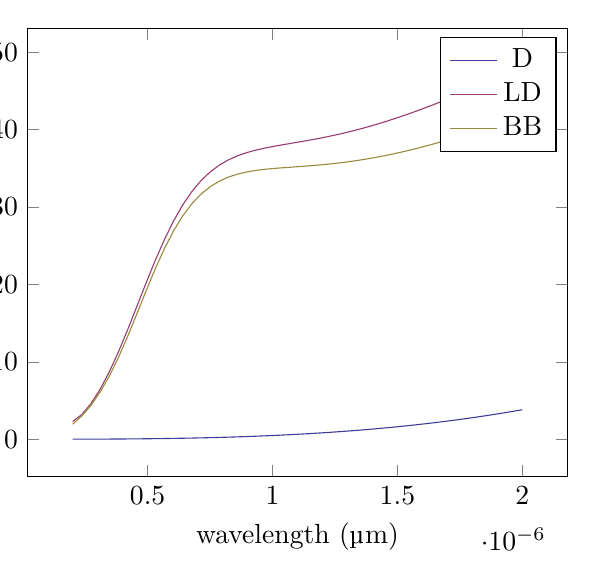
\begin{tikzpicture}[baseline,trim axis left]
			\begin{axis}[xlabel=wavelength (\si{\micro\meter}),ylabel=permittivity $\epsilon''$]
				\addplot[color=colora] coordinates {
						(2e-07, 0.0038299232976884705)
						(2.3673469387755102e-07, 0.006351492728290801)
						(2.7346938775510205e-07, 0.009790492451400486)
						(3.1020408163265303e-07, 0.01428918720821626)
						(3.4693877551020406e-07, 0.019989800657976748)
						(3.836734693877551e-07, 0.027034509869537468)
						(4.2040816326530607e-07, 0.035565439816739736)
						(4.571428571428571e-07, 0.04572465787801874)
						(4.938775510204081e-07, 0.05765416834069726)
						(5.306122448979591e-07, 0.07149590691041142)
						(5.673469387755102e-07, 0.08739173522611356)
						(6.040816326530612e-07, 0.10548343538109649)
						(6.408163265306121e-07, 0.12591270445048355)
						(6.775510204081632e-07, 0.1488211490256265)
						(7.142857142857142e-07, 0.17435027975585365)
						(7.510204081632653e-07, 0.20264150589800853)
						(7.877551020408163e-07, 0.23383612987421928)
						(8.244897959183672e-07, 0.2680753418383373)
						(8.612244897959183e-07, 0.3055002142514822)
						(8.979591836734693e-07, 0.34625169646712867)
						(9.346938775510204e-07, 0.3904706093261725)
						(9.714285714285713e-07, 0.4382976397624052)
						(1.0081632653061223e-06, 0.48987333541883404)
						(1.0448979591836734e-06, 0.5453380992752715)
						(1.0816326530612245e-06, 0.6048321842876323)
						(1.1183673469387754e-06, 0.668495688039352)
						(1.1551020408163265e-06, 0.7364685474053708)
						(1.1918367346938776e-06, 0.8088905332290854)
						(1.2285714285714284e-06, 0.8859012450127097)
						(1.2653061224489795e-06, 0.9676401056214537)
						(1.3020408163265306e-06, 1.0542463560019415)
						(1.3387755102040815e-06, 1.1458590499152852)
						(1.3755102040816325e-06, 1.2426170486852304)
						(1.4122448979591836e-06, 1.3446590159617824)
						(1.4489795918367345e-06, 1.4521234125007225)
						(1.4857142857142856e-06, 1.5651484909594358)
						(1.5224489795918367e-06, 1.683872290709429)
						(1.5591836734693875e-06, 1.8084326326659703)
						(1.5959183673469386e-06, 1.938967114135233)
						(1.6326530612244897e-06, 2.075613103679355)
						(1.6693877551020408e-06, 2.2185077359997925)
						(1.7061224489795917e-06, 2.3677879068393928)
						(1.7428571428571427e-06, 2.5235902679035322)
						(1.7795918367346938e-06, 2.6860512218007564)
						(1.8163265306122447e-06, 2.855306917003267)
						(1.8530612244897958e-06, 3.0314932428276755)
						(1.8897959183673469e-06, 3.214745824436365)
						(1.9265306122448977e-06, 3.405200017859872)
						(1.963265306122449e-06, 3.602990905040654)
						(2e-06, 3.808253288898592)
					};
				\addlegendentry{D}
				\addplot[color=colorb] coordinates {
						(2e-07, 2.2870948999275273)
						(2.3673469387755102e-07, 3.184044194898663)
						(2.7346938775510205e-07, 4.606882634813675)
						(3.1020408163265303e-07, 6.461941368100702)
						(3.4693877551020406e-07, 8.712668819194517)
						(3.836734693877551e-07, 11.305735476585639)
						(4.2040816326530607e-07, 14.157649811410613)
						(4.571428571428571e-07, 17.157096145780805)
						(4.938775510204081e-07, 20.17667107676355)
						(5.306122448979591e-07, 23.090000501314822)
						(5.673469387755102e-07, 25.789047652992515)
						(6.040816326530612e-07, 28.196620170195793)
						(6.408163265306121e-07, 30.27130579162779)
						(6.775510204081632e-07, 32.005080680652554)
						(7.142857142857142e-07, 33.416030884972166)
						(7.510204081632653e-07, 34.539252490189114)
						(7.877551020408163e-07, 35.41835815298438)
						(8.244897959183672e-07, 36.09889291183221)
						(8.612244897959183e-07, 36.6239755931106)
						(8.979591836734693e-07, 37.03188659824061)
						(9.346938775510204e-07, 37.355092062759375)
						(9.714285714285713e-07, 37.62019434795278)
						(1.0081632653061223e-06, 37.84840182802024)
						(1.0448979591836734e-06, 38.056235208355204)
						(1.0816326530612245e-06, 38.25629450794726)
						(1.1183673469387754e-06, 38.4579890415986)
						(1.1551020408163265e-06, 38.66818412017443)
						(1.1918367346938776e-06, 38.89174906899772)
						(1.2285714285714284e-06, 39.13200807152035)
						(1.2653061224489795e-06, 39.39110347835468)
						(1.3020408163265306e-06, 39.67028422883381)
						(1.3387755102040815e-06, 39.970132270613405)
						(1.3755102040816325e-06, 40.29073876142883)
						(1.4122448979591836e-06, 40.631840212513055)
						(1.4489795918367345e-06, 40.99292302153121)
						(1.4857142857142856e-06, 41.37330325574449)
						(1.5224489795918367e-06, 41.77218716882164)
						(1.5591836734693875e-06, 42.18871678577797)
						(1.5959183673469386e-06, 42.62200395600377)
						(1.6326530612244897e-06, 43.07115552694094)
						(1.6693877551020408e-06, 43.535291700044894)
						(1.7061224489795917e-06, 44.013559167139775)
						(1.7428571428571427e-06, 44.50514026362804)
						(1.7795918367346938e-06, 45.00925909388137)
						(1.8163265306122447e-06, 45.52518536610563)
						(1.8530612244897958e-06, 46.05223650512514)
						(1.8897959183673469e-06, 46.5897784808777)
						(1.9265306122448977e-06, 47.13722568935575)
						(1.963265306122449e-06, 47.69404014457081)
						(2e-06, 48.2597301796716)
					};
				\addlegendentry{LD}
				\addplot[color=colorc] coordinates {
						(2e-07, 1.9351182447360329)
						(2.3673469387755102e-07, 3.002047805601073)
						(2.7346938775510205e-07, 4.379254169469286)
						(3.1020408163265303e-07, 6.096116705845388)
						(3.4693877551020406e-07, 8.168811883702206)
						(3.836734693877551e-07, 10.586586491037934)
						(4.2040816326530607e-07, 13.296878759354156)
						(4.571428571428571e-07, 16.19838701684291)
						(4.938775510204081e-07, 19.15113239619416)
						(5.306122448979591e-07, 22.003376662349957)
						(5.673469387755102e-07, 24.623430304625664)
						(6.040816326530612e-07, 26.921873454707477)
						(6.408163265306121e-07, 28.857754571677553)
						(6.775510204081632e-07, 30.431737976224447)
						(7.142857142857142e-07, 31.673163658171287)
						(7.510204081632653e-07, 32.626918047145736)
						(7.877551020408163e-07, 33.34317071157858)
						(8.244897959183672e-07, 33.87068741971313)
						(8.612244897959183e-07, 34.25319641412518)
						(8.979591836734693e-07, 34.52790797613209)
						(9.346938775510204e-07, 34.725353405527336)
						(9.714285714285713e-07, 34.86992470894304)
						(1.0081632653061223e-06, 34.980713457277176)
						(1.0448979591836734e-06, 35.07241486833451)
						(1.0816326530612245e-06, 35.15617582916757)
						(1.1183673469387754e-06, 35.24033438008289)
						(1.1551020408163265e-06, 35.331036779097886)
						(1.1918367346938776e-06, 35.432737875953165)
						(1.2285714285714284e-06, 35.54859902762868)
						(1.2653061224489795e-06, 35.68080023028847)
						(1.3020408163265306e-06, 35.830782555545284)
						(1.3387755102040815e-06, 35.99943508119039)
						(1.3755102040816325e-06, 36.18723821715212)
						(1.4122448979591836e-06, 36.39437310019075)
						(1.4489795918367345e-06, 36.62080476112772)
						(1.4857142857142856e-06, 36.86634511563598)
						(1.5224489795918367e-06, 37.13070048671096)
						(1.5591836734693875e-06, 37.41350729834754)
						(1.5959183673469386e-06, 37.71435874145021)
						(1.6326530612244897e-06, 38.032824561272996)
						(1.6693877551020408e-06, 38.368465612378266)
						(1.7061224489795917e-06, 38.72084444010134)
						(1.7428571428571427e-06, 39.08953285075616)
						(1.7795918367346938e-06, 39.47411720566457)
						(1.8163265306122447e-06, 39.87420200037176)
						(1.8530612244897958e-06, 40.289412157596736)
						(1.8897959183673469e-06, 40.719394360932824)
						(1.9265306122448977e-06, 41.16381767865906)
						(1.963265306122449e-06, 41.622373667619215)
						(2e-06, 42.09477610165013)
					};
				\addlegendentry{BB}
			\end{axis}
		\end{tikzpicture}%
		\\
		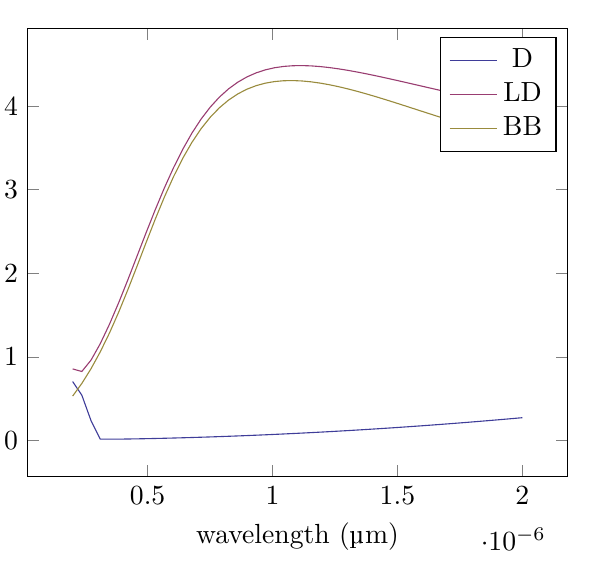
\begin{tikzpicture}[baseline,trim axis left]
			\begin{axis}[xlabel=wavelength (\si{\micro\meter}),ylabel=refractive index $n'$]
				\addplot[color=colora] coordinates {
						(2e-07, 0.7034542400401501)
						(2.3673469387755102e-07, 0.5406296641992581)
						(2.7346938775510205e-07, 0.23666379027871157)
						(3.1020408163265303e-07, 0.015394717262196595)
						(3.4693877551020406e-07, 0.013858782370402108)
						(3.836734693877551e-07, 0.014584675535115067)
						(4.2040816326530607e-07, 0.016021743939410804)
						(4.571428571428571e-07, 0.017858583424709445)
						(4.938775510204081e-07, 0.019988479553597442)
						(5.306122448979591e-07, 0.022364540435688987)
						(5.673469387755102e-07, 0.02496283929512101)
						(6.040816326530612e-07, 0.02776986627439724)
						(6.408163265306121e-07, 0.03077740871536511)
						(6.775510204081632e-07, 0.033980182908257925)
						(7.142857142857142e-07, 0.037374631925443706)
						(7.510204081632653e-07, 0.0409582699047778)
						(7.877551020408163e-07, 0.04472930326044833)
						(8.244897959183672e-07, 0.048686401341410654)
						(8.612244897959183e-07, 0.05282855202185827)
						(8.979591836734693e-07, 0.05715496769697937)
						(9.346938775510204e-07, 0.06166502231735046)
						(9.714285714285713e-07, 0.06635820815341126)
						(1.0081632653061223e-06, 0.07123410545422365)
						(1.0448979591836734e-06, 0.07629236074076041)
						(1.0816326530612245e-06, 0.08153267100754867)
						(1.1183673469387754e-06, 0.08695477204597721)
						(1.1551020408163265e-06, 0.09255842969324139)
						(1.1918367346938776e-06, 0.09834343319065562)
						(1.2285714285714284e-06, 0.10430959008477562)
						(1.2653061224489795e-06, 0.11045672227159195)
						(1.3020408163265306e-06, 0.11678466289783164)
						(1.3387755102040815e-06, 0.12329325391206902)
						(1.3755102040816325e-06, 0.1299823441133413)
						(1.4122448979591836e-06, 0.1368517875845775)
						(1.4489795918367345e-06, 0.14390144242584615)
						(1.4857142857142856e-06, 0.15113116972354956)
						(1.5224489795918367e-06, 0.15854083270634287)
						(1.5591836734693875e-06, 0.16613029605013027)
						(1.5959183673469386e-06, 0.17389942530281516)
						(1.6326530612244897e-06, 0.18184808640574762)
						(1.6693877551020408e-06, 0.18997614529390486)
						(1.7061224489795917e-06, 0.198283467560349)
						(1.7428571428571427e-06, 0.20676991817363752)
						(1.7795918367346938e-06, 0.21543536123880874)
						(1.8163265306122447e-06, 0.22427965979478653)
						(1.8530612244897958e-06, 0.23330267564191345)
						(1.8897959183673469e-06, 0.24250426919486567)
						(1.9265306122448977e-06, 0.2518842993568995)
						(1.963265306122449e-06, 0.26144262341203306)
						(2e-06, 0.2711790969325882)
					};
				\addlegendentry{D}
				\addplot[color=colorb] coordinates {
						(2e-07, 0.854617897378882)
						(2.3673469387755102e-07, 0.8241867934850218)
						(2.7346938775510205e-07, 0.9597246278138245)
						(3.1020408163265303e-07, 1.1550392860443965)
						(3.4693877551020406e-07, 1.3864490912367569)
						(3.836734693877551e-07, 1.6432761570667245)
						(4.2040816326530607e-07, 1.917236392812552)
						(4.571428571428571e-07, 2.2001728386606407)
						(4.938775510204081e-07, 2.4838117831862205)
						(5.306122448979591e-07, 2.7602099857790234)
						(5.673469387755102e-07, 3.022391018511698)
						(6.040816326530612e-07, 3.264880738243686)
						(6.408163265306121e-07, 3.483985317060307)
						(6.775510204081632e-07, 3.6777811548908157)
						(7.142857142857142e-07, 3.845880070601639)
						(7.510204081632653e-07, 3.9890739313802954)
						(7.877551020408163e-07, 4.108956071956498)
						(8.244897959183672e-07, 4.20758504964197)
						(8.612244897959183e-07, 4.2872213080981405)
						(8.979591836734693e-07, 4.350141224691523)
						(9.346938775510204e-07, 4.398518467048004)
						(9.714285714285713e-07, 4.434357195251293)
						(1.0081632653061223e-06, 4.459461755493749)
						(1.0448979591836734e-06, 4.475430112057444)
						(1.0816326530612245e-06, 4.483661489486536)
						(1.1183673469387754e-06, 4.485371625286431)
						(1.1551020408163265e-06, 4.481611341267504)
						(1.1918367346938776e-06, 4.47328581055379)
						(1.2285714285714284e-06, 4.461173032442193)
						(1.2653061224489795e-06, 4.445940761583175)
						(1.3020408163265306e-06, 4.428161590648889)
						(1.3387755102040815e-06, 4.408326149868372)
						(1.3755102040816325e-06, 4.386854529739037)
						(1.4122448979591836e-06, 4.364106100950891)
						(1.4489795918367345e-06, 4.340387928534017)
						(1.4857142857142856e-06, 4.315961974986095)
						(1.5224489795918367e-06, 4.291051271832439)
						(1.5591836734693875e-06, 4.2658452180891135)
						(1.5959183673469386e-06, 4.240504141736934)
						(1.6326530612244897e-06, 4.21516323893619)
						(1.6693877551020408e-06, 4.18993598649434)
						(1.7061224489795917e-06, 4.164917106501565)
						(1.7428571428571427e-06, 4.1401851481156)
						(1.7795918367346938e-06, 4.1158047400241635)
						(1.8163265306122447e-06, 4.091828557846174)
						(1.8530612244897958e-06, 4.068299043319047)
						(1.8897959183673469e-06, 4.045249906229162)
						(1.9265306122448977e-06, 4.022707435374588)
						(1.963265306122449e-06, 4.000691641140441)
						(2e-06, 3.9792172492983284)
					};
				\addlegendentry{LD}
				\addplot[color=colorc] coordinates {
						(2e-07, 0.5295291493111692)
						(2.3673469387755102e-07, 0.681085920414362)
						(2.7346938775510205e-07, 0.8568136491272005)
						(3.1020408163265303e-07, 1.05694882292993)
						(3.4693877551020406e-07, 1.281697259774658)
						(3.836734693877551e-07, 1.5299568368628074)
						(4.2040816326530607e-07, 1.79818997847309)
						(4.571428571428571e-07, 2.0798796469499243)
						(4.938775510204081e-07, 2.3660367453921176)
						(5.306122448979591e-07, 2.6467040018347987)
						(5.673469387755102e-07, 2.912765139458195)
						(6.040816326530612e-07, 3.1572727575721404)
						(6.408163265306121e-07, 3.3759509222872532)
						(6.775510204081632e-07, 3.5670038568263283)
						(7.142857142857142e-07, 3.7305584437905086)
						(7.510204081632653e-07, 3.868027095287499)
						(7.877551020408163e-07, 3.981554391462477)
						(8.244897959183672e-07, 4.073605282827229)
						(8.612244897959183e-07, 4.146691684792154)
						(8.979591836734693e-07, 4.203209536579742)
						(9.346938775510204e-07, 4.245354266969855)
						(9.714285714285713e-07, 4.275087332136109)
						(1.0081632653061223e-06, 4.294133517068722)
						(1.0448979591836734e-06, 4.303995142732934)
						(1.0816326530612245e-06, 4.3059743046337235)
						(1.1183673469387754e-06, 4.301197775718482)
						(1.1551020408163265e-06, 4.290641527946801)
						(1.1918367346938776e-06, 4.2751532926969436)
						(1.2285714285714284e-06, 4.255472467504966)
						(1.2653061224489795e-06, 4.232247190170331)
						(1.3020408163265306e-06, 4.206048681948526)
						(1.3387755102040815e-06, 4.177383101973701)
						(1.3755102040816325e-06, 4.146701213899839)
						(1.4122448979591836e-06, 4.114406179052867)
						(1.4489795918367345e-06, 4.080859779555014)
						(1.4857142857142856e-06, 4.046387352151197)
						(1.5224489795918367e-06, 4.011281685496438)
						(1.5591836734693875e-06, 3.975806103870245)
						(1.5959183673469386e-06, 3.9401969303165134)
						(1.6326530612244897e-06, 3.904665492851407)
						(1.6693877551020408e-06, 3.8693998090862647)
						(1.7061224489795917e-06, 3.8345660577623373)
						(1.7428571428571427e-06, 3.800309920707399)
						(1.7795918367346938e-06, 3.7667578560531836)
						(1.8163265306122447e-06, 3.7340183436270493)
						(1.8530612244897958e-06, 3.702183126587256)
						(1.8897959183673469e-06, 3.671328459796421)
						(1.9265306122448977e-06, 3.641516365126638)
						(1.963265306122449e-06, 3.6127958866877745)
						(2e-06, 3.5852043345382585)
					};
				\addlegendentry{BB}
			\end{axis}
		\end{tikzpicture}%
		\\
		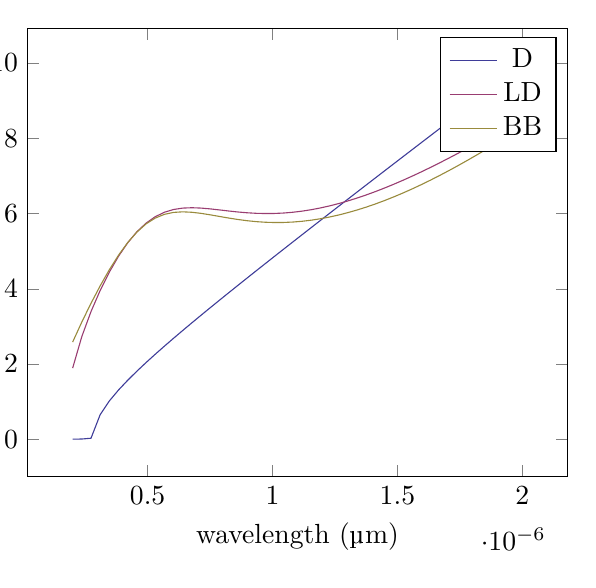
\begin{tikzpicture}[baseline,trim axis left]
			\begin{axis}[xlabel=wavelength (\si{\micro\meter}),ylabel=refractive index $n''$]
				\addplot[color=colora] coordinates {
						(2e-07, 0.0038498093849990644)
						(2.3673469387755102e-07, 0.008307319920159087)
						(2.7346938775510205e-07, 0.02925214539743523)
						(3.1020408163265303e-07, 0.6563278169054242)
						(3.4693877551020406e-07, 1.0199253601102969)
						(3.836734693877551e-07, 1.3107103554535287)
						(4.2040816326530607e-07, 1.569652078163565)
						(4.571428571428571e-07, 1.810458023688946)
						(4.938775510204081e-07, 2.039557500512219)
						(5.306122448979591e-07, 2.260508806287018)
						(5.673469387755102e-07, 2.475491183814392)
						(6.040816326530612e-07, 2.6859348807737944)
						(6.408163265306121e-07, 2.892827267489583)
						(6.775510204081632e-07, 3.0968769045213214)
						(7.142857142857142e-07, 3.298608140491314)
						(7.510204081632653e-07, 3.4984188371107385)
						(7.877551020408163e-07, 3.69661723004518)
						(8.244897959183672e-07, 3.8934463599706746)
						(8.612244897959183e-07, 4.089100777583389)
						(8.979591836734693e-07, 4.283738272188317)
						(9.346938775510204e-07, 4.477488296162804)
						(9.714285714285713e-07, 4.670458137410014)
						(1.0081632653061223e-06, 4.862737521421362)
						(1.0448979591836734e-06, 5.0544020960006595)
						(1.0816326530612245e-06, 5.245516106666858)
						(1.1183673469387754e-06, 5.436134476399272)
						(1.1551020408163265e-06, 5.626304440631184)
						(1.1918367346938776e-06, 5.816066845815977)
						(1.2285714285714284e-06, 6.005457190474862)
						(1.2653061224489795e-06, 6.194506466981946)
						(1.3020408163265306e-06, 6.383241847624396)
						(1.3387755102040815e-06, 6.571687247843616)
						(1.3755102040816325e-06, 6.759863791786802)
						(1.4122448979591836e-06, 6.947790199544259)
						(1.4489795918367345e-06, 7.135483111144833)
						(1.4857142857142856e-06, 7.322957359131912)
						(1.5224489795918367e-06, 7.51022619906502)
						(1.5591836734693875e-06, 7.697301505387502)
						(1.5959183673469386e-06, 7.8841939386245095)
						(1.6326530612244897e-06, 8.07091308872271)
						(1.6693877551020408e-06, 8.257467598436486)
						(1.7061224489795917e-06, 8.443865269947583)
						(1.7428571428571427e-06, 8.630113157333142)
						(1.7795918367346938e-06, 8.816217647038712)
						(1.8163265306122447e-06, 9.002184528143259)
						(1.8530612244897958e-06, 9.188019053903815)
						(1.8897959183673469e-06, 9.373725995823415)
						(1.9265306122448977e-06, 9.55930969128647)
						(1.963265306122449e-06, 9.74477408564153)
						(2e-06, 9.930122769475846)
					};
				\addlegendentry{D}
				\addplot[color=colorb] coordinates {
						(2e-07, 1.8923314359738392)
						(2.3673469387755102e-07, 2.7317341889092304)
						(2.7346938775510205e-07, 3.3942631634115235)
						(3.1020408163265303e-07, 3.9559542400172973)
						(3.4693877551020406e-07, 4.443572608056897)
						(3.836734693877551e-07, 4.8648927250700815)
						(4.2040816326530607e-07, 5.221562779030587)
						(4.571428571428571e-07, 5.514066357412403)
						(4.938775510204081e-07, 5.744018543083114)
						(5.306122448979591e-07, 5.915164431764215)
						(5.673469387755102e-07, 6.03350471996628)
						(6.040816326530612e-07, 6.106814590603488)
						(6.408163265306121e-07, 6.14383921074978)
						(6.775510204081632e-07, 6.153441063674122)
						(7.142857142857142e-07, 6.143899863056966)
						(7.510204081632653e-07, 6.122458513692241)
						(7.877551020408163e-07, 6.095115350440828)
						(8.244897959183672e-07, 6.066608676978632)
						(8.612244897959183e-07, 6.040523601378381)
						(8.979591836734693e-07, 6.019459318956714)
						(9.346938775510204e-07, 6.005212688615194)
						(9.714285714285713e-07, 5.998951677027844)
						(1.0081632653061223e-06, 6.001365872618246)
						(1.0448979591836734e-06, 6.012790124855113)
						(1.0816326530612245e-06, 6.033302320674762)
						(1.1183673469387754e-06, 6.062798607099969)
						(1.1551020408163265e-06, 6.101050074505614)
						(1.1918367346938776e-06, 6.147744781702047)
						(1.2285714285714284e-06, 6.202518500760998)
						(1.2653061224489795e-06, 6.264976949006185)
						(1.3020408163265306e-06, 6.334711689167515)
						(1.3387755102040815e-06, 6.411311371396126)
						(1.3755102040816325e-06, 6.4943695771276895)
						(1.4122448979591836e-06, 6.583490199767611)
						(1.4489795918367345e-06, 6.678291048278055)
						(1.4857142857142856e-06, 6.778406172662966)
						(1.5224489795918367e-06, 6.8834872717458575)
						(1.5591836734693875e-06, 6.993204442177475)
						(1.5959183673469386e-06, 7.107246454122152)
						(1.6326530612244897e-06, 7.225320686353004)
						(1.6693877551020408e-06, 7.347152816001082)
						(1.7061224489795917e-06, 7.472486331758443)
						(1.7428571428571427e-06, 7.601081920791228)
						(1.7795918367346938e-06, 7.732716766655686)
						(1.8163265306122447e-06, 7.867183786432249)
						(1.8530612244897958e-06, 8.00429082888018)
						(1.8897959183673469e-06, 8.143859850803848)
						(1.9265306122448977e-06, 8.285726085412037)
						(1.963265306122449e-06, 8.429737213837312)
						(2e-06, 8.575752548895446)
					};
				\addlegendentry{LD}
				\addplot[color=colorc] coordinates {
						(2e-07, 2.5840602637846057)
						(2.3673469387755102e-07, 3.11674092381069)
						(2.7346938775510205e-07, 3.614088457770915)
						(3.1020408163265303e-07, 4.078348325000824)
						(3.4693877551020406e-07, 4.506697843934403)
						(3.836734693877551e-07, 4.892848554329564)
						(4.2040816326530607e-07, 5.228765176045829)
						(4.571428571428571e-07, 5.507044275706363)
						(4.938775510204081e-07, 5.723451088037097)
						(5.306122448979591e-07, 5.878533011686819)
						(5.673469387755102e-07, 5.977617044577046)
						(6.040816326530612e-07, 6.0294566683901065)
						(6.408163265306121e-07, 6.0443751752247845)
						(6.775510204081632e-07, 6.0326506922888905)
						(7.142857142857142e-07, 6.003473512552189)
						(7.510204081632653e-07, 5.964465716504946)
						(7.877551020408163e-07, 5.921602419139044)
						(8.244897959183672e-07, 5.879360196947393)
						(8.612244897959183e-07, 5.840961735971615)
						(8.979591836734693e-07, 5.808636866097121)
						(9.346938775510204e-07, 5.783859562248896)
						(9.714285714285713e-07, 5.767545386923795)
						(1.0081632653061223e-06, 5.760207408098707)
						(1.0448979591836734e-06, 5.762074901004618)
						(1.0816326530612245e-06, 5.7731812989779465)
						(1.1183673469387754e-06, 5.793427949793722)
						(1.1551020408163265e-06, 5.82262944366887)
						(1.1918367346938776e-06, 5.86054522790839)
						(1.2285714285714284e-06, 5.906901202172661)
						(1.2653061224489795e-06, 5.961404111649747)
						(1.3020408163265306e-06, 6.023750849338549)
						(1.3387755102040815e-06, 6.093634230666466)
						(1.3755102040816325e-06, 6.170746387511324)
						(1.4122448979591836e-06, 6.254780616264352)
						(1.4489795918367345e-06, 6.3454322809213615)
						(1.4857142857142856e-06, 6.4423991971433185)
						(1.5224489795918367e-06, 6.545381791383863)
						(1.5591836734693875e-06, 6.654083229280472)
						(1.5959183673469386e-06, 6.7682096316032)
						(1.6326530612244897e-06, 6.8874704386816585)
						(1.6693877551020408e-06, 7.011578941655619)
						(1.7061224489795917e-06, 7.140252968504749)
						(1.7428571428571427e-06, 7.273215692639859)
						(1.7795918367346938e-06, 7.410196520230974)
						(1.8163265306122447e-06, 7.550932007869427)
						(1.8530612244897958e-06, 7.695166763108775)
						(1.8897959183673469e-06, 7.842654285424919)
						(1.9265306122448977e-06, 7.993157712774487)
						(1.963265306122449e-06, 8.14645044794845)
						(2e-06, 8.302316648247539)
					};
				\addlegendentry{BB}
			\end{axis}
		\end{tikzpicture}%
		\\
	\end{tabular}
	\caption{Complex permittivity $\epsilon = \epsilon' + \mi \epsilon''$ and refractive index $n = n' + \mi n''$ for Cr based on the Drude (D), Lorentz-Drude (LD), and Brendel-Bormann (BB) models.}
\end{figure}
\clearpage
\newpage
\subsection{Ni}
\begin{figure}[h!]
	\centering
	\begin{tabular}{l}
		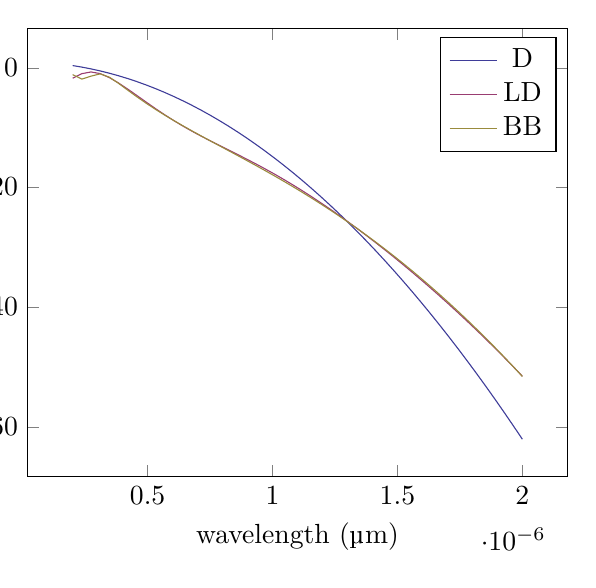
\begin{tikzpicture}[baseline,trim axis left]
			\begin{axis}[xlabel=wavelength (\si{\micro\meter}),ylabel=permittivity $\epsilon'$]
				\addplot[color=colora] coordinates {
						(2e-07, 0.36691993611761264)
						(2.3673469387755102e-07, 0.11302368648159411)
						(2.7346938775510205e-07, -0.18356861920452316)
						(3.1020408163265303e-07, -0.5228497845648341)
						(3.4693877551020406e-07, -0.9048115781847013)
						(3.836734693877551e-07, -1.3294447341099245)
						(4.2040816326530607e-07, -1.796738952408568)
						(4.571428571428571e-07, -2.306682899795382)
						(4.938775510204081e-07, -2.859264210318732)
						(5.306122448979591e-07, -3.454469486109983)
						(5.673469387755102e-07, -4.092284298195237)
						(6.040816326530612e-07, -4.772693187369327)
						(6.408163265306121e-07, -5.4956796651319895)
						(6.775510204081632e-07, -6.261226214686095)
						(7.142857142857142e-07, -7.069314291997825)
						(7.510204081632653e-07, -7.919924326918668)
						(7.877551020408163e-07, -8.81303572436914)
						(8.244897959183672e-07, -9.748626865584052)
						(8.612244897959183e-07, -10.726675109419224)
						(8.979591836734693e-07, -11.747156793719446)
						(9.346938775510204e-07, -12.810047236747621)
						(9.714285714285713e-07, -13.9153207386748)
						(1.0081632653061223e-06, -15.062950583131123)
						(1.0448979591836734e-06, -16.252909038817226)
						(1.0816326530612245e-06, -17.48516736117628)
						(1.1183673469387754e-06, -18.759695794126092)
						(1.1551020408163265e-06, -20.076463571851452)
						(1.1918367346938776e-06, -21.435438920656175)
						(1.2285714285714284e-06, -22.8365890608749)
						(1.2653061224489795e-06, -24.2798802088443)
						(1.3020408163265306e-06, -25.765277578933503)
						(1.3387755102040815e-06, -27.292745385633463)
						(1.3755102040816325e-06, -28.8622468457052)
						(1.4122448979591836e-06, -30.47374418038642)
						(1.4489795918367345e-06, -32.12719861765647)
						(1.4857142857142856e-06, -33.822570394559385)
						(1.5224489795918367e-06, -35.55981875958452)
						(1.5591836734693875e-06, -37.33890197510485)
						(1.5959183673469386e-06, -39.15977731987233)
						(1.6326530612244897e-06, -41.02240109157044)
						(1.6693877551020408e-06, -42.92672860942301)
						(1.7061224489795917e-06, -44.872714216859876)
						(1.7428571428571427e-06, -46.86031128423828)
						(1.7795918367346938e-06, -48.889472211620124)
						(1.8163265306122447e-06, -50.96014843160475)
						(1.8530612244897958e-06, -53.072290412216915)
						(1.8897959183673469e-06, -55.22584765984943)
						(1.9265306122448977e-06, -57.42076872226042)
						(1.963265306122449e-06, -59.65700119162493)
						(2e-06, -61.934491707640014)
					};
				\addlegendentry{D}
				\addplot[color=colorb] coordinates {
						(2e-07, -1.7423228818063747)
						(2.3673469387755102e-07, -0.982211050556822)
						(2.7346938775510205e-07, -0.6947871184657146)
						(3.1020408163265303e-07, -0.9718950057818658)
						(3.4693877551020406e-07, -1.6365605114035453)
						(3.836734693877551e-07, -2.529865920259179)
						(4.2040816326530607e-07, -3.5476378069531718)
						(4.571428571428571e-07, -4.622757510779872)
						(4.938775510204081e-07, -5.7099738853080115)
						(5.306122448979591e-07, -6.7780398438811496)
						(5.673469387755102e-07, -7.806238916463137)
						(6.040816326530612e-07, -8.782827960798215)
						(6.408163265306121e-07, -9.703974521157521)
						(6.775510204081632e-07, -10.572517837944176)
						(7.142857142857142e-07, -11.396377952105597)
						(7.510204081632653e-07, -12.186737070468293)
						(7.877551020408163e-07, -12.956245226876927)
						(8.244897959183672e-07, -13.717491991161424)
						(8.612244897959183e-07, -14.481893808926522)
						(8.979591836734693e-07, -15.259033712012227)
						(9.346938775510204e-07, -16.056400739889405)
						(9.714285714285713e-07, -16.87942839754423)
						(1.0081632653061223e-06, -17.731721603921212)
						(1.0448979591836734e-06, -18.615376455499153)
						(1.0816326530612245e-06, -19.531322596295013)
						(1.1183673469387754e-06, -20.47964394130547)
						(1.1551020408163265e-06, -21.4598547103232)
						(1.1918367346938776e-06, -22.471122655136252)
						(1.2285714285714284e-06, -23.51244055430238)
						(1.2653061224489795e-06, -24.582751874498975)
						(1.3020408163265306e-06, -25.681038395658625)
						(1.3387755102040815e-06, -26.806377748049027)
						(1.3755102040816325e-06, -27.957978051831933)
						(1.4122448979591836e-06, -29.135195719897602)
						(1.4489795918367345e-06, -30.337541293343342)
						(1.4857142857142856e-06, -31.564677084736857)
						(1.5224489795918367e-06, -32.81640947314172)
						(1.5591836734693875e-06, -34.092677940335605)
						(1.5959183673469386e-06, -35.393542346963144)
						(1.6326530612244897e-06, -36.71916949688839)
						(1.6693877551020408e-06, -38.06981970166583)
						(1.7061224489795917e-06, -39.44583381050162)
						(1.7428571428571427e-06, -40.84762099345032)
						(1.7795918367346938e-06, -42.275647439867214)
						(1.8163265306122447e-06, -43.73042604688391)
						(1.8530612244897958e-06, -45.212507113559894)
						(1.8897959183673469e-06, -46.722470017565996)
						(1.9265306122448977e-06, -48.26091582694562)
						(1.963265306122449e-06, -49.82846078537556)
						(2e-06, -51.425730602271315)
					};
				\addlegendentry{LD}
				\addplot[color=colorc] coordinates {
						(2e-07, -1.1350628069064994)
						(2.3673469387755102e-07, -1.8881247906738197)
						(2.7346938775510205e-07, -1.3974935314090475)
						(3.1020408163265303e-07, -1.0136150767233487)
						(3.4693877551020406e-07, -1.569969778561592)
						(3.836734693877551e-07, -2.5950963670156257)
						(4.2040816326530607e-07, -3.7269663548488445)
						(4.571428571428571e-07, -4.838976947483527)
						(4.938775510204081e-07, -5.899153703185284)
						(5.306122448979591e-07, -6.904840756835173)
						(5.673469387755102e-07, -7.861839325859372)
						(6.040816326530612e-07, -8.778082479026155)
						(6.408163265306121e-07, -9.661653290816199)
						(6.775510204081632e-07, -10.52014311711909)
						(7.142857142857142e-07, -11.360455130799359)
						(7.510204081632653e-07, -12.188769080054193)
						(7.877551020408163e-07, -13.01056887946153)
						(8.244897959183672e-07, -13.83069523333302)
						(8.612244897959183e-07, -14.65340709151381)
						(8.979591836734693e-07, -15.482444311315227)
						(9.346938775510204e-07, -16.321087740746158)
						(9.714285714285713e-07, -17.17221486997766)
						(1.0081632653061223e-06, -18.03835025649724)
						(1.0448979591836734e-06, -18.921710535434393)
						(1.0816326530612245e-06, -19.824244173685827)
						(1.1183673469387754e-06, -20.747666316319783)
						(1.1551020408163265e-06, -21.69348916566559)
						(1.1918367346938776e-06, -22.663048364691498)
						(1.2285714285714284e-06, -23.657525850804372)
						(1.2653061224489795e-06, -24.677969619796613)
						(1.3020408163265306e-06, -25.72531080248241)
						(1.3387755102040815e-06, -26.800378415063662)
						(1.3755102040816325e-06, -27.90391210239784)
						(1.4122448979591836e-06, -29.036573153406174)
						(1.4489795918367345e-06, -30.198954031082973)
						(1.4857142857142856e-06, -31.391586626480752)
						(1.5224489795918367e-06, -32.61494941676287)
						(1.5591836734693875e-06, -33.869473681802624)
						(1.5959183673469386e-06, -35.15554891159235)
						(1.6326530612244897e-06, -36.47352751757986)
						(1.6693877551020408e-06, -37.8237289446209)
						(1.7061224489795917e-06, -39.20644326618518)
						(1.7428571428571427e-06, -40.62193433346431)
						(1.7795918367346938e-06, -42.07044253881315)
						(1.8163265306122447e-06, -43.5521872452579)
						(1.8530612244897958e-06, -45.067368926403056)
						(1.8897959183673469e-06, -46.61617105476808)
						(1.9265306122448977e-06, -48.19876177122321)
						(1.963265306122449e-06, -49.81529536362359)
						(2e-06, -51.465913578847164)
					};
				\addlegendentry{BB}
			\end{axis}
		\end{tikzpicture}%
		\\
		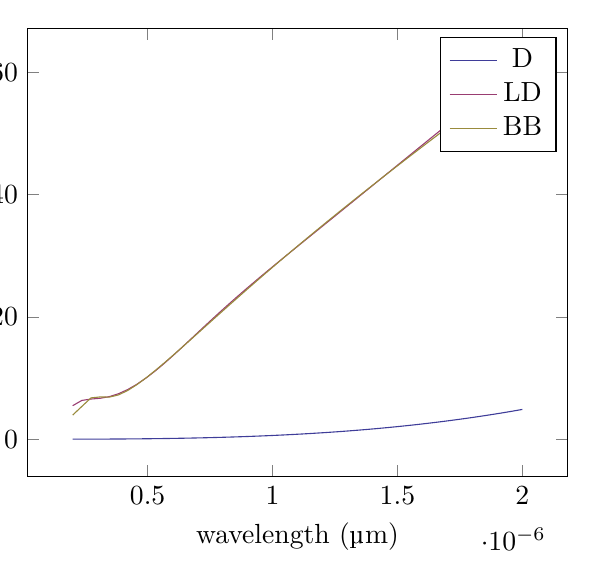
\begin{tikzpicture}[baseline,trim axis left]
			\begin{axis}[xlabel=wavelength (\si{\micro\meter}),ylabel=permittivity $\epsilon''$]
				\addplot[color=colora] coordinates {
						(2e-07, 0.004901889668259111)
						(2.3673469387755102e-07, 0.008129219124795476)
						(2.7346938775510205e-07, 0.012530749811679514)
						(3.1020408163265303e-07, 0.01828855837521647)
						(3.4693877551020406e-07, 0.025584666621623838)
						(3.836734693877551e-07, 0.03460103416444393)
						(4.2040816326530607e-07, 0.04551955107723571)
						(4.571428571428571e-07, 0.058522030552168494)
						(4.938775510204081e-07, 0.07379020156513898)
						(5.306122448979591e-07, 0.09150570154803302)
						(5.673469387755102e-07, 0.11185006906875107)
						(6.040816326530612e-07, 0.13500473651961672)
						(6.408163265306121e-07, 0.16115102281478505)
						(6.775510204081632e-07, 0.1904701260972678)
						(7.142857142857142e-07, 0.2231431164561888)
						(7.510204081632653e-07, 0.259350928654884)
						(7.877551020408163e-07, 0.2992743548704576)
						(8.244897959183672e-07, 0.3430940374454034)
						(8.612244897959183e-07, 0.3909904616519013)
						(8.979591836734693e-07, 0.4431439484693918)
						(9.346938775510204e-07, 0.4997346473760396)
						(9.714285714285713e-07, 0.5609425291546799)
						(1.0081632653061223e-06, 0.6269473787138578)
						(1.0448979591836734e-06, 0.6979287879245473)
						(1.0816326530612245e-06, 0.7740661484731599)
						(1.1183673469387754e-06, 0.8555386447314196)
						(1.1551020408163265e-06, 0.9425252466437163)
						(1.1918367346938776e-06, 1.035204702632502)
						(1.2285714285714284e-06, 1.133755532522336)
						(1.2653061224489795e-06, 1.2383560204831563)
						(1.3020408163265306e-06, 1.34918420799335)
						(1.3387755102040815e-06, 1.4664178868232083)
						(1.3755102040816325e-06, 1.5902345920393484)
						(1.4122448979591836e-06, 1.7208115950306482)
						(1.4489795918367345e-06, 1.8583258965562932)
						(1.4857142857142856e-06, 2.0029542198164894)
						(1.5224489795918367e-06, 2.1548730035463852)
						(1.5591836734693875e-06, 2.3142583951337965)
						(1.5959183673469386e-06, 2.4812862437612653)
						(1.6326530612244897e-06, 2.6561320935730115)
						(1.6693877551020408e-06, 2.838971176867321)
						(1.7061224489795917e-06, 3.02997840731494)
						(1.7428571428571427e-06, 3.2293283732039697)
						(1.7795918367346938e-06, 3.4371953307118486)
						(1.8163265306122447e-06, 3.6537531972049204)
						(1.8530612244897958e-06, 3.8791755445661433)
						(1.8897959183673469e-06, 4.1136355925514385)
						(1.9265306122448977e-06, 4.357306202175221)
						(1.963265306122449e-06, 4.610359869125645)
						(2e-06, 4.872968717210017)
					};
				\addlegendentry{D}
				\addplot[color=colorb] coordinates {
						(2e-07, 5.483166660730304)
						(2.3673469387755102e-07, 6.344414133193281)
						(2.7346938775510205e-07, 6.573917947476577)
						(3.1020408163265303e-07, 6.70059027103988)
						(3.4693877551020406e-07, 6.969759495492944)
						(3.836734693877551e-07, 7.445058134793111)
						(4.2040816326530607e-07, 8.125431172314128)
						(4.571428571428571e-07, 8.990834786213714)
						(4.938775510204081e-07, 10.015644493834795)
						(5.306122448979591e-07, 11.172098410192689)
						(5.673469387755102e-07, 12.431481201194202)
						(6.040816326530612e-07, 13.765244719402258)
						(6.408163265306121e-07, 15.146426635540932)
						(6.775510204081632e-07, 16.551138265679835)
						(7.142857142857142e-07, 17.95977180066087)
						(7.510204081632653e-07, 19.357668883793636)
						(7.877551020408163e-07, 20.73516781435409)
						(8.244897959183672e-07, 22.087113083992996)
						(8.612244897959183e-07, 23.41201244181854)
						(8.979591836734693e-07, 24.71105006168851)
						(9.346938775510204e-07, 25.987129102849142)
						(9.714285714285713e-07, 27.244054815156645)
						(1.0081632653061223e-06, 28.4859074328494)
						(1.0448979591836734e-06, 29.716607437737217)
						(1.0816326530612245e-06, 30.93964815668252)
						(1.1183673469387754e-06, 32.157959146108794)
						(1.1551020408163265e-06, 33.373863067949394)
						(1.1918367346938776e-06, 34.58909374693726)
						(1.2285714285714284e-06, 35.80485018833723)
						(1.2653061224489795e-06, 37.02186837818319)
						(1.3020408163265306e-06, 38.24049866702253)
						(1.3387755102040815e-06, 39.46078114826912)
						(1.3755102040816325e-06, 40.68251475515196)
						(1.4122448979591836e-06, 41.90531804331463)
						(1.4489795918367345e-06, 43.128681058708835)
						(1.4857142857142856e-06, 44.35200854539569)
						(1.5224489795918367e-06, 45.57465521129293)
						(1.5591836734693875e-06, 46.795953980061356)
						(1.5959183673469386e-06, 48.01523821173797)
						(1.6326530612244897e-06, 49.231858839343786)
						(1.6693877551020408e-06, 50.445197286436446)
						(1.7061224489795917e-06, 51.65467492828478)
						(1.7428571428571427e-06, 52.85975975303222)
						(1.7795918367346938e-06, 54.059970777849585)
						(1.8163265306122447e-06, 55.25488068314752)
						(1.8530612244897958e-06, 56.44411704720458)
						(1.8897959183673469e-06, 57.627362494257135)
						(1.9265306122448977e-06, 58.80435401052838)
						(1.963265306122449e-06, 59.9748816337647)
						(2e-06, 61.13878668137385)
					};
				\addlegendentry{LD}
				\addplot[color=colorc] coordinates {
						(2e-07, 3.9436345127196155)
						(2.3673469387755102e-07, 5.360451533747571)
						(2.7346938775510205e-07, 6.7636971392723035)
						(3.1020408163265303e-07, 6.919729419741888)
						(3.4693877551020406e-07, 6.887598407664308)
						(3.836734693877551e-07, 7.250377582126562)
						(4.2040816326530607e-07, 7.972657163591641)
						(4.571428571428571e-07, 8.931252949980307)
						(4.938775510204081e-07, 10.039124788742958)
						(5.306122448979591e-07, 11.242478519676908)
						(5.673469387755102e-07, 12.507442380058281)
						(6.040816326530612e-07, 13.811741558671242)
						(6.408163265306121e-07, 15.140171281488023)
						(6.775510204081632e-07, 16.482084662581812)
						(7.142857142857142e-07, 17.82991491326622)
						(7.510204081632653e-07, 19.178250823670105)
						(7.877551020408163e-07, 20.52322703066735)
						(8.244897959183672e-07, 21.862105062234935)
						(8.612244897959183e-07, 23.192976661717573)
						(8.979591836734693e-07, 24.51454914074023)
						(9.346938775510204e-07, 25.825987717137686)
						(9.714285714285713e-07, 27.126798478439685)
						(1.0081632653061223e-06, 28.41674085834904)
						(1.0448979591836734e-06, 29.695761847742062)
						(1.0816326530612245e-06, 30.963946371952655)
						(1.1183673469387754e-06, 32.2214797816564)
						(1.1551020408163265e-06, 33.46861947126514)
						(1.1918367346938776e-06, 34.7056734042463)
						(1.2285714285714284e-06, 35.932983882321)
						(1.2653061224489795e-06, 37.15091530609856)
						(1.3020408163265306e-06, 38.3598449796741)
						(1.3387755102040815e-06, 39.56015623975229)
						(1.3755102040816325e-06, 40.752233361288305)
						(1.4122448979591836e-06, 41.936457821099424)
						(1.4489795918367345e-06, 43.11320559904013)
						(1.4857142857142856e-06, 44.28284527098838)
						(1.5224489795918367e-06, 45.445736704846375)
						(1.5591836734693875e-06, 46.60223021433307)
						(1.5959183673469386e-06, 47.75266605876265)
						(1.6326530612244897e-06, 48.89737420268905)
						(1.6693877551020408e-06, 50.03667426907782)
						(1.7061224489795917e-06, 51.17087563493042)
						(1.7428571428571427e-06, 52.30027763007897)
						(1.7795918367346938e-06, 53.4251698089956)
						(1.8163265306122447e-06, 54.54583227252745)
						(1.8530612244897958e-06, 55.662536021947574)
						(1.8897959183673469e-06, 56.77554333195818)
						(1.9265306122448977e-06, 57.885108132576946)
						(1.963265306122449e-06, 58.99147639238841)
						(2e-06, 60.09488649761909)
					};
				\addlegendentry{BB}
			\end{axis}
		\end{tikzpicture}%
		\\
		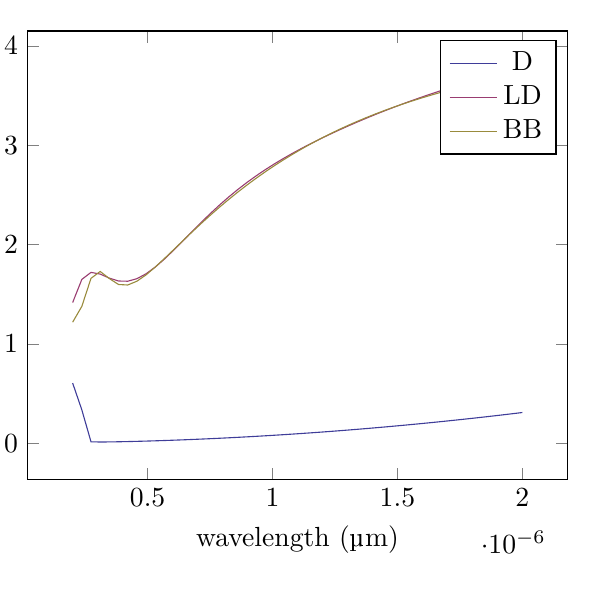
\begin{tikzpicture}[baseline,trim axis left]
			\begin{axis}[xlabel=wavelength (\si{\micro\meter}),ylabel=refractive index $n'$]
				\addplot[color=colora] coordinates {
						(2e-07, 0.6057526782128346)
						(2.3673469387755102e-07, 0.3364070024142737)
						(2.7346938775510205e-07, 0.014614882354390936)
						(3.1020408163265303e-07, 0.012644295035037861)
						(3.4693877551020406e-07, 0.013447058685901384)
						(3.836734693877551e-07, 0.015003313207819705)
						(4.2040816326530607e-07, 0.016978161018403593)
						(4.571428571428571e-07, 0.01926462273430318)
						(4.938775510204081e-07, 0.021817521353644807)
						(5.306122448979591e-07, 0.024614408135527236)
						(5.673469387755102e-07, 0.02764285015259186)
						(6.040816326530612e-07, 0.03089540033654568)
						(6.408163265306121e-07, 0.03436732278323075)
						(6.775510204081632e-07, 0.038055458254902884)
						(7.142857142857142e-07, 0.041957614162194526)
						(7.510204081632653e-07, 0.0460722163650619)
						(7.877551020408163e-07, 0.05039810050185118)
						(8.244897959183672e-07, 0.05493438176562675)
						(8.612244897959183e-07, 0.05968037080402081)
						(8.979591836734693e-07, 0.06463551778708805)
						(9.346938775510204e-07, 0.06979937424883692)
						(9.714285714285713e-07, 0.07517156646678949)
						(1.0081632653061223e-06, 0.08075177652083135)
						(1.0448979591836734e-06, 0.08653972857741976)
						(1.0816326530612245e-06, 0.09253517880003229)
						(1.1183673469387754e-06, 0.09873790782110749)
						(1.1551020408163265e-06, 0.10514771505256851)
						(1.1918367346938776e-06, 0.11176441433531605)
						(1.2285714285714284e-06, 0.11858783057677907)
						(1.2653061224489795e-06, 0.1256177971266039)
						(1.3020408163265306e-06, 0.13285415370991377)
						(1.3387755102040815e-06, 0.14029674478605622)
						(1.3755102040816325e-06, 0.14794541823525548)
						(1.4122448979591836e-06, 0.15580002430012244)
						(1.4489795918367345e-06, 0.16386041472703505)
						(1.4857142857142856e-06, 0.17212644206531177)
						(1.5224489795918367e-06, 0.18059795909193185)
						(1.5591836734693875e-06, 0.1892748183370486)
						(1.5959183673469386e-06, 0.1981568716903763)
						(1.6326530612244897e-06, 0.2072439700736212)
						(1.6693877551020408e-06, 0.21653596316646978)
						(1.7061224489795917e-06, 0.22603269917665497)
						(1.7428571428571427e-06, 0.23573402464638904)
						(1.7795918367346938e-06, 0.24563978428880326)
						(1.8163265306122447e-06, 0.2557498208495427)
						(1.8530612244897958e-06, 0.2660639749891976)
						(1.8897959183673469e-06, 0.2765820851834468)
						(1.9265306122448977e-06, 0.2873039876379798)
						(1.963265306122449e-06, 0.29822951621594995)
						(2e-06, 0.3093585023762123)
					};
				\addlegendentry{D}
				\addplot[color=colorb] coordinates {
						(2e-07, 1.4161580209110922)
						(2.3673469387755102e-07, 1.6489062190795631)
						(2.7346938775510205e-07, 1.7198465559255605)
						(3.1020408163265303e-07, 1.7027644024191273)
						(3.4693877551020406e-07, 1.6617401311742122)
						(3.836734693877551e-07, 1.632985468443669)
						(4.2040816326530607e-07, 1.630720406770916)
						(4.571428571428571e-07, 1.656334991026821)
						(4.938775510204081e-07, 1.705723729539152)
						(5.306122448979591e-07, 1.773328166539427)
						(5.673469387755102e-07, 1.8537754926896597)
						(6.040816326530612e-07, 1.9423794196252357)
						(6.408163265306121e-07, 2.0352386675966287)
						(6.775510204081632e-07, 2.129224597126468)
						(7.142857142857142e-07, 2.221940999783856)
						(7.510204081632653e-07, 2.311667504603597)
						(7.877551020408163e-07, 2.397283702806711)
						(8.244897959183672e-07, 2.4781750561617755)
						(8.612244897959183e-07, 2.5541278044309936)
						(8.979591836734693e-07, 2.625223032778507)
						(9.346938775510204e-07, 2.6917393353257695)
						(9.714285714285713e-07, 2.7540705442447346)
						(1.0081632653061223e-06, 2.81266143946469)
						(1.0448979591836734e-06, 2.867961345577405)
						(1.0816326530612245e-06, 2.920393539054509)
						(1.1183673469387754e-06, 2.9703374281752577)
						(1.1551020408163265e-06, 3.01812028665539)
						(1.1918367346938776e-06, 3.0640156206069133)
						(1.2285714285714284e-06, 3.1082457730048416)
						(1.2653061224489795e-06, 3.1509869452519506)
						(1.3020408163265306e-06, 3.1923753416383907)
						(1.3387755102040815e-06, 3.2325135752213447)
						(1.3755102040816325e-06, 3.2714768037474093)
						(1.4122448979591836e-06, 3.3093183011867504)
						(1.4489795918367345e-06, 3.3460743313093553)
						(1.4857142857142856e-06, 3.381768292745389)
						(1.5224489795918367e-06, 3.4164141663792895)
						(1.5591836734693875e-06, 3.4500193288314005)
						(1.5959183673469386e-06, 3.482586810066882)
						(1.6326530612244897e-06, 3.5141170759309337)
						(1.6693877551020408e-06, 3.544609412516903)
						(1.7061224489795917e-06, 3.574062981948668)
						(1.7428571428571427e-06, 3.602477610437768)
						(1.7795918367346938e-06, 3.6298543605833826)
						(1.8163265306122447e-06, 3.6561959315038846)
						(1.8530612244897958e-06, 3.6815069228608857)
						(1.8897959183673469e-06, 3.7057939922852654)
						(1.9265306122448977e-06, 3.729065930140199)
						(1.963265306122449e-06, 3.7513336708911305)
						(2e-06, 3.7726102564982353)
					};
				\addlegendentry{LD}
				\addplot[color=colorc] coordinates {
						(2e-07, 1.2183328222101002)
						(2.3673469387755102e-07, 1.377522456018224)
						(2.7346938775510205e-07, 1.659678829806366)
						(3.1020408163265303e-07, 1.7291556402785728)
						(3.4693877551020406e-07, 1.6574518981443247)
						(3.836734693877551e-07, 1.5977664557029936)
						(4.2040816326530607e-07, 1.5927653555605834)
						(4.571428571428571e-07, 1.6307858925959255)
						(4.938775510204081e-07, 1.6948307188995835)
						(5.306122448979591e-07, 1.7732348871320194)
						(5.673469387755102e-07, 1.8589332576181699)
						(6.040816326530612e-07, 1.947702753956202)
						(6.408163265306121e-07, 2.0369886409610634)
						(6.775510204081632e-07, 2.125227290666576)
						(7.142857142857142e-07, 2.211460006339641)
						(7.510204081632653e-07, 2.295107594301567)
						(7.877551020408163e-07, 2.3758344921514145)
						(8.244897959183672e-07, 2.4534642502951534)
						(8.612244897959183e-07, 2.5279254681330237)
						(8.979591836734693e-07, 2.5992163919200806)
						(9.346938775510204e-07, 2.6673812911425183)
						(9.714285714285713e-07, 2.7324944625447025)
						(1.0081632653061223e-06, 2.794649282531429)
						(1.0448979591836734e-06, 2.8539506619937915)
						(1.0816326530612245e-06, 2.9105098285682893)
						(1.1183673469387754e-06, 2.964440720118276)
						(1.1551020408163265e-06, 3.01585750411043)
						(1.1918367346938776e-06, 3.0648728892759594)
						(1.2285714285714284e-06, 3.1115969974707904)
						(1.2653061224489795e-06, 3.1561366326630576)
						(1.3020408163265306e-06, 3.198594831530505)
						(1.3387755102040815e-06, 3.239070613302155)
						(1.3755102040816325e-06, 3.2776588698212707)
						(1.4122448979591836e-06, 3.3144503533838447)
						(1.4489795918367345e-06, 3.349531731764102)
						(1.4857142857142856e-06, 3.382985688371674)
						(1.5224489795918367e-06, 3.414891051656056)
						(1.5591836734693875e-06, 3.445322942354395)
						(1.5959183673469386e-06, 3.474352930440812)
						(1.6326530612244897e-06, 3.502049196015075)
						(1.6693877551020408e-06, 3.52847669010535)
						(1.7061224489795917e-06, 3.553697292626977)
						(1.7428571428571427e-06, 3.577769965661766)
						(1.7795918367346938e-06, 3.600750900891584)
						(1.8163265306122447e-06, 3.622693660502667)
						(1.8530612244897958e-06, 3.6436493112221324)
						(1.8897959183673469e-06, 3.6636665513918785)
						(1.9265306122448977e-06, 3.6827918311540597)
						(1.963265306122449e-06, 3.7010694659364782)
						(2e-06, 3.7185417435003605)
					};
				\addlegendentry{BB}
			\end{axis}
		\end{tikzpicture}%
		\\
		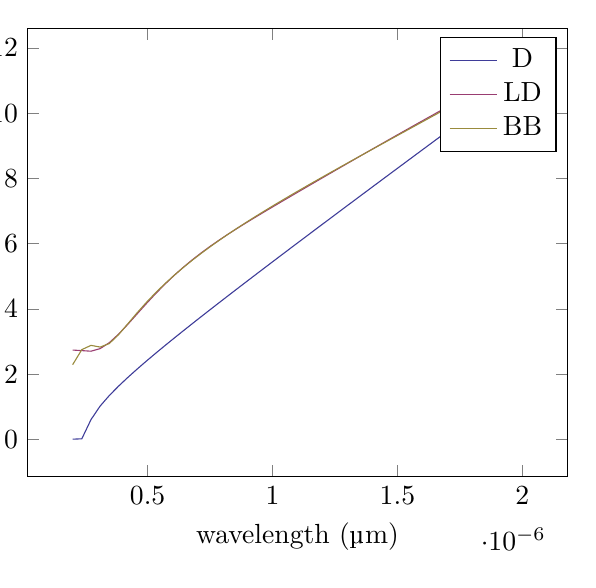
\begin{tikzpicture}[baseline,trim axis left]
			\begin{axis}[xlabel=wavelength (\si{\micro\meter}),ylabel=refractive index $n''$]
				\addplot[color=colora] coordinates {
						(2e-07, 0.005722070326258596)
						(2.3673469387755102e-07, 0.017087117472707893)
						(2.7346938775510205e-07, 0.6062709196238194)
						(3.1020408163265303e-07, 1.0227508619031003)
						(3.4693877551020406e-07, 1.3453567568284654)
						(3.836734693877551e-07, 1.6307481924056433)
						(4.2040816326530607e-07, 1.8957991509440735)
						(4.571428571428571e-07, 2.1480474973726613)
						(4.938775510204081e-07, 2.3915435244029113)
						(5.306122448979591e-07, 2.62871655193094)
						(5.673469387755102e-07, 2.861135587615447)
						(6.040816326530612e-07, 3.089869807332109)
						(6.408163265306121e-07, 3.3156781442134204)
						(6.775510204081632e-07, 3.5391169612176103)
						(7.142857142857142e-07, 3.760604933620124)
						(7.510204081632653e-07, 3.980464037279939)
						(7.877551020408163e-07, 4.198946461412275)
						(8.244897959183672e-07, 4.416252857770719)
						(8.612244897959183e-07, 4.632545057757891)
						(8.979591836734693e-07, 4.847955144982068)
						(9.346938775510204e-07, 5.062592061265287)
						(9.714285714285713e-07, 5.2765465037427415)
						(1.0081632653061223e-06, 5.489894613294939)
						(1.0448979591836734e-06, 5.702700792333309)
						(1.0816326530612245e-06, 5.915019885087764)
						(1.1183673469387754e-06, 6.126898884193696)
						(1.1551020408163265e-06, 6.3383782805749656)
						(1.1918367346938776e-06, 6.549493141452686)
						(1.2285714285714284e-06, 6.760273978831894)
						(1.2653061224489795e-06, 6.970747454871571)
						(1.3020408163265306e-06, 7.180936959073166)
						(1.3387755102040815e-06, 7.390863083866596)
						(1.3755102040816325e-06, 7.60054401901364)
						(1.4122448979591836e-06, 7.809995880659392)
						(1.4489795918367345e-06, 8.019232987408582)
						(1.4857142857142856e-06, 8.228268093179445)
						(1.5224489795918367e-06, 8.43711258457687)
						(1.5591836734693875e-06, 8.645776648972765)
						(1.5959183673469386e-06, 8.854269418271668)
						(1.6326530612244897e-06, 9.062599092390915)
						(1.6693877551020408e-06, 9.270773045735446)
						(1.7061224489795917e-06, 9.478797919352113)
						(1.7428571428571427e-06, 9.686679700972286)
						(1.7795918367346938e-06, 9.894423794769008)
						(1.8163265306122447e-06, 10.10203508234547)
						(1.8530612244897958e-06, 10.309517976220224)
						(1.8897959183673469e-06, 10.516876466869224)
						(1.9265306122448977e-06, 10.724114164216372)
						(1.963265306122449e-06, 10.931234334325408)
						(2e-06, 11.13823993193112)
					};
				\addlegendentry{D}
				\addplot[color=colorb] coordinates {
						(2e-07, 2.737818994015929)
						(2.3673469387755102e-07, 2.7206994578145096)
						(2.7346938775510205e-07, 2.702835287025359)
						(3.1020408163265303e-07, 2.7825533654999806)
						(3.4693877551020406e-07, 2.965785148981104)
						(3.836734693877551e-07, 3.223819926859244)
						(4.2040816326530607e-07, 3.523318564084796)
						(4.571428571428571e-07, 3.8382816762920595)
						(4.938775510204081e-07, 4.1519796066023655)
						(5.306122448979591e-07, 4.45482494159383)
						(5.673469387755102e-07, 4.741882009025515)
						(6.040816326530612e-07, 5.011120786926191)
						(6.408163265306121e-07, 5.262351367067391)
						(6.775510204081632e-07, 5.496565331723539)
						(7.142857142857142e-07, 5.715487688487498)
						(7.510204081632653e-07, 5.9212403636921405)
						(7.877551020408163e-07, 6.116079525091148)
						(8.244897959183672e-07, 6.30219701376335)
						(8.612244897959183e-07, 6.48158354883959)
						(8.979591836734693e-07, 6.655949171056373)
						(9.346938775510204e-07, 6.8266919352244715)
						(9.714285714285713e-07, 6.994902852823722)
						(1.0081632653061223e-06, 7.161394553712677)
						(1.0448979591836734e-06, 7.326742623461714)
						(1.0816326530612245e-06, 7.491331125941014)
						(1.1183673469387754e-06, 7.655396577385691)
						(1.1551020408163265e-06, 7.819067051131358)
						(1.1918367346938776e-06, 7.982394926143335)
						(1.2285714285714284e-06, 8.145383028403865)
						(1.2653061224489795e-06, 8.308004646561917)
						(1.3020408163265306e-06, 8.470218263723723)
						(1.3387755102040815e-06, 8.631977961283186)
						(1.3755102040816325e-06, 8.79324041855894)
						(1.4122448979591836e-06, 8.953969325217411)
						(1.4489795918367345e-06, 9.114137888356824)
						(1.4857142857142856e-06, 9.273729979954659)
						(1.5224489795918367e-06, 9.432740347256338)
						(1.5591836734693875e-06, 9.591174204407494)
						(1.5959183673469386e-06, 9.74904643917701)
						(1.6326530612244897e-06, 9.906380602443837)
						(1.6693877551020408e-06, 10.063207797612971)
						(1.7061224489795917e-06, 10.219565549419155)
						(1.7428571428571427e-06, 10.37549670398056)
						(1.7795918367346938e-06, 10.531048392151032)
						(1.8163265306122447e-06, 10.686271074273709)
						(1.8530612244897958e-06, 10.841217674840085)
						(1.8897959183673469e-06, 10.995942809129517)
						(1.9265306122448977e-06, 11.150502099751204)
						(1.963265306122449e-06, 11.304951578466587)
						(2e-06, 11.459347167243605)
					};
				\addlegendentry{LD}
				\addplot[color=colorc] coordinates {
						(2e-07, 2.2888414853724264)
						(2.3673469387755102e-07, 2.7516151284321357)
						(2.7346938775510205e-07, 2.881675675545906)
						(3.1020408163265303e-07, 2.8296976181318563)
						(3.4693877551020406e-07, 2.9384065658869662)
						(3.836734693877551e-07, 3.2087237381816878)
						(4.2040816326530607e-07, 3.5394541479507478)
						(4.571428571428571e-07, 3.8725804252393305)
						(4.938775510204081e-07, 4.188461500100237)
						(5.306122448979591e-07, 4.483124517962284)
						(5.673469387755102e-07, 4.757619611137122)
						(6.040816326530612e-07, 5.014305235383009)
						(6.408163265306121e-07, 5.255659047963557)
						(6.775510204081632e-07, 5.483928182263711)
						(7.142857142857142e-07, 5.701054374488825)
						(7.510204081632653e-07, 5.90868647830885)
						(7.877551020408163e-07, 6.108217156185248)
						(8.244897959183672e-07, 6.300822495644419)
						(8.612244897959183e-07, 6.487497863421518)
						(8.979591836734693e-07, 6.669088417968571)
						(9.346938775510204e-07, 6.84631443816062)
						(9.714285714285713e-07, 7.019792141910631)
						(1.0081632653061223e-06, 7.19005074653172)
						(1.0448979591836734e-06, 7.35754645469931)
						(1.0816326530612245e-06, 7.522673944267217)
						(1.1183673469387754e-06, 7.685775835843138)
						(1.1551020408163265e-06, 7.847150521146486)
						(1.1918367346938776e-06, 8.007058659971246)
						(1.2285714285714284e-06, 8.165728592780146)
						(1.2653061224489795e-06, 8.323360867322084)
						(1.3020408163265306e-06, 8.480132038922044)
						(1.3387755102040815e-06, 8.636197873256641)
						(1.3755102040816325e-06, 8.791696055860427)
						(1.4122448979591836e-06, 8.94674849299481)
						(1.4489795918367345e-06, 9.10146327281252)
						(1.4857142857142856e-06, 9.255936343148468)
						(1.5224489795918367e-06, 9.410252952120201)
						(1.5591836734693875e-06, 9.564488889524226)
						(1.5959183673469386e-06, 9.718711560372086)
						(1.6326530612244897e-06, 9.872980916510443)
						(1.6693877551020408e-06, 10.027350267866154)
						(1.7061224489795917e-06, 10.181866991255532)
						(1.7428571428571427e-06, 10.336573151741897)
						(1.7795918367346938e-06, 10.491506049093687)
						(1.8163265306122447e-06, 10.646698699888535)
						(1.8530612244897958e-06, 10.802180264147843)
						(1.8897959183673469e-06, 10.957976424007834)
						(1.9265306122448977e-06, 11.114109720786303)
						(1.963265306122449e-06, 11.270599855847152)
						(2e-06, 11.427463959864575)
					};
				\addlegendentry{BB}
			\end{axis}
		\end{tikzpicture}%
		\\
	\end{tabular}
	\caption{Complex permittivity $\epsilon = \epsilon' + \mi \epsilon''$ and refractive index $n = n' + \mi n''$ for Ni based on the Drude (D), Lorentz-Drude (LD), and Brendel-Bormann (BB) models.}
\end{figure}
\clearpage
\newpage
\subsection{W}
\begin{figure}[h!]
	\centering
	\begin{tabular}{l}
		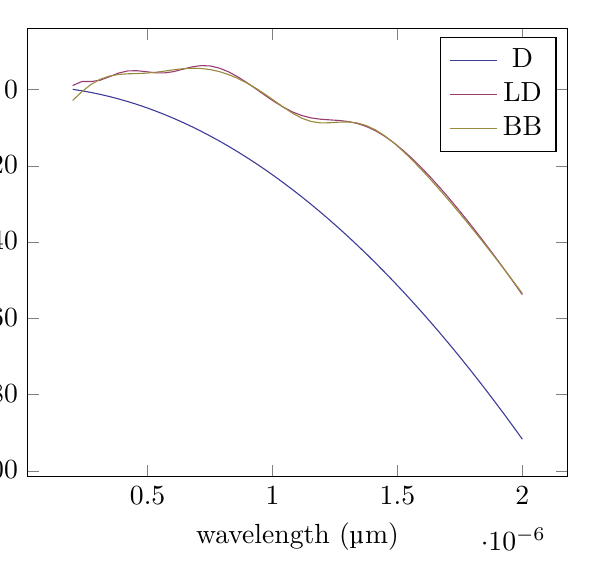
\begin{tikzpicture}[baseline,trim axis left]
			\begin{axis}[xlabel=wavelength (\si{\micro\meter}),ylabel=permittivity $\epsilon'$]
				\addplot[color=colora] coordinates {
						(2e-07, 0.06327705395381844)
						(2.3673469387755102e-07, -0.31237038905355186)
						(2.7346938775510205e-07, -0.7511701925195362)
						(3.1020408163265303e-07, -1.2531034331472237)
						(3.4693877551020406e-07, -1.8181484684781695)
						(3.836734693877551e-07, -2.446280939224605)
						(4.2040816326530607e-07, -3.137473771893731)
						(4.571428571428571e-07, -3.891697181703563)
						(4.938775510204081e-07, -4.708918675789729)
						(5.306122448979591e-07, -5.589103056702603)
						(5.673469387755102e-07, -6.532212426194051)
						(6.040816326530612e-07, -7.5382061892930246)
						(6.408163265306121e-07, -8.607041058669203)
						(6.775510204081632e-07, -9.738671059283813)
						(7.142857142857142e-07, -10.933047533326663)
						(7.510204081632653e-07, -12.190119145438432)
						(7.877551020408163e-07, -13.509831888217164)
						(8.244897959183672e-07, -14.892129088007861)
						(8.612244897959183e-07, -16.336951410974027)
						(8.979591836734693e-07, -17.844236869449908)
						(9.346938775510204e-07, -19.413920828572266)
						(9.714285714285713e-07, -21.045936013190225)
						(1.0081632653061223e-06, -22.74021251505198)
						(1.0448979591836734e-06, -24.496677800266713)
						(1.0816326530612245e-06, -26.315256717040533)
						(1.1183673469387754e-06, -28.19587150368456)
						(1.1551020408163265e-06, -30.13844179689396)
						(1.1918367346938776e-06, -32.142884640295875)
						(1.2285714285714284e-06, -34.20911449326484)
						(1.2653061224489795e-06, -36.33704324000399)
						(1.3020408163265306e-06, -38.526580198889945)
						(1.3387755102040815e-06, -40.77763213207984)
						(1.3755102040816325e-06, -43.09010325537853)
						(1.4122448979591836e-06, -45.46389524836395)
						(1.4489795918367345e-06, -47.89890726476867)
						(1.4857142857142856e-06, -50.39503594311583)
						(1.5224489795918367e-06, -52.95217541760695)
						(1.5591836734693875e-06, -55.570217329259876)
						(1.5959183673469386e-06, -58.2490508372945)
						(1.6326530612244897e-06, -60.98856263076416)
						(1.6693877551020408e-06, -63.78863694043018)
						(1.7061224489795917e-06, -66.64915555087782)
						(1.7428571428571427e-06, -69.56999781287053)
						(1.7795918367346938e-06, -72.55104065594085)
						(1.8163265306122447e-06, -75.59215860121488)
						(1.8530612244897958e-06, -78.69322377446859)
						(1.8897959183673469e-06, -81.8541059194126)
						(1.9265306122448977e-06, -85.07467241120362)
						(1.963265306122449e-06, -88.35478827017963)
						(2e-06, -91.69431617581616)
					};
				\addlegendentry{D}
				\addplot[color=colorb] coordinates {
						(2e-07, 1.055073447904749)
						(2.3673469387755102e-07, 2.1144594034196817)
						(2.7346938775510205e-07, 2.108291071687283)
						(3.1020408163265303e-07, 2.457193851158092)
						(3.4693877551020406e-07, 3.3615138122692385)
						(3.836734693877551e-07, 4.328301436912415)
						(4.2040816326530607e-07, 4.891984411038369)
						(4.571428571428571e-07, 4.9532224918105285)
						(4.938775510204081e-07, 4.6936961098895935)
						(5.306122448979591e-07, 4.408011098870274)
						(5.673469387755102e-07, 4.370230782875619)
						(6.040816326530612e-07, 4.708803285200496)
						(6.408163265306121e-07, 5.325593306718718)
						(6.775510204081632e-07, 5.948052716993068)
						(7.142857142857142e-07, 6.292778793587354)
						(7.510204081632653e-07, 6.1951980960405155)
						(7.877551020408163e-07, 5.626225444297848)
						(8.244897959183672e-07, 4.642142189396951)
						(8.612244897959183e-07, 3.33372065787103)
						(8.979591836734693e-07, 1.798738592397786)
						(9.346938775510204e-07, 0.13363547469375092)
						(9.714285714285713e-07, -1.5657746658970169)
						(1.0081632653061223e-06, -3.202286433551805)
						(1.0448979591836734e-06, -4.679190711288424)
						(1.0816326530612245e-06, -5.909462458277368)
						(1.1183673469387754e-06, -6.832904874898034)
						(1.1551020408163265e-06, -7.436905570731675)
						(1.1918367346938776e-06, -7.770754884548204)
						(1.2285714285714284e-06, -7.942369877899484)
						(1.2653061224489795e-06, -8.09417387774419)
						(1.3020408163265306e-06, -8.367764918871423)
						(1.3387755102040815e-06, -8.87369571291186)
						(1.3755102040816325e-06, -9.677431146961048)
						(1.4122448979591836e-06, -10.80159269135077)
						(1.4489795918367345e-06, -12.237451627426353)
						(1.4857142857142856e-06, -13.958187304456565)
						(1.5224489795918367e-06, -15.929569803767656)
						(1.5591836734693875e-06, -18.11686889149115)
						(1.5959183673469386e-06, -20.488521079127082)
						(1.6326530612244897e-06, -23.017595311391325)
						(1.6693877551020408e-06, -25.681990106935174)
						(1.7061224489795917e-06, -28.464010141447858)
						(1.7428571428571427e-06, -31.349709233989728)
						(1.7795918367346938e-06, -34.32820391895824)
						(1.8163265306122447e-06, -37.39105087093262)
						(1.8530612244897958e-06, -40.53172077036726)
						(1.8897959183673469e-06, -43.74517118182607)
						(1.9265306122448977e-06, -47.027508092485405)
						(1.963265306122449e-06, -50.37572164406523)
						(2e-06, -53.78748162425215)
					};
				\addlegendentry{LD}
				\addplot[color=colorc] coordinates {
						(2e-07, -2.845871380174961)
						(2.3673469387755102e-07, -0.5761425157239749)
						(2.7346938775510205e-07, 1.3480459172618398)
						(3.1020408163265303e-07, 2.708058012198072)
						(3.4693877551020406e-07, 3.542616653225247)
						(3.836734693877551e-07, 3.9692178618264893)
						(4.2040816326530607e-07, 4.1353959435615675)
						(4.571428571428571e-07, 4.201716671714016)
						(4.938775510204081e-07, 4.307596661715995)
						(5.306122448979591e-07, 4.5258523153180255)
						(5.673469387755102e-07, 4.844640028465327)
						(6.040816326530612e-07, 5.19079717750617)
						(6.408163265306121e-07, 5.471188083537953)
						(6.775510204081632e-07, 5.604942647575527)
						(7.142857142857142e-07, 5.537277221241093)
						(7.510204081632653e-07, 5.239329044107162)
						(7.877551020408163e-07, 4.701693099922851)
						(8.244897959183672e-07, 3.9271505505553037)
						(8.612244897959183e-07, 2.9252440407878026)
						(8.979591836734693e-07, 1.7097105787080764)
						(9.346938775510204e-07, 0.2994386118771004)
						(9.714285714285713e-07, -1.2758452330187353)
						(1.0081632653061223e-06, -2.9635900690126356)
						(1.0448979591836734e-06, -4.671358164805799)
						(1.0816326530612245e-06, -6.2557816481885204)
						(1.1183673469387754e-06, -7.5404942112483475)
						(1.1551020408163265e-06, -8.377794276191754)
						(1.1918367346938776e-06, -8.729258013198567)
						(1.2285714285714284e-06, -8.707257144689542)
						(1.2653061224489795e-06, -8.540741261452588)
						(1.3020408163265306e-06, -8.48790606821899)
						(1.3387755102040815e-06, -8.752392316636723)
						(1.3755102040816325e-06, -9.442902826061232)
						(1.4122448979591836e-06, -10.57843654803824)
						(1.4489795918367345e-06, -12.118154289206885)
						(1.4857142857142856e-06, -13.994036462617693)
						(1.5224489795918367e-06, -16.134622055173367)
						(1.5591836734693875e-06, -18.47770483547442)
						(1.5959183673469386e-06, -20.974683608647226)
						(1.6326530612244897e-06, -23.590184927035104)
						(1.6693877551020408e-06, -26.299717372217735)
						(1.7061224489795917e-06, -29.086948199422515)
						(1.7428571428571427e-06, -31.94131495651944)
						(1.7795918367346938e-06, -34.85617988347221)
						(1.8163265306122447e-06, -37.82750201401513)
						(1.8530612244897958e-06, -40.852922988688746)
						(1.8897959183673469e-06, -43.93115533766293)
						(1.9265306122448977e-06, -47.06158081426129)
						(1.963265306122449e-06, -50.24399008139969)
						(2e-06, -53.47841567801875)
					};
				\addlegendentry{BB}
			\end{axis}
		\end{tikzpicture}%
		\\
		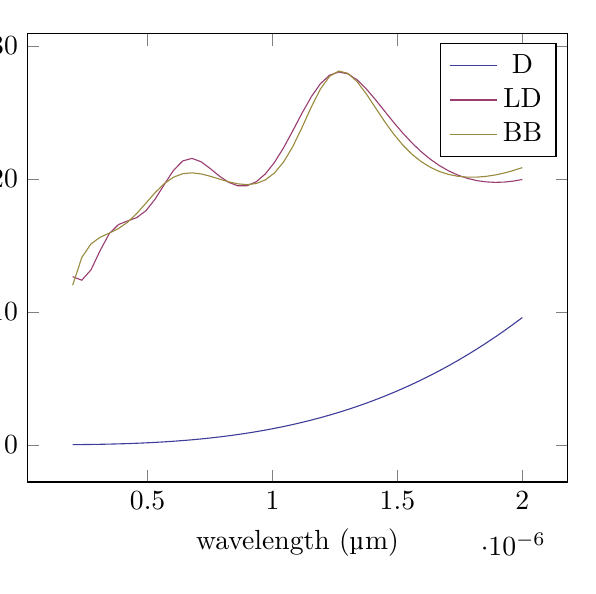
\begin{tikzpicture}[baseline,trim axis left]
			\begin{axis}[xlabel=wavelength (\si{\micro\meter}),ylabel=permittivity $\epsilon''$]
				\addplot[color=colora] coordinates {
						(2e-07, 0.0096706305004271)
						(2.3673469387755102e-07, 0.01603732636811167)
						(2.7346938775510205e-07, 0.024720127704277003)
						(3.1020408163265303e-07, 0.03607798491150466)
						(3.4693877551020406e-07, 0.0504696561640789)
						(3.836734693877551e-07, 0.06825368167345434)
						(4.2040816326530607e-07, 0.08978835798659662)
						(4.571428571428571e-07, 0.11543171232106025)
						(4.938775510204081e-07, 0.14554147694065891)
						(5.306122448979591e-07, 0.18047506357557258)
						(5.673469387755102e-07, 0.2205895378907245)
						(6.040816326530612e-07, 0.2662415940062484)
						(6.408163265306121e-07, 0.3177875290738534)
						(6.775510204081632e-07, 0.37558321791287896)
						(7.142857142857142e-07, 0.43998408770981867)
						(7.510204081632653e-07, 0.5113450927850702)
						(7.877551020408163e-07, 0.5900206894306605)
						(8.244897959183672e-07, 0.6763648108226682)
						(8.612244897959183e-07, 0.7707308420120498)
						(8.979591836734693e-07, 0.8734715949975541)
						(9.346938775510204e-07, 0.9849392838843997)
						(9.714285714285713e-07, 1.1054855001323431)
						(1.0081632653061223e-06, 1.2354611878967736)
						(1.0448979591836734e-06, 1.3752166194664168)
						(1.0816326530612245e-06, 1.525101370801237)
						(1.1183673469387754e-06, 1.6854642971740592)
						(1.1551020408163265e-06, 1.8566535089194667)
						(1.1918367346938776e-06, 2.0390163472934235)
						(1.2285714285714284e-06, 2.2328993604471257)
						(1.2653061224489795e-06, 2.438648279518497)
						(1.3020408163265306e-06, 2.656607994844735)
						(1.3387755102040815e-06, 2.8871225322992915)
						(1.3755102040816325e-06, 3.130535029756628)
						(1.4122448979591836e-06, 3.3871877136880446)
						(1.4489795918367345e-06, 3.657421875891891)
						(1.4857142857142856e-06, 3.941577850361383)
						(1.5224489795918367e-06, 4.239994990293231)
						(1.5591836734693875e-06, 4.553011645240267)
						(1.5959183673469386e-06, 4.880965138411216)
						(1.6326530612244897e-06, 5.224191744120703)
						(1.6693877551020408e-06, 5.583026665392545)
						(1.7061224489795917e-06, 5.957804011719411)
						(1.7428571428571427e-06, 6.348856776981768)
						(1.7795918367346938e-06, 6.7565168175291195)
						(1.8163265306122447e-06, 7.181114830426394)
						(1.8530612244897958e-06, 7.622980331868435)
						(1.8897959183673469e-06, 8.082441635765289)
						(1.9265306122448977e-06, 8.559825832501216)
						(1.963265306122449e-06, 9.055458767870096)
						(2e-06, 9.569665022189886)
					};
				\addlegendentry{D}
				\addplot[color=colorb] coordinates {
						(2e-07, 12.642227935346472)
						(2.3673469387755102e-07, 12.375837387494943)
						(2.7346938775510205e-07, 13.155030560393897)
						(3.1020408163265303e-07, 14.611614638812197)
						(3.4693877551020406e-07, 15.883406893916252)
						(3.836734693877551e-07, 16.56290640140384)
						(4.2040816326530607e-07, 16.833823176067924)
						(4.571428571428571e-07, 17.087344390701105)
						(4.938775510204081e-07, 17.60955728968222)
						(5.306122448979591e-07, 18.484799118241924)
						(5.673469387755102e-07, 19.58978163034749)
						(6.040816326530612e-07, 20.64327959068015)
						(6.408163265306121e-07, 21.343281350199344)
						(6.775510204081632e-07, 21.53642383363654)
						(7.142857142857142e-07, 21.28062841319536)
						(7.510204081632653e-07, 20.765626716745903)
						(7.877551020408163e-07, 20.197151417791392)
						(8.244897959183672e-07, 19.73315238633505)
						(8.612244897959183e-07, 19.47448988191558)
						(8.979591836734693e-07, 19.47855776506093)
						(9.346938775510204e-07, 19.77365809328998)
						(9.714285714285713e-07, 20.366278537166334)
						(1.0081632653061223e-06, 21.240726176565566)
						(1.0448979591836734e-06, 22.35341042163837)
						(1.0816326530612245e-06, 23.626008553372486)
						(1.1183673469387754e-06, 24.943819933026994)
						(1.1551020408163265e-06, 26.166127835786803)
						(1.1918367346938776e-06, 27.15126057356843)
						(1.2285714285714284e-06, 27.78982518038989)
						(1.2653061224489795e-06, 28.03135140017157)
						(1.3020408163265306e-06, 27.89107192866726)
						(1.3387755102040815e-06, 27.435310967532192)
						(1.3755102040816325e-06, 26.755719096933667)
						(1.4122448979591836e-06, 25.94515301887607)
						(1.4489795918367345e-06, 25.082454379935424)
						(1.4857142857142856e-06, 24.22664148882637)
						(1.5224489795918367e-06, 23.417481001914783)
						(1.5591836734693875e-06, 22.679045591960147)
						(1.5959183673469386e-06, 22.023934529919803)
						(1.6326530612244897e-06, 21.457004566198528)
						(1.6693877551020408e-06, 20.978239913012438)
						(1.7061224489795917e-06, 20.584782031751658)
						(1.7428571428571427e-06, 20.27228295277655)
						(1.7795918367346938e-06, 20.035765206143587)
						(1.8163265306122447e-06, 19.870143113806368)
						(1.8530612244897958e-06, 19.770521293837177)
						(1.8897959183673469e-06, 19.73235144256165)
						(1.9265306122448977e-06, 19.75150174826061)
						(1.963265306122449e-06, 19.824274304602017)
						(2e-06, 19.947393001361196)
					};
				\addlegendentry{LD}
				\addplot[color=colorc] coordinates {
						(2e-07, 11.997206664290111)
						(2.3673469387755102e-07, 14.083538837526136)
						(2.7346938775510205e-07, 15.109801315036727)
						(3.1020408163265303e-07, 15.605864733581313)
						(3.4693877551020406e-07, 15.919608131228832)
						(3.836734693877551e-07, 16.25973219378264)
						(4.2040816326530607e-07, 16.742543979624532)
						(4.571428571428571e-07, 17.401019288724342)
						(4.938775510204081e-07, 18.181852415426004)
						(5.306122448979591e-07, 18.970275734544586)
						(5.673469387755102e-07, 19.644519414166723)
						(6.040816326530612e-07, 20.12386009012018)
						(6.408163265306121e-07, 20.384709165266806)
						(6.775510204081632e-07, 20.449531982808885)
						(7.142857142857142e-07, 20.36620737533888)
						(7.510204081632653e-07, 20.190572756804787)
						(7.877551020408163e-07, 19.976358479048127)
						(8.244897959183672e-07, 19.771687194633476)
						(8.612244897959183e-07, 19.619919203898757)
						(8.979591836734693e-07, 19.562965589239038)
						(9.346938775510204e-07, 19.64576581575466)
						(9.714285714285713e-07, 19.92041755676693)
						(1.0081632653061223e-06, 20.446419034027926)
						(1.0448979591836734e-06, 21.279472622806892)
						(1.0816326530612245e-06, 22.440270382625293)
						(1.1183673469387754e-06, 23.86803674825649)
						(1.1551020408163265e-06, 25.390933234117128)
						(1.1918367346938776e-06, 26.75418131130469)
						(1.2285714285714284e-06, 27.707785584878874)
						(1.2653061224489795e-06, 28.101653939802244)
						(1.3020408163265306e-06, 27.928470322843822)
						(1.3387755102040815e-06, 27.299140793780026)
						(1.3755102040816325e-06, 26.381022860933598)
						(1.4122448979591836e-06, 25.33888825639062)
						(1.4489795918367345e-06, 24.30042873194124)
						(1.4857142857142856e-06, 23.34701375685593)
						(1.5224489795918367e-06, 22.520041333219716)
						(1.5591836734693875e-06, 21.832881453668342)
						(1.5959183673469386e-06, 21.28225687704862)
						(1.6326530612244897e-06, 20.856669514937458)
						(1.6693877551020408e-06, 20.541715064435945)
						(1.7061224489795917e-06, 20.32300668064987)
						(1.7428571428571427e-06, 20.187544608902883)
						(1.7795918367346938e-06, 20.124191287825685)
						(1.8163265306122447e-06, 20.123687297614364)
						(1.8530612244897958e-06, 20.17846429691094)
						(1.8897959183673469e-06, 20.282392007199228)
						(1.9265306122448977e-06, 20.43052552868326)
						(1.963265306122449e-06, 20.61888059219194)
						(2e-06, 20.84424480995272)
					};
				\addlegendentry{BB}
			\end{axis}
		\end{tikzpicture}%
		\\
		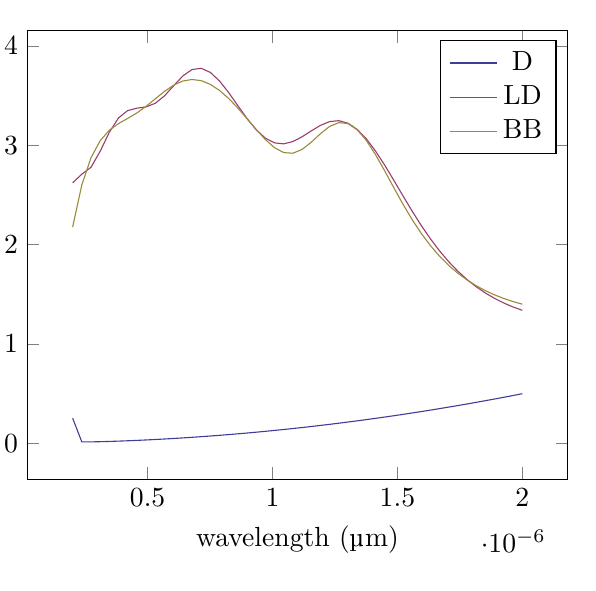
\begin{tikzpicture}[baseline,trim axis left]
			\begin{axis}[xlabel=wavelength (\si{\micro\meter}),ylabel=refractive index $n'$]
				\addplot[color=colora] coordinates {
						(2e-07, 0.2522784409985043)
						(2.3673469387755102e-07, 0.014342474641386337)
						(2.7346938775510205e-07, 0.014259121611277306)
						(3.1020408163265303e-07, 0.016112904451971475)
						(3.4693877551020406e-07, 0.018713019036329152)
						(3.836734693877551e-07, 0.021817283407291603)
						(4.2040816326530607e-07, 0.02534285477761303)
						(4.571428571428571e-07, 0.029253502950255358)
						(4.938775510204081e-07, 0.033530833293687154)
						(5.306122448979591e-07, 0.03816449916461437)
						(5.673469387755102e-07, 0.0431482200013977)
						(6.040816326530612e-07, 0.04847794656583351)
						(6.408163265306121e-07, 0.05415093379353621)
						(6.775510204081632e-07, 0.060165237573972845)
						(7.142857142857142e-07, 0.06651942556546332)
						(7.510204081632653e-07, 0.07321240304775763)
						(7.877551020408163e-07, 0.0802433038704097)
						(8.244897959183672e-07, 0.08761141986141924)
						(8.612244897959183e-07, 0.09531615381028921)
						(8.979591836734693e-07, 0.10335698736669671)
						(9.346938775510204e-07, 0.11173345864105484)
						(9.714285714285713e-07, 0.1204451462710812)
						(1.0081632653061223e-06, 0.12949165789224296)
						(1.0448979591836734e-06, 0.13887262166578362)
						(1.0816326530612245e-06, 0.14858767996705266)
						(1.1183673469387754e-06, 0.1586364846244913)
						(1.1551020408163265e-06, 0.1690186932875135)
						(1.1918367346938776e-06, 0.17973396662722282)
						(1.2285714285714284e-06, 0.19078196615904375)
						(1.2653061224489795e-06, 0.20216235253473133)
						(1.3020408163265306e-06, 0.21387478419267458)
						(1.3387755102040815e-06, 0.22591891628380142)
						(1.3755102040816325e-06, 0.23829439981202227)
						(1.4122448979591836e-06, 0.251000880942409)
						(1.4489795918367345e-06, 0.26403800044211145)
						(1.4857142857142856e-06, 0.2774053932267863)
						(1.5224489795918367e-06, 0.2911026879915103)
						(1.5591836734693875e-06, 0.3051295069099435)
						(1.5959183673469386e-06, 0.31948546538883393)
						(1.6326530612244897e-06, 0.3341701718676653)
						(1.6693877551020408e-06, 0.3491832276555263)
						(1.7061224489795917e-06, 0.36452422679856095)
						(1.7428571428571427e-06, 0.3801927559729724)
						(1.7795918367346938e-06, 0.3961883943991756)
						(1.8163265306122447e-06, 0.41251071377392445)
						(1.8530612244897958e-06, 0.42915927821739597)
						(1.8897959183673469e-06, 0.44613364423305224)
						(1.9265306122448977e-06, 0.46343336067834834)
						(1.963265306122449e-06, 0.48105796874477535)
						(2e-06, 0.4990070019458287)
					};
				\addlegendentry{D}
				\addplot[color=colorb] coordinates {
						(2e-07, 2.6211878268238573)
						(2.3673469387755102e-07, 2.708286288356964)
						(2.7346938775510205e-07, 2.7776962728804224)
						(3.1020408163265303e-07, 2.9388754406982796)
						(3.4693877551020406e-07, 3.1302343734749085)
						(3.836734693877551e-07, 3.2747072669280444)
						(4.2040816326530607e-07, 3.3482994713204164)
						(4.571428571428571e-07, 3.372239584874935)
						(4.938775510204081e-07, 3.3851186047959425)
						(5.306122448979591e-07, 3.4213393275197848)
						(5.673469387755102e-07, 3.4958235870642547)
						(6.040816326530612e-07, 3.597382399016358)
						(6.408163265306121e-07, 3.6961646321520187)
						(6.775510204081632e-07, 3.7610348991586786)
						(7.142857142857142e-07, 3.7738782077909065)
						(7.510204081632653e-07, 3.732644066121044)
						(7.877551020408163e-07, 3.6463936208510823)
						(8.244897959183672e-07, 3.5294450472361665)
						(8.612244897959183e-07, 3.397903030199906)
						(8.979591836734693e-07, 3.2680400779455803)
						(9.346938775510204e-07, 3.1549758425626235)
						(9.714285714285713e-07, 3.070879691193014)
						(1.0081632653061223e-06, 3.0231171348016983)
						(1.0448979591836734e-06, 3.013196942328032)
						(1.0816326530612245e-06, 3.0368065371727266)
						(1.1183673469387754e-06, 3.0846282278518173)
						(1.1551020408163265e-06, 3.143688444153952)
						(1.1918367346938776e-06, 3.199267555749598)
						(1.2285714285714284e-06, 3.237294351652728)
						(1.2653061224489795e-06, 3.2467212237547063)
						(1.3020408163265306e-06, 3.2211408271643505)
						(1.3387755102040815e-06, 3.159191681588256)
						(1.3755102040816325e-06, 3.0638745491540553)
						(1.4122448979591836e-06, 2.9412785698552404)
						(1.4489795918367345e-06, 2.7992012219609466)
						(1.4857142857142856e-06, 2.645921829914358)
						(1.5224489795918367e-06, 2.489209008464127)
						(1.5591836734693875e-06, 2.335595857091647)
						(1.5959183673469386e-06, 2.1899685157506195)
						(1.6326530612244897e-06, 2.055486632737738)
						(1.6693877551020408e-06, 1.933778491024032)
						(1.7061224489795917e-06, 1.8252909513227435)
						(1.7428571428571427e-06, 1.7296699471003465)
						(1.7795918367346938e-06, 1.6460888531627975)
						(1.8163265306122447e-06, 1.5734922546181043)
						(1.8530612244897958e-06, 1.5107572055363128)
						(1.8897959183673469e-06, 1.4567893393718665)
						(1.9265306122448977e-06, 1.4105736300946208)
						(1.963265306122449e-06, 1.3711963002684802)
						(2e-06, 1.337849727072408)
					};
				\addlegendentry{LD}
				\addplot[color=colorc] coordinates {
						(2e-07, 2.177642345349921)
						(2.3673469387755102e-07, 2.59992077596018)
						(2.7346938775510205e-07, 2.8738356005828214)
						(3.1020408163265303e-07, 3.045253875952932)
						(3.4693877551020406e-07, 3.1505264858034265)
						(3.836734693877551e-07, 3.21763961824277)
						(4.2040816326530607e-07, 3.2696405867941176)
						(4.571428571428571e-07, 3.3243669344861)
						(4.938775510204081e-07, 3.3906308491566293)
						(5.306122448979591e-07, 3.466160466708472)
						(5.673469387755102e-07, 3.541025545481527)
						(6.040816326530612e-07, 3.6037023198581886)
						(6.408163265306121e-07, 3.645363811892077)
						(6.775510204081632e-07, 3.661194217354306)
						(7.142857142857142e-07, 3.649850529171663)
						(7.510204081632653e-07, 3.6123825016307762)
						(7.877551020408163e-07, 3.5513304621473396)
						(8.244897959183672e-07, 3.470236314415716)
						(8.612244897959183e-07, 3.37357637893633)
						(8.979591836734693e-07, 3.2670509911375354)
						(9.346938775510204e-07, 3.1581233589255073)
						(9.714285714285713e-07, 3.056582046341781)
						(1.0081632653061223e-06, 2.9745999913184)
						(1.0448979591836734e-06, 2.925305079301644)
						(1.0816326530612245e-06, 2.9189169487720577)
						(1.1183673469387754e-06, 2.9572226334599687)
						(1.1551020408163265e-06, 3.029816431513543)
						(1.1918367346938776e-06, 3.115524892232227)
						(1.2285714285714284e-06, 3.1887664936439712)
						(1.2653061224489795e-06, 3.227236844810585)
						(1.3020408163265306e-06, 3.2172882010124266)
						(1.3387755102040815e-06, 3.1555894616064712)
						(1.3755102040816325e-06, 3.047721365077183)
						(1.4122448979591836e-06, 2.9051628579319875)
						(1.4489795918367345e-06, 2.7419179795275452)
						(1.4857142857142856e-06, 2.571549896888956)
						(1.5224489795918367e-06, 2.4050755167008493)
						(1.5591836734693875e-06, 2.249971961660957)
						(1.5959183673469386e-06, 2.110246082374889)
						(1.6326530612244897e-06, 1.9871925139311999)
						(1.6693877551020408e-06, 1.880357101383341)
						(1.7061224489795917e-06, 1.788365293380221)
						(1.7428571428571427e-06, 1.7094913860339163)
						(1.7795918367346938e-06, 1.641988583763323)
						(1.8163265306122447e-06, 1.5842505721591595)
						(1.8530612244897958e-06, 1.5348722509000616)
						(1.8897959183673469e-06, 1.4926573634419678)
						(1.9265306122448977e-06, 1.4566018057774834)
						(1.963265306122449e-06, 1.4258682042112671)
						(2e-06, 1.3997594316372195)
					};
				\addlegendentry{BB}
			\end{axis}
		\end{tikzpicture}%
		\\
		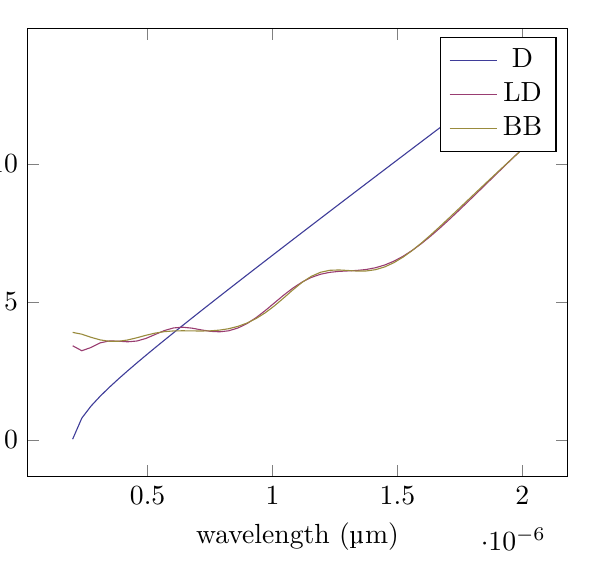
\begin{tikzpicture}[baseline,trim axis left]
			\begin{axis}[xlabel=wavelength (\si{\micro\meter}),ylabel=refractive index $n''$]
				\addplot[color=colora] coordinates {
						(2e-07, 0.027105639222029174)
						(2.3673469387755102e-07, 0.7906656633905265)
						(2.7346938775510205e-07, 1.2258658287664774)
						(3.1020408163265303e-07, 1.5832643865363119)
						(3.4693877551020406e-07, 1.9070913169324764)
						(3.836734693877551e-07, 2.212128808672713)
						(4.2040816326530607e-07, 2.505240919425519)
						(4.571428571428571e-07, 2.7901802626849843)
						(4.938775510204081e-07, 3.0692158583491964)
						(5.306122448979591e-07, 3.3438180529745005)
						(5.673469387755102e-07, 3.614989403880277)
						(6.040816326530612e-07, 3.8834408198390933)
						(6.408163265306121e-07, 4.149692369875125)
						(6.775510204081632e-07, 4.414134323986108)
						(7.142857142857142e-07, 4.6770658253448225)
						(7.510204081632653e-07, 4.938720320366088)
						(7.877551020408163e-07, 5.199282811317961)
						(8.244897959183672e-07, 5.458901876549531)
						(8.612244897959183e-07, 5.717698239702969)
						(8.979591836734693e-07, 5.975771002353993)
						(9.346938775510204e-07, 6.233202257965348)
						(9.714285714285713e-07, 6.490060561574212)
						(1.0081632653061223e-06, 6.746403575908524)
						(1.0448979591836734e-06, 7.002280115121794)
						(1.0816326530612245e-06, 7.257731741484873)
						(1.1183673469387754e-06, 7.51279402591853)
						(1.1551020408163265e-06, 7.767497552696696)
						(1.1918367346938776e-06, 8.021868727304808)
						(1.2285714285714284e-06, 8.275930431302132)
						(1.2653061224489795e-06, 8.52970255715712)
						(1.3020408163265306e-06, 8.783202448105522)
						(1.3387755102040815e-06, 9.036445262249385)
						(1.3755102040816325e-06, 9.289444275774553)
						(1.4122448979591836e-06, 9.542211136900903)
						(1.4489795918367345e-06, 9.794756079703683)
						(1.4857142857142856e-06, 10.047088105048859)
						(1.5224489795918367e-06, 10.299215134422898)
						(1.5591836734693875e-06, 10.55114414130022)
						(1.5959183673469386e-06, 10.802881263800803)
						(1.6326530612244897e-06, 11.054431901688138)
						(1.6693877551020408e-06, 11.30580080020041)
						(1.7061224489795917e-06, 11.556992122762818)
						(1.7428571428571427e-06, 11.808009514271644)
						(1.7795918367346938e-06, 12.058856156352265)
						(1.8163265306122447e-06, 12.309534815759134)
						(1.8530612244897958e-06, 12.56004788689507)
						(1.8897959183673469e-06, 12.810397429270434)
						(1.9265306122448977e-06, 13.06058520059444)
						(1.963265306122449e-06, 13.310612686084173)
						(2e-06, 13.560481124488698)
					};
				\addlegendentry{D}
				\addplot[color=colorb] coordinates {
						(2e-07, 3.410440492248715)
						(2.3673469387755102e-07, 3.2312088190900505)
						(2.7346938775510205e-07, 3.3488223341009022)
						(3.1020408163265303e-07, 3.5156208569131615)
						(3.4693877551020406e-07, 3.5879948217952085)
						(3.836734693877551e-07, 3.5764245405597275)
						(4.2040816326530607e-07, 3.555031628159225)
						(4.571428571428571e-07, 3.582953342143028)
						(4.938775510204081e-07, 3.678405050737625)
						(5.306122448979591e-07, 3.820353830514461)
						(5.673469387755102e-07, 3.962461802717896)
						(6.040816326530612e-07, 4.057673431796156)
						(6.408163265306121e-07, 4.083145767971737)
						(6.775510204081632e-07, 4.049032179594642)
						(7.142857142857142e-07, 3.987324399557114)
						(7.510204081632653e-07, 3.9338107804794387)
						(7.877551020408163e-07, 3.916621246402471)
						(8.244897959183672e-07, 3.9534390477312176)
						(8.612244897959183e-07, 4.052659458866653)
						(8.979591836734693e-07, 4.2145812030759995)
						(9.346938775510204e-07, 4.431757460073823)
						(9.714285714285713e-07, 4.689579244170786)
						(1.0081632653061223e-06, 4.968203627928999)
						(1.0448979591836734e-06, 5.2456737459631295)
						(1.0816326530612245e-06, 5.501210121871801)
						(1.1183673469387754e-06, 5.718012972870606)
						(1.1551020408163265e-06, 5.885521659910661)
						(1.1918367346938776e-06, 6.001011211091046)
						(1.2285714285714284e-06, 6.069999109908031)
						(1.2653061224489795e-06, 6.104977081451404)
						(1.3020408163265306e-06, 6.122664966711222)
						(1.3387755102040815e-06, 6.140714582836154)
						(1.3755102040816325e-06, 6.174910266540723)
						(1.4122448979591836e-06, 6.2374213128247895)
						(1.4489795918367345e-06, 6.336083823380813)
						(1.4857142857142856e-06, 6.474425014543595)
						(1.5224489795918367e-06, 6.65217728139992)
						(1.5591836734693875e-06, 6.866130919106453)
						(1.5959183673469386e-06, 7.1111860022229845)
						(1.6326530612244897e-06, 7.381411871553415)
						(1.6693877551020408e-06, 7.670917723360401)
						(1.7061224489795917e-06, 7.9744212578002855)
						(1.7428571428571427e-06, 8.287516800573238)
						(1.7795918367346938e-06, 8.606719750458366)
						(1.8163265306122447e-06, 8.929381697102636)
						(1.8530612244897958e-06, 9.25355154569824)
						(1.8897959183673469e-06, 9.57782922808019)
						(1.9265306122448977e-06, 9.90123487837792)
						(1.963265306122449e-06, 10.223101382450944)
						(2e-06, 10.542990421742767)
					};
				\addlegendentry{LD}
				\addplot[color=colorc] coordinates {
						(2e-07, 3.895637961730034)
						(2.3673469387755102e-07, 3.830334334491798)
						(2.7346938775510205e-07, 3.7177641511842534)
						(3.1020408163265303e-07, 3.623675801395121)
						(3.4693877551020406e-07, 3.5730100712210824)
						(3.836734693877551e-07, 3.573230149615049)
						(4.2040816326530607e-07, 3.6208158260949475)
						(4.571428571428571e-07, 3.701269739802949)
						(4.938775510204081e-07, 3.7917755454500766)
						(5.306122448979591e-07, 3.8699912314253804)
						(5.673469387755102e-07, 3.9228106977745996)
						(6.040816326530612e-07, 3.9486385584515387)
						(6.408163265306121e-07, 3.954109062105997)
						(6.775510204081632e-07, 3.9495317316393557)
						(7.142857142857142e-07, 3.945663864054712)
						(7.510204081632653e-07, 3.952209076954575)
						(7.877551020408163e-07, 3.977500459196149)
						(8.244897959183672e-07, 4.028744103894978)
						(8.612244897959183e-07, 4.112365145200353)
						(8.979591836734693e-07, 4.234126025518059)
						(9.346938775510204e-07, 4.398705386432201)
						(9.714285714285713e-07, 4.608370436290392)
						(1.0081632653061223e-06, 4.86041874273484)
						(1.0448979591836734e-06, 5.14368894312123)
						(1.0816326530612245e-06, 5.436148968160696)
						(1.1183673469387754e-06, 5.7071288604860255)
						(1.1551020408163265e-06, 5.925804904797527)
						(1.1918367346938776e-06, 6.072191263014893)
						(1.2285714285714284e-06, 6.144182434738736)
						(1.2653061224489795e-06, 6.157239464882874)
						(1.3020408163265306e-06, 6.138216261519753)
						(1.3387755102040815e-06, 6.117211320011521)
						(1.3755102040816325e-06, 6.12070393749104)
						(1.4122448979591836e-06, 6.1673994161471)
						(1.4489795918367345e-06, 6.2667804326724745)
						(1.4857142857142856e-06, 6.419798335587699)
						(1.5224489795918367e-06, 6.621028665729703)
						(1.5591836734693875e-06, 6.861498183885918)
						(1.5959183673469386e-06, 7.131314344049882)
						(1.6326530612244897e-06, 7.421471419396467)
						(1.6693877551020408e-06, 7.7246954892656445)
						(1.7061224489795917e-06, 8.03557074786719)
						(1.7428571428571427e-06, 8.350290504580496)
						(1.7795918367346938e-06, 8.666291755148945)
						(1.8163265306122447e-06, 8.98190980687312)
						(1.8530612244897958e-06, 9.296101958915013)
						(1.8897959183673469e-06, 9.608244516278763)
						(1.9265306122448977e-06, 9.917990687115562)
						(1.963265306122449e-06, 10.225173858392859)
						(2e-06, 10.529742840589803)
					};
				\addlegendentry{BB}
			\end{axis}
		\end{tikzpicture}%
		\\
	\end{tabular}
	\caption{Complex permittivity $\epsilon = \epsilon' + \mi \epsilon''$ and refractive index $n = n' + \mi n''$ for W based on the Drude (D), Lorentz-Drude (LD), and Brendel-Bormann (BB) models.}
\end{figure}
\clearpage
\newpage
\subsection{Ti}
\begin{figure}[h!]
	\centering
	\begin{tabular}{l}
		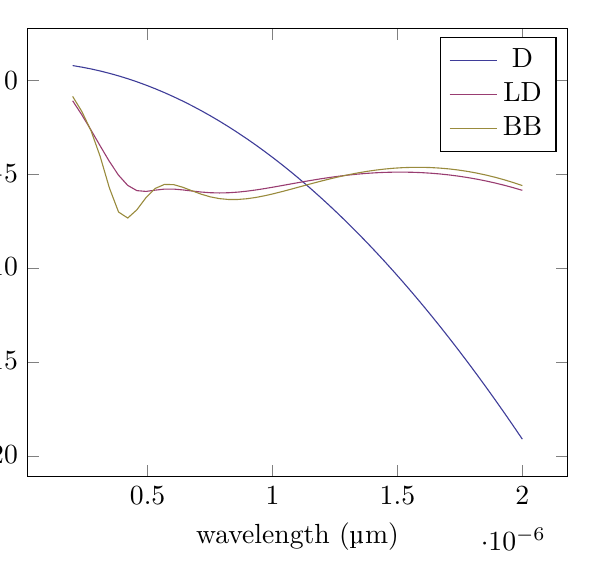
\begin{tikzpicture}[baseline,trim axis left]
			\begin{axis}[xlabel=wavelength (\si{\micro\meter}),ylabel=permittivity $\epsilon'$]
				\addplot[color=colora] coordinates {
						(2e-07, 0.7953705647067915)
						(2.3673469387755102e-07, 0.7133173157797221)
						(2.7346938775510205e-07, 0.6174752970963419)
						(3.1020408163265303e-07, 0.507851291408017)
						(3.4693877551020406e-07, 0.38445305477412817)
						(3.836734693877551e-07, 0.24728931519090924)
						(4.2040816326530607e-07, 0.0963697710491267)
						(4.571428571428571e-07, -0.0682949105788897)
						(4.938775510204081e-07, -0.24669309582229992)
						(5.306122448979591e-07, -0.43881218606427597)
						(5.673469387755102e-07, -0.6446386201633116)
						(6.040816326530612e-07, -0.8641578768425917)
						(6.408163265306121e-07, -1.0973544772466366)
						(6.775510204081632e-07, -1.3442119876643903)
						(7.142857142857142e-07, -1.6047130224178412)
						(7.510204081632653e-07, -1.8788392469152506)
						(7.877551020408163e-07, -2.1665713808679796)
						(8.244897959183672e-07, -2.4678892016698653)
						(8.612244897959183e-07, -2.7827715479380464)
						(8.979591836734693e-07, -3.1111963232140765)
						(9.346938775510204e-07, -3.4531404998241397)
						(9.714285714285713e-07, -3.808580122897097)
						(1.0081632653061223e-06, -4.177490314539072)
						(1.0448979591836734e-06, -4.559845278163208)
						(1.0816326530612245e-06, -4.955618302973234)
						(1.1183673469387754e-06, -5.364781768599334)
						(1.1551020408163265e-06, -5.787307149884914)
						(1.1918367346938776e-06, -6.223165021822615)
						(1.2285714285714284e-06, -6.672325064638103)
						(1.2653061224489795e-06, -7.134756069019938)
						(1.3020408163265306e-06, -7.610425941493874)
						(1.3387755102040815e-06, -8.09930170993986)
						(1.3755102040816325e-06, -8.60134952925005)
						(1.4122448979591836e-06, -9.116534687125924)
						(1.4489795918367345e-06, -9.644821610012778)
						(1.4857142857142856e-06, -10.186173869169703)
						(1.5224489795918367e-06, -10.740554186873045)
						(1.5591836734693875e-06, -11.30792444275154)
						(1.5959183673469386e-06, -11.888245680251039)
						(1.6326530612244897e-06, -12.481478113226846)
						(1.6693877551020408e-06, -13.087581132661594)
						(1.7061224489795917e-06, -13.706513313506633)
						(1.7428571428571427e-06, -14.338232421644724)
						(1.7795918367346938e-06, -14.982695420971968)
						(1.8163265306122447e-06, -15.639858480596732)
						(1.8530612244897958e-06, -16.30967698215347)
						(1.8897959183673469e-06, -16.99210552722903)
						(1.9265306122448977e-06, -17.687097944899364)
						(1.963265306122449e-06, -18.394607299374307)
						(2e-06, -19.11458589774799)
					};
				\addlegendentry{D}
				\addplot[color=colorb] coordinates {
						(2e-07, -1.0815919145203219)
						(2.3673469387755102e-07, -1.8287974205105713)
						(2.7346938775510205e-07, -2.640498519075382)
						(3.1020408163265303e-07, -3.4842210394213695)
						(3.4693877551020406e-07, -4.311016592478466)
						(3.836734693877551e-07, -5.045471836056102)
						(4.2040816326530607e-07, -5.589296225569517)
						(4.571428571428571e-07, -5.868479960786899)
						(4.938775510204081e-07, -5.9105052875735264)
						(5.306122448979591e-07, -5.843165304314475)
						(5.673469387755102e-07, -5.787226125167802)
						(6.040816326530612e-07, -5.786665826924393)
						(6.408163265306121e-07, -5.829660463168624)
						(6.775510204081632e-07, -5.889251036819903)
						(7.142857142857142e-07, -5.943542586235284)
						(7.510204081632653e-07, -5.979769525402098)
						(7.877551020408163e-07, -5.992553785453863)
						(8.244897959183672e-07, -5.9812975451178225)
						(8.612244897959183e-07, -5.9481160380245734)
						(8.979591836734693e-07, -5.896454872354435)
						(9.346938775510204e-07, -5.830236069503595)
						(9.714285714285713e-07, -5.753361866651943)
						(1.0081632653061223e-06, -5.669448046831557)
						(1.0448979591836734e-06, -5.581699934691709)
						(1.0816326530612245e-06, -5.492874249439978)
						(1.1183673469387754e-06, -5.405290243413072)
						(1.1551020408163265e-06, -5.32086691185337)
						(1.1918367346938776e-06, -5.2411718379145835)
						(1.2285714285714284e-06, -5.167472985564671)
						(1.2653061224489795e-06, -5.100788484637092)
						(1.3020408163265306e-06, -5.0419318350506686)
						(1.3387755102040815e-06, -4.9915514396406255)
						(1.3755102040816325e-06, -4.950164261755372)
						(1.4122448979591836e-06, -4.918183902452688)
						(1.4489795918367345e-06, -4.895943643727751)
						(1.4857142857142856e-06, -4.883715103355266)
						(1.5224489795918367e-06, -4.8817231561516365)
						(1.5591836734693875e-06, -4.890157736216086)
						(1.5959183673469386e-06, -4.909183070478229)
						(1.6326530612244897e-06, -4.9389448211665465)
						(1.6693877551020408e-06, -4.979575542586947)
						(1.7061224489795917e-06, -5.031198790659609)
						(1.7428571428571427e-06, -5.09393216420896)
						(1.7795918367346938e-06, -5.16788950569121)
						(1.8163265306122447e-06, -5.2531824456547795)
						(1.8530612244897958e-06, -5.3499214390877405)
						(1.8897959183673469e-06, -5.458216412046472)
						(1.9265306122448977e-06, -5.578177112672886)
						(1.963265306122449e-06, -5.709913241028614)
						(2e-06, -5.853534416320667)
					};
				\addlegendentry{LD}
				\addplot[color=colorc] coordinates {
						(2e-07, -0.8474967062129096)
						(2.3673469387755102e-07, -1.6489712326582497)
						(2.7346938775510205e-07, -2.6728279094579386)
						(3.1020408163265303e-07, -4.04984192527122)
						(3.4693877551020406e-07, -5.719989480630651)
						(3.836734693877551e-07, -7.006068798959049)
						(4.2040816326530607e-07, -7.329700784359791)
						(4.571428571428571e-07, -6.889222488886226)
						(4.938775510204081e-07, -6.2364981366707894)
						(5.306122448979591e-07, -5.750533682741315)
						(5.673469387755102e-07, -5.538031446820962)
						(6.040816326530612e-07, -5.548798567515733)
						(6.408163265306121e-07, -5.688799140276879)
						(6.775510204081632e-07, -5.876172736116775)
						(7.142857142857142e-07, -6.056533100326689)
						(7.510204081632653e-07, -6.200337481646607)
						(7.877551020408163e-07, -6.295503523180597)
						(8.244897959183672e-07, -6.340575407977194)
						(8.612244897959183e-07, -6.339801097359087)
						(8.979591836734693e-07, -6.300002882812867)
						(9.346938775510204e-07, -6.228755092649426)
						(9.714285714285713e-07, -6.133410029393062)
						(1.0081632653061223e-06, -6.020635935607876)
						(1.0448979591836734e-06, -5.896246574604959)
						(1.0816326530612245e-06, -5.7651869127986055)
						(1.1183673469387754e-06, -5.631595316251472)
						(1.1551020408163265e-06, -5.498897394907811)
						(1.1918367346938776e-06, -5.369907359825134)
						(1.2285714285714284e-06, -5.246924761832835)
						(1.2653061224489795e-06, -5.131821222983438)
						(1.3020408163265306e-06, -5.026115423859016)
						(1.3387755102040815e-06, -4.931036483937736)
						(1.3755102040816325e-06, -4.847576747485747)
						(1.4122448979591836e-06, -4.776535317621342)
						(1.4489795918367345e-06, -4.718553726614387)
						(1.4857142857142856e-06, -4.674145037773655)
						(1.5224489795918367e-06, -4.643717524094878)
						(1.5591836734693875e-06, -4.627593903981992)
						(1.5959183673469386e-06, -4.626026956204992)
						(1.6326530612244897e-06, -4.639212194339188)
						(1.6693877551020408e-06, -4.667298158384851)
						(1.7061224489795917e-06, -4.7103947779626125)
						(1.7428571428571427e-06, -4.7685801757621045)
						(1.7795918367346938e-06, -4.841906209547725)
						(1.8163265306122447e-06, -4.930402993665908)
						(1.8530612244897958e-06, -5.034082594479621)
						(1.8897959183673469e-06, -5.152942056550971)
						(1.9265306122448977e-06, -5.286965886061649)
						(1.963265306122449e-06, -5.436128093528618)
						(2e-06, -5.600393878202487)
					};
				\addlegendentry{BB}
			\end{axis}
		\end{tikzpicture}%
		\\
		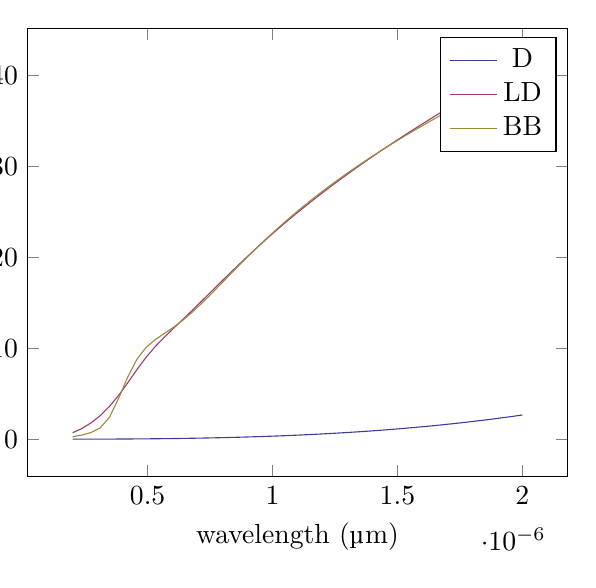
\begin{tikzpicture}[baseline,trim axis left]
			\begin{axis}[xlabel=wavelength (\si{\micro\meter}),ylabel=permittivity $\epsilon''$]
				\addplot[color=colora] coordinates {
						(2e-07, 0.0027067342300210223)
						(2.3673469387755102e-07, 0.004488599792889498)
						(2.7346938775510205e-07, 0.006918560111167206)
						(3.1020408163265303e-07, 0.010096977105621633)
						(3.4693877551020406e-07, 0.014124124447990159)
						(3.836734693877551e-07, 0.019100175772322866)
						(4.2040816326530607e-07, 0.025125192911072153)
						(4.571428571428571e-07, 0.03229911415882458)
						(4.938775510204081e-07, 0.04072174256655862)
						(5.306122448979591e-07, 0.050492734269299386)
						(5.673469387755102e-07, 0.06171158685002681)
						(6.040816326530612e-07, 0.07447762774267892)
						(6.408163265306121e-07, 0.08889000267707461)
						(6.775510204081632e-07, 0.10504766416856431)
						(7.142857142857142e-07, 0.12304936005519528)
						(7.510204081632653e-07, 0.1429936220851614)
						(7.877551020408163e-07, 0.16497875455728372)
						(8.244897959183672e-07, 0.18910282301724804)
						(8.612244897959183e-07, 0.21546364301229956)
						(8.979591836734693e-07, 0.2441587689070726)
						(9.346938775510204e-07, 0.27528548276320824)
						(9.714285714285713e-07, 0.3089407832853824)
						(1.0081632653061223e-06, 0.34522137483634474)
						(1.0448979591836734e-06, 0.38422365652353463)
						(1.0816326530612245e-06, 0.4260437113598151)
						(1.1183673469387754e-06, 0.4707772955008306)
						(1.1551020408163265e-06, 0.518519827561472)
						(1.1918367346938776e-06, 0.5693663780138815)
						(1.2285714285714284e-06, 0.6234116586694198)
						(1.2653061224489795e-06, 0.6807500122469661)
						(1.3020408163265306e-06, 0.7414754020298908)
						(1.3387755102040815e-06, 0.8056814016140071)
						(1.3755102040816325e-06, 0.8734611847487738)
						(1.4122448979591836e-06, 0.9449075152739669)
						(1.4489795918367345e-06, 1.0201127371540242)
						(1.4857142857142856e-06, 1.0991687646122115)
						(1.5224489795918367e-06, 1.1821670723667115)
						(1.5591836734693875e-06, 1.2691986859707194)
						(1.5959183673469386e-06, 1.3603541722585686)
						(1.6326530612244897e-06, 1.455723629899872)
						(1.6693877551020408e-06, 1.5553966800636203)
						(1.7061224489795917e-06, 1.6594624571941488)
						(1.7428571428571427e-06, 1.7680095999008134)
						(1.7795918367346938e-06, 1.8811262419631964)
						(1.8163265306122447e-06, 1.9989000034536029)
						(1.8530612244897958e-06, 2.1214179819785803)
						(1.8897959183673469e-06, 2.248766744041108)
						(1.9265306122448977e-06, 2.3810323165251135)
						(1.963265306122449e-06, 2.5183001783038845)
						(2e-06, 2.6606552519738877)
					};
				\addlegendentry{D}
				\addplot[color=colorb] coordinates {
						(2e-07, 0.7175631887985846)
						(2.3673469387755102e-07, 1.17491862598837)
						(2.7346938775510205e-07, 1.7899275424019934)
						(3.1020408163265303e-07, 2.5866740773650765)
						(3.4693877551020406e-07, 3.5882130150048743)
						(3.836734693877551e-07, 4.802998247287023)
						(4.2040816326530607e-07, 6.193044419116592)
						(4.571428571428571e-07, 7.6436644874632895)
						(4.938775510204081e-07, 9.00113380419043)
						(5.306122448979591e-07, 10.183089082012978)
						(5.673469387755102e-07, 11.221703177744702)
						(6.040816326530612e-07, 12.194206791410418)
						(6.408163265306121e-07, 13.156671175028833)
						(6.775510204081632e-07, 14.131997612382133)
						(7.142857142857142e-07, 15.122272315593495)
						(7.510204081632653e-07, 16.120866075801224)
						(7.877551020408163e-07, 17.119131615542216)
						(8.244897959183672e-07, 18.109262778700053)
						(8.612244897959183e-07, 19.085207774504855)
						(8.979591836734693e-07, 20.042738636471675)
						(9.346938775510204e-07, 20.979205158412856)
						(9.714285714285713e-07, 21.893205550395763)
						(1.0081632653061223e-06, 22.784269081028118)
						(1.0448979591836734e-06, 23.65258503397978)
						(1.0816326530612245e-06, 24.498785764520665)
						(1.1183673469387754e-06, 25.3237805471335)
						(1.1551020408163265e-06, 26.128632821432657)
						(1.1918367346938776e-06, 26.91447255667828)
						(1.2285714285714284e-06, 27.682435982946103)
						(1.2653061224489795e-06, 28.433626019121878)
						(1.3020408163265306e-06, 29.169087943754928)
						(1.3387755102040815e-06, 29.889796004912494)
						(1.3755102040816325e-06, 30.59664766519296)
						(1.4122448979591836e-06, 31.290463003955765)
						(1.4489795918367345e-06, 31.971987456970837)
						(1.4857142857142856e-06, 32.641896584137356)
						(1.5224489795918367e-06, 33.300801943228045)
						(1.5591836734693875e-06, 33.949257436006576)
						(1.5959183673469386e-06, 34.58776570415862)
						(1.6326530612244897e-06, 35.21678430445647)
						(1.6693877551020408e-06, 35.83673150014647)
						(1.7061224489795917e-06, 36.44799158026606)
						(1.7428571428571427e-06, 37.05091966934993)
						(1.7795918367346938e-06, 37.64584602349137)
						(1.8163265306122447e-06, 38.23307982998857)
						(1.8530612244897958e-06, 38.812912540507504)
						(1.8897959183673469e-06, 39.38562077450942)
						(1.9265306122448977e-06, 39.95146883254614)
						(1.963265306122449e-06, 40.510710859289595)
						(2e-06, 41.06359269479416)
					};
				\addlegendentry{LD}
				\addplot[color=colorc] coordinates {
						(2e-07, 0.2688426232193136)
						(2.3673469387755102e-07, 0.45686323502196413)
						(2.7346938775510205e-07, 0.7341919401724433)
						(3.1020408163265303e-07, 1.235549019350498)
						(3.4693877551020406e-07, 2.4032664540063684)
						(3.836734693877551e-07, 4.46584864089719)
						(4.2040816326530607e-07, 6.834478321442088)
						(4.571428571428571e-07, 8.781058621136728)
						(4.938775510204081e-07, 10.091910751100729)
						(5.306122448979591e-07, 10.953926346484533)
						(5.673469387755102e-07, 11.63296399028786)
						(6.040816326530612e-07, 12.311964945491072)
						(6.408163265306121e-07, 13.07351325837416)
						(6.775510204081632e-07, 13.933626439376402)
						(7.142857142857142e-07, 14.87617908115999)
						(7.510204081632653e-07, 15.87475859791324)
						(7.877551020408163e-07, 16.903508418261207)
						(8.244897959183672e-07, 17.941273888253043)
						(8.612244897959183e-07, 18.97239700179424)
						(8.979591836734693e-07, 19.98611750057188)
						(9.346938775510204e-07, 20.975560172983826)
						(9.714285714285713e-07, 21.936735006147583)
						(1.0081632653061223e-06, 22.867700841915283)
						(1.0448979591836734e-06, 23.767919648436227)
						(1.0816326530612245e-06, 24.637780707351286)
						(1.1183673469387754e-06, 25.478260702238792)
						(1.1551020408163265e-06, 26.290686495026364)
						(1.1918367346938776e-06, 27.076572899253268)
						(1.2285714285714284e-06, 27.837514014226336)
						(1.2653061224489795e-06, 28.575112196725545)
						(1.3020408163265306e-06, 29.29093313586239)
						(1.3387755102040815e-06, 29.986478812289363)
						(1.3755102040816325e-06, 30.66317255267375)
						(1.4122448979591836e-06, 31.3223521377057)
						(1.4489795918367345e-06, 31.96526816331877)
						(1.4857142857142856e-06, 32.59308572947833)
						(1.5224489795918367e-06, 33.20688814348632)
						(1.5591836734693875e-06, 33.80768175172213)
						(1.5959183673469386e-06, 34.39640131002334)
						(1.6326530612244897e-06, 34.97391550754844)
						(1.6693877551020408e-06, 35.5410323995258)
						(1.7061224489795917e-06, 36.098504600160716)
						(1.7428571428571427e-06, 36.647034151742574)
						(1.7795918367346938e-06, 37.187277029188174)
						(1.8163265306122447e-06, 37.71984726753043)
						(1.8530612244897958e-06, 38.245320717873085)
						(1.8897959183673469e-06, 38.764238448324036)
						(1.9265306122448977e-06, 39.27710981266158)
						(1.963265306122449e-06, 39.784415212550684)
						(2e-06, 40.28660858010165)
					};
				\addlegendentry{BB}
			\end{axis}
		\end{tikzpicture}%
		\\
		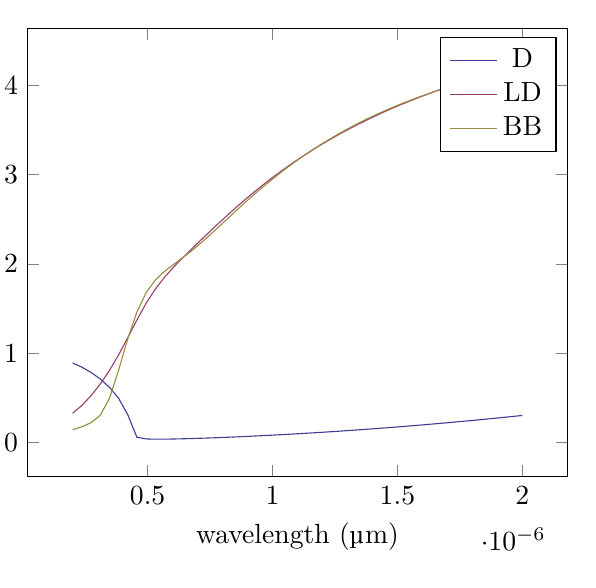
\begin{tikzpicture}[baseline,trim axis left]
			\begin{axis}[xlabel=wavelength (\si{\micro\meter}),ylabel=refractive index $n'$]
				\addplot[color=colora] coordinates {
						(2e-07, 0.8918367942226354)
						(2.3673469387755102e-07, 0.8445853283818916)
						(2.7346938775510205e-07, 0.7858082949439328)
						(3.1020408163265303e-07, 0.7126720654455929)
						(3.4693877551020406e-07, 0.6201473493146706)
						(3.836734693877551e-07, 0.49765206967136355)
						(4.2040816326530607e-07, 0.31301835084887897)
						(4.571428571428571e-07, 0.060218801682668875)
						(4.938775510204081e-07, 0.04085578222905428)
						(5.306122448979591e-07, 0.03804909385979461)
						(5.673469387755102e-07, 0.03838687485547863)
						(6.040816326530612e-07, 0.040021851395341194)
						(6.408163265306121e-07, 0.04239299665295058)
						(6.775510204081632e-07, 0.04526804534128262)
						(7.142857142857142e-07, 0.04853244601682341)
						(7.510204081632653e-07, 0.052122842629139965)
						(7.877551020408163e-07, 0.056001212261970815)
						(8.244897959183672e-07, 0.06014328500711672)
						(8.612244897959183e-07, 0.0645327990653524)
						(8.979591836734693e-07, 0.06915841878187354)
						(9.346938775510204e-07, 0.07401197576247616)
						(9.714285714285713e-07, 0.07908741336216772)
						(1.0081632653061223e-06, 0.08438012632574976)
						(1.0448979591836734e-06, 0.08988653287379558)
						(1.0816326530612245e-06, 0.09560378895498274)
						(1.1183673469387754e-06, 0.1015295924060197)
						(1.1551020408163265e-06, 0.10766204564536881)
						(1.1918367346938776e-06, 0.11399955745772916)
						(1.2285714285714284e-06, 0.12054077147895932)
						(1.2653061224489795e-06, 0.12728451328781998)
						(1.3020408163265306e-06, 0.13422975069961587)
						(1.3387755102040815e-06, 0.14137556357997602)
						(1.3755102040816325e-06, 0.1487211206254926)
						(1.4122448979591836e-06, 0.15626566131150244)
						(1.4489795918367345e-06, 0.16400848171943527)
						(1.4857142857142856e-06, 0.17194892331003028)
						(1.5224489795918367e-06, 0.18008636395674205)
						(1.5591836734693875e-06, 0.18842021072998902)
						(1.5959183673469386e-06, 0.1969498940498637)
						(1.6326530612244897e-06, 0.20567486291730291)
						(1.6693877551020408e-06, 0.21459458100178488)
						(1.7061224489795917e-06, 0.22370852341427452)
						(1.7428571428571427e-06, 0.2330161740320729)
						(1.7795918367346938e-06, 0.24251702327106664)
						(1.8163265306122447e-06, 0.25221056622283156)
						(1.8530612244897958e-06, 0.26209630109098897)
						(1.8897959183673469e-06, 0.2721737278743033)
						(1.9265306122448977e-06, 0.28244234725428896)
						(1.963265306122449e-06, 0.2929016596531641)
						(2e-06, 0.3035511644343023)
					};
				\addlegendentry{D}
				\addplot[color=colorb] coordinates {
						(2e-07, 0.3289245060036228)
						(2.3673469387755102e-07, 0.4152672994580423)
						(2.7346938775510205e-07, 0.5241646948406355)
						(3.1020408163265303e-07, 0.6539158936685996)
						(3.4693877551020406e-07, 0.8055796231761215)
						(3.836734693877551e-07, 0.9799383830287132)
						(4.2040816326530607e-07, 1.1732449662108835)
						(4.571428571428571e-07, 1.3726163690031086)
						(4.938775510204081e-07, 1.5584785887507564)
						(5.306122448979591e-07, 1.7171593808367247)
						(5.673469387755102e-07, 1.849173069371164)
						(6.040816326530612e-07, 1.9635295006390063)
						(6.408163265306121e-07, 2.0689026193023894)
						(6.775510204081632e-07, 2.170341725657233)
						(7.142857142857142e-07, 2.269890480855815)
						(7.510204081632653e-07, 2.367954240184568)
						(7.877551020408163e-07, 2.4642569214575953)
						(8.244897959183672e-07, 2.5583375119950333)
						(8.612244897959183e-07, 2.6497653454070953)
						(8.979591836734693e-07, 2.7382145807150633)
						(9.346938775510204e-07, 2.8234757739233656)
						(9.714285714285713e-07, 2.905442576297369)
						(1.0081632653061223e-06, 2.9840909043740993)
						(1.0448979591836734e-06, 3.059457997851334)
						(1.0816326530612245e-06, 3.1316241902643775)
						(1.1183673469387754e-06, 3.2006981560521086)
						(1.1551020408163265e-06, 3.2668055170260875)
						(1.1918367346938776e-06, 3.3300803578982046)
						(1.2285714285714284e-06, 3.390659117032923)
						(1.2653061224489795e-06, 3.4486763442121937)
						(1.3020408163265306e-06, 3.504261884912342)
						(1.3387755102040815e-06, 3.557539128761728)
						(1.3755102040816325e-06, 3.6086240341687947)
						(1.4122448979591836e-06, 3.657624705849554)
						(1.4489795918367345e-06, 3.7046413556210154)
						(1.4857142857142856e-06, 3.749766519825884)
						(1.5224489795918367e-06, 3.79308544041144)
						(1.5591836734693875e-06, 3.8346765425450204)
						(1.5959183673469386e-06, 3.874611961210796)
						(1.6326530612244897e-06, 3.912958083829334)
						(1.6693877551020408e-06, 3.949776086693311)
						(1.7061224489795917e-06, 3.9851224508307115)
						(1.7428571428571427e-06, 4.0190494485136705)
						(1.7795918367346938e-06, 4.051605595589768)
						(1.8163265306122447e-06, 4.082836067555194)
						(1.8530612244897958e-06, 4.112783079143782)
						(1.8897959183673469e-06, 4.141486228418697)
						(1.9265306122448977e-06, 4.168982807108011)
						(1.963265306122449e-06, 4.195308079356758)
						(2e-06, 4.220495531275716)
					};
				\addlegendentry{LD}
				\addplot[color=colorc] coordinates {
						(2e-07, 0.1442552594305267)
						(2.3673469387755102e-07, 0.1762372043893419)
						(2.7346938775510205e-07, 0.2224893758468798)
						(3.1020408163265303e-07, 0.3035469309379392)
						(3.4693877551020406e-07, 0.49211856106039265)
						(3.836734693877551e-07, 0.8069351541718742)
						(4.2040816326530607e-07, 1.1601737008033648)
						(4.571428571428571e-07, 1.46147150840941)
						(4.938775510204081e-07, 1.6773364324735975)
						(5.306122448979591e-07, 1.8194906880417492)
						(5.673469387755102e-07, 1.916493962162782)
						(6.040816326530612e-07, 1.9944648594170822)
						(6.408163265306121e-07, 2.0698794409468952)
						(6.775510204081632e-07, 2.150097989701634)
						(7.142857142857142e-07, 2.2366598122976504)
						(7.510204081632653e-07, 2.3283383732484766)
						(7.877551020408163e-07, 2.423044475970889)
						(8.244897959183672e-07, 2.5187442434705893)
						(8.612244897959183e-07, 2.613792428944421)
						(8.979591836734693e-07, 2.7069857421261116)
						(9.346938775510204e-07, 2.7975071966116407)
						(9.714285714285713e-07, 2.8848421953811996)
						(1.0081632653061223e-06, 2.9686989519494786)
						(1.0448979591836734e-06, 3.048943461057844)
						(1.0816326530612245e-06, 3.1255499904371673)
						(1.1183673469387754e-06, 3.198564861480599)
						(1.1551020408163265e-06, 3.26808061410123)
						(1.1918367346938776e-06, 3.334217912541209)
						(1.2285714285714284e-06, 3.3971130675039545)
						(1.2653061224489795e-06, 3.4569095650118866)
						(1.3020408163265306e-06, 3.513752421190251)
						(1.3387755102040815e-06, 3.567784512798963)
						(1.3755102040816325e-06, 3.6191442782987693)
						(1.4122448979591836e-06, 3.6679643617218605)
						(1.4489795918367345e-06, 3.7143708985487334)
						(1.4857142857142856e-06, 3.7584832328827718)
						(1.5224489795918367e-06, 3.8004139188718304)
						(1.5591836734693875e-06, 3.840268904190361)
						(1.5959183673469386e-06, 3.878147824963171)
						(1.6326530612244897e-06, 3.9141443636955353)
						(1.6693877551020408e-06, 3.948346637341947)
						(1.7061224489795917e-06, 3.9808375935497047)
						(1.7428571428571427e-06, 4.011695400729161)
						(1.7795918367346938e-06, 4.040993822899256)
						(1.8163265306122447e-06, 4.068802573918059)
						(1.8530612244897958e-06, 4.095187648216449)
						(1.8897959183673469e-06, 4.120211626849515)
						(1.9265306122448977e-06, 4.143933958806657)
						(1.963265306122449e-06, 4.166411218248403)
						(2e-06, 4.18769733878723)
					};
				\addlegendentry{BB}
			\end{axis}
		\end{tikzpicture}%
		\\
		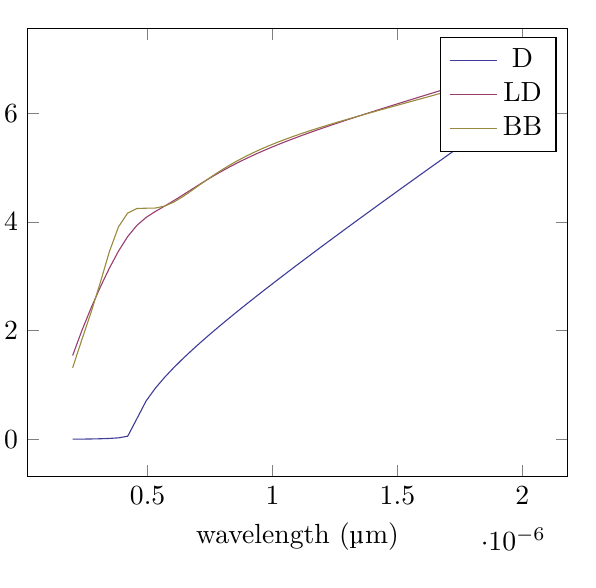
\begin{tikzpicture}[baseline,trim axis left]
			\begin{axis}[xlabel=wavelength (\si{\micro\meter}),ylabel=refractive index $n''$]
				\addplot[color=colora] coordinates {
						(2e-07, 0.0021460766603571455)
						(2.3673469387755102e-07, 0.0037579617416050285)
						(2.7346938775510205e-07, 0.006225641549125486)
						(3.1020408163265303e-07, 0.010018129413287526)
						(3.4693877551020406e-07, 0.016104663168411734)
						(3.836734693877551e-07, 0.027139169378685577)
						(4.2040816326530607e-07, 0.056757676468037366)
						(4.571428571428571e-07, 0.37926564477945085)
						(4.938775510204081e-07, 0.7047869050483953)
						(5.306122448979591e-07, 0.9383601862907733)
						(5.673469387755102e-07, 1.1367604605408141)
						(6.040816326530612e-07, 1.3158720495790635)
						(6.408163265306121e-07, 1.482667625202529)
						(6.775510204081632e-07, 1.6408907237189263)
						(7.142857142857142e-07, 1.79280139487575)
						(7.510204081632653e-07, 1.9398742421296244)
						(7.877551020408163e-07, 2.083126264364592)
						(8.244897959183672e-07, 2.223288742561934)
						(8.612244897959183e-07, 2.360904924004038)
						(8.979591836734693e-07, 2.496389076286982)
						(9.346938775510204e-07, 2.6300639811154425)
						(9.714285714285713e-07, 2.7621857076776775)
						(1.0081632653061223e-06, 2.89296053213929)
						(1.0448979591836734e-06, 3.0225568206256375)
						(1.0816326530612245e-06, 3.151113576955227)
						(1.1183673469387754e-06, 3.278746719932318)
						(1.1551020408163265e-06, 3.4055537775690636)
						(1.1918367346938776e-06, 3.531617454063555)
						(1.2285714285714284e-06, 3.657008379051611)
						(1.2653061224489795e-06, 3.7817872537578987)
						(1.3020408163265306e-06, 3.906006545684929)
						(1.3387755102040815e-06, 4.029711840793934)
						(1.3755102040816325e-06, 4.152942932661164)
						(1.4122448979591836e-06, 4.275734707399664)
						(1.4489795918367345e-06, 4.398117868381586)
						(1.4857142857142856e-06, 4.520119534126765)
						(1.5224489795918367e-06, 4.641763734908576)
						(1.5591836734693875e-06, 4.763071827836123)
						(1.5959183673469386e-06, 4.884062845831796)
						(1.6326530612244897e-06, 5.004753792638135)
						(1.6693877551020408e-06, 5.125159893477846)
						(1.7061224489795917e-06, 5.245294809055984)
						(1.7428571428571427e-06, 5.365170819089597)
						(1.7795918367346938e-06, 5.484798980372613)
						(1.8163265306122447e-06, 5.604189263454826)
						(1.8530612244897958e-06, 5.723350671276232)
						(1.8897959183673469e-06, 5.842291342508353)
						(1.9265306122448977e-06, 5.961018641880241)
						(1.963265306122449e-06, 6.079539239383505)
						(2e-06, 6.197859179939056)
					};
				\addlegendentry{D}
				\addplot[color=colorb] coordinates {
						(2e-07, 1.5425843543677273)
						(2.3673469387755102e-07, 2.0006220785094553)
						(2.7346938775510205e-07, 2.414641648937895)
						(3.1020408163265303e-07, 2.7970795610471195)
						(3.4693877551020406e-07, 3.1495952507441487)
						(3.836734693877551e-07, 3.465761408576485)
						(4.2040816326530607e-07, 3.732505854331295)
						(4.571428571428571e-07, 3.937653021088114)
						(4.938775510204081e-07, 4.083959059336436)
						(5.306122448979591e-07, 4.193280730766792)
						(5.673469387755102e-07, 4.291076127419641)
						(6.040816326530612e-07, 4.391381087267208)
						(6.408163265306121e-07, 4.496669547859819)
						(6.775510204081632e-07, 4.604266335247934)
						(7.142857142857142e-07, 4.710826972266149)
						(7.510204081632653e-07, 4.81393327934864)
						(7.877551020408163e-07, 4.912253242740143)
						(8.244897959183672e-07, 5.00527489163158)
						(8.612244897959183e-07, 5.0930094097193574)
						(8.979591836734693e-07, 5.175765443370673)
						(9.346938775510204e-07, 5.253998765785113)
						(9.714285714285713e-07, 5.328218920204656)
						(1.0081632653061223e-06, 5.398934445314147)
						(1.0448979591836734e-06, 5.466622938397746)
						(1.0816326530612245e-06, 5.531716608520179)
						(1.1183673469387754e-06, 5.59459720258187)
						(1.1551020408163265e-06, 5.65559637844241)
						(1.1918367346938776e-06, 5.71499904251506)
						(1.2285714285714284e-06, 5.773048108838719)
						(1.2653061224489795e-06, 5.8299497445116755)
						(1.3020408163265306e-06, 5.885878556868137)
						(1.3387755102040815e-06, 5.940982425880653)
						(1.3755102040816325e-06, 5.995386840185717)
						(1.4122448979591836e-06, 6.0491986892965794)
						(1.4489795918367345e-06, 6.102509519452677)
						(1.4857142857142856e-06, 6.155398290372831)
						(1.5224489795918367e-06, 6.207933684312822)
						(1.5591836734693875e-06, 6.260176023429552)
						(1.5959183673469386e-06, 6.312178850513664)
						(1.6326530612244897e-06, 6.363990224218117)
						(1.6693877551020408e-06, 6.415653774573761)
						(1.7061224489795917e-06, 6.467209558808897)
						(1.7428571428571427e-06, 6.518694751835984)
						(1.7795918367346938e-06, 6.570144200534038)
						(1.8163265306122447e-06, 6.62159086627743)
						(1.8530612244897958e-06, 6.673066176081149)
						(1.8897959183673469e-06, 6.724600299233881)
						(1.9265306122448977e-06, 6.776222363328269)
						(1.963265306122449e-06, 6.8279606211144355)
						(2e-06, 6.879842577536054)
					};
				\addlegendentry{LD}
				\addplot[color=colorc] coordinates {
						(2e-07, 1.3178059690912607)
						(2.3673469387755102e-07, 1.833047072428431)
						(2.7346938775510205e-07, 2.33337927985258)
						(3.1020408163265303e-07, 2.87818785507585)
						(3.4693877551020406e-07, 3.453163812729075)
						(3.836734693877551e-07, 3.913365084424768)
						(4.2040816326530607e-07, 4.165502082677565)
						(4.571428571428571e-07, 4.248557745583483)
						(4.938775510204081e-07, 4.254399051422902)
						(5.306122448979591e-07, 4.257013048279733)
						(5.673469387755102e-07, 4.292081209349925)
						(6.040816326530612e-07, 4.365017443943457)
						(6.408163265306121e-07, 4.466139281377488)
						(6.775510204081632e-07, 4.582378007418372)
						(7.142857142857142e-07, 4.703016099541665)
						(7.510204081632653e-07, 4.821098850259756)
						(7.877551020408163e-07, 4.932879089479822)
						(8.244897959183672e-07, 5.036794212987746)
						(8.612244897959183e-07, 5.132584526136177)
						(8.979591836734693e-07, 5.220684761769652)
						(9.346938775510204e-07, 5.301849037410127)
						(9.714285714285713e-07, 5.37693677136804)
						(1.0081632653061223e-06, 5.446798950376967)
						(1.0448979591836734e-06, 5.512223290711716)
						(1.0816326530612245e-06, 5.573912388174106)
						(1.1183673469387754e-06, 5.632479469887108)
						(1.1551020408163265e-06, 5.68845291712467)
						(1.1918367346938776e-06, 5.742284640826471)
						(1.2285714285714284e-06, 5.7943596635416)
						(1.2653061224489795e-06, 5.84500555408703)
						(1.3020408163265306e-06, 5.894501081733614)
						(1.3387755102040815e-06, 5.943083848256874)
						(1.3755102040816325e-06, 5.9909568609076915)
						(1.4122448979591836e-06, 6.038294109511891)
						(1.4489795918367345e-06, 6.0852452536607125)
						(1.4857142857142856e-06, 6.131939538128957)
						(1.5224489795918367e-06, 6.1784890513538375)
						(1.5591836734693875e-06, 6.224991431395456)
						(1.5959183673469386e-06, 6.27153211081177)
						(1.6326530612244897e-06, 6.31818617867323)
						(1.6693877551020408e-06, 6.365019925655271)
						(1.7061224489795917e-06, 6.412092127251638)
						(1.7428571428571427e-06, 6.459455110764934)
						(1.7795918367346938e-06, 6.50715564379056)
						(1.8163265306122447e-06, 6.555235675273336)
						(1.8530612244897958e-06, 6.603732954713446)
						(1.8897959183673469e-06, 6.652681550559428)
						(1.9265306122448977e-06, 6.702112285095298)
						(1.963265306122449e-06, 6.752053100068863)
						(2e-06, 6.802529364800734)
					};
				\addlegendentry{BB}
			\end{axis}
		\end{tikzpicture}%
		\\
	\end{tabular}
	\caption{Complex permittivity $\epsilon = \epsilon' + \mi \epsilon''$ and refractive index $n = n' + \mi n''$ for Ti based on the Drude (D), Lorentz-Drude (LD), and Brendel-Bormann (BB) models.}
\end{figure}
\clearpage
\newpage
\subsection{Be}
\begin{figure}[h!]
	\centering
	\begin{tabular}{l}
		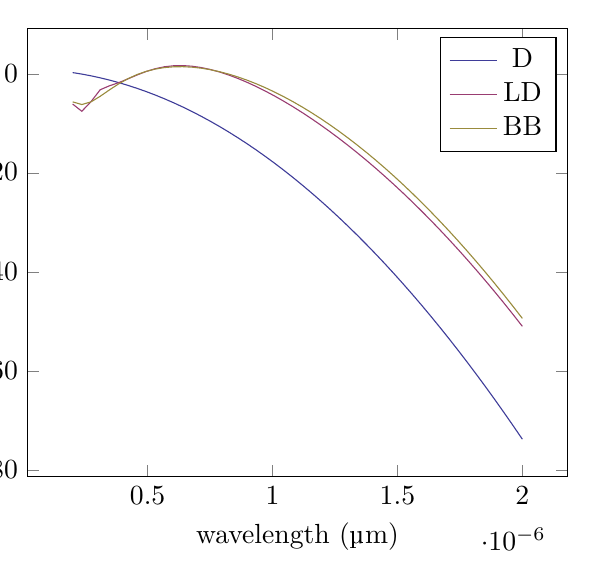
\begin{tikzpicture}[baseline,trim axis left]
			\begin{axis}[xlabel=wavelength (\si{\micro\meter}),ylabel=permittivity $\epsilon'$]
				\addplot[color=colora] coordinates {
						(2e-07, 0.25113144608801274)
						(2.3673469387755102e-07, -0.049213498185279425)
						(2.7346938775510205e-07, -0.4000740344521363)
						(3.1020408163265303e-07, -0.8014456357912376)
						(3.4693877551020406e-07, -1.2533231238191513)
						(3.836734693877551e-07, -1.7557006688573384)
						(4.2040816326530607e-07, -2.308571790120155)
						(4.571428571428571e-07, -2.911929355923831)
						(4.938775510204081e-07, -3.565765583916411)
						(5.306122448979591e-07, -4.270072041328657)
						(5.673469387755102e-07, -5.024839645245882)
						(6.040816326530612e-07, -5.830058662900699)
						(6.408163265306121e-07, -6.68571871198669)
						(6.775510204081632e-07, -7.591808760992944)
						(7.142857142857142e-07, -8.548317129559468)
						(7.510204081632653e-07, -9.555231488853433)
						(7.877551020408163e-07, -10.612538861966252)
						(8.244897959183672e-07, -11.720225624331452)
						(8.612244897959183e-07, -12.878277504163309)
						(8.979591836734693e-07, -14.086679582916224)
						(9.346938775510204e-07, -15.345416295764846)
						(9.714285714285713e-07, -16.65447143210484)
						(1.0081632653061223e-06, -18.01382813607438)
						(1.0448979591836734e-06, -19.423468907096158)
						(1.0816326530612245e-06, -20.883375600440136)
						(1.1183673469387754e-06, -22.393529427806698)
						(1.1551020408163265e-06, -23.95391095793051)
						(1.1918367346938776e-06, -25.564500117204677)
						(1.2285714285714284e-06, -27.225276190325474)
						(1.2653061224489795e-06, -28.936217820957513)
						(1.3020408163265306e-06, -30.69730301241917)
						(1.3387755102040815e-06, -32.508509128388425)
						(1.3755102040816325e-06, -34.36981289362904)
						(1.4122448979591836e-06, -36.28119039473681)
						(1.4489795918367345e-06, -38.242617080906214)
						(1.4857142857142856e-06, -40.254067764717135)
						(1.5224489795918367e-06, -42.31551662294167)
						(1.5591836734693875e-06, -44.42693719737102)
						(1.5959183673469386e-06, -46.588302395662424)
						(1.6326530612244897e-06, -48.799584492206044)
						(1.6693877551020408e-06, -51.06075512901165)
						(1.7061224489795917e-06, -53.37178531661544)
						(1.7428571428571427e-06, -55.73264543500628)
						(1.7795918367346938e-06, -58.14330523457212)
						(1.8163265306122447e-06, -60.603733837065604)
						(1.8530612244897958e-06, -63.113899736589914)
						(1.8897959183673469e-06, -65.6737708006036)
						(1.9265306122448977e-06, -68.2833142709453)
						(1.963265306122449e-06, -70.94249676487787)
						(2e-06, -73.65128427615174)
					};
				\addlegendentry{D}
				\addplot[color=colorb] coordinates {
						(2e-07, -6.0884552678196675)
						(2.3673469387755102e-07, -7.54631795292425)
						(2.7346938775510205e-07, -5.610827277812885)
						(3.1020408163265303e-07, -3.211715205178544)
						(3.4693877551020406e-07, -2.4169316229654316)
						(3.836734693877551e-07, -1.7894389245478357)
						(4.2040816326530607e-07, -1.0358276378596503)
						(4.571428571428571e-07, -0.2459608659479704)
						(4.938775510204081e-07, 0.4679465527303659)
						(5.306122448979591e-07, 1.0351717940899459)
						(5.673469387755102e-07, 1.4246481705391876)
						(6.040816326530612e-07, 1.6313982552369417)
						(6.408163265306121e-07, 1.6645165726082922)
						(6.775510204081632e-07, 1.5391693620849853)
						(7.142857142857142e-07, 1.2720110596150036)
						(7.510204081632653e-07, 0.878872391192699)
						(7.877551020408163e-07, 0.37377957812082485)
						(8.244897959183672e-07, -0.2313153020433525)
						(8.612244897959183e-07, -0.9264587848801877)
						(8.979591836734693e-07, -1.7034760078362439)
						(9.346938775510204e-07, -2.5557093082535722)
						(9.714285714285713e-07, -3.4777643342325106)
						(1.0081632653061223e-06, -4.46528392680033)
						(1.0448979591836734e-06, -5.514755645531757)
						(1.0816326530612245e-06, -6.623352080740016)
						(1.1183673469387754e-06, -7.788800331988018)
						(1.1551020408163265e-06, -9.009276234839092)
						(1.1918367346938776e-06, -10.283319030835976)
						(1.2285714285714284e-06, -11.609762659787714)
						(1.2653061224489795e-06, -12.987680443095634)
						(1.3020408163265306e-06, -14.416340499859015)
						(1.3387755102040815e-06, -15.895169744515488)
						(1.3755102040816325e-06, -17.423724742075855)
						(1.4122448979591836e-06, -19.0016680472112)
						(1.4489795918367345e-06, -20.62874893567322)
						(1.4857142857142856e-06, -22.304787661662907)
						(1.5224489795918367e-06, -24.029662553279238)
						(1.5591836734693875e-06, -25.803299399269502)
						(1.5959183673469386e-06, -27.625662691659063)
						(1.6326530612244897e-06, -29.496748376718834)
						(1.6693877551020408e-06, -31.416577836142906)
						(1.7061224489795917e-06, -33.3851928752177)
						(1.7428571428571427e-06, -35.40265153828466)
						(1.7795918367346938e-06, -37.469024606374056)
						(1.8163265306122447e-06, -39.5843926594236)
						(1.8530612244897958e-06, -41.7488436074891)
						(1.8897959183673469e-06, -43.962470612965596)
						(1.9265306122448977e-06, -46.22537033998662)
						(1.963265306122449e-06, -48.53764147856573)
						(2e-06, -50.899383500253904)
					};
				\addlegendentry{LD}
				\addplot[color=colorc] coordinates {
						(2e-07, -5.649127791979251)
						(2.3673469387755102e-07, -6.187836124745447)
						(2.7346938775510205e-07, -5.652143771533121)
						(3.1020408163265303e-07, -4.5304931601141885)
						(3.4693877551020406e-07, -3.2486752826113836)
						(3.836734693877551e-07, -2.0391942214777905)
						(4.2040816326530607e-07, -0.9993217482899968)
						(4.571428571428571e-07, -0.156833987262039)
						(4.938775510204081e-07, 0.49103749265274255)
						(5.306122448979591e-07, 0.9584768296958721)
						(5.673469387755102e-07, 1.2625275104514984)
						(6.040816326530612e-07, 1.419580270358468)
						(6.408163265306121e-07, 1.4441385738400436)
						(6.775510204081632e-07, 1.348564070113806)
						(7.142857142857142e-07, 1.143212130213131)
						(7.510204081632653e-07, 0.8366963507724687)
						(7.877551020408163e-07, 0.43617124178034494)
						(8.244897959183672e-07, -0.05240986105181378)
						(8.612244897959183e-07, -0.6240747189786742)
						(8.979591836734693e-07, -1.2746504548339352)
						(9.346938775510204e-07, -2.0006159570640634)
						(9.714285714285713e-07, -2.798982961947498)
						(1.0081632653061223e-06, -3.667200522697568)
						(1.0448979591836734e-06, -4.603078255768615)
						(1.0816326530612245e-06, -5.604724546360183)
						(1.1183673469387754e-06, -6.670496633909234)
						(1.1551020408163265e-06, -7.798960129675841)
						(1.1918367346938776e-06, -8.988856034825643)
						(1.2285714285714284e-06, -10.239073739695142)
						(1.2653061224489795e-06, -11.548628809827036)
						(1.3020408163265306e-06, -12.91664461861549)
						(1.3387755102040815e-06, -14.342337084737586)
						(1.3755102040816325e-06, -15.825001927165527)
						(1.4122448979591836e-06, -17.364003971206873)
						(1.4489795918367345e-06, -18.958768133373294)
						(1.4857142857142856e-06, -20.60877178687262)
						(1.5224489795918367e-06, -22.313538267752524)
						(1.5591836734693875e-06, -24.072631327720845)
						(1.5959183673469386e-06, -25.885650376149076)
						(1.6326530612244897e-06, -27.752226382816747)
						(1.6693877551020408e-06, -29.672018336189545)
						(1.7061224489795917e-06, -31.64471017068396)
						(1.7428571428571427e-06, -33.67000809142156)
						(1.7795918367346938e-06, -35.74763823716627)
						(1.8163265306122447e-06, -37.87734463205237)
						(1.8530612244897958e-06, -40.05888738480703)
						(1.8897959183673469e-06, -42.292041100809286)
						(1.9265306122448977e-06, -44.57659347779203)
						(1.963265306122449e-06, -46.912344060507266)
						(2e-06, -49.29910313341995)
					};
				\addlegendentry{BB}
			\end{axis}
		\end{tikzpicture}%
		\\
		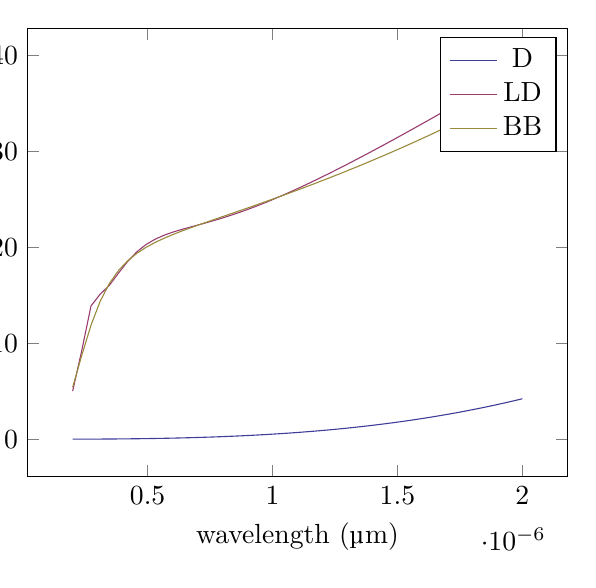
\begin{tikzpicture}[baseline,trim axis left]
			\begin{axis}[xlabel=wavelength (\si{\micro\meter}),ylabel=permittivity $\epsilon''$]
				\addplot[color=colora] coordinates {
						(2e-07, 0.00422802255741341)
						(2.3673469387755102e-07, 0.007011767128826397)
						(2.7346938775510205e-07, 0.010808400412969103)
						(3.1020408163265303e-07, 0.015775036548467656)
						(3.4693877551020406e-07, 0.02206876451596727)
						(3.836734693877551e-07, 0.029846644762114828)
						(4.2040816326530607e-07, 0.039265705824829834)
						(4.571428571428571e-07, 0.05048294096001578)
						(4.938775510204081e-07, 0.06365530476986397)
						(5.306122448979591e-07, 0.07893970983290216)
						(5.673469387755102e-07, 0.0964930233359394)
						(6.040816326530612e-07, 0.11647206370805903)
						(6.408163265306121e-07, 0.13903359725681136)
						(6.775510204081632e-07, 0.16433433480675735)
						(7.142857142857142e-07, 0.192530928340515)
						(7.510204081632653e-07, 0.2237799676424576)
						(7.877551020408163e-07, 0.25823797694521794)
						(8.244897959183672e-07, 0.29606141157914573)
						(8.612244897959183e-07, 0.3374066546248709)
						(8.979591836734693e-07, 0.3824300135691202)
						(9.346938775510204e-07, 0.43128771696394197)
						(9.714285714285713e-07, 0.48413591108948145)
						(1.0081632653061223e-06, 0.5411306566204642)
						(1.0448979591836734e-06, 0.6024279252965284)
						(1.0816326530612245e-06, 0.6681835965965627)
						(1.1183673469387754e-06, 0.7385534544171884)
						(1.1551020408163265e-06, 0.8136931837555491)
						(1.1918367346938776e-06, 0.893758367396536)
						(1.2285714285714284e-06, 0.9789044826046126)
						(1.2653061224489795e-06, 1.069286897820381)
						(1.3020408163265306e-06, 1.1650608693620303)
						(1.3387755102040815e-06, 1.2663815381318217)
						(1.3755102040816325e-06, 1.3734039263277567)
						(1.4122448979591836e-06, 1.4862829341605597)
						(1.4489795918367345e-06, 1.6051733365761427)
						(1.4857142857142856e-06, 1.7302297799836805)
						(1.5224489795918367e-06, 1.8616067789894417)
						(1.5591836734693875e-06, 1.9994587131365265)
						(1.5959183673469386e-06, 2.1439398236506526)
						(1.6326530612244897e-06, 2.2952042101921273)
						(1.6693877551020408e-06, 2.453405827614147)
						(1.7061224489795917e-06, 2.618698482727589)
						(1.7428571428571427e-06, 2.7912358310723935)
						(1.7795918367346938e-06, 2.971171373695724)
						(1.8163265306122447e-06, 3.1586584539370057)
						(1.8530612244897958e-06, 3.3538502542200233)
						(1.8897959183673469e-06, 3.556899792852171)
						(1.9265306122448977e-06, 3.7679599208310277)
						(1.963265306122449e-06, 3.9871833186584023)
						(2e-06, 4.214722493161938)
					};
				\addlegendentry{D}
				\addplot[color=colorb] coordinates {
						(2e-07, 5.009510356940894)
						(2.3673469387755102e-07, 9.271419355486051)
						(2.7346938775510205e-07, 13.894146312783137)
						(3.1020408163265303e-07, 15.115123065491867)
						(3.4693877551020406e-07, 16.04171349112017)
						(3.836734693877551e-07, 17.315439957503038)
						(4.2040816326530607e-07, 18.53742950082132)
						(4.571428571428571e-07, 19.535701177370058)
						(4.938775510204081e-07, 20.29383134974853)
						(5.306122448979591e-07, 20.85570991455221)
						(5.673469387755102e-07, 21.278291666263346)
						(6.040816326530612e-07, 21.612317788005814)
						(6.408163265306121e-07, 21.89678429992643)
						(6.775510204081632e-07, 22.159252399589743)
						(7.142857142857142e-07, 22.418070615931274)
						(7.510204081632653e-07, 22.684808200483147)
						(7.877551020408163e-07, 22.96630369022052)
						(8.244897959183672e-07, 23.266211985306622)
						(8.612244897959183e-07, 23.586107925542983)
						(8.979591836734693e-07, 23.926247293035253)
						(9.346938775510204e-07, 24.286080010267955)
						(9.714285714285713e-07, 24.664590474488545)
						(1.0081632653061223e-06, 25.060519882854503)
						(1.0448979591836734e-06, 25.47250909523588)
						(1.0816326530612245e-06, 25.89918850307717)
						(1.1183673469387754e-06, 26.339232834134485)
						(1.1551020408163265e-06, 26.79139293992016)
						(1.1918367346938776e-06, 27.254512617934886)
						(1.2285714285714284e-06, 27.727535830264564)
						(1.2653061224489795e-06, 28.209507876044903)
						(1.3020408163265306e-06, 28.699572868371508)
						(1.3387755102040815e-06, 29.196969059778244)
						(1.3755102040816325e-06, 29.70102302202962)
						(1.4122448979591836e-06, 30.211143326994613)
						(1.4489795918367345e-06, 30.726814136509425)
						(1.4857142857142856e-06, 31.24758895076396)
						(1.5224489795918367e-06, 31.77308466034252)
						(1.5591836734693875e-06, 32.30297597883308)
						(1.5959183673469386e-06, 32.836990288952066)
						(1.6326530612244897e-06, 33.37490290737722)
						(1.6693877551020408e-06, 33.91653275652577)
						(1.7061224489795917e-06, 34.46173842170736)
						(1.7428571428571427e-06, 35.010414566956534)
						(1.7795918367346938e-06, 35.56248868075033)
						(1.8163265306122447e-06, 36.117918122625035)
						(1.8530612244897958e-06, 36.67668744267834)
						(1.8897959183673469e-06, 37.23880594758129)
						(1.9265306122448977e-06, 37.80430548870418)
						(1.963265306122449e-06, 38.37323845007156)
						(2e-06, 38.945675915968685)
					};
				\addlegendentry{LD}
				\addplot[color=colorc] coordinates {
						(2e-07, 5.407164733650091)
						(2.3673469387755102e-07, 8.75794094553034)
						(2.7346938775510205e-07, 11.885762067608468)
						(3.1020408163265303e-07, 14.37651172586184)
						(3.4693877551020406e-07, 16.230189702118743)
						(3.836734693877551e-07, 17.589881706571884)
						(4.2040816326530607e-07, 18.602062370520308)
						(4.571428571428571e-07, 19.379119600966813)
						(4.938775510204081e-07, 19.99937567531205)
						(5.306122448979591e-07, 20.515525227613942)
						(5.673469387755102e-07, 20.96266364656759)
						(6.040816326530612e-07, 21.36419260076843)
						(6.408163265306121e-07, 21.735816754798666)
						(6.775510204081632e-07, 22.088168116908896)
						(7.142857142857142e-07, 22.428514684529702)
						(7.510204081632653e-07, 22.76187461667707)
						(7.877551020408163e-07, 23.09174741520089)
						(8.244897959183672e-07, 23.42059794880249)
						(8.612244897959183e-07, 23.75017997003267)
						(8.979591836734693e-07, 24.081754498156595)
						(9.346938775510204e-07, 24.416238671272833)
						(9.714285714285713e-07, 24.754308152294694)
						(1.0081632653061223e-06, 25.096468198641844)
						(1.0448979591836734e-06, 25.443103383943953)
						(1.0816326530612245e-06, 25.794512640458155)
						(1.1183673469387754e-06, 26.15093411831153)
						(1.1551020408163265e-06, 26.51256292176539)
						(1.1918367346938776e-06, 26.87956382441291)
						(1.2285714285714284e-06, 27.25208041960197)
						(1.2653061224489795e-06, 27.63024172339933)
						(1.3020408163265306e-06, 28.0141669462964)
						(1.3387755102040815e-06, 28.4039689415557)
						(1.3755102040816325e-06, 28.799756692840077)
						(1.4122448979591836e-06, 29.20163710169368)
						(1.4489795918367345e-06, 29.609716263198653)
						(1.4857142857142856e-06, 30.02410036664177)
						(1.5224489795918367e-06, 30.444896321098035)
						(1.5591836734693875e-06, 30.87221217918772)
						(1.5959183673469386e-06, 31.306157412925806)
						(1.6326530612244897e-06, 31.746843081474736)
						(1.6693877551020408e-06, 32.19438192026949)
						(1.7061224489795917e-06, 32.648888373370596)
						(1.7428571428571427e-06, 33.1104785852704)
						(1.7795918367346938e-06, 33.579270364201726)
						(1.8163265306122447e-06, 34.055383125890664)
						(1.8530612244897958e-06, 34.53893782437361)
						(1.8897959183673469e-06, 35.030056874765975)
						(1.9265306122448977e-06, 35.52886407156916)
						(1.963265306122449e-06, 36.035484505128395)
						(2e-06, 36.550044478123176)
					};
				\addlegendentry{BB}
			\end{axis}
		\end{tikzpicture}%
		\\
		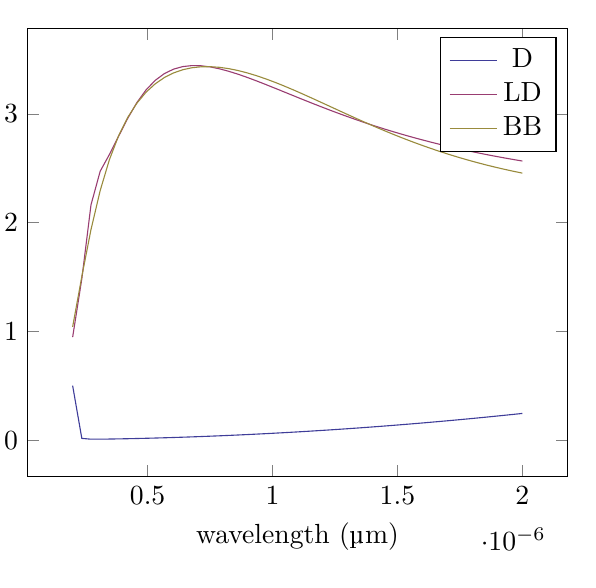
\begin{tikzpicture}[baseline,trim axis left]
			\begin{axis}[xlabel=wavelength (\si{\micro\meter}),ylabel=refractive index $n'$]
				\addplot[color=colora] coordinates {
						(2e-07, 0.5011479227360891)
						(2.3673469387755102e-07, 0.01576382727107637)
						(2.7346938775510205e-07, 0.008543220894360494)
						(3.1020408163265303e-07, 0.008810129964228683)
						(3.4693877551020406e-07, 0.009855976721283424)
						(3.836734693877551e-07, 0.011262235299771134)
						(4.2040816326530607e-07, 0.012920996757993103)
						(4.571428571428571e-07, 0.014791353620563328)
						(4.938775510204081e-07, 0.01685430750323957)
						(5.306122448979591e-07, 0.019099824568302705)
						(5.673469387755102e-07, 0.021522107617268343)
						(6.040816326530612e-07, 0.02411757563216311)
						(6.408163265306121e-07, 0.02688389810372506)
						(6.775510204081632e-07, 0.029819492887264067)
						(7.142857142857142e-07, 0.03292324725955369)
						(7.510204081632653e-07, 0.0361943544864488)
						(7.877551020408163e-07, 0.03963221376665089)
						(8.244897959183672e-07, 0.04323636667275051)
						(8.612244897959183e-07, 0.047006455485731624)
						(8.979591836734693e-07, 0.05094219512940123)
						(9.346938775510204e-07, 0.05504335381226116)
						(9.714285714285713e-07, 0.05930973939351397)
						(1.0081632653061223e-06, 0.06374118960096324)
						(1.0448979591836734e-06, 0.06833756489530048)
						(1.0816326530612245e-06, 0.07309874318659144)
						(1.1183673469387754e-06, 0.07802461586918655)
						(1.1551020408163265e-06, 0.08311508480903947)
						(1.1918367346938776e-06, 0.08837006002925175)
						(1.2285714285714284e-06, 0.09378945791337455)
						(1.2653061224489795e-06, 0.09937319979745024)
						(1.3020408163265306e-06, 0.10512121085716378)
						(1.3387755102040815e-06, 0.11103341922085255)
						(1.3755102040816325e-06, 0.11710975525746838)
						(1.4122448979591836e-06, 0.12335015100080994)
						(1.4489795918367345e-06, 0.1297545396809802)
						(1.4857142857142856e-06, 0.13632285534074656)
						(1.5224489795918367e-06, 0.14305503251971682)
						(1.5591836734693875e-06, 0.14995100599279756)
						(1.5959183673469386e-06, 0.15701071055269808)
						(1.6326530612244897e-06, 0.16423408082815197)
						(1.6693877551020408e-06, 0.17162105113127474)
						(1.7061224489795917e-06, 0.17917155532892817)
						(1.7428571428571427e-06, 0.1868855267339562)
						(1.7795918367346938e-06, 0.19476289801275606)
						(1.8163265306122447e-06, 0.20280360110654647)
						(1.8530612244897958e-06, 0.2110075671641934)
						(1.8897959183673469e-06, 0.21937472648454442)
						(1.9265306122448977e-06, 0.2279050084669386)
						(1.963265306122449e-06, 0.23659834156862194)
						(2e-06, 0.24545465326800028)
					};
				\addlegendentry{D}
				\addplot[color=colorb] coordinates {
						(2e-07, 0.9476260544041235)
						(2.3673469387755102e-07, 1.484590399271659)
						(2.7346938775510205e-07, 2.1648849818905154)
						(3.1020408163265303e-07, 2.4739502149955115)
						(3.4693877551020406e-07, 2.6273403069476067)
						(3.836734693877551e-07, 2.7944783902719688)
						(4.2040816326530607e-07, 2.9606181031553738)
						(4.571428571428571e-07, 3.1057437606740947)
						(4.938775510204081e-07, 3.2223572328848054)
						(5.306122448979591e-07, 3.3103290053491063)
						(5.673469387755102e-07, 3.3727272965339106)
						(6.040816326530612e-07, 3.4135905837150515)
						(6.408163265306121e-07, 3.4368935894411217)
						(6.775510204081632e-07, 3.44614366838696)
						(7.142857142857142e-07, 3.4442807599404865)
						(7.510204081632653e-07, 3.4337078490261006)
						(7.877551020408163e-07, 3.4163668364625197)
						(8.244897959183672e-07, 3.393821337095728)
						(8.612244897959183e-07, 3.3673311174185385)
						(8.979591836734693e-07, 3.337913703653811)
						(9.346938775510204e-07, 3.306393320581465)
						(9.714285714285713e-07, 3.273439004951382)
						(1.0081632653061223e-06, 3.239594098528618)
						(1.0448979591836734e-06, 3.205299145990344)
						(1.0816326530612245e-06, 3.1709098637865454)
						(1.1183673469387754e-06, 3.1367114669383858)
						(1.1551020408163265e-06, 3.10293030559598)
						(1.1918367346938776e-06, 3.069743492228897)
						(1.2285714285714284e-06, 3.037286994150434)
						(1.2653061224489795e-06, 3.0056625168988083)
						(1.3020408163265306e-06, 2.974943401068605)
						(1.3387755102040815e-06, 2.9451796874761786)
						(1.3755102040816325e-06, 2.9164024631078593)
						(1.4122448979591836e-06, 2.888627574910916)
						(1.4489795918367345e-06, 2.861858783813134)
						(1.4857142857142856e-06, 2.8360904228550776)
						(1.5224489795918367e-06, 2.8113096179641577)
						(1.5591836734693875e-06, 2.7874981258446603)
						(1.5959183673469386e-06, 2.764633839701728)
						(1.6326530612244897e-06, 2.742692009616894)
						(1.6693877551020408e-06, 2.7216462202390814)
						(1.7061224489795917e-06, 2.7014691641144)
						(1.7428571428571427e-06, 2.6821332445870145)
						(1.7795918367346938e-06, 2.6636110379078928)
						(1.8163265306122447e-06, 2.6458756401119787)
						(1.8530612244897958e-06, 2.6289009204562954)
						(1.8897959183673469e-06, 2.612661699805591)
						(1.9265306122448977e-06, 2.597133869331157)
						(1.963265306122449e-06, 2.58229446225202)
						(2e-06, 2.5681216890778065)
					};
				\addlegendentry{LD}
				\addplot[color=colorc] coordinates {
						(2e-07, 1.0418069798160654)
						(2.3673469387755102e-07, 1.5059120710261167)
						(2.7346938775510205e-07, 1.9376648059793766)
						(3.1020408163265303e-07, 2.295972071654755)
						(3.4693877551020406e-07, 2.5790941185674754)
						(3.836734693877551e-07, 2.7989725641244694)
						(4.2040816326530607e-07, 2.968969819241631)
						(4.571428571428571e-07, 3.100235493238826)
						(4.938775510204081e-07, 3.2012841480729013)
						(5.306122448979591e-07, 3.2784432031777837)
						(5.673469387755102e-07, 3.3364034633333906)
						(6.040816326530612e-07, 3.378674602957359)
						(6.408163265306121e-07, 3.407922911898248)
						(6.775510204081632e-07, 3.4262122889766253)
						(7.142857142857142e-07, 3.435174192064237)
						(7.510204081632653e-07, 3.436127449680549)
						(7.877551020408163e-07, 3.430163088399762)
						(8.244897959183672e-07, 3.4182046989778296)
						(8.612244897959183e-07, 3.4010515378939434)
						(8.979591836734693e-07, 3.3794092795910324)
						(9.346938775510204e-07, 3.3539118029286663)
						(9.714285714285713e-07, 3.325136378953759)
						(1.0081632653061223e-06, 3.293613958111086)
						(1.0448979591836734e-06, 3.259835816824722)
						(1.0816326530612245e-06, 3.2242575351826726)
						(1.1183673469387754e-06, 3.187301082900161)
						(1.1551020408163265e-06, 3.1493556506353464)
						(1.1918367346938776e-06, 3.1107777517177144)
						(1.2285714285714284e-06, 3.0718910192291307)
						(1.2653061224489795e-06, 3.032986027158144)
						(1.3020408163265306e-06, 2.9943203703090155)
						(1.3387755102040815e-06, 2.9561191482242264)
						(1.3755102040816325e-06, 2.9185759179815394)
						(1.4122448979591836e-06, 2.8818541137919276)
						(1.4489795918367345e-06, 2.846088880921566)
						(1.4857142857142856e-06, 2.811389238601152)
						(1.5224489795918367e-06, 2.7778404702133614)
						(1.5591836734693875e-06, 2.7455066365171006)
						(1.5959183673469386e-06, 2.7144331154454338)
						(1.6326530612244897e-06, 2.6846490863919312)
						(1.6693877551020408e-06, 2.656169894530485)
						(1.7061224489795917e-06, 2.6289992489354277)
						(1.7428571428571427e-06, 2.603131225218281)
						(1.7795918367346938e-06, 2.5785520579657715)
						(1.8163265306122447e-06, 2.5552417199606254)
						(1.8530612244897958e-06, 2.5331752939517886)
						(1.8897959183673469e-06, 2.512324148861897)
						(1.9265306122448977e-06, 2.4926569361763544)
						(1.963265306122449e-06, 2.4741404243032856)
						(2e-06, 2.4567401893675016)
					};
				\addlegendentry{BB}
			\end{axis}
		\end{tikzpicture}%
		\\
		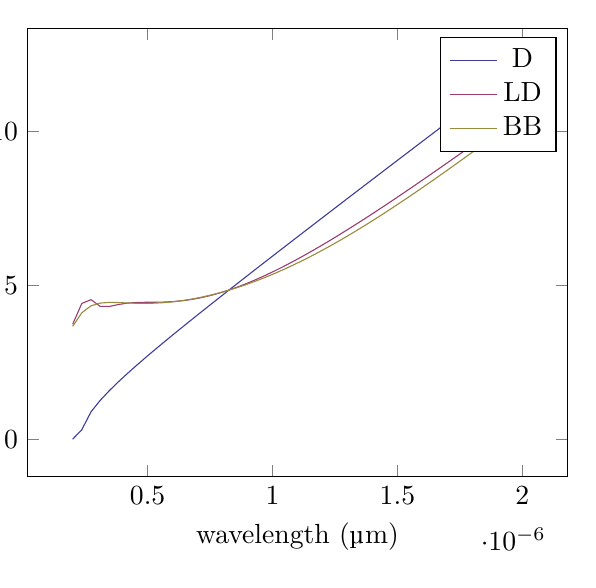
\begin{tikzpicture}[baseline,trim axis left]
			\begin{axis}[xlabel=wavelength (\si{\micro\meter}),ylabel=refractive index $n''$]
				\addplot[color=colora] coordinates {
						(2e-07, 0.005965630676535387)
						(2.3673469387755102e-07, 0.3145218480026841)
						(2.7346938775510205e-07, 0.8945915504579575)
						(3.1020408163265303e-07, 1.2661147295416986)
						(3.4693877551020406e-07, 1.5833005173347743)
						(3.836734693877551e-07, 1.8739410379205028)
						(4.2040816326530607e-07, 2.1488316557038036)
						(4.571428571428571e-07, 2.413357884801075)
						(4.938775510204081e-07, 2.6705990532454793)
						(5.306122448979591e-07, 2.922477320571435)
						(5.673469387755102e-07, 3.1702690252917565)
						(6.040816326530612e-07, 3.41486173083335)
						(6.408163265306121e-07, 3.656895255804831)
						(6.775510204081632e-07, 3.89684435489769)
						(7.142857142857142e-07, 4.135069786537969)
						(7.510204081632653e-07, 4.371851214337039)
						(7.877551020408163e-07, 4.607409157939915)
						(8.244897959183672e-07, 4.841920075287182)
						(8.612244897959183e-07, 5.075526989588498)
						(8.979591836734693e-07, 5.308347142032221)
						(9.346938775510204e-07, 5.54047760875608)
						(9.714285714285713e-07, 5.77199949364027)
						(1.0081632653061223e-06, 6.002981105305285)
						(1.0448979591836734e-06, 6.233480396996846)
						(1.0816326530612245e-06, 6.463546863247082)
						(1.1183673469387754e-06, 6.693223030571779)
						(1.1551020408163265e-06, 6.922545640911777)
						(1.1918367346938776e-06, 7.151546599822202)
						(1.2285714285714284e-06, 7.380253742621748)
						(1.2653061224489795e-06, 7.608691458298924)
						(1.3020408163265306e-06, 7.836881201267663)
						(1.3387755102040815e-06, 8.064841913958674)
						(1.3755102040816325e-06, 8.292590377970626)
						(1.4122448979591836e-06, 8.520141507567669)
						(1.4489795918367345e-06, 8.74750859633462)
						(1.4857142857142856e-06, 8.974703525532794)
						(1.5224489795918367e-06, 9.201736940955321)
						(1.5591836734693875e-06, 9.428618403729072)
						(1.5959183673469386e-06, 9.655356519454958)
						(1.6326530612244897e-06, 9.881959049248435)
						(1.6693877551020408e-06, 10.108433005585294)
						(1.7061224489795917e-06, 10.334784735334784)
						(1.7428571428571427e-06, 10.56101999194291)
						(1.7795918367346938e-06, 10.787143998391274)
						(1.8163265306122447e-06, 11.013161502283292)
						(1.8530612244897958e-06, 11.23907682418716)
						(1.8897959183673469e-06, 11.464893900182746)
						(1.9265306122448977e-06, 11.690616319410163)
						(1.963265306122449e-06, 11.916247357294232)
						(2e-06, 12.141790005016778)
					};
				\addlegendentry{D}
				\addplot[color=colorb] coordinates {
						(2e-07, 3.738034351582445)
						(2.3673469387755102e-07, 4.415954394360031)
						(2.7346938775510205e-07, 4.538183394846)
						(3.1020408163265303e-07, 4.320218714707598)
						(3.4693877551020406e-07, 4.317371587314897)
						(3.836734693877551e-07, 4.381449166256491)
						(4.2040816326530607e-07, 4.42743428874805)
						(4.571428571428571e-07, 4.447832095058005)
						(4.938775510204081e-07, 4.453232440283048)
						(5.306122448979591e-07, 4.454908827252396)
						(5.673469387755102e-07, 4.461085349160169)
						(6.040816326530612e-07, 4.476874449432579)
						(6.408163265306121e-07, 4.505046275574356)
						(6.775510204081632e-07, 4.54680917151326)
						(7.142857142857142e-07, 4.602403479418382)
						(7.510204081632653e-07, 4.671504511668752)
						(7.877551020408163e-07, 4.7534793116537495)
						(8.244897959183672e-07, 4.847543412940123)
						(8.612244897959183e-07, 4.952853246203722)
						(8.979591836734693e-07, 5.068558749955682)
						(9.346938775510204e-07, 5.193832130255906)
						(9.714285714285713e-07, 5.327882741459239)
						(1.0081632653061223e-06, 5.469964140654265)
						(1.0448979591836734e-06, 5.619376880191999)
						(1.0816326530612245e-06, 5.775469062335773)
						(1.1183673469387754e-06, 5.937635751510996)
						(1.1551020408163265e-06, 6.10531779946385)
						(1.1918367346938776e-06, 6.2780003407004745)
						(1.2285714285714284e-06, 6.455211064655143)
						(1.2653061224489795e-06, 6.636518305344469)
						(1.3020408163265306e-06, 6.821528969288432)
						(1.3387755102040815e-06, 7.009886323762714)
						(1.3755102040816325e-06, 7.20126767574952)
						(1.4122448979591836e-06, 7.395381979823209)
						(1.4489795918367345e-06, 7.591967417496154)
						(1.4857142857142856e-06, 7.790788990631591)
						(1.5224489795918367e-06, 7.991636168061834)
						(1.5591836734693875e-06, 8.194320618679379)
						(1.5959183673469386e-06, 8.398674057169142)
						(1.6326530612244897e-06, 8.604546221194374)
						(1.6693877551020408e-06, 8.811802991929017)
						(1.7061224489795917e-06, 9.02032466376667)
						(1.7428571428571427e-06, 9.230004364029686)
						(1.7795918367346938e-06, 9.440746619588815)
						(1.8163265306122447e-06, 9.65246606441707)
						(1.8530612244897958e-06, 9.865086280115857)
						(1.8897959183673469e-06, 10.078538760216844)
						(1.9265306122448977e-06, 10.292761988427952)
						(1.963265306122449e-06, 10.507700620815497)
						(2e-06, 10.723304762074587)
					};
				\addlegendentry{LD}
				\addplot[color=colorc] coordinates {
						(2e-07, 3.670010783409968)
						(2.3673469387755102e-07, 4.112324717336318)
						(2.7346938775510205e-07, 4.337439030548837)
						(3.1020408163265303e-07, 4.427636144475473)
						(3.4693877551020406e-07, 4.449809379072485)
						(3.836734693877551e-07, 4.443746535570925)
						(4.2040816326530607e-07, 4.43037324293511)
						(4.571428571428571e-07, 4.420021289722444)
						(4.938775510204081e-07, 4.41750669587497)
						(5.306122448979591e-07, 4.424864519229201)
						(5.673469387755102e-07, 4.442760529151114)
						(6.040816326530612e-07, 4.471210530116112)
						(6.408163265306121e-07, 4.5099445671983585)
						(6.775510204081632e-07, 4.558588943745782)
						(7.142857142857142e-07, 4.616754184405111)
						(7.510204081632653e-07, 4.684074188070827)
						(7.877551020408163e-07, 4.760220072904161)
						(8.244897959183672e-07, 4.844901077455748)
						(8.612244897959183e-07, 4.937859107424884)
						(8.979591836734693e-07, 5.038860492972576)
						(9.346938775510204e-07, 5.147686924996174)
						(9.714285714285713e-07, 5.264126689316893)
						(1.0081632653061223e-06, 5.387966857314872)
						(1.0448979591836734e-06, 5.51898682883406)
						(1.0816326530612245e-06, 5.656953455622987)
						(1.1183673469387754e-06, 5.801617847974093)
						(1.1551020408163265e-06, 5.952713859050278)
						(1.1918367346938776e-06, 6.1099581431311885)
						(1.2285714285714284e-06, 6.273051597701988)
						(1.2653061224489795e-06, 6.441681931105196)
						(1.3020408163265306e-06, 6.615527053631178)
						(1.3387755102040815e-06, 6.794258974050888)
						(1.3755102040816325e-06, 6.977547895383781)
						(1.4122448979591836e-06, 7.165066238966159)
						(1.4489795918367345e-06, 7.356492377686347)
						(1.4857142857142856e-06, 7.551513919446218)
						(1.5224489795918367e-06, 7.74983044275263)
						(1.5591836734693875e-06, 7.951155641651129)
						(1.5959183673469386e-06, 8.155218882945556)
						(1.6326530612244897e-06, 8.361766212933938)
						(1.6693877551020408e-06, 8.570560873688446)
						(1.7061224489795917e-06, 8.781383401445014)
						(1.7428571428571427e-06, 8.99403138388209)
						(1.7795918367346938e-06, 9.208318951123031)
						(1.8163265306122447e-06, 9.424076069247288)
						(1.8530612244897958e-06, 9.641147696689929)
						(1.8897959183673469e-06, 9.859392854508227)
						(1.9265306122448977e-06, 10.078683652070852)
						(1.963265306122449e-06, 10.298904300912687)
						(2e-06, 10.51995014165689)
					};
				\addlegendentry{BB}
			\end{axis}
		\end{tikzpicture}%
		\\
	\end{tabular}
	\caption{Complex permittivity $\epsilon = \epsilon' + \mi \epsilon''$ and refractive index $n = n' + \mi n''$ for Be based on the Drude (D), Lorentz-Drude (LD), and Brendel-Bormann (BB) models.}
\end{figure}
\clearpage
\newpage
\subsection{Pd}
\begin{figure}[h!]
	\centering
	\begin{tabular}{l}
		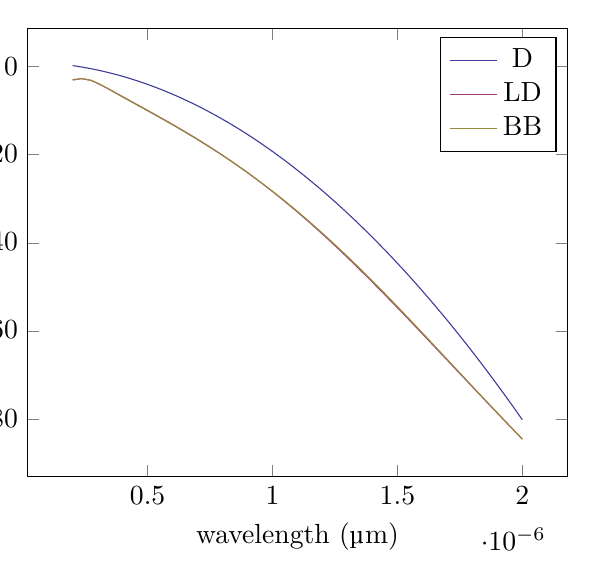
\begin{tikzpicture}[baseline,trim axis left]
			\begin{axis}[xlabel=wavelength (\si{\micro\meter}),ylabel=permittivity $\epsilon'$]
				\addplot[color=colora] coordinates {
						(2e-07, 0.18871572059628983)
						(2.3673469387755102e-07, -0.13667575717882485)
						(2.7346938775510205e-07, -0.5168054376999838)
						(3.1020408163265303e-07, -0.9516730646902258)
						(3.4693877551020406e-07, -1.4412783449699353)
						(3.836734693877551e-07, -1.985620948457333)
						(4.2040816326530607e-07, -2.584700508169036)
						(4.571428571428571e-07, -3.2385166202206737)
						(4.938775510204081e-07, -3.9470688438275667)
						(5.306122448979591e-07, -4.710356701305475)
						(5.673469387755102e-07, -5.528379678071402)
						(6.040816326530612e-07, -6.401137222644454)
						(6.408163265306121e-07, -7.32862874664678)
						(6.775510204081632e-07, -8.310853624804558)
						(7.142857142857142e-07, -9.347811194949053)
						(7.510204081632653e-07, -10.439500758017722)
						(7.877551020408163e-07, -11.585921578055403)
						(8.244897959183672e-07, -12.787072882215556)
						(8.612244897959183e-07, -14.042953860761571)
						(8.979591836734693e-07, -15.353563667068094)
						(9.346938775510204e-07, -16.718901417622515)
						(9.714285714285713e-07, -18.138966192026395)
						(1.0081632653061223e-06, -19.613757032997082)
						(1.0448979591836734e-06, -21.14327294636925)
						(1.0816326530612245e-06, -22.727512901096663)
						(1.1183673469387754e-06, -24.366475829253794)
						(1.1551020408163265e-06, -26.06016062603777)
						(1.1918367346938776e-06, -27.80856614977011)
						(1.2285714285714284e-06, -29.611691221898695)
						(1.2653061224489795e-06, -31.469534626999774)
						(1.3020408163265306e-06, -33.38209511278)
						(1.3387755102040815e-06, -35.34937139007851)
						(1.3755102040816325e-06, -37.37136213286914)
						(1.4122448979591836e-06, -39.44806597826261)
						(1.4489795918367345e-06, -41.579481526508886)
						(1.4857142857142856e-06, -43.76560734099948)
						(1.5224489795918367e-06, -46.0064419482699)
						(1.5591836734693875e-06, -48.301983838002144)
						(1.5959183673469386e-06, -50.652231463027185)
						(1.6326530612244897e-06, -53.05718323932767)
						(1.6693877551020408e-06, -55.51683754604046)
						(1.7061224489795917e-06, -58.03119272545953)
						(1.7428571428571427e-06, -60.600247083038596)
						(1.7795918367346938e-06, -63.22399888739412)
						(1.8163265306122447e-06, -65.90244637030803)
						(1.8530612244897958e-06, -68.63558772673096)
						(1.8897959183673469e-06, -71.42342111478504)
						(1.9265306122448977e-06, -74.26594465576716)
						(1.963265306122449e-06, -77.16315643415207)
						(2e-06, -80.11505449759562)
					};
				\addlegendentry{D}
				\addplot[color=colorb] coordinates {
						(2e-07, -3.0055563348908243)
						(2.3673469387755102e-07, -2.7865004217398104)
						(2.7346938775510205e-07, -3.1593757688682578)
						(3.1020408163265303e-07, -4.096873948227486)
						(3.4693877551020406e-07, -5.202690429238098)
						(3.836734693877551e-07, -6.3454267091644)
						(4.2040816326530607e-07, -7.4923529671790305)
						(4.571428571428571e-07, -8.638311294772887)
						(4.938775510204081e-07, -9.78623018191674)
						(5.306122448979591e-07, -10.941456571711557)
						(5.673469387755102e-07, -12.109879737471749)
						(6.040816326530612e-07, -13.297233812183446)
						(6.408163265306121e-07, -14.50882150580966)
						(6.775510204081632e-07, -15.749408568574042)
						(7.142857142857142e-07, -17.023194114309568)
						(7.510204081632653e-07, -18.33381601547431)
						(7.877551020408163e-07, -19.684371989661265)
						(8.244897959183672e-07, -21.0774465761932)
						(8.612244897959183e-07, -22.515138950792213)
						(8.979591836734693e-07, -23.9990890621107)
						(9.346938775510204e-07, -25.53050099075924)
						(9.714285714285713e-07, -27.110163240945205)
						(1.0081632653061223e-06, -28.73846613984083)
						(1.0448979591836734e-06, -30.41541678528162)
						(1.0816326530612245e-06, -32.14065213183831)
						(1.1183673469387754e-06, -33.91345088766395)
						(1.1551020408163265e-06, -35.732744938285606)
						(1.1918367346938776e-06, -37.597131034564605)
						(1.2285714285714284e-06, -39.50488348830155)
						(1.2653061224489795e-06, -41.45396861317147)
						(1.3020408163265306e-06, -43.442061630277365)
						(1.3387755102040815e-06, -45.46656672391988)
						(1.3755102040816325e-06, -47.524640880275754)
						(1.4122448979591836e-06, -49.61322206512419)
						(1.4489795918367345e-06, -51.72906219225594)
						(1.4857142857142856e-06, -53.868765198222064)
						(1.5224489795918367e-06, -56.028830369527206)
						(1.5591836734693875e-06, -58.20570086521127)
						(1.5959183673469386e-06, -60.39581714362258)
						(1.6326530612244897e-06, -62.59567474284169)
						(1.6693877551020408e-06, -64.80188558888875)
						(1.7061224489795917e-06, -67.01124172721764)
						(1.7428571428571427e-06, -69.22078010685205)
						(1.7795918367346938e-06, -71.42784681098534)
						(1.8163265306122447e-06, -73.63015894221354)
						(1.8530612244897958e-06, -75.82586225363636)
						(1.8897959183673469e-06, -78.01358258536445)
						(1.9265306122448977e-06, -80.19246923180305)
						(1.963265306122449e-06, -82.36222853466778)
						(2e-06, -84.52314626882317)
					};
				\addlegendentry{LD}
				\addplot[color=colorc] coordinates {
						(2e-07, -3.1039254576280597)
						(2.3673469387755102e-07, -2.7485197943844)
						(2.7346938775510205e-07, -3.154593245328339)
						(3.1020408163265303e-07, -4.100200351809187)
						(3.4693877551020406e-07, -5.237804207460961)
						(3.836734693877551e-07, -6.409467072846786)
						(4.2040816326530607e-07, -7.571125832043443)
						(4.571428571428571e-07, -8.720772106358009)
						(4.938775510204081e-07, -9.867133495129135)
						(5.306122448979591e-07, -11.019475797323917)
						(5.673469387755102e-07, -12.185318966784005)
						(6.040816326530612e-07, -13.3705090403609)
						(6.408163265306121e-07, -14.57973072142095)
						(6.775510204081632e-07, -15.816929636174423)
						(7.142857142857142e-07, -17.085566211932818)
						(7.510204081632653e-07, -18.388740936741343)
						(7.877551020408163e-07, -19.72924277915066)
						(8.244897959183672e-07, -21.109558688498588)
						(8.612244897959183e-07, -22.5318669105135)
						(8.979591836734693e-07, -23.998025985165647)
						(9.346938775510204e-07, -25.509564710390023)
						(9.714285714285713e-07, -27.067674800665316)
						(1.0081632653061223e-06, -28.673206275889328)
						(1.0448979591836734e-06, -30.326664967499696)
						(1.0816326530612245e-06, -32.028211421361824)
						(1.1183673469387754e-06, -33.77766062291301)
						(1.1551020408163265e-06, -35.57448221586672)
						(1.1918367346938776e-06, -37.41780115526803)
						(1.2285714285714284e-06, -39.30639899452541)
						(1.2653061224489795e-06, -41.238716240748616)
						(1.3020408163265306e-06, -43.21285641875836)
						(1.3387755102040815e-06, -45.22659265936949)
						(1.3755102040816325e-06, -47.277377768825865)
						(1.4122448979591836e-06, -49.36235883777757)
						(1.4489795918367345e-06, -51.4783975009718)
						(1.4857142857142856e-06, -53.622096951036525)
						(1.5224489795918367e-06, -55.78983672763454)
						(1.5591836734693875e-06, -57.97781613290894)
						(1.5959183673469386e-06, -60.182106853701065)
						(1.6326530612244897e-06, -62.398714993712545)
						(1.6693877551020408e-06, -64.62365223611302)
						(1.7061224489795917e-06, -66.8530152819655)
						(1.7428571428571427e-06, -69.08307206895216)
						(1.7795918367346938e-06, -71.31035260957707)
						(1.8163265306122447e-06, -73.53174165295016)
						(1.8530612244897958e-06, -75.74456983335455)
						(1.8897959183673469e-06, -77.94669958854163)
						(1.9265306122448977e-06, -80.13660197132819)
						(1.963265306122449e-06, -82.31342058403344)
						(2e-06, -84.47701925659831)
					};
				\addlegendentry{BB}
			\end{axis}
		\end{tikzpicture}%
		\\
		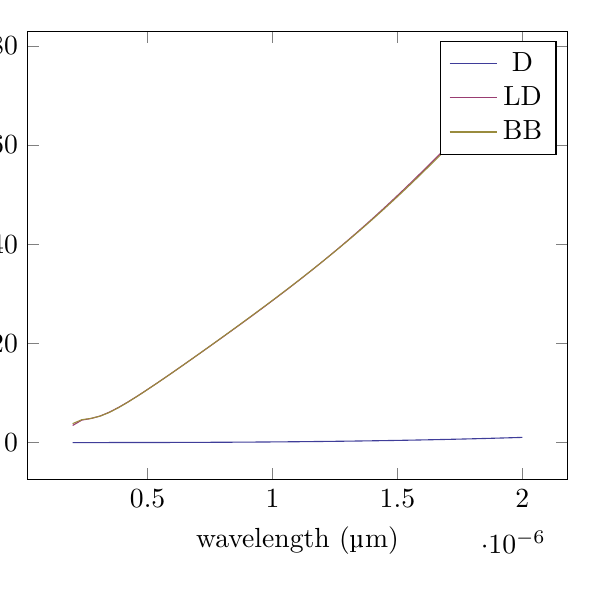
\begin{tikzpicture}[baseline,trim axis left]
			\begin{axis}[xlabel=wavelength (\si{\micro\meter}),ylabel=permittivity $\epsilon''$]
				\addplot[color=colora] coordinates {
						(2e-07, 0.001046951840193811)
						(2.3673469387755102e-07, 0.0017362895647302485)
						(2.7346938775510205e-07, 0.0026764691606400697)
						(3.1020408163265303e-07, 0.0039064136128966545)
						(3.4693877551020406e-07, 0.005465045580883607)
						(3.836734693877551e-07, 0.007391287354661116)
						(4.2040816326530607e-07, 0.009724060811233197)
						(4.571428571428571e-07, 0.012502287370815898)
						(4.938775510204081e-07, 0.015764887953106595)
						(5.306122448979591e-07, 0.019550782933554466)
						(5.673469387755102e-07, 0.023898892099632255)
						(6.040816326530612e-07, 0.028848134607109395)
						(6.408163265306121e-07, 0.03443742893632666)
						(6.775510204081632e-07, 0.04070569284847236)
						(7.142857142857142e-07, 0.04769184334186036)
						(7.510204081632653e-07, 0.055434796608209644)
						(7.877551020408163e-07, 0.06397346798892607)
						(8.244897959183672e-07, 0.073346771931386)
						(8.612244897959183e-07, 0.08359362194522207)
						(8.979591836734693e-07, 0.09475293055861089)
						(9.346938775510204e-07, 0.10686360927456372)
						(9.714285714285713e-07, 0.11996456852721873)
						(1.0081632653061223e-06, 0.13409471763813674)
						(1.0448979591836734e-06, 0.1492929647725984)
						(1.0816326530612245e-06, 0.16559821689590556)
						(1.1183673469387754e-06, 0.18304937972968352)
						(1.1551020408163265e-06, 0.20168535770818882)
						(1.1918367346938776e-06, 0.22154505393461746)
						(1.2285714285714284e-06, 0.24266737013741752)
						(1.2653061224489795e-06, 0.2650912066266056)
						(1.3020408163265306e-06, 0.2888554622500855)
						(1.3387755102040815e-06, 0.31399903434997034)
						(1.3755102040816325e-06, 0.34056081871890964)
						(1.4122448979591836e-06, 0.368579709556418)
						(1.4489795918367345e-06, 0.39809459942520914)
						(1.4857142857142856e-06, 0.4291443792075335)
						(1.5224489795918367e-06, 0.4617679380615192)
						(1.5591836734693875e-06, 0.49600416337751774)
						(1.5959183673469386e-06, 0.5318919407344528)
						(1.6326530612244897e-06, 0.5694701538561758)
						(1.6693877551020408e-06, 0.6087776845678214)
						(1.7061224489795917e-06, 0.6498534127521731)
						(1.7428571428571427e-06, 0.6927362163060283)
						(1.7795918367346938e-06, 0.7374649710965722)
						(1.8163265306122447e-06, 0.7840785509177518)
						(1.8530612244897958e-06, 0.8326158274466616)
						(1.8897959183673469e-06, 0.8831156701999259)
						(1.9265306122448977e-06, 0.9356169464900925)
						(1.963265306122449e-06, 0.9901585213820312)
						(2e-06, 1.046779257649333)
					};
				\addlegendentry{D}
				\addplot[color=colorb] coordinates {
						(2e-07, 3.4451565445776424)
						(2.3673469387755102e-07, 4.534790530683119)
						(2.7346938775510205e-07, 4.851848932640109)
						(3.1020408163265303e-07, 5.354911220679058)
						(3.4693877551020406e-07, 6.13167648233587)
						(3.836734693877551e-07, 7.089876420374707)
						(4.2040816326530607e-07, 8.163301384974318)
						(4.571428571428571e-07, 9.312122369135027)
						(4.938775510204081e-07, 10.51167362779882)
						(5.306122448979591e-07, 11.746016094597861)
						(5.673469387755102e-07, 13.00457630241439)
						(6.040816326530612e-07, 14.280297866662622)
						(6.408163265306121e-07, 15.568546641008064)
						(6.775510204081632e-07, 16.866417242156412)
						(7.142857142857142e-07, 18.17226975833794)
						(7.510204081632653e-07, 19.485407427712794)
						(7.877551020408163e-07, 20.80584524345563)
						(8.244897959183672e-07, 22.134139464655753)
						(8.612244897959183e-07, 23.471258984432513)
						(8.979591836734693e-07, 24.818485923392547)
						(9.346938775510204e-07, 26.177336786418977)
						(9.714285714285713e-07, 27.5494980928467)
						(1.0081632653061223e-06, 28.936772119290847)
						(1.0448979591836734e-06, 30.34102959267303)
						(1.0816326530612245e-06, 31.76416702382991)
						(1.1183673469387754e-06, 33.20806699537611)
						(1.1551020408163265e-06, 34.674560186628305)
						(1.1918367346938776e-06, 36.16538828395711)
						(1.2285714285714284e-06, 37.68216722153543)
						(1.2653061224489795e-06, 39.226350448924094)
						(1.3020408163265306e-06, 40.79919214446362)
						(1.3387755102040815e-06, 42.401710497489624)
						(1.3755102040816325e-06, 44.03465137390138)
						(1.4122448979591836e-06, 45.69845286078526)
						(1.4489795918367345e-06, 47.39321135558986)
						(1.4857142857142856e-06, 49.11865001992181)
						(1.5224489795918367e-06, 50.87409055113989)
						(1.5591836734693875e-06, 52.65842932843927)
						(1.5959183673469386e-06, 54.470119054657545)
						(1.6326530612244897e-06, 56.307157030802614)
						(1.6693877551020408e-06, 58.16708115808577)
						(1.7061224489795917e-06, 60.04697465457253)
						(1.7428571428571427e-06, 61.9434802959348)
						(1.7795918367346938e-06, 63.85282474184587)
						(1.8163265306122447e-06, 65.77085319607164)
						(1.8530612244897958e-06, 67.6930742797882)
						(1.8897959183673469e-06, 69.61471459044158)
						(1.9265306122448977e-06, 71.53078199419221)
						(1.963265306122449e-06, 73.43613628433712)
						(2e-06, 75.32556545892535)
					};
				\addlegendentry{LD}
				\addplot[color=colorc] coordinates {
						(2e-07, 3.8248725466092615)
						(2.3673469387755102e-07, 4.614148269407245)
						(2.7346938775510205e-07, 4.877271848504206)
						(3.1020408163265303e-07, 5.334141382657037)
						(3.4693877551020406e-07, 6.083477036817123)
						(3.836734693877551e-07, 7.041510750027717)
						(4.2040816326530607e-07, 8.126140437027647)
						(4.571428571428571e-07, 9.286237043731306)
						(4.938775510204081e-07, 10.493581642387298)
						(5.306122448979591e-07, 11.732777683222585)
						(5.673469387755102e-07, 12.99496531486842)
						(6.040816326530612e-07, 14.274589325633448)
						(6.408163265306121e-07, 15.5678863519115)
						(6.775510204081632e-07, 16.872211434737345)
						(7.142857142857142e-07, 18.18573766285443)
						(7.510204081632653e-07, 19.507307836059493)
						(7.877551020408163e-07, 20.836342251948064)
						(8.244897959183672e-07, 22.172765113672426)
						(8.612244897959183e-07, 23.516937135682483)
						(8.979591836734693e-07, 24.869591570112945)
						(9.346938775510204e-07, 26.231773881926433)
						(9.714285714285713e-07, 27.604785730637627)
						(1.0081632653061223e-06, 28.990133530935857)
						(1.0448979591836734e-06, 30.38948135930348)
						(1.0816326530612245e-06, 31.80460757957497)
						(1.1183673469387754e-06, 33.237364321455075)
						(1.1551020408163265e-06, 34.689638842431016)
						(1.1918367346938776e-06, 36.16331580167299)
						(1.2285714285714284e-06, 37.660239545234)
						(1.2653061224489795e-06, 39.182175624993334)
						(1.3020408163265306e-06, 40.73077093766405)
						(1.3387755102040815e-06, 42.3075120694059)
						(1.3755102040816325e-06, 43.91368166450544)
						(1.4122448979591836e-06, 45.5503129029401)
						(1.4489795918367345e-06, 47.218142470389225)
						(1.4857142857142856e-06, 48.91756273156618)
						(1.5224489795918367e-06, 50.64857416528425)
						(1.5591836734693875e-06, 52.41073947313413)
						(1.5959183673469386e-06, 54.203141111892954)
						(1.6326530612244897e-06, 56.02434429474228)
						(1.6693877551020408e-06, 57.872367724174254)
						(1.7061224489795917e-06, 59.74466442294804)
						(1.7428571428571427e-06, 61.63811498222032)
						(1.7795918367346938e-06, 63.54903531776776)
						(1.8163265306122447e-06, 65.4732005980488)
						(1.8530612244897958e-06, 67.40588638190027)
						(1.8897959183673469e-06, 69.34192720166878)
						(1.9265306122448977e-06, 71.27579189645688)
						(1.963265306122449e-06, 73.20167400892932)
						(2e-06, 75.11359459259634)
					};
				\addlegendentry{BB}
			\end{axis}
		\end{tikzpicture}%
		\\
		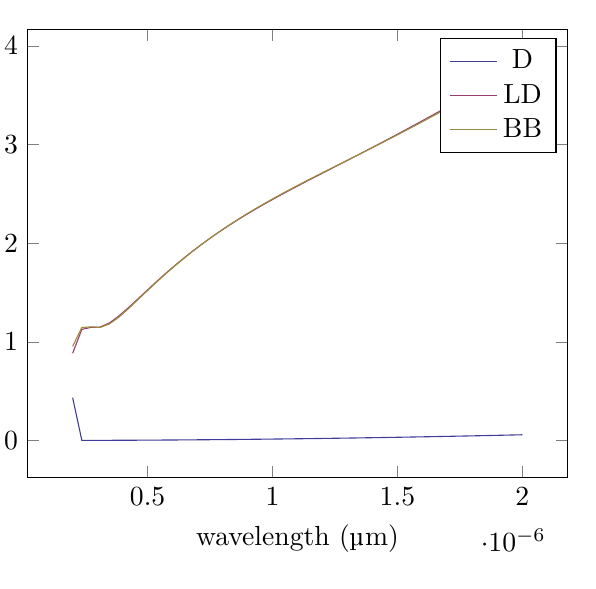
\begin{tikzpicture}[baseline,trim axis left]
			\begin{axis}[xlabel=wavelength (\si{\micro\meter}),ylabel=refractive index $n'$]
				\addplot[color=colora] coordinates {
						(2e-07, 0.43441589824465665)
						(2.3673469387755102e-07, 0.002348213900929988)
						(2.7346938775510205e-07, 0.0018615180630071288)
						(3.1020408163265303e-07, 0.002002181413915554)
						(3.4693877551020406e-07, 0.0022760881703017283)
						(3.836734693877551e-07, 0.0026226550083883323)
						(4.2040816326530607e-07, 0.0030242089058054394)
						(4.571428571428571e-07, 0.0034736463998292287)
						(4.938775510204081e-07, 0.003967552443988951)
						(5.306122448979591e-07, 0.004504082377143558)
						(5.673469387755102e-07, 0.005082154075154132)
						(6.040816326530612e-07, 0.005701092256106863)
						(6.408163265306121e-07, 0.006360454713163206)
						(6.775510204081632e-07, 0.007059940429980552)
						(7.142857142857142e-07, 0.007799337860145223)
						(7.510204081632653e-07, 0.00857849429867838)
						(7.877551020408163e-07, 0.009397296966275039)
						(8.244897959183672e-07, 0.010255660904587917)
						(8.612244897959183e-07, 0.011153520992141296)
						(8.979591836734693e-07, 0.0120908265377891)
						(9.346938775510204e-07, 0.013067537534248427)
						(9.714285714285713e-07, 0.014083622009494309)
						(1.0081632653061223e-06, 0.01513905411902669)
						(1.0448979591836734e-06, 0.016233812750746895)
						(1.0816326530612245e-06, 0.01736788048868481)
						(1.1183673469387754e-06, 0.018541242833285163)
						(1.1551020408163265e-06, 0.019753887608140643)
						(1.1918367346938776e-06, 0.021005804502620372)
						(1.2285714285714284e-06, 0.022296984717021573)
						(1.2653061224489795e-06, 0.023627420682969268)
						(1.3020408163265306e-06, 0.024997105842991002)
						(1.3387755102040815e-06, 0.02640603447378702)
						(1.3755102040816325e-06, 0.027854201545099735)
						(1.4122448979591836e-06, 0.029341602603976846)
						(1.4489795918367345e-06, 0.030868233682141626)
						(1.4857142857142856e-06, 0.03243409121845497)
						(1.5224489795918367e-06, 0.03403917199628868)
						(1.5591836734693875e-06, 0.03568347309040205)
						(1.5959183673469386e-06, 0.03736699182384533)
						(1.6326530612244897e-06, 0.03908972573078113)
						(1.6693877551020408e-06, 0.04085167252595867)
						(1.7061224489795917e-06, 0.04265283007859317)
						(1.7428571428571427e-06, 0.044493196390299354)
						(1.7795918367346938e-06, 0.0463727695761249)
						(1.8163265306122447e-06, 0.04829154784867612)
						(1.8530612244897958e-06, 0.05024952950409649)
						(1.8897959183673469e-06, 0.052246712910468285)
						(1.9265306122448977e-06, 0.05428309649703595)
						(1.963265306122449e-06, 0.05635867874597363)
						(2e-06, 0.0584734581841087)
					};
				\addlegendentry{D}
				\addplot[color=colorb] coordinates {
						(2e-07, 0.8849762295493965)
						(2.3673469387755102e-07, 1.1260529547208076)
						(2.7346938775510205e-07, 1.1468327994085088)
						(3.1020408163265303e-07, 1.1501061737550689)
						(3.4693877551020406e-07, 1.1913841281181594)
						(3.836734693877551e-07, 1.2588367880941622)
						(4.2040816326530607e-07, 1.3394080791368148)
						(4.571428571428571e-07, 1.4253949229670655)
						(4.938775510204081e-07, 1.5125671847169588)
						(5.306122448979591e-07, 1.5986077643589203)
						(5.673469387755102e-07, 1.682258570093314)
						(6.040816326530612e-07, 1.762868639872507)
						(6.408163265306121e-07, 1.8401475782032728)
						(6.775510204081632e-07, 1.9140250976408415)
						(7.142857142857142e-07, 1.9845676167269295)
						(7.510204081632653e-07, 2.051926913180707)
						(7.877551020408163e-07, 2.1163075290587714)
						(8.244897959183672e-07, 2.177945533687446)
						(8.612244897959183e-07, 2.2370943671122037)
						(8.979591836734693e-07, 2.2940152022072815)
						(9.346938775510204e-07, 2.348970245123283)
						(9.714285714285713e-07, 2.402217975021581)
						(1.0081632653061223e-06, 2.4540096786414227)
						(1.0448979591836734e-06, 2.5045868571069088)
						(1.0816326530612245e-06, 2.554179224238948)
						(1.1183673469387754e-06, 2.6030031081016505)
						(1.1551020408163265e-06, 2.651260128893246)
						(1.1918367346938776e-06, 2.6991360678301217)
						(1.2285714285714284e-06, 2.7467998704240397)
						(1.2653061224489795e-06, 2.7944027480182214)
						(1.3020408163265306e-06, 2.84207735652876)
						(1.3387755102040815e-06, 2.889937042904319)
						(1.3755102040816325e-06, 2.9380751590580387)
						(1.4122448979591836e-06, 2.9865644506677804)
						(1.4489795918367345e-06, 3.0354565346888176)
						(1.4857142857142856e-06, 3.0847814848537145)
						(1.5224489795918367e-06, 3.134547548861799)
						(1.5591836734693875e-06, 3.1847410242871668)
						(1.5959183673469386e-06, 3.2353263222888953)
						(1.6326530612244897e-06, 3.286246248784994)
						(1.6693877551020408e-06, 3.3374225316469697)
						(1.7061224489795917e-06, 3.388756619515267)
						(1.7428571428571427e-06, 3.440130772926049)
						(1.7795918367346938e-06, 3.491409461576394)
						(1.8163265306122447e-06, 3.5424410728624003)
						(1.8530612244897958e-06, 3.593059926569126)
						(1.8897959183673469e-06, 3.643088579184834)
						(1.9265306122448977e-06, 3.6923403893017395)
						(1.963265306122449e-06, 3.740622303607306)
						(2e-06, 3.7877378117866263)
					};
				\addlegendentry{LD}
				\addplot[color=colorc] coordinates {
						(2e-07, 0.9544435688172067)
						(2.3673469387755102e-07, 1.1450346654121213)
						(2.7346938775510205e-07, 1.1519452157822516)
						(3.1020408163265303e-07, 1.146233999148603)
						(3.4693877551020406e-07, 1.1810701386033287)
						(3.836734693877551e-07, 1.2474583992334976)
						(4.2040816326530607e-07, 1.3295588580171454)
						(4.571428571428571e-07, 1.4174594660492221)
						(4.938775510204081e-07, 1.5061339762566512)
						(5.306122448979591e-07, 1.593220222988771)
						(5.673469387755102e-07, 1.6776520204054945)
						(6.040816326530612e-07, 1.758973838067824)
						(6.408163265306121e-07, 1.8370223078364343)
						(6.775510204081632e-07, 1.911782550289542)
						(7.142857142857142e-07, 1.9833231707837364)
						(7.510204081632653e-07, 2.051765417506407)
						(7.877551020408163e-07, 2.117266862360874)
						(8.244897959183672e-07, 2.1800112806018563)
						(8.612244897959183e-07, 2.240201341084623)
						(8.979591836734693e-07, 2.2980527812073053)
						(9.346938775510204e-07, 2.3537895560875706)
						(9.714285714285713e-07, 2.4076397490348933)
						(1.0081632653061223e-06, 2.4598321255672166)
						(1.0448979591836734e-06, 2.510593237152751)
						(1.0816326530612245e-06, 2.560144984691764)
						(1.1183673469387754e-06, 2.608702553390426)
						(1.1551020408163265e-06, 2.6564726350109202)
						(1.1918367346938776e-06, 2.7036518608568167)
						(1.2285714285714284e-06, 2.750425378411863)
						(1.2653061224489795e-06, 2.7969655154111206)
						(1.3020408163265306e-06, 2.843430486696292)
						(1.3387755102040815e-06, 2.889963111199565)
						(1.3755102040816325e-06, 2.9366895187241076)
						(1.4122448979591836e-06, 2.983717838853577)
						(1.4489795918367345e-06, 3.031136877338398)
						(1.4857142857142856e-06, 3.079014798602999)
						(1.5224489795918367e-06, 3.127397846381145)
						(1.5591836734693875e-06, 3.176309147506662)
						(1.5959183673469386e-06, 3.225747655934631)
						(1.6326530612244897e-06, 3.275687304293819)
						(1.6693877551020408e-06, 3.326076437645466)
						(1.7061224489795917e-06, 3.376837607519929)
						(1.7428571428571427e-06, 3.427867802626555)
						(1.7795918367346938e-06, 3.4790391849903104)
						(1.8163265306122447e-06, 3.530200386154576)
						(1.8530612244897958e-06, 3.581178397562165)
						(1.8897959183673469e-06, 3.631781063037752)
						(1.9265306122448977e-06, 3.6818001509302127)
						(1.963265306122449e-06, 3.731014951083681)
						(2e-06, 3.7791963100123542)
					};
				\addlegendentry{BB}
			\end{axis}
		\end{tikzpicture}%
		\\
		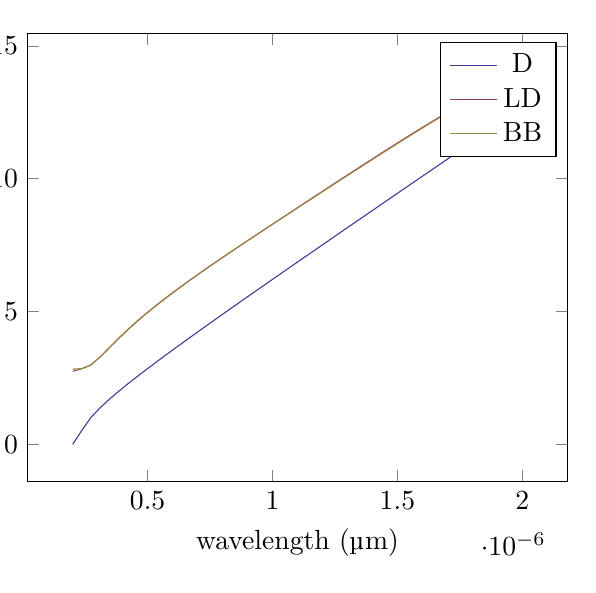
\begin{tikzpicture}[baseline,trim axis left]
			\begin{axis}[xlabel=wavelength (\si{\micro\meter}),ylabel=refractive index $n''$]
				\addplot[color=colora] coordinates {
						(2e-07, 0.0017041428473667192)
						(2.3673469387755102e-07, 0.5228408386638316)
						(2.7346938775510205e-07, 1.016669959179952)
						(3.1020408163265303e-07, 1.3796210156565754)
						(3.4693877551020406e-07, 1.6978124310696363)
						(3.836734693877551e-07, 1.9928009568326819)
						(4.2040816326530607e-07, 2.273635702573542)
						(4.571428571428571e-07, 2.5450063600863495)
						(4.938775510204081e-07, 2.80965641504436)
						(5.306122448979591e-07, 3.0693246775352834)
						(5.673469387755102e-07, 3.3251783429949877)
						(6.040816326530612e-07, 3.5780356971660767)
						(6.408163265306121e-07, 3.8284903557488397)
						(6.775510204081632e-07, 4.076985030034678)
						(7.142857142857142e-07, 4.323857542662595)
						(7.510204081632653e-07, 4.569370711286655)
						(7.877551020408163e-07, 4.81373241617057)
						(8.244897959183672e-07, 5.057109463081879)
						(8.612244897959183e-07, 5.2996373954813345)
						(8.979591836734693e-07, 5.5414275877529)
						(9.346938775510204e-07, 5.78257246874775)
						(9.714285714285713e-07, 6.02314943205551)
						(1.0081632653061223e-06, 6.263223806308809)
						(1.0448979591836734e-06, 6.502851141314197)
						(1.0816326530612245e-06, 6.742078988616098)
						(1.1183673469387754e-06, 6.980948303338107)
						(1.1551020408163265e-06, 7.219494558778115)
						(1.1918367346938776e-06, 7.45774864065462)
						(1.2285714285714284e-06, 7.695737570555036)
						(1.2653061224489795e-06, 7.933485095720279)
						(1.3020408163265306e-06, 8.171012173296589)
						(1.3387755102040815e-06, 8.408337370578698)
						(1.3755102040816325e-06, 8.645477197866274)
						(1.4122448979591836e-06, 8.882446386880812)
						(1.4489795918367345e-06, 9.119258124909015)
						(1.4857142857142856e-06, 9.355924252715244)
						(1.5224489795918367e-06, 9.592455432630386)
						(1.5591836734693875e-06, 9.828861291955842)
						(1.5959183673469386e-06, 10.065150545829422)
						(1.6326530612244897e-06, 10.301331102919212)
						(1.6693877551020408e-06, 10.537410156693023)
						(1.7061224489795917e-06, 10.773394264517869)
						(1.7428571428571427e-06, 11.009289416448604)
						(1.7795918367346938e-06, 11.245101095246078)
						(1.8163265306122447e-06, 11.480834328906733)
						(1.8530612244897958e-06, 11.716493736775208)
						(1.8897959183673469e-06, 11.952083570139141)
						(1.9265306122448977e-06, 12.187607748063806)
						(1.963265306122449e-06, 12.423069889107287)
						(2e-06, 12.658473339459828)
					};
				\addlegendentry{D}
				\addplot[color=colorb] coordinates {
						(2e-07, 2.7527220207490224)
						(2.3673469387755102e-07, 2.847629076468799)
						(2.7346938775510205e-07, 2.9915217661475957)
						(3.1020408163265303e-07, 3.29229954868539)
						(3.4693877551020406e-07, 3.639254475842536)
						(3.836734693877551e-07, 3.98248584886968)
						(4.2040816326530607e-07, 4.30960948802464)
						(4.571428571428571e-07, 4.619537202186637)
						(4.938775510204081e-07, 4.914079704318872)
						(5.306122448979591e-07, 5.195575686289284)
						(5.673469387755102e-07, 5.466237030009612)
						(6.040816326530612e-07, 5.7279908613106905)
						(6.408163265306121e-07, 5.982468489741844)
						(6.775510204081632e-07, 6.23103533017958)
						(7.142857142857142e-07, 6.474828606174958)
						(7.510204081632653e-07, 6.714792636040165)
						(7.877551020408163e-07, 6.951709077228722)
						(8.244897959183672e-07, 7.186222001010308)
						(8.612244897959183e-07, 7.418858424064631)
						(8.979591836734693e-07, 7.650045073078827)
						(9.346938775510204e-07, 7.880122106063304)
						(9.714285714285713e-07, 8.109354405926775)
						(1.0081632653061223e-06, 8.337940949983588)
						(1.0448979591836734e-06, 8.566022660497028)
						(1.0816326530612245e-06, 8.79368905993067)
						(1.1183673469387754e-06, 9.02098398939393)
						(1.1551020408163265e-06, 9.247910597464125)
						(1.1918367346938776e-06, 9.47443576654843)
						(1.2285714285714284e-06, 9.700494112823643)
						(1.2653061224489795e-06, 9.925991671495927)
						(1.3020408163265306e-06, 10.150809359925038)
						(1.3387755102040815e-06, 10.374806295625035)
						(1.3755102040816325e-06, 10.597823033109174)
						(1.4122448979591836e-06, 10.819684772036267)
						(1.4489795918367345e-06, 11.040204578379967)
						(1.4857142857142856e-06, 11.259186649800096)
						(1.5224489795918367e-06, 11.476429645634806)
						(1.5591836734693875e-06, 11.691730090708472)
						(1.5959183673469386e-06, 11.904885850382437)
						(1.6326530612244897e-06, 12.11569966204966)
						(1.6693877551020408e-06, 12.323982695836085)
						(1.7061224489795917e-06, 12.5295581050192)
						(1.7428571428571427e-06, 12.732264515135148)
						(1.7795918367346938e-06, 12.931959390546393)
						(1.8163265306122447e-06, 13.128522209061922)
						(1.8530612244897958e-06, 13.321857369717879)
						(1.8897959183673469e-06, 13.51189675664756)
						(1.9265306122448977e-06, 13.698601883569868)
						(1.963265306122449e-06, 13.881965549079295)
						(2e-06, 14.062012942652364)
					};
				\addlegendentry{LD}
				\addplot[color=colorc] coordinates {
						(2e-07, 2.8336859330859467)
						(2.3673469387755102e-07, 2.849429479520365)
						(2.7346938775510205e-07, 2.9938507061949355)
						(3.1020408163265303e-07, 3.2906086770120164)
						(3.4693877551020406e-07, 3.6421781614197424)
						(3.836734693877551e-07, 3.9913956282646263)
						(4.2040816326530607e-07, 4.321771069590637)
						(4.571428571428571e-07, 4.6324860375937575)
						(4.938775510204081e-07, 4.926575494106186)
						(5.306122448979591e-07, 5.207269241409418)
						(5.673469387755102e-07, 5.477195499223055)
						(6.040816326530612e-07, 5.738379214267379)
						(6.408163265306121e-07, 5.992392123502875)
						(6.775510204081632e-07, 6.24048750591907)
						(7.142857142857142e-07, 6.48369293099241)
						(7.510204081632653e-07, 6.722868772364456)
						(7.877551020408163e-07, 6.958744390420174)
						(8.244897959183672e-07, 7.191941027573841)
						(8.612244897959183e-07, 7.422987129062106)
						(8.979591836734693e-07, 7.65232939311688)
						(9.346938775510204e-07, 7.880341361227564)
						(9.714285714285713e-07, 8.107330505388086)
						(1.0081632653061223e-06, 8.333544307419487)
						(1.0448979591836734e-06, 8.55917558762955)
						(1.0816326530612245e-06, 8.784367224109454)
						(1.1183673469387754e-06, 9.009216351601147)
						(1.1551020408163265e-06, 9.23377810827492)
						(1.1918367346938776e-06, 9.458068993191217)
						(1.2285714285714284e-06, 9.682069898191962)
						(1.2653061224489795e-06, 9.90572888132394)
						(1.3020408163265306e-06, 10.128963752668115)
						(1.3387755102040815e-06, 10.351664546676902)
						(1.3755102040816325e-06, 10.57369595725259)
						(1.4122448979591836e-06, 10.794899812380905)
						(1.4489795918367345e-06, 11.015097663673489)
						(1.4857142857142856e-06, 11.234093562103958)
						(1.5224489795918367e-06, 11.45167708391954)
						(1.5591836734693875e-06, 11.667626659560497)
						(1.5959183673469386e-06, 11.881713242918197)
						(1.6326530612244897e-06, 12.093704338144228)
						(1.6693877551020408e-06, 12.30336837660105)
						(1.7061224489795917e-06, 12.510479408042396)
						(1.7428571428571427e-06, 12.714822038961927)
						(1.7795918367346938e-06, 12.916196519120875)
						(1.8163265306122447e-06, 13.114423846998088)
						(1.8530612244897958e-06, 13.309350739124765)
						(1.8897959183673469e-06, 13.500854289887085)
						(1.9265306122448977e-06, 13.68884614003079)
						(1.963265306122449e-06, 13.873275975719896)
						(2e-06, 14.054134196471109)
					};
				\addlegendentry{BB}
			\end{axis}
		\end{tikzpicture}%
		\\
	\end{tabular}
	\caption{Complex permittivity $\epsilon = \epsilon' + \mi \epsilon''$ and refractive index $n = n' + \mi n''$ for Pd based on the Drude (D), Lorentz-Drude (LD), and Brendel-Bormann (BB) models.}
\end{figure}
\clearpage
\newpage
\subsection{Pt}
\begin{figure}[h!]
	\centering
	\begin{tabular}{l}
		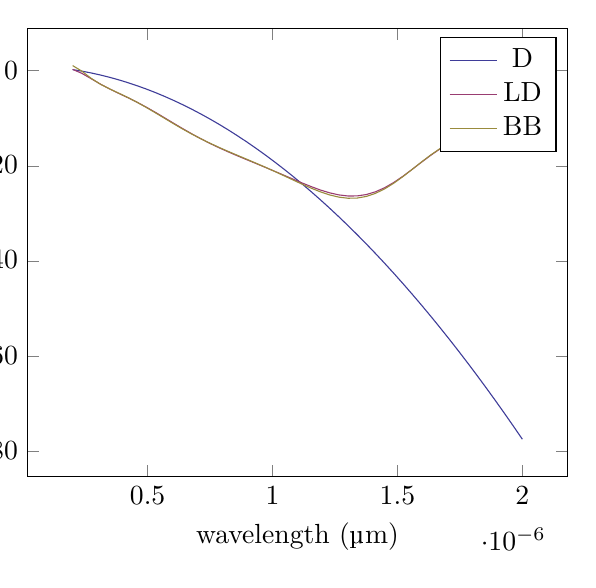
\begin{tikzpicture}[baseline,trim axis left]
			\begin{axis}[xlabel=wavelength (\si{\micro\meter}),ylabel=permittivity $\epsilon'$]
				\addplot[color=colora] coordinates {
						(2e-07, 0.20322363607787974)
						(2.3673469387755102e-07, -0.11627517562959966)
						(2.7346938775510205e-07, -0.48946741216304424)
						(3.1020408163265303e-07, -0.9163279342280204)
						(3.4693877551020406e-07, -1.3968279944952111)
						(3.836734693877551e-07, -1.9309352424380366)
						(4.2040816326530607e-07, -2.518613729774391)
						(4.571428571428571e-07, -3.1598239165107787)
						(4.938775510204081e-07, -3.854522677586954)
						(5.306122448979591e-07, -4.602663310118995)
						(5.673469387755102e-07, -5.40419554123853)
						(6.040816326530612e-07, -6.259065536525652)
						(6.408163265306121e-07, -7.167215909032926)
						(6.775510204081632e-07, -8.128585728897628)
						(7.142857142857142e-07, -9.143110533539227)
						(7.510204081632653e-07, -10.210722338438954)
						(7.877551020408163e-07, -11.331349648498069)
						(8.244897959183672e-07, -12.50491746997132)
						(8.612244897959183e-07, -13.731347322971876)
						(8.979591836734693e-07, -15.010557254543816)
						(9.346938775510204e-07, -16.342461852298243)
						(9.714285714285713e-07, -17.726972258608626)
						(1.0081632653061223e-06, -19.163996185361206)
						(1.0448979591836734e-06, -20.653437929255638)
						(1.0816326530612245e-06, -22.195198387651484)
						(1.1183673469387754e-06, -23.789175074955367)
						(1.1551020408163265e-06, -25.435262139544065)
						(1.1918367346938776e-06, -27.133350381218044)
						(1.2285714285714284e-06, -28.883327269180366)
						(1.2653061224489795e-06, -30.685076960535394)
						(1.3020408163265306e-06, -32.53848031930155)
						(1.3387755102040815e-06, -34.44341493593253)
						(1.3755102040816325e-06, -36.399755147341004)
						(1.4122448979591836e-06, -38.40737205741857)
						(1.4489795918367345e-06, -40.466133558046124)
						(1.4857142857142856e-06, -42.57590435058799)
						(1.5224489795918367e-06, -44.7365459678635)
						(1.5591836734693875e-06, -46.94791679658943)
						(1.5959183673469386e-06, -49.209872100286645)
						(1.6326530612244897e-06, -51.52226404264401)
						(1.6693877551020408e-06, -53.884941711332615)
						(1.7061224489795917e-06, -56.297751142263586)
						(1.7428571428571427e-06, -58.76053534428173)
						(1.7795918367346938e-06, -61.27313432428832)
						(1.8163265306122447e-06, -63.83538511278523)
						(1.8530612244897958e-06, -66.44712178983335)
						(1.8897959183673469e-06, -69.10817551141706)
						(1.9265306122448977e-06, -71.81837453620786)
						(1.963265306122449e-06, -74.57754425271895)
						(2e-06, -77.38550720684296)
					};
				\addlegendentry{D}
				\addplot[color=colorb] coordinates {
						(2e-07, 0.25231555087179547)
						(2.3673469387755102e-07, -0.575559020166577)
						(2.7346938775510205e-07, -1.6856206384322883)
						(3.1020408163265303e-07, -2.803697911637883)
						(3.4693877551020406e-07, -3.8266126296313816)
						(3.836734693877551e-07, -4.760897018999788)
						(4.2040816326530607e-07, -5.670759349056189)
						(4.571428571428571e-07, -6.621652898564422)
						(4.938775510204081e-07, -7.646949587694921)
						(5.306122448979591e-07, -8.744847848669961)
						(5.673469387755102e-07, -9.890905125412504)
						(6.040816326530612e-07, -11.052020645782637)
						(6.408163265306121e-07, -12.196291430759478)
						(6.775510204081632e-07, -13.298529435087051)
						(7.142857142857142e-07, -14.342689665025201)
						(7.510204081632653e-07, -15.322301457798549)
						(7.877551020408163e-07, -16.239591568820757)
						(8.244897959183672e-07, -17.103732324452302)
						(8.612244897959183e-07, -17.92853873002955)
						(8.979591836734693e-07, -18.729894716242526)
						(9.346938775510204e-07, -19.52315284945898)
						(9.714285714285713e-07, -20.320702660493506)
						(1.0081632653061223e-06, -21.129844835496602)
						(1.0448979591836734e-06, -21.951057590900447)
						(1.0816326530612245e-06, -22.77671313314228)
						(1.1183673469387754e-06, -23.590304871998622)
						(1.1551020408163265e-06, -24.366278988827602)
						(1.1918367346938776e-06, -25.07061512361259)
						(1.2285714285714284e-06, -25.662346644918607)
						(1.2653061224489795e-06, -26.09621591379901)
						(1.3020408163265306e-06, -26.326581669451887)
						(1.3387755102040815e-06, -26.31249794973732)
						(1.3755102040816325e-06, -26.023561936650985)
						(1.4122448979591836e-06, -25.44573850461694)
						(1.4489795918367345e-06, -24.586045334508746)
						(1.4857142857142856e-06, -23.474904922398423)
						(1.5224489795918367e-06, -22.16528059326988)
						(1.5591836734693875e-06, -20.728406576439504)
						(1.5959183673469386e-06, -19.246790629378406)
						(1.6326530612244897e-06, -17.805876994559092)
						(1.6693877551020408e-06, -16.486021211595826)
						(1.7061224489795917e-06, -15.356169628933038)
						(1.7428571428571427e-06, -14.470016364543326)
						(1.7795918367346938e-06, -13.86471222206908)
						(1.8163265306122447e-06, -13.561668219190409)
						(1.8530612244897958e-06, -13.568739780537314)
						(1.8897959183673469e-06, -13.883071570860366)
						(1.9265306122448977e-06, -14.494031564919382)
						(1.963265306122449e-06, -15.385864950612799)
						(2e-06, -16.539883792865695)
					};
				\addlegendentry{LD}
				\addplot[color=colorc] coordinates {
						(2e-07, 1.0504637003030624)
						(2.3673469387755102e-07, -0.11572802131651061)
						(2.7346938775510205e-07, -1.602682563793277)
						(3.1020408163265303e-07, -2.8350010015944944)
						(3.4693877551020406e-07, -3.8230067197317537)
						(3.836734693877551e-07, -4.717246821334378)
						(4.2040816326530607e-07, -5.636170653888561)
						(4.571428571428571e-07, -6.632604561214903)
						(4.938775510204081e-07, -7.7102347886976945)
						(5.306122448979591e-07, -8.84618877783769)
						(5.673469387755102e-07, -10.007477461824298)
						(6.040816326530612e-07, -11.161036854983045)
						(6.408163265306121e-07, -12.279422871974507)
						(6.775510204081632e-07, -13.343759250574305)
						(7.142857142857142e-07, -14.344820936601714)
						(7.510204081632653e-07, -15.282718538547668)
						(7.877551020408163e-07, -16.165508142356224)
						(8.244897959183672e-07, -17.007045137377226)
						(8.612244897959183e-07, -17.8244152816535)
						(8.979591836734693e-07, -18.63525266974235)
						(9.346938775510204e-07, -19.455185727600448)
						(9.714285714285713e-07, -20.29556213867539)
						(1.0081632653061223e-06, -21.161522602355504)
						(1.0448979591836734e-06, -22.05044555146455)
						(1.0816326530612245e-06, -22.950782526471528)
						(1.1183673469387754e-06, -23.84134755361321)
						(1.1551020408163265e-06, -24.691203780732366)
						(1.1918367346938776e-06, -25.460384312754776)
						(1.2285714285714284e-06, -26.10175203159548)
						(1.2653061224489795e-06, -26.564287055193436)
						(1.3020408163265306e-06, -26.797925741945612)
						(1.3387755102040815e-06, -26.75972499379113)
						(1.3755102040816325e-06, -26.42063225225901)
						(1.4122448979591836e-06, -25.771660931819127)
						(1.4489795918367345e-06, -24.828041106627545)
						(1.4857142857142856e-06, -23.630138313424883)
						(1.5224489795918367e-06, -22.240629502995787)
						(1.5591836734693875e-06, -20.738372207484858)
						(1.5959183673469386e-06, -19.210233052149597)
						(1.6326530612244897e-06, -17.74254102631741)
						(1.6693877551020408e-06, -16.413700445744936)
						(1.7061224489795917e-06, -15.288972326899973)
						(1.7428571428571427e-06, -14.417767545922914)
						(1.7795918367346938e-06, -13.833226868737341)
						(1.8163265306122447e-06, -13.553519596757006)
						(1.8530612244897958e-06, -13.584185305183397)
						(1.8897959183673469e-06, -13.920909049037)
						(1.9265306122448977e-06, -14.552274881994165)
						(1.963265306122449e-06, -15.46221509520403)
						(2e-06, -16.632020493319295)
					};
				\addlegendentry{BB}
			\end{axis}
		\end{tikzpicture}%
		\\
		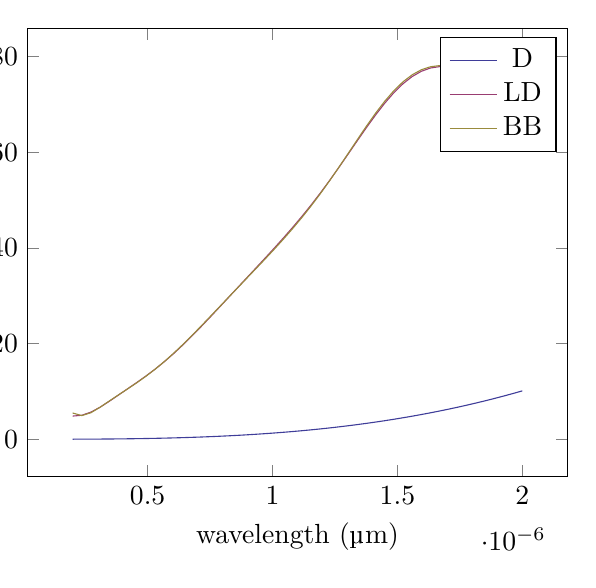
\begin{tikzpicture}[baseline,trim axis left]
			\begin{axis}[xlabel=wavelength (\si{\micro\meter}),ylabel=permittivity $\epsilon''$]
				\addplot[color=colora] coordinates {
						(2e-07, 0.010282295634328328)
						(2.3673469387755102e-07, 0.017051273651015157)
						(2.7346938775510205e-07, 0.026282300256503112)
						(3.1020408163265303e-07, 0.038356677993251154)
						(3.4693877551020406e-07, 0.05365539028535268)
						(3.836734693877551e-07, 0.07255905879799082)
						(4.2040816326530607e-07, 0.09544790088208063)
						(4.571428571428571e-07, 0.1227016871140709)
						(4.938775510204081e-07, 0.15469969894083985)
						(5.306122448979591e-07, 0.19182068643957828)
						(5.673469387755102e-07, 0.23444282620250456)
						(6.040816326530612e-07, 0.28294367935620796)
						(6.408163265306121e-07, 0.33770014972536283)
						(6.775510204081632e-07, 0.39908844215049616)
						(7.142857142857142e-07, 0.46748402096942987)
						(7.510204081632653e-07, 0.5432615686719579)
						(7.877551020408163e-07, 0.626794944737239)
						(8.244897959183672e-07, 0.7184571446633264)
						(8.612244897959183e-07, 0.8186202591981668)
						(8.979591836734693e-07, 0.9276554337813232)
						(9.346938775510204e-07, 1.0459328282056073)
						(9.714285714285713e-07, 1.1738215765076891)
						(1.0081632653061223e-06, 1.3116897470967004)
						(1.0448979591836734e-06, 1.4599043031297065)
						(1.0816326530612245e-06, 1.6188310631428795)
						(1.1183673469387754e-06, 1.7888346619470452)
						(1.1551020408163265e-06, 1.9702785117962387)
						(1.1918367346938776e-06, 2.1635247638377093)
						(1.2285714285714284e-06, 2.3689342698518128)
						(1.2653061224489795e-06, 2.5868665442900154)
						(1.3020408163265306e-06, 2.8176797266191755)
						(1.3387755102040815e-06, 3.061730543980143)
						(1.3755102040816325e-06, 3.3193742741685757)
						(1.4122448979591836e-06, 3.5909647089457524)
						(1.4489795918367345e-06, 3.876854117687057)
						(1.4857142857142856e-06, 4.177393211375655)
						(1.5224489795918367e-06, 4.4929311069487445)
						(1.5591836734693875e-06, 4.823815292003653)
						(1.5959183673469386e-06, 5.170391589870909)
						(1.6326530612244897e-06, 5.5330041250612485)
						(1.6693877551020408e-06, 5.911995289093416)
						(1.7061224489795917e-06, 6.307705706709462)
						(1.7428571428571427e-06, 6.720474202484044)
						(1.7795918367346938e-06, 7.150637767834207)
						(1.8163265306122447e-06, 7.5985315284357915)
						(1.8530612244897958e-06, 8.064488712052716)
						(1.8897959183673469e-06, 8.548840616784894)
						(1.9265306122448977e-06, 9.05191657974073)
						(1.963265306122449e-06, 9.574043946139808)
						(2e-06, 10.11554803885112)
					};
				\addlegendentry{D}
				\addplot[color=colorb] coordinates {
						(2e-07, 4.842797676957769)
						(2.3673469387755102e-07, 5.016762313321246)
						(2.7346938775510205e-07, 5.68256857090757)
						(3.1020408163265303e-07, 6.711979865081146)
						(3.4693877551020406e-07, 7.945793553037269)
						(3.836734693877551e-07, 9.25227171070903)
						(4.2040816326530607e-07, 10.564606804340109)
						(4.571428571428571e-07, 11.882172358378616)
						(4.938775510204081e-07, 13.241168914909778)
						(5.306122448979591e-07, 14.682767345030568)
						(5.673469387755102e-07, 16.235118510605385)
						(6.040816326530612e-07, 17.9085722463076)
						(6.408163265306121e-07, 19.697901267415105)
						(6.775510204081632e-07, 21.586904397315916)
						(7.142857142857142e-07, 23.553235356632428)
						(7.510204081632653e-07, 25.572705660194323)
						(7.877551020408163e-07, 27.62283714866403)
						(8.244897959183672e-07, 29.68558102301449)
						(8.612244897959183e-07, 31.74916054351672)
						(8.979591836734693e-07, 33.809035238024165)
						(9.346938775510204e-07, 35.868036529620426)
						(9.714285714285713e-07, 37.935770205791115)
						(1.0081632653061223e-06, 40.02740342833329)
						(1.0448979591836734e-06, 42.161948456634924)
						(1.0816326530612245e-06, 44.360129898336154)
						(1.1183673469387754e-06, 46.64189362650267)
						(1.1551020408163265e-06, 49.02360381875178)
						(1.1918367346938776e-06, 51.514999708750764)
						(1.2285714285714284e-06, 54.11606028282349)
						(1.2653061224489795e-06, 56.81405598050357)
						(1.3020408163265306e-06, 59.58123227092353)
						(1.3387755102040815e-06, 62.373719815919436)
						(1.3755102040816325e-06, 65.13231592918311)
						(1.4122448979591836e-06, 67.78563588320819)
						(1.4489795918367345e-06, 70.25573096208808)
						(1.4857142857142856e-06, 72.46565498933892)
						(1.5224489795918367e-06, 74.34781131015409)
						(1.5591836734693875e-06, 75.85149883634992)
						(1.5959183673469386e-06, 76.94812820215466)
						(1.6326530612244897e-06, 77.6331357523255)
						(1.6693877551020408e-06, 77.92448110410551)
						(1.7061224489795917e-06, 77.85843278961231)
						(1.7428571428571427e-06, 77.48383613647874)
						(1.7795918367346938e-06, 76.85611662026254)
						(1.8163265306122447e-06, 76.0319929307616)
						(1.8530612244897958e-06, 75.06544598445969)
						(1.8897959183673469e-06, 74.00508671150348)
						(1.9265306122448977e-06, 72.89278368864885)
						(1.963265306122449e-06, 71.76327028126319)
						(2e-06, 70.64442057895376)
					};
				\addlegendentry{LD}
				\addplot[color=colorc] coordinates {
						(2e-07, 5.487586152733378)
						(2.3673469387755102e-07, 4.943290733731911)
						(2.7346938775510205e-07, 5.552879873741859)
						(3.1020408163265303e-07, 6.709285142615963)
						(3.4693877551020406e-07, 8.004405136835327)
						(3.836734693877551e-07, 9.284298761856535)
						(4.2040816326530607e-07, 10.543809390982444)
						(4.571428571428571e-07, 11.830248269055213)
						(4.938775510204081e-07, 13.192785928242087)
						(5.306122448979591e-07, 14.664395567592711)
						(5.673469387755102e-07, 16.259059400805672)
						(6.040816326530612e-07, 17.974516399602148)
						(6.408163265306121e-07, 19.796551905891018)
						(6.775510204081632e-07, 21.703483515920034)
						(7.142857142857142e-07, 23.670409426121562)
						(7.510204081632653e-07, 25.67299281883518)
						(7.877551020408163e-07, 27.690577764205813)
						(8.244897959183672e-07, 29.70846787521698)
						(8.612244897959183e-07, 31.71928580236796)
						(8.979591836734693e-07, 33.72343892941241)
						(9.346938775510204e-07, 35.728801977788564)
						(9.714285714285713e-07, 37.74976503347855)
						(1.0081632653061223e-06, 39.80578353708523)
						(1.0448979591836734e-06, 41.91952013353689)
						(1.0816326530612245e-06, 44.114610442271776)
						(1.1183673469387754e-06, 46.41304159797824)
						(1.1551020408163265e-06, 48.83212964840445)
						(1.1918367346938776e-06, 51.38114369198234)
						(1.2285714285714284e-06, 54.05776738230274)
						(1.2653061224489795e-06, 56.84480656354894)
						(1.3020408163265306e-06, 59.70779731452721)
						(1.3387755102040815e-06, 62.594337776255024)
						(1.3755102040816325e-06, 65.43591866714534)
						(1.4122448979591836e-06, 68.1526509000506)
						(1.4489795918367345e-06, 70.66060186459768)
						(1.4857142857142856e-06, 72.88065667112629)
						(1.5224489795918367e-06, 74.74724354310236)
						(1.5591836734693875e-06, 76.21518368762695)
						(1.5959183673469386e-06, 77.2634068687876)
						(1.6326530612244897e-06, 77.89511553406447)
						(1.6693877551020408e-06, 78.13484250349717)
						(1.7061224489795917e-06, 78.02343488487479)
						(1.7428571428571427e-06, 77.61218566362417)
						(1.7795918367346938e-06, 76.9571776773715)
						(1.8163265306122447e-06, 76.11455506919033)
						(1.8530612244897958e-06, 75.13705356998602)
						(1.8897959183673469e-06, 74.07180995746026)
						(1.9265306122448977e-06, 72.95927499369772)
						(1.963265306122449e-06, 71.83296695393076)
						(2e-06, 70.71979471932364)
					};
				\addlegendentry{BB}
			\end{axis}
		\end{tikzpicture}%
		\\
		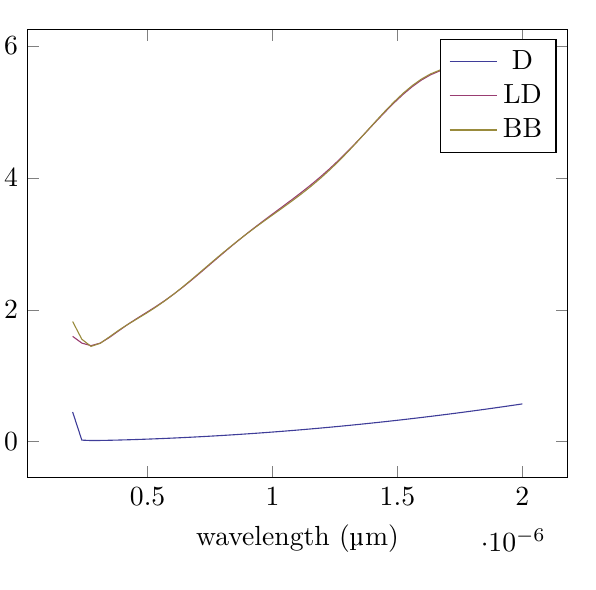
\begin{tikzpicture}[baseline,trim axis left]
			\begin{axis}[xlabel=wavelength (\si{\micro\meter}),ylabel=refractive index $n'$]
				\addplot[color=colora] coordinates {
						(2e-07, 0.45094746213961884)
						(2.3673469387755102e-07, 0.024935908286396326)
						(2.7346938775510205e-07, 0.018776521253925264)
						(3.1020408163265303e-07, 0.02003043909408883)
						(3.4693877551020406e-07, 0.0226950864396265)
						(3.836734693877551e-07, 0.026103646266798116)
						(4.2040816326530607e-07, 0.030066140248912892)
						(4.571428571428571e-07, 0.03450700638553323)
						(4.938775510204081e-07, 0.03939007236413651)
						(5.306122448979591e-07, 0.04469578947703119)
						(5.673469387755102e-07, 0.05041262724118856)
						(6.040816326530612e-07, 0.056533308157751705)
						(6.408163265306121e-07, 0.06305297679096514)
						(6.775510204081632e-07, 0.06996823506724477)
						(7.142857142857142e-07, 0.0772766007944913)
						(7.510204081632653e-07, 0.0849761877532624)
						(7.877551020408163e-07, 0.09306550850470252)
						(8.244897959183672e-07, 0.10154334842125644)
						(8.612244897959183e-07, 0.11040868272282886)
						(8.979591836734693e-07, 0.11966062037667895)
						(9.346938775510204e-07, 0.12929836527979136)
						(9.714285714285713e-07, 0.13932118885028524)
						(1.0081632653061223e-06, 0.14972841032465903)
						(1.0448979591836734e-06, 0.160519382366376)
						(1.0816326530612245e-06, 0.17169348040314722)
						(1.1183673469387754e-06, 0.18325009462506753)
						(1.1551020408163265e-06, 0.19518862391035868)
						(1.1918367346938776e-06, 0.2075084711668404)
						(1.2285714285714284e-06, 0.22020903972608502)
						(1.2653061224489795e-06, 0.23328973052956503)
						(1.3020408163265306e-06, 0.2467499399170699)
						(1.3387755102040815e-06, 0.260589057877576)
						(1.3755102040816325e-06, 0.2748064666586697)
						(1.4122448979591836e-06, 0.28940153965625487)
						(1.4489795918367345e-06, 0.30437364052529614)
						(1.4857142857142856e-06, 0.3197221224660584)
						(1.5224489795918367e-06, 0.3354463276509178)
						(1.5591836734693875e-06, 0.3515455867643492)
						(1.5959183673469386e-06, 0.36801921863480275)
						(1.6326530612244897e-06, 0.3848665299415491)
						(1.6693877551020408e-06, 0.40208681498312016)
						(1.7061224489795917e-06, 0.41967935549672253)
						(1.7428571428571427e-06, 0.4376434205198815)
						(1.7795918367346938e-06, 0.4559782662874944)
						(1.8163265306122447e-06, 0.47468313615862195)
						(1.8530612244897958e-06, 0.4937572605683653)
						(1.8897959183673469e-06, 0.5131998570010436)
						(1.9265306122448977e-06, 0.5330101299816713)
						(1.963265306122449e-06, 0.55318727108296)
						(2e-06, 0.5737304589458854)
					};
				\addlegendentry{D}
				\addplot[color=colorb] coordinates {
						(2e-07, 1.597135207835735)
						(2.3673469387755102e-07, 1.495679025267232)
						(2.7346938775510205e-07, 1.4563105460899657)
						(3.1020408163265303e-07, 1.4950458292474733)
						(3.4693877551020406e-07, 1.579969143527494)
						(3.836734693877551e-07, 1.6799438087477938)
						(4.2040816326530607e-07, 1.7775809344758216)
						(4.571428571428571e-07, 1.868288680797464)
						(4.938775510204081e-07, 1.954957029756189)
						(5.306122448979591e-07, 2.0426451904533183)
						(5.673469387755102e-07, 2.1353989109147187)
						(6.040816326530612e-07, 2.2352087559974385)
						(6.408163265306121e-07, 2.3421914782910904)
						(6.775510204081632e-07, 2.4551848388523108)
						(7.142857142857142e-07, 2.5723421355535767)
						(7.510204081632653e-07, 2.691595939878992)
						(7.877551020408163e-07, 2.810985381458551)
						(8.244897959183672e-07, 2.928874760655689)
						(8.612244897959183e-07, 3.044090263165657)
						(8.979591836734693e-07, 3.1559933517483523)
						(9.346938775510204e-07, 3.2645027959859383)
						(9.714285714285713e-07, 3.3700734320205914)
						(1.0081632653061223e-06, 3.4736377054222585)
						(1.0448979591836734e-06, 3.5765149175586335)
						(1.0816326530612245e-06, 3.6802924255907072)
						(1.1183673469387754e-06, 3.7866828050860413)
						(1.1551020408163265e-06, 3.8973613659903283)
						(1.1918367346938776e-06, 4.013789698272117)
						(1.2285714285714284e-06, 4.137033381885216)
						(1.2653061224489795e-06, 4.267585743925975)
						(1.3020408163265306e-06, 4.405214291318991)
						(1.3387755102040815e-06, 4.548851137285941)
						(1.3755102040816325e-06, 4.6965513302213155)
						(1.4122448979591836e-06, 4.845540712993846)
						(1.4489795918367345e-06, 4.992365371593061)
						(1.4857142857142856e-06, 5.1331375702263875)
						(1.5224489795918367e-06, 5.2638516402973865)
						(1.5591836734693875e-06, 5.380724398777348)
						(1.5959183673469386e-06, 5.480505989705262)
						(1.6326530612244897e-06, 5.560713043670437)
						(1.6693877551020408e-06, 5.6197551320378)
						(1.7061224489795917e-06, 5.656950549174113)
						(1.7428571428571427e-06, 5.672449646650553)
						(1.7795918367346938e-06, 5.667097019325239)
						(1.8163265306122447e-06, 5.642266302648792)
						(1.8530612244897958e-06, 5.599695701458524)
						(1.8897959183673469e-06, 5.541342847015116)
						(1.9265306122448977e-06, 5.469267921204983)
						(1.963265306122449e-06, 5.385546427894745)
						(2e-06, 5.292208247659441)
					};
				\addlegendentry{LD}
				\addplot[color=colorc] coordinates {
						(2e-07, 1.8217694743404074)
						(2.3673469387755102e-07, 1.553852822618352)
						(2.7346938775510205e-07, 1.4451394438611898)
						(3.1020408163265303e-07, 1.491419020243556)
						(3.4693877551020406e-07, 1.5886314200834342)
						(3.836734693877551e-07, 1.6877079090542917)
						(4.2040816326530607e-07, 1.7775701835042848)
						(4.571428571428571e-07, 1.8614608250259643)
						(4.938775510204081e-07, 1.94555703371944)
						(5.306122448979591e-07, 2.0346746422372677)
						(5.673469387755102e-07, 2.13126475860591)
						(6.040816326530612e-07, 2.2357046896603836)
						(6.408163265306121e-07, 2.3469379391910756)
						(6.775510204081632e-07, 2.4630900296633733)
						(7.142857142857142e-07, 2.581957319106738)
						(7.510204081632653e-07, 2.701366820248984)
						(7.877551020408163e-07, 2.8194291725374483)
						(8.244897959183672e-07, 2.934705786582067)
						(8.612244897959183e-07, 3.046306080703066)
						(8.979591836734693e-07, 3.1539272916776797)
						(9.346938775510204e-07, 3.257847369495045)
						(9.714285714285713e-07, 3.3588797420814167)
						(1.0081632653061223e-06, 3.458296643721037)
						(1.0448979591836734e-06, 3.5577253498198695)
						(1.0816326530612245e-06, 3.6590195650383737)
						(1.1183673469387754e-06, 3.7641070098631593)
						(1.1551020408163265e-06, 3.8748145872688005)
						(1.1918367346938776e-06, 3.9926750011867322)
						(1.2285714285714284e-06, 4.118723790032171)
						(1.2653061224489795e-06, 4.253303302152364)
						(1.3020408163265306e-06, 4.39589879650376)
						(1.3387755102040815e-06, 4.5450384462016125)
						(1.3755102040816325e-06, 4.6982890444022845)
						(1.4122448979591836e-06, 4.8523687776815)
						(1.4489795918367345e-06, 5.00337726528504)
						(1.4857142857142856e-06, 5.14711639331484)
						(1.5224489795918367e-06, 5.279452676528295)
						(1.5591836734693875e-06, 5.396661916471713)
						(1.5959183673469386e-06, 5.495703479711868)
						(1.6326530612244897e-06, 5.5743912699159734)
						(1.6693877551020408e-06, 5.631453403456235)
						(1.7061224489795917e-06, 5.6664943775884264)
						(1.7428571428571427e-06, 5.67988693061195)
						(1.7795918367346938e-06, 5.672624786152883)
						(1.8163265306122447e-06, 5.646164113783168)
						(1.8530612244897958e-06, 5.6022741567360095)
						(1.8897959183673469e-06, 5.542909140310406)
						(1.9265306122448977e-06, 5.470106320733739)
						(1.963265306122449e-06, 5.385909793594694)
						(2e-06, 5.292316559410185)
					};
				\addlegendentry{BB}
			\end{axis}
		\end{tikzpicture}%
		\\
		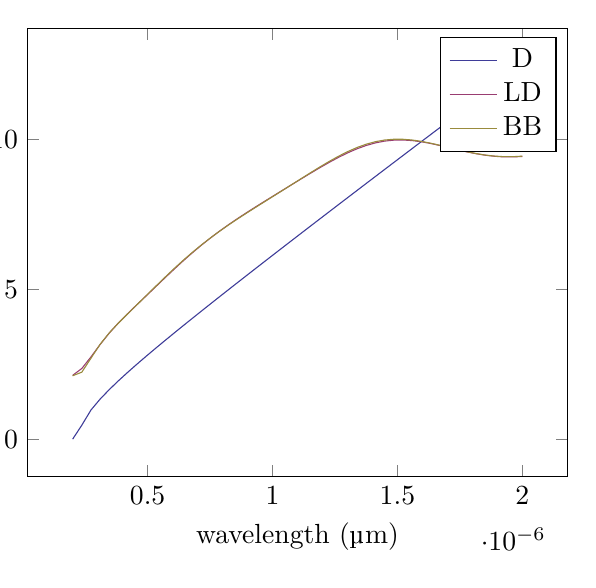
\begin{tikzpicture}[baseline,trim axis left]
			\begin{axis}[xlabel=wavelength (\si{\micro\meter}),ylabel=refractive index $n''$]
				\addplot[color=colora] coordinates {
						(2e-07, 0.016123122047746366)
						(2.3673469387755102e-07, 0.48352244033067837)
						(2.7346938775510205e-07, 0.9897676191040434)
						(3.1020408163265303e-07, 1.3540525489938138)
						(3.4693877551020406e-07, 1.6717314745159961)
						(3.836734693877551e-07, 1.965510947711286)
						(4.2040816326530607e-07, 2.2447795894313805)
						(4.571428571428571e-07, 2.514364591701239)
						(4.938775510204081e-07, 2.7770755320616707)
						(5.306122448979591e-07, 3.0346864825599265)
						(5.673469387755102e-07, 3.288384702015228)
						(6.040816326530612e-07, 3.539000297105642)
						(6.408163265306121e-07, 3.7871338996436683)
						(6.775510204081632e-07, 4.033232272710326)
						(7.142857142857142e-07, 4.277635376366148)
						(7.510204081632653e-07, 4.5206068820290115)
						(7.877551020408163e-07, 4.762354635549794)
						(8.244897959183672e-07, 5.003044777249134)
						(8.612244897959183e-07, 5.242811726581924)
						(8.979591836734693e-07, 5.4817653942161275)
						(9.346938775510204e-07, 5.719996489432885)
						(9.714285714285713e-07, 5.957580490815258)
						(1.0081632653061223e-06, 6.1945806609034575)
						(1.0448979591836734e-06, 6.43105036543346)
						(1.0816326530612245e-06, 6.667034878994474)
						(1.1183673469387754e-06, 6.90257280615503)
						(1.1551020408163265e-06, 7.137697211068579)
						(1.1918367346938776e-06, 7.3724365235414595)
						(1.2285714285714284e-06, 7.606815271893679)
						(1.2653061224489795e-06, 7.840854680314634)
						(1.3020408163265306e-06, 8.074573159263668)
						(1.3387755102040815e-06, 8.307986710752257)
						(1.3755102040816325e-06, 8.54110926536576)
						(1.4122448979591836e-06, 8.773952964151789)
						(1.4489795918367345e-06, 9.00652839567974)
						(1.4857142857142856e-06, 9.238844796421485)
						(1.5224489795918367e-06, 9.470910220944763)
						(1.5591836734693875e-06, 9.702731687124293)
						(1.5959183673469386e-06, 9.934315300570162)
						(1.6326530612244897e-06, 10.165666361681684)
						(1.6693877551020408e-06, 10.396789458108294)
						(1.7061224489795917e-06, 10.627688544899472)
						(1.7428571428571427e-06, 10.85836701422512)
						(1.7795918367346938e-06, 11.08882775622517)
						(1.8163265306122447e-06, 11.319073212285414)
						(1.8530612244897958e-06, 11.549105421823572)
						(1.8897959183673469e-06, 11.778926063495174)
						(1.9265306122448977e-06, 12.008536491585554)
						(1.963265306122449e-06, 12.237937768235884)
						(2e-06, 12.46713069205302)
					};
				\addlegendentry{D}
				\addplot[color=colorb] coordinates {
						(2e-07, 2.144073376186879)
						(2.3673469387755102e-07, 2.3717566345605166)
						(2.7346938775510205e-07, 2.759152422424373)
						(3.1020408163265303e-07, 3.1745424688254364)
						(3.4693877551020406e-07, 3.556097615119806)
						(3.836734693877551e-07, 3.8943826775369246)
						(4.2040816326530607e-07, 4.202511945888584)
						(4.571428571428571e-07, 4.497144759369071)
						(4.938775510204081e-07, 4.789322828101707)
						(5.306122448979591e-07, 5.08276444914616)
						(5.673469387755102e-07, 5.376027089617066)
						(6.040816326530612e-07, 5.6653647417743995)
						(6.408163265306121e-07, 5.946789445026431)
						(6.775510204081632e-07, 6.217147581973151)
						(7.142857142857142e-07, 6.474509051251614)
						(7.510204081632653e-07, 6.718182814031131)
						(7.877551020408163e-07, 6.948558179017347)
						(8.244897959183672e-07, 7.1668737519309245)
						(8.612244897959183e-07, 7.374960916551289)
						(8.979591836734693e-07, 7.574983663681702)
						(9.346938775510204e-07, 7.769186746945782)
						(9.714285714285713e-07, 7.9596604949840115)
						(1.0081632653061223e-06, 8.148129079000629)
						(1.0448979591836734e-06, 8.335768296494319)
						(1.0816326530612245e-06, 8.52305877851404)
						(1.1183673469387754e-06, 8.709680997411205)
						(1.1551020408163265e-06, 8.894459467099908)
						(1.1918367346938776e-06, 9.075364771243958)
						(1.2285714285714284e-06, 9.249582893055365)
						(1.2653061224489795e-06, 9.413660711493614)
						(1.3020408163265306e-06, 9.563733018219713)
						(1.3387755102040815e-06, 9.695828445153609)
						(1.3755102040816325e-06, 9.806238456620825)
						(1.4122448979591836e-06, 9.891916225473997)
						(1.4489795918367345e-06, 9.950854972110715)
						(1.4857142857142856e-06, 9.982385109508456)
						(1.5224489795918367e-06, 9.987333446354073)
						(1.5591836734693875e-06, 9.96800899197401)
						(1.5959183673469386e-06, 9.928014558064836)
						(1.6326530612244897e-06, 9.87192043612646)
						(1.6693877551020408e-06, 9.804862972592836)
						(1.7061224489795917e-06, 9.732138423258718)
						(1.7428571428571427e-06, 9.658851003957906)
						(1.7795918367346938e-06, 9.589650759909256)
						(1.8163265306122447e-06, 9.528571482567203)
						(1.8530612244897958e-06, 9.478958986035375)
						(1.8897959183673469e-06, 9.443468866791054)
						(1.9265306122448977e-06, 9.424109842191067)
						(1.963265306122449e-06, 9.422311317041341)
						(2e-06, 9.438999092007617)
					};
				\addlegendentry{LD}
				\addplot[color=colorc] coordinates {
						(2e-07, 2.129967284882781)
						(2.3673469387755102e-07, 2.2495273350975444)
						(2.7346938775510205e-07, 2.717024319359952)
						(3.1020408163265303e-07, 3.180984657472822)
						(3.4693877551020406e-07, 3.5627956743568845)
						(3.836734693877551e-07, 3.889885552974223)
						(4.2040816326530607e-07, 4.194264276645433)
						(4.571428571428571e-07, 4.493916101647036)
						(4.938775510204081e-07, 4.794877883774077)
						(5.306122448979591e-07, 5.096290744767423)
						(5.673469387755102e-07, 5.394398378521892)
						(6.040816326530612e-07, 5.684964786936236)
						(6.408163265306121e-07, 5.96448498403491)
						(6.775510204081632e-07, 6.230661561150858)
						(7.142857142857142e-07, 6.482487876470047)
						(7.510204081632653e-07, 6.720134111175129)
						(7.877551020408163e-07, 6.944737432230455)
						(8.244897959183672e-07, 7.158148250934106)
						(8.612244897959183e-07, 7.362662021168971)
						(8.979591836734693e-07, 7.560755257371006)
						(9.346938775510204e-07, 7.754837872003029)
						(9.714285714285713e-07, 7.947029037374951)
						(1.0081632653061223e-06, 8.13896041006807)
						(1.0448979591836734e-06, 8.331609114236633)
						(1.0816326530612245e-06, 8.525163541399676)
						(1.1183673469387754e-06, 8.718927587188023)
						(1.1551020408163265e-06, 8.911272845833356)
						(1.1918367346938776e-06, 9.099652518404893)
						(1.2285714285714284e-06, 9.280693690686324)
						(1.2653061224489795e-06, 9.450383699648777)
						(1.3020408163265306e-06, 9.604358590874126)
						(1.3387755102040815e-06, 9.738285215708348)
						(1.3755102040816325e-06, 9.848304645674762)
						(1.4122448979591836e-06, 9.931479616495961)
						(1.4489795918367345e-06, 9.986172957184223)
						(1.4857142857142856e-06, 10.012286999457741)
						(1.5224489795918367e-06, 10.011318601133176)
						(1.5591836734693875e-06, 9.986223715517392)
						(1.5959183673469386e-06, 9.94112566956748)
						(1.6326530612244897e-06, 9.88092901061766)
						(1.6693877551020408e-06, 9.810909018133207)
						(1.7061224489795917e-06, 9.736337181727142)
						(1.7428571428571427e-06, 9.662182268044766)
						(1.7795918367346938e-06, 9.592903505530886)
						(1.8163265306122447e-06, 9.532333271191256)
						(1.8530612244897958e-06, 9.48363443331886)
						(1.8897959183673469e-06, 9.449312227540547)
						(1.9265306122448977e-06, 9.431260577687944)
						(1.963265306122449e-06, 9.430825987149086)
						(2e-06, 9.448876658981908)
					};
				\addlegendentry{BB}
			\end{axis}
		\end{tikzpicture}%
		\\
	\end{tabular}
	\caption{Complex permittivity $\epsilon = \epsilon' + \mi \epsilon''$ and refractive index $n = n' + \mi n''$ for Pt based on the Drude (D), Lorentz-Drude (LD), and Brendel-Bormann (BB) models.}
\end{figure}
\clearpage


%\section{Three Layer Fresnel Data}
%\label{sec:threelayerfresnel}
%\pgfplotsset{
  /pgfplots/colormap={jet}{rgb255(0cm)=(0,0,128) rgb255(1cm)=(0,0,255)
      rgb255(3cm)=(0,255,255) rgb255(5cm)=(255,255,0) rgb255(7cm)=(255,0,0)
      rgb255(8cm)=(128,0,0)}
}

\subsection{Metal-BK7-Air}
\input{fresnel_plots/Ag_BK7_air_6328_0-100_0-90}
\input{fresnel_plots/Al_BK7_air_6328_0-100_0-90}
\input{fresnel_plots/Au_BK7_air_6328_0-100_0-90}
\newpage
\subsubsection{Be-BK7-$ \text{Vacuum} $}
\begin{figure}[h]
\pgfplotsset{
 small,
 width=0.8\textwidth,
 height=0.8\textwidth,
 enlargelimits=false,
 axis on top,
 legend pos = north east,
 empty legend,
 title = {$\lambda_0=\SI{632.8}{\nano\meter}$, $\epsilon_1=\text{BK7}$, $\epsilon_2=\text{Be}$, $\epsilon_3=\text{Vacuum}$},
 minor tick num=3,
 colorbar,
 colorbar style = { ylabel=$|\tilde{r}_{123}|$ },
 legend style = { cells = {anchor=west} }
}
\centering
\begin{tikzpicture}
\begin{axis}[
xlabel=angle (degrees),
ylabel=metal thickness (\si{\nano\meter}),
]
\addplot[mark=none] coordinates {(0,0)};
\addplot[mark=none] coordinates {(0,0)};
\addplot[mark=none] coordinates {(0,0)};
\addplot graphics 
[
xmin=0,
xmax=90,
ymin=0,
ymax=100
]{fresnel/Be_BK7_air_6328_0-100_0-90.png};
%\, $d=\SI{47.12761744}{\nano\meter}$,
%\legend{
%{\tiny $\lambda_0=\SI{632.8}{\nano\meter}$},
%{\tiny $\epsilon_1=\text{BK7}$},
%{\tiny $\epsilon_2=\text{Ag}$},
%{\tiny $\epsilon_3=\text{Vacuum}$},
%}

\end{axis}
\end{tikzpicture}
\caption{Reflection coefficent $|\tilde{r}_{123}|$ for the three layer fresnel
system (Be-BK7-$ \text{Vacuum} $)
as a function of incident angle and thickness of the metal layer
$\epsilon_2$.  Numeric values of the permittivity are found in
\Table{tbl:metalairtable}
}
\label{fig:3layerfresnelBe}
\end{figure}
\clearpage

\input{fresnel_plots/Cr_BK7_air_6328_0-100_0-90}
\input{fresnel_plots/Cu_BK7_air_6328_0-100_0-90}
\input{fresnel_plots/Ni_BK7_air_6328_0-100_0-90}
\input{fresnel_plots/Pd_BK7_air_6328_0-100_0-90}
\input{fresnel_plots/Pt_BK7_air_6328_0-100_0-90}
\input{fresnel_plots/Ti_BK7_air_6328_0-100_0-90}
\input{fresnel_plots/W_BK7_air_6328_0-100_0-90}
\subsection{Metal-LAH79-Air}
\input{fresnel_plots/Ag_LAH79_air_6328_0-100_0-90}
\input{fresnel_plots/Al_LAH79_air_6328_0-100_0-90}
\input{fresnel_plots/Au_LAH79_air_6328_0-100_0-90}
\input{fresnel_plots/Be_LAH79_air_6328_0-100_0-90}
\input{fresnel_plots/Cr_LAH79_air_6328_0-100_0-90}
\input{fresnel_plots/Cu_LAH79_air_6328_0-100_0-90}
\input{fresnel_plots/Ni_LAH79_air_6328_0-100_0-90}
\input{fresnel_plots/Pd_LAH79_air_6328_0-100_0-90}
\input{fresnel_plots/Pt_LAH79_air_6328_0-100_0-90}
\input{fresnel_plots/Ti_LAH79_air_6328_0-100_0-90}
\input{fresnel_plots/W_LAH79_air_6328_0-100_0-90}
\subsection{Metal-BK7-\ce{H2O}}
\input{fresnel_plots/Ag_BK7_h2o_6328_0-100_0-90}
\input{fresnel_plots/Al_BK7_h2o_6328_0-100_0-90}
\input{fresnel_plots/Au_BK7_h2o_6328_0-100_0-90}
\input{fresnel_plots/Be_BK7_h2o_6328_0-100_0-90}
\input{fresnel_plots/Cr_BK7_h2o_6328_0-100_0-90}
\input{fresnel_plots/Cu_BK7_h2o_6328_0-100_0-90}
\input{fresnel_plots/Ni_BK7_h2o_6328_0-100_0-90}
\input{fresnel_plots/Pd_BK7_h2o_6328_0-100_0-90}
\input{fresnel_plots/Pt_BK7_h2o_6328_0-100_0-90}
\input{fresnel_plots/Ti_BK7_h2o_6328_0-100_0-90}
\input{fresnel_plots/W_BK7_h2o_6328_0-100_0-90}
\subsection{Metal-LAH79-\ce{H2O}}
\input{fresnel_plots/Ag_LAH79_h2o_6328_0-100_0-90}
\input{fresnel_plots/Al_LAH79_h2o_6328_0-100_0-90}
\input{fresnel_plots/Au_LAH79_h2o_6328_0-100_0-90}
\input{fresnel_plots/Be_LAH79_h2o_6328_0-100_0-90}
\input{fresnel_plots/Cr_LAH79_h2o_6328_0-100_0-90}
\input{fresnel_plots/Cu_LAH79_h2o_6328_0-100_0-90}
\input{fresnel_plots/Ni_LAH79_h2o_6328_0-100_0-90}
\input{fresnel_plots/Pd_LAH79_h2o_6328_0-100_0-90}
\input{fresnel_plots/Pt_LAH79_h2o_6328_0-100_0-90}
\input{fresnel_plots/Ti_LAH79_h2o_6328_0-100_0-90}
\input{fresnel_plots/W_LAH79_h2o_6328_0-100_0-90}


\section{Abbreviations}
%\input{abbreviations}
\end{document}
